%!TEX root = ../main.tex
\section{System Verification}
\label{sec:system_verification}
\thomas{Add verification subsection, indent every verification to subsubsection}
\thomas{write introduction to this section}
\subsection{Verification of: Requirements \ref{enum:system_consists_double_pendulum} and \ref{enum:cart_actuated_by_motor}} % (fold)
\label{sub:verification_of_requirement_enum:system_consists_double_pendulum}
These requirements specify that the system should consist of a double pendulum mounted on a moveable cart and that the cart should be actuated by a motor.

\paragraph{Conclusion}~\\
The implemented system consists of the designed and implemented pendulum assembly mounted on the rail system inherited from an earlier project.
A picture of the full system setup is shown in figure \ref{fig:pic_full_system}.
Specific requirements for designing and implementing the pendulum assembly are described and verified in section \ref{sec:joint_development}.
\begin{figure}
	\centering
	\missingfigure{Picture of full system}
	\caption{Picture of full system.}
	\label{fig:pic_full_system}
\end{figure}
The cart can be actuated by the Maxon motor as they are connected by a belt. 
Even though the cart was never moved using the motor due to debugging troubles and time constraints, it was tested that the developed controller board is able to drive the motor.

\subsection{Verification of: Requirement \ref{enum:controlled_by_microzed}} % (fold)
\label{sub:verification_of_requirement_enum:controlled_by_microzed}
This requirement states that the pendulum system should be controlled by a MicroZed.

\paragraph{Conclusion}~\\
The controller board has been designed to fit the MicroZed and all relevant signals were wired to it as described in section \label{sec:controller_board}.
\\~\\
\thomas{insert correct reference}
In section \ref{subs:requirement_enum:motor_speed_direction} it was verified that the MicroZed can control motor speed and direction through implemented VHDL modules, the motor driver and the H-bridge on the controller board. 
\\~\\
In section \ref{ssub:requrement_enum:motor_current_} it was found that it is not possible to determine the motor current using a shunt resistor and the \texttt{INA286}. 
Thus it is not possible to measure the motor current using the ADC on the MicroZed.
\\~\\
In section \ref{ssub:requirement_enum:microzed_interface} it was verified that the MicroZed is interfaced correctly by measuring start-up and power-down sequences.



\subsection{Verification of: Requirement \ref{enum:position_cart_joint_angle_measure}} % (fold)
\label{sub:verification_of_requirement_enum:position_cart_joint_angle_measure}
According to this requirement the position of the cart and joint angles should be measured.

\paragraph{Test}~\\
In section \ref{ssub:verification_of_requirement_enum:correct_cart_position} it is tested and verified that the position of the cart is measured correctly. 
\\~\\
In section \ref{ssub:requirement_enum:correct_angles} it is verified by visual inspection that the joint angles are correctly measured on the joint board.
\\
To further verify that the measurement is correct a test should be conducted where the joint angle data are stored and plotted.  
In a single pendulum setup, the joint should manually be moved $\frac{\pi}{2}$ radians from the equilibrium position and released, while collecting joint angle data.

\paragraph{Conclusion}~\\
The test described above was conducted while transmitting data at 1kHz, with the two \texttt{nRFM}s pointing at each other.
An excerpt of the corresponding data is shown in figure \ref{fig:joint_angle_measured_full} with the joint angle measured in ticks.
A full rotation is equal to 7200 ticks.
As expected the waveform is a damped sinusoidal.
\begin{figure}[h]
	\centering
	% This file was created by matlab2tikz.
%
%The latest updates can be retrieved from
%  http://www.mathworks.com/matlabcentral/fileexchange/22022-matlab2tikz-matlab2tikz
%where you can also make suggestions and rate matlab2tikz.
%
\definecolor{mycolor1}{rgb}{0.00000,0.44700,0.74100}%
%
\begin{tikzpicture}

\begin{axis}[%
width=.9\textwidth,
height=2.5in,
at={(0.758in,0.481in)},
scale only axis,
xmin=60000,
xmax=100000,
xlabel style={font=\color{white!15!black}},
xlabel={Time [us]},
ymin=4000,
ymax=5200,
ylabel style={font=\color{white!15!black}},
ylabel={Angle [ticks]},
axis background/.style={fill=white},
title style={font=\bfseries},
title={Joint Angle Transmission},
axis x line*=bottom,
axis y line*=left
]
\addplot[only marks, mark=*, mark options={}, mark size=0.5000pt, draw=mycolor1] table[row sep=crcr]{%
x	y\\
58576	4739\\
58577	4742\\
58578	4746\\
58579	4750\\
58580	4753\\
58581	4757\\
58582	4761\\
58583	4764\\
58584	4768\\
58585	4771\\
58586	4775\\
58587	4779\\
58589	4786\\
58590	4789\\
58591	4793\\
58595	4807\\
58596	4810\\
58597	4814\\
58599	4821\\
58600	4824\\
58601	4828\\
58603	4835\\
58604	4838\\
58605	4841\\
58607	4848\\
58609	4855\\
58611	4861\\
58612	4864\\
58614	4871\\
58615	4874\\
58616	4877\\
58618	4883\\
58619	4886\\
58622	4896\\
58625	4905\\
58626	4908\\
58627	4911\\
58629	4917\\
58630	4920\\
58632	4926\\
58633	4929\\
58634	4932\\
58635	4934\\
58636	4937\\
58637	4940\\
58638	4943\\
58640	4948\\
58641	4951\\
58642	4954\\
58644	4959\\
58645	4962\\
58646	4964\\
58647	4967\\
58650	4975\\
58652	4980\\
58654	4985\\
58655	4987\\
58656	4989\\
58657	4992\\
58658	4994\\
58659	4996\\
58660	4999\\
58661	5001\\
58663	5006\\
58665	5010\\
58666	5012\\
58667	5015\\
58668	5017\\
58671	5023\\
58672	5025\\
58673	5027\\
58674	5029\\
58676	5033\\
58677	5035\\
58678	5037\\
58680	5041\\
58682	5044\\
58683	5046\\
58684	5048\\
58686	5052\\
58687	5053\\
58688	5055\\
58689	5057\\
58690	5058\\
58691	5060\\
58693	5063\\
58694	5064\\
58695	5066\\
58696	5067\\
58697	5069\\
58698	5070\\
58699	5071\\
58700	5073\\
58701	5074\\
58702	5075\\
58703	5077\\
58704	5078\\
58705	5079\\
58706	5080\\
58707	5082\\
58708	5083\\
58710	5085\\
58711	5086\\
58712	5087\\
58715	5090\\
58716	5091\\
58717	5092\\
58718	5093\\
58720	5095\\
58721	5095\\
58722	5096\\
58725	5099\\
58726	5099\\
58727	5100\\
58728	5101\\
58730	5102\\
58737	5105\\
58738	5106\\
58740	5106\\
58741	5107\\
58743	5107\\
58744	5108\\
58745	5108\\
58751	5108\\
58752	5109\\
58754	5109\\
58757	5108\\
58758	5108\\
58759	5108\\
58760	5108\\
58761	5108\\
58762	5107\\
58763	5107\\
58764	5107\\
58766	5106\\
58767	5106\\
58769	5105\\
58770	5105\\
58772	5104\\
58773	5103\\
58774	5103\\
58776	5101\\
58777	5101\\
58778	5100\\
58779	5100\\
58780	5099\\
58782	5097\\
58785	5095\\
58786	5094\\
58787	5093\\
58788	5092\\
58790	5090\\
58791	5089\\
58792	5088\\
58793	5087\\
58794	5086\\
58795	5085\\
58799	5081\\
58800	5080\\
58801	5078\\
58802	5077\\
58804	5075\\
58805	5073\\
58807	5071\\
58808	5069\\
58809	5068\\
58810	5066\\
58812	5063\\
58813	5062\\
58814	5060\\
58815	5059\\
58816	5057\\
58817	5056\\
58818	5054\\
58819	5052\\
58820	5050\\
58821	5049\\
58822	5047\\
58823	5045\\
58824	5043\\
58825	5041\\
58828	5036\\
58829	5034\\
58831	5030\\
58832	5028\\
58833	5026\\
58834	5024\\
58835	5022\\
58836	5020\\
58837	5018\\
58839	5013\\
58840	5011\\
58842	5007\\
58843	5005\\
58844	5002\\
58848	4993\\
58849	4990\\
58850	4988\\
58852	4983\\
58853	4981\\
58854	4978\\
58855	4976\\
58856	4973\\
58857	4971\\
58859	4966\\
58860	4963\\
58861	4961\\
58863	4955\\
58864	4953\\
58865	4950\\
58867	4944\\
58871	4933\\
58872	4930\\
58873	4927\\
58874	4924\\
58875	4922\\
58876	4919\\
58877	4916\\
58878	4913\\
58879	4910\\
58880	4907\\
58881	4904\\
58882	4901\\
58883	4898\\
58884	4895\\
58885	4891\\
58887	4885\\
58888	4882\\
58889	4879\\
58890	4876\\
58891	4873\\
58892	4870\\
58893	4866\\
58894	4863\\
58895	4860\\
58896	4857\\
58897	4854\\
58899	4847\\
58902	4837\\
58903	4834\\
58904	4830\\
58905	4827\\
58906	4823\\
58907	4820\\
58908	4816\\
58909	4813\\
58911	4806\\
58912	4803\\
58913	4799\\
58914	4795\\
58915	4792\\
58916	4788\\
58917	4785\\
58918	4781\\
58920	4774\\
58921	4771\\
58923	4764\\
58924	4760\\
58926	4753\\
58927	4749\\
58929	4742\\
58930	4738\\
58931	4735\\
58932	4731\\
58934	4723\\
58937	4712\\
58938	4709\\
58939	4705\\
58940	4701\\
58941	4697\\
58942	4694\\
58943	4690\\
58945	4682\\
58946	4679\\
58947	4675\\
58949	4668\\
58950	4664\\
58951	4660\\
58954	4649\\
58956	4641\\
58957	4637\\
58958	4634\\
58959	4630\\
58961	4622\\
58962	4618\\
58963	4615\\
58965	4607\\
58966	4603\\
58969	4592\\
58970	4588\\
58971	4584\\
58973	4577\\
58974	4573\\
58977	4562\\
58978	4558\\
58980	4550\\
58981	4547\\
58982	4543\\
58983	4539\\
58987	4524\\
58988	4520\\
58989	4516\\
58990	4513\\
58991	4509\\
58992	4505\\
58993	4501\\
58994	4498\\
58997	4487\\
58998	4483\\
58999	4479\\
59001	4472\\
59002	4468\\
59004	4461\\
59005	4458\\
59006	4454\\
59007	4450\\
59008	4447\\
59009	4443\\
59010	4439\\
59011	4436\\
59012	4432\\
59013	4429\\
59014	4425\\
59015	4422\\
59016	4418\\
59017	4414\\
59018	4411\\
59019	4408\\
59020	4404\\
59021	4401\\
59022	4397\\
59023	4394\\
59025	4387\\
59027	4380\\
59028	4377\\
59029	4374\\
59031	4367\\
59032	4364\\
59034	4357\\
59035	4354\\
59036	4351\\
59037	4347\\
59038	4344\\
59039	4341\\
59040	4338\\
59042	4332\\
59043	4328\\
59044	4325\\
59045	4322\\
59046	4319\\
59047	4316\\
59048	4313\\
59049	4310\\
59050	4307\\
59051	4304\\
59053	4298\\
59054	4295\\
59055	4292\\
59059	4281\\
59061	4275\\
59065	4264\\
59067	4259\\
59068	4256\\
59069	4253\\
59070	4251\\
59072	4246\\
59075	4238\\
59076	4235\\
59078	4230\\
59079	4228\\
59083	4218\\
59084	4216\\
59086	4211\\
59088	4207\\
59090	4203\\
59091	4200\\
59093	4196\\
59094	4194\\
59096	4190\\
59097	4188\\
59098	4186\\
59099	4184\\
59100	4182\\
59101	4180\\
59102	4178\\
59103	4176\\
59104	4174\\
59105	4173\\
59107	4169\\
59108	4167\\
59110	4164\\
59111	4162\\
59113	4159\\
59114	4157\\
59115	4156\\
59116	4154\\
59117	4153\\
59118	4151\\
59119	4150\\
59121	4147\\
59122	4145\\
59123	4144\\
59124	4142\\
59125	4141\\
59126	4140\\
59127	4138\\
59128	4137\\
59129	4136\\
59130	4135\\
59132	4132\\
59133	4131\\
59135	4129\\
59136	4128\\
59137	4127\\
59139	4125\\
59140	4124\\
59141	4123\\
59142	4122\\
59144	4120\\
59145	4119\\
59147	4118\\
59148	4117\\
59151	4115\\
59152	4114\\
59153	4114\\
59154	4113\\
59155	4112\\
59156	4112\\
59158	4111\\
59159	4110\\
59160	4110\\
59161	4110\\
59162	4109\\
59164	4108\\
59165	4108\\
59167	4108\\
59168	4107\\
59169	4107\\
59170	4107\\
59171	4107\\
59173	4106\\
59174	4106\\
59175	4106\\
59176	4106\\
59177	4106\\
59178	4106\\
59180	4106\\
59181	4106\\
59182	4106\\
59184	4107\\
59185	4107\\
59186	4107\\
59187	4107\\
59188	4108\\
59190	4108\\
59192	4109\\
59193	4109\\
59195	4110\\
59197	4111\\
59198	4112\\
59199	4112\\
59201	4113\\
59202	4114\\
59203	4114\\
59205	4116\\
59208	4118\\
59210	4120\\
59215	4124\\
59216	4125\\
59217	4126\\
59218	4127\\
59219	4128\\
59220	4129\\
59222	4132\\
59223	4133\\
59225	4135\\
59226	4136\\
59228	4139\\
59229	4140\\
59230	4141\\
59232	4144\\
59233	4145\\
59235	4148\\
59237	4151\\
59238	4153\\
59239	4154\\
59240	4156\\
59242	4159\\
59243	4161\\
59244	4162\\
59245	4164\\
59246	4166\\
59247	4167\\
59248	4169\\
59249	4171\\
59251	4174\\
59252	4176\\
59254	4180\\
59255	4182\\
59256	4184\\
59258	4188\\
59259	4190\\
59262	4196\\
59263	4198\\
59264	4200\\
59265	4202\\
59267	4207\\
59268	4209\\
59269	4211\\
59270	4213\\
59272	4218\\
59273	4220\\
59275	4225\\
59276	4227\\
59277	4230\\
59278	4232\\
59279	4235\\
59280	4237\\
59283	4245\\
59284	4247\\
59285	4250\\
59286	4253\\
59287	4255\\
59288	4258\\
59289	4260\\
59291	4266\\
59292	4268\\
59293	4271\\
59295	4277\\
59296	4279\\
59298	4285\\
59299	4288\\
59301	4293\\
59302	4296\\
59304	4302\\
59305	4305\\
59306	4308\\
59307	4311\\
59308	4314\\
59309	4317\\
59310	4320\\
59311	4323\\
59313	4330\\
59314	4333\\
59315	4336\\
59317	4342\\
59318	4345\\
59319	4348\\
59320	4352\\
59321	4355\\
59323	4361\\
59324	4365\\
59325	4368\\
59327	4374\\
59328	4378\\
59330	4384\\
59331	4387\\
59332	4391\\
59334	4398\\
59335	4401\\
59337	4408\\
59339	4415\\
59340	4418\\
59341	4422\\
59342	4425\\
59343	4429\\
59344	4432\\
59345	4436\\
59346	4439\\
59347	4443\\
59348	4447\\
59349	4450\\
59350	4454\\
59351	4457\\
59353	4464\\
59355	4471\\
59356	4475\\
59357	4479\\
59358	4482\\
59360	4489\\
59362	4497\\
59363	4500\\
59364	4504\\
59365	4508\\
59366	4511\\
59368	4519\\
59369	4523\\
59370	4526\\
59371	4530\\
59372	4534\\
59373	4537\\
59374	4541\\
59376	4549\\
59377	4552\\
59378	4556\\
59379	4560\\
59380	4563\\
59381	4567\\
59382	4571\\
59383	4574\\
59385	4582\\
59386	4585\\
59387	4589\\
59388	4593\\
59389	4597\\
59391	4604\\
59392	4608\\
59394	4615\\
59395	4619\\
59396	4623\\
59397	4627\\
59398	4630\\
59399	4634\\
59400	4638\\
59401	4642\\
59402	4645\\
59403	4649\\
59404	4653\\
59405	4656\\
59406	4660\\
59407	4664\\
59408	4667\\
59409	4671\\
59410	4675\\
59411	4678\\
59412	4682\\
59413	4686\\
59414	4689\\
59416	4697\\
59417	4700\\
59418	4704\\
59419	4708\\
59424	4726\\
59426	4733\\
59427	4737\\
59428	4740\\
59429	4744\\
59430	4747\\
59431	4751\\
59432	4755\\
59433	4758\\
59434	4762\\
59437	4772\\
59439	4779\\
59440	4782\\
59441	4786\\
59442	4789\\
59443	4792\\
59444	4796\\
59445	4799\\
59446	4803\\
59447	4806\\
59448	4810\\
59449	4813\\
59450	4816\\
59452	4823\\
59453	4826\\
59454	4830\\
59455	4833\\
59456	4836\\
59457	4839\\
59458	4843\\
59459	4846\\
59462	4856\\
59464	4862\\
59465	4865\\
59467	4871\\
59468	4874\\
59469	4877\\
59470	4880\\
59473	4889\\
59474	4892\\
59475	4895\\
59477	4901\\
59478	4904\\
59479	4907\\
59481	4912\\
59482	4915\\
59483	4918\\
59485	4924\\
59486	4927\\
59487	4929\\
59489	4935\\
59490	4937\\
59492	4943\\
59493	4945\\
59495	4951\\
59496	4953\\
59499	4961\\
59500	4963\\
59501	4966\\
59502	4968\\
59503	4971\\
59505	4975\\
59506	4978\\
59507	4980\\
59509	4984\\
59510	4987\\
59511	4989\\
59512	4991\\
59513	4993\\
59514	4996\\
59516	5000\\
59517	5002\\
59520	5008\\
59521	5010\\
59523	5014\\
59525	5018\\
59526	5020\\
59527	5022\\
59528	5024\\
59532	5031\\
59533	5033\\
59535	5037\\
59536	5038\\
59537	5040\\
59538	5042\\
59539	5043\\
59541	5046\\
59542	5048\\
59543	5050\\
59545	5053\\
59546	5054\\
59548	5057\\
59549	5058\\
59550	5060\\
59551	5061\\
59553	5063\\
59554	5065\\
59556	5067\\
59558	5069\\
59559	5070\\
59560	5071\\
59562	5074\\
59563	5075\\
59564	5076\\
59566	5077\\
59567	5078\\
59569	5080\\
59571	5082\\
59572	5083\\
59574	5084\\
59575	5085\\
59577	5086\\
59579	5087\\
59580	5088\\
59581	5089\\
59583	5090\\
59584	5090\\
59585	5091\\
59586	5091\\
59587	5091\\
59588	5092\\
59589	5092\\
59590	5093\\
59591	5093\\
59592	5093\\
59593	5093\\
59595	5094\\
59596	5094\\
59597	5094\\
59599	5095\\
59600	5095\\
59602	5095\\
59603	5095\\
59604	5095\\
59605	5095\\
59606	5095\\
59608	5095\\
59609	5094\\
59610	5094\\
59611	5094\\
59612	5094\\
59613	5094\\
59614	5093\\
59615	5093\\
59616	5093\\
59617	5092\\
59618	5092\\
59619	5092\\
59620	5091\\
59622	5090\\
59623	5090\\
59626	5088\\
59628	5087\\
59629	5087\\
59630	5086\\
59632	5085\\
59633	5084\\
59634	5083\\
59635	5082\\
59636	5082\\
59637	5081\\
59638	5080\\
59639	5079\\
59642	5076\\
59643	5075\\
59645	5073\\
59646	5072\\
59647	5071\\
59648	5070\\
59649	5069\\
59650	5068\\
59651	5067\\
59653	5064\\
59655	5062\\
59656	5060\\
59657	5059\\
59659	5056\\
59660	5055\\
59662	5052\\
59663	5051\\
59664	5049\\
59665	5048\\
59666	5046\\
59667	5044\\
59668	5043\\
59670	5040\\
59671	5038\\
59672	5036\\
59673	5034\\
59674	5033\\
59675	5031\\
59677	5027\\
59678	5026\\
59680	5022\\
59681	5020\\
59682	5018\\
59684	5014\\
59685	5012\\
59687	5008\\
59688	5006\\
59689	5004\\
59690	5002\\
59691	5000\\
59692	4997\\
59693	4995\\
59694	4993\\
59696	4989\\
59697	4986\\
59698	4984\\
59700	4980\\
59701	4977\\
59703	4973\\
59706	4965\\
59707	4963\\
59708	4960\\
59709	4958\\
59711	4953\\
59714	4945\\
59715	4942\\
59717	4937\\
59718	4934\\
59720	4929\\
59721	4926\\
59722	4923\\
59724	4918\\
59725	4915\\
59727	4909\\
59728	4907\\
59731	4898\\
59732	4895\\
59733	4892\\
59734	4889\\
59736	4883\\
59738	4877\\
59739	4874\\
59740	4871\\
59742	4865\\
59743	4862\\
59744	4859\\
59746	4852\\
59747	4849\\
59749	4843\\
59750	4840\\
59751	4836\\
59756	4820\\
59757	4817\\
59758	4813\\
59760	4807\\
59761	4803\\
59762	4800\\
59763	4796\\
59766	4786\\
59768	4779\\
59769	4776\\
59771	4769\\
59772	4766\\
59773	4762\\
59775	4755\\
59776	4752\\
59777	4748\\
59779	4741\\
59780	4737\\
59781	4734\\
59782	4730\\
59783	4727\\
59784	4723\\
59785	4720\\
59787	4712\\
59788	4709\\
59789	4705\\
59791	4698\\
59792	4694\\
59793	4690\\
59794	4687\\
59797	4676\\
59798	4672\\
59800	4665\\
59801	4662\\
59802	4658\\
59803	4654\\
59805	4647\\
59806	4643\\
59807	4639\\
59808	4636\\
59812	4621\\
59813	4617\\
59814	4614\\
59815	4610\\
59816	4606\\
59817	4603\\
59818	4599\\
59820	4591\\
59821	4588\\
59822	4584\\
59823	4580\\
59825	4573\\
59826	4570\\
59828	4562\\
59829	4559\\
59830	4555\\
59832	4548\\
59833	4544\\
59834	4540\\
59836	4533\\
59837	4529\\
59838	4526\\
59839	4522\\
59841	4515\\
59842	4511\\
59844	4504\\
59845	4500\\
59846	4496\\
59847	4493\\
59849	4486\\
59850	4482\\
59851	4479\\
59853	4472\\
59854	4468\\
59855	4464\\
59856	4461\\
59858	4454\\
59859	4451\\
59861	4444\\
59864	4433\\
59865	4430\\
59866	4426\\
59868	4419\\
59870	4412\\
59871	4409\\
59872	4406\\
59873	4402\\
59874	4399\\
59876	4392\\
59879	4383\\
59880	4379\\
59882	4373\\
59884	4367\\
59885	4363\\
59886	4360\\
59887	4357\\
59888	4354\\
59890	4348\\
59891	4345\\
59892	4342\\
59894	4335\\
59895	4332\\
59896	4329\\
59898	4323\\
59899	4320\\
59900	4317\\
59902	4312\\
59903	4309\\
59904	4306\\
59905	4303\\
59906	4300\\
59907	4297\\
59908	4295\\
59909	4292\\
59911	4286\\
59912	4284\\
59913	4281\\
59914	4278\\
59915	4276\\
59916	4273\\
59917	4270\\
59918	4268\\
59919	4265\\
59920	4263\\
59921	4260\\
59923	4255\\
59924	4253\\
59925	4250\\
59926	4248\\
59927	4245\\
59930	4238\\
59931	4236\\
59933	4231\\
59934	4229\\
59935	4226\\
59937	4222\\
59938	4220\\
59939	4217\\
59941	4213\\
59942	4211\\
59944	4207\\
59945	4205\\
59946	4203\\
59947	4201\\
59948	4199\\
59949	4197\\
59950	4195\\
59951	4193\\
59952	4191\\
59954	4187\\
59955	4186\\
59956	4184\\
59957	4182\\
59959	4179\\
59960	4177\\
59961	4175\\
59962	4174\\
59963	4172\\
59964	4171\\
59965	4169\\
59966	4168\\
59967	4166\\
59968	4165\\
59969	4163\\
59971	4160\\
59972	4159\\
59974	4156\\
59975	4155\\
59976	4154\\
59977	4152\\
59978	4151\\
59979	4150\\
59981	4147\\
59983	4145\\
59984	4144\\
59985	4143\\
59987	4141\\
59988	4140\\
59989	4139\\
59991	4137\\
59993	4135\\
59996	4133\\
59997	4132\\
59998	4131\\
59999	4130\\
60000	4130\\
60001	4129\\
60002	4128\\
60003	4128\\
60006	4126\\
60007	4125\\
60009	4124\\
60010	4124\\
60012	4123\\
60013	4123\\
60015	4122\\
60017	4121\\
60018	4121\\
60020	4121\\
60021	4120\\
60022	4120\\
60023	4120\\
60024	4120\\
60025	4120\\
60026	4120\\
60027	4120\\
60028	4120\\
60029	4120\\
60033	4120\\
60035	4120\\
60036	4120\\
60039	4121\\
60043	4122\\
60046	4124\\
60048	4125\\
60049	4125\\
60050	4126\\
60052	4127\\
60054	4128\\
60055	4129\\
60056	4129\\
60057	4130\\
60058	4131\\
60059	4132\\
60060	4132\\
60061	4133\\
60062	4134\\
60063	4135\\
60064	4136\\
60067	4138\\
60069	4140\\
60071	4142\\
60072	4143\\
60075	4147\\
60076	4148\\
60077	4149\\
60078	4150\\
60079	4152\\
60080	4153\\
60081	4154\\
60082	4156\\
60083	4157\\
60086	4161\\
60087	4162\\
60088	4164\\
60089	4165\\
60090	4167\\
60094	4173\\
60095	4174\\
60097	4178\\
60098	4179\\
60099	4181\\
60101	4185\\
60102	4186\\
60103	4188\\
60104	4190\\
60105	4192\\
60106	4194\\
60107	4195\\
60109	4199\\
60110	4201\\
60111	4203\\
60112	4205\\
60113	4207\\
60115	4212\\
60116	4214\\
60117	4216\\
60119	4220\\
60120	4222\\
60121	4224\\
60122	4227\\
60123	4229\\
60124	4231\\
60126	4236\\
60127	4238\\
60128	4240\\
60129	4243\\
60130	4245\\
60131	4248\\
60132	4250\\
60134	4255\\
60135	4258\\
60136	4260\\
60137	4263\\
60138	4265\\
60139	4268\\
60140	4270\\
60141	4273\\
60142	4275\\
60143	4278\\
60144	4281\\
60148	4291\\
60149	4294\\
60150	4297\\
60151	4300\\
60152	4303\\
60153	4305\\
60154	4308\\
60155	4311\\
60156	4314\\
60158	4320\\
60160	4326\\
60163	4335\\
60164	4338\\
60165	4341\\
60166	4344\\
60167	4347\\
60169	4353\\
60170	4356\\
60172	4362\\
60173	4365\\
60174	4368\\
60176	4375\\
60177	4378\\
60178	4381\\
60180	4387\\
60181	4391\\
60182	4394\\
60183	4397\\
60184	4400\\
60186	4407\\
60188	4414\\
60189	4417\\
60191	4424\\
60192	4427\\
60193	4431\\
60196	4441\\
60197	4444\\
60198	4448\\
60199	4451\\
60200	4455\\
60203	4465\\
60204	4468\\
60206	4475\\
60207	4479\\
60208	4482\\
60209	4486\\
60210	4489\\
60212	4497\\
60214	4504\\
60216	4511\\
60218	4518\\
60219	4522\\
60220	4525\\
60222	4532\\
60223	4536\\
60224	4540\\
60226	4547\\
60227	4551\\
60228	4554\\
60230	4561\\
60231	4565\\
60233	4572\\
60234	4576\\
60235	4579\\
60236	4583\\
60237	4586\\
60239	4594\\
60241	4601\\
60243	4608\\
60249	4630\\
60250	4634\\
60252	4641\\
60253	4644\\
60254	4648\\
60255	4652\\
60256	4655\\
60258	4662\\
60261	4673\\
60262	4677\\
60264	4684\\
60265	4687\\
60266	4691\\
60267	4694\\
60268	4698\\
60269	4701\\
60270	4705\\
60271	4709\\
60273	4716\\
60274	4719\\
60277	4730\\
60278	4733\\
60280	4740\\
60281	4744\\
60282	4747\\
60283	4751\\
60284	4754\\
60285	4757\\
60286	4761\\
60287	4764\\
60288	4768\\
60290	4774\\
60291	4778\\
60292	4781\\
60293	4784\\
60294	4787\\
60296	4794\\
60299	4804\\
60301	4811\\
60302	4814\\
60303	4817\\
60304	4820\\
60305	4823\\
60306	4827\\
60307	4830\\
60308	4833\\
60309	4836\\
60310	4839\\
60311	4842\\
60312	4846\\
60313	4849\\
60314	4852\\
60315	4855\\
60316	4858\\
60317	4861\\
60320	4870\\
60323	4879\\
60325	4884\\
60326	4887\\
60328	4893\\
60329	4896\\
60330	4898\\
60331	4901\\
60333	4907\\
60336	4915\\
60338	4920\\
60340	4926\\
60341	4928\\
60343	4934\\
60344	4936\\
60345	4939\\
60346	4941\\
60347	4944\\
60348	4946\\
60349	4949\\
60350	4951\\
60352	4956\\
60353	4958\\
60356	4965\\
60358	4970\\
60359	4972\\
60360	4974\\
60362	4979\\
60363	4981\\
60364	4983\\
60365	4985\\
60366	4987\\
60368	4991\\
60369	4993\\
60370	4995\\
60371	4997\\
60372	4999\\
60373	5001\\
60374	5003\\
60375	5005\\
60376	5007\\
60377	5009\\
60378	5011\\
60380	5014\\
60381	5016\\
60382	5018\\
60384	5021\\
60385	5023\\
60386	5025\\
60387	5026\\
60388	5028\\
60389	5030\\
60391	5033\\
60392	5034\\
60393	5036\\
60394	5037\\
60395	5039\\
60396	5040\\
60398	5043\\
60399	5044\\
60401	5047\\
60402	5048\\
60403	5050\\
60404	5051\\
60405	5052\\
60406	5053\\
60407	5054\\
60408	5056\\
60409	5057\\
60410	5058\\
60411	5059\\
60412	5060\\
60413	5061\\
60414	5062\\
60415	5063\\
60416	5064\\
60418	5066\\
60419	5066\\
60420	5067\\
60421	5068\\
60422	5069\\
60423	5070\\
60424	5070\\
60425	5071\\
60426	5072\\
60427	5073\\
60428	5073\\
60429	5074\\
60430	5074\\
60431	5075\\
60432	5076\\
60433	5076\\
60435	5077\\
60436	5077\\
60437	5078\\
60438	5078\\
60439	5079\\
60441	5079\\
60442	5080\\
60443	5080\\
60444	5080\\
60445	5080\\
60447	5081\\
60448	5081\\
60449	5081\\
60450	5081\\
60451	5081\\
60453	5081\\
60454	5081\\
60455	5081\\
60456	5081\\
60457	5081\\
60459	5081\\
60460	5081\\
60461	5081\\
60462	5081\\
60464	5080\\
60465	5080\\
60466	5080\\
60467	5080\\
60468	5079\\
60471	5078\\
60472	5078\\
60473	5077\\
60475	5076\\
60476	5076\\
60478	5075\\
60479	5074\\
60481	5073\\
60482	5072\\
60484	5071\\
60485	5070\\
60486	5069\\
60487	5069\\
60488	5068\\
60489	5067\\
60490	5066\\
60491	5065\\
60492	5064\\
60493	5063\\
60495	5062\\
60496	5061\\
60500	5056\\
60501	5055\\
60502	5054\\
60503	5053\\
60504	5052\\
60506	5049\\
60507	5048\\
60508	5047\\
60509	5045\\
60511	5043\\
60513	5040\\
60514	5038\\
60515	5037\\
60516	5035\\
60517	5034\\
60518	5032\\
60519	5031\\
60520	5029\\
60521	5028\\
60523	5024\\
60524	5023\\
60526	5019\\
60527	5017\\
60529	5014\\
60530	5012\\
60531	5010\\
60532	5008\\
60533	5007\\
60534	5005\\
60535	5003\\
60536	5001\\
60537	4999\\
60538	4997\\
60539	4995\\
60541	4991\\
60542	4989\\
60544	4984\\
60547	4978\\
60548	4976\\
60549	4974\\
60551	4969\\
60552	4967\\
60554	4962\\
60555	4960\\
60556	4958\\
60558	4953\\
60560	4948\\
60561	4946\\
60562	4943\\
60563	4941\\
60564	4938\\
60566	4933\\
60567	4931\\
60569	4925\\
60571	4920\\
60572	4917\\
60573	4915\\
60575	4909\\
60576	4907\\
60577	4904\\
60579	4898\\
60580	4895\\
60581	4892\\
60583	4887\\
60584	4884\\
60585	4881\\
60586	4878\\
60588	4872\\
60589	4870\\
60591	4864\\
60592	4861\\
60594	4855\\
60595	4852\\
60596	4849\\
60597	4845\\
60598	4842\\
60599	4839\\
60600	4836\\
60602	4830\\
60603	4827\\
60604	4823\\
60605	4820\\
60606	4817\\
60607	4814\\
60608	4811\\
60609	4807\\
60611	4801\\
60612	4798\\
60614	4791\\
60616	4784\\
60617	4781\\
60618	4778\\
60619	4775\\
60620	4771\\
60622	4765\\
60623	4761\\
60624	4758\\
60625	4754\\
60627	4748\\
60628	4744\\
60630	4737\\
60631	4734\\
60632	4730\\
60633	4727\\
60635	4720\\
60636	4716\\
60637	4713\\
60638	4709\\
60640	4702\\
60641	4699\\
60642	4695\\
60644	4688\\
60645	4685\\
60646	4681\\
60648	4674\\
60649	4671\\
60650	4667\\
60652	4660\\
60653	4657\\
60654	4653\\
60656	4646\\
60657	4642\\
60658	4639\\
60660	4631\\
60661	4628\\
60664	4617\\
60665	4613\\
60667	4606\\
60668	4603\\
60669	4599\\
60671	4592\\
60675	4578\\
60677	4571\\
60678	4567\\
60679	4563\\
60680	4560\\
60681	4556\\
60682	4553\\
60683	4549\\
60684	4546\\
60685	4542\\
60686	4538\\
60687	4535\\
60688	4531\\
60689	4528\\
60690	4524\\
60691	4521\\
60692	4517\\
60693	4514\\
60695	4507\\
60696	4503\\
60697	4500\\
60700	4489\\
60701	4486\\
60703	4479\\
60704	4475\\
60705	4472\\
60706	4468\\
60708	4462\\
60709	4458\\
60712	4448\\
60713	4445\\
60714	4441\\
60715	4438\\
60716	4435\\
60717	4431\\
60718	4428\\
60719	4425\\
60720	4421\\
60721	4418\\
60722	4415\\
60725	4405\\
60726	4402\\
60728	4395\\
60729	4392\\
60731	4386\\
60732	4383\\
60733	4379\\
60734	4376\\
60735	4373\\
60736	4370\\
60737	4367\\
60738	4364\\
60739	4361\\
60740	4358\\
60741	4355\\
60742	4352\\
60743	4349\\
60744	4346\\
60745	4343\\
60746	4340\\
60747	4337\\
60748	4334\\
60749	4331\\
60750	4329\\
60751	4326\\
60754	4317\\
60756	4312\\
60757	4309\\
60760	4301\\
60761	4298\\
60764	4290\\
60765	4287\\
60766	4285\\
60767	4282\\
60768	4280\\
60769	4277\\
60771	4272\\
60772	4270\\
60773	4267\\
60774	4265\\
60775	4262\\
60776	4260\\
60777	4258\\
60778	4255\\
60779	4253\\
60780	4251\\
60781	4248\\
60782	4246\\
60783	4244\\
60784	4241\\
60786	4237\\
60787	4235\\
60788	4233\\
60790	4228\\
60791	4226\\
60792	4224\\
60793	4222\\
60794	4220\\
60796	4216\\
60799	4210\\
60800	4208\\
60801	4206\\
60802	4205\\
60804	4201\\
60805	4199\\
60807	4196\\
60808	4194\\
60810	4190\\
60811	4189\\
60812	4187\\
60815	4183\\
60816	4181\\
60817	4180\\
60818	4178\\
60819	4177\\
60820	4175\\
60821	4174\\
60822	4173\\
60823	4171\\
60825	4169\\
60826	4167\\
60827	4166\\
60829	4164\\
60830	4162\\
60831	4161\\
60832	4160\\
60833	4159\\
60835	4157\\
60836	4156\\
60838	4154\\
60840	4152\\
60841	4151\\
60842	4150\\
60843	4149\\
60845	4147\\
60846	4146\\
60847	4146\\
60848	4145\\
60849	4144\\
60850	4143\\
60851	4143\\
60852	4142\\
60853	4141\\
60854	4141\\
60855	4140\\
60856	4140\\
60858	4139\\
60859	4138\\
60860	4138\\
60862	4137\\
60863	4136\\
60864	4136\\
60865	4136\\
60867	4135\\
60868	4135\\
60869	4134\\
60870	4134\\
60871	4134\\
60872	4134\\
60874	4134\\
60876	4133\\
60877	4133\\
60878	4133\\
60882	4133\\
60884	4133\\
60885	4134\\
60886	4134\\
60888	4134\\
60889	4134\\
60891	4135\\
60892	4135\\
60894	4136\\
60896	4137\\
60897	4137\\
60898	4137\\
60899	4138\\
60900	4138\\
60901	4139\\
60902	4139\\
60903	4140\\
60904	4141\\
60905	4141\\
60906	4142\\
60907	4143\\
60908	4143\\
60909	4144\\
60910	4145\\
60911	4145\\
60913	4147\\
60914	4148\\
60916	4150\\
60917	4150\\
60920	4153\\
60922	4155\\
60923	4156\\
60924	4157\\
60926	4160\\
60929	4163\\
60930	4164\\
60931	4165\\
60932	4167\\
60933	4168\\
60934	4169\\
60935	4171\\
60936	4172\\
60937	4173\\
60938	4175\\
60939	4176\\
60940	4177\\
60941	4179\\
60942	4180\\
60943	4182\\
60945	4185\\
60947	4188\\
60948	4190\\
60949	4191\\
60950	4193\\
60951	4195\\
60952	4196\\
60953	4198\\
60955	4202\\
60956	4203\\
60957	4205\\
60958	4207\\
60959	4209\\
60960	4211\\
60962	4215\\
60963	4217\\
60967	4225\\
60968	4227\\
60969	4229\\
60971	4233\\
60972	4235\\
60973	4237\\
60974	4240\\
60975	4242\\
60976	4244\\
60977	4246\\
60978	4249\\
60980	4253\\
60983	4260\\
60984	4263\\
60988	4272\\
60989	4275\\
60990	4277\\
60991	4280\\
60993	4285\\
60996	4292\\
60997	4295\\
60998	4298\\
60999	4300\\
61001	4306\\
61002	4308\\
61003	4311\\
61004	4314\\
61005	4317\\
61006	4319\\
61007	4322\\
61008	4325\\
61010	4331\\
61011	4334\\
61012	4337\\
61013	4339\\
61015	4345\\
61016	4348\\
61017	4351\\
61019	4357\\
61020	4360\\
61021	4363\\
61025	4375\\
61026	4378\\
61027	4381\\
61029	4387\\
61031	4394\\
61032	4397\\
61033	4400\\
61034	4403\\
61036	4410\\
61037	4413\\
61038	4416\\
61040	4423\\
61041	4426\\
61042	4429\\
61044	4436\\
61045	4439\\
61046	4442\\
61047	4446\\
61048	4449\\
61049	4452\\
61050	4456\\
61052	4462\\
61053	4466\\
61054	4469\\
61056	4476\\
61057	4479\\
61059	4486\\
61060	4489\\
61061	4493\\
61063	4500\\
61064	4503\\
61065	4507\\
61066	4510\\
61068	4517\\
61070	4524\\
61071	4528\\
61072	4531\\
61074	4538\\
61075	4542\\
61076	4545\\
61077	4549\\
61078	4552\\
61079	4556\\
61081	4563\\
61082	4566\\
61084	4573\\
61085	4577\\
61086	4580\\
61088	4587\\
61089	4590\\
61091	4598\\
61092	4601\\
61093	4605\\
61095	4612\\
61096	4615\\
61097	4619\\
61099	4626\\
61100	4629\\
61101	4633\\
61102	4636\\
61103	4640\\
61104	4643\\
61105	4647\\
61106	4650\\
61107	4654\\
61108	4657\\
61109	4661\\
61110	4664\\
61111	4668\\
61112	4671\\
61116	4685\\
61117	4688\\
61118	4692\\
61119	4695\\
61120	4699\\
61121	4702\\
61122	4706\\
61123	4709\\
61124	4713\\
61125	4716\\
61126	4719\\
61128	4726\\
61129	4730\\
61131	4736\\
61132	4740\\
61133	4743\\
61134	4747\\
61135	4750\\
61136	4753\\
61137	4757\\
61138	4760\\
61139	4763\\
61141	4770\\
61142	4773\\
61143	4776\\
61144	4779\\
61145	4782\\
61146	4786\\
61147	4789\\
61149	4795\\
61150	4798\\
61151	4802\\
61153	4808\\
61156	4817\\
61157	4820\\
61158	4824\\
61159	4827\\
61160	4830\\
61162	4836\\
61163	4839\\
61164	4842\\
61165	4845\\
61169	4857\\
61170	4860\\
61171	4862\\
61172	4865\\
61173	4868\\
61174	4871\\
61175	4874\\
61176	4877\\
61177	4879\\
61178	4882\\
61179	4885\\
61180	4887\\
61181	4890\\
61183	4896\\
61184	4898\\
61186	4904\\
61187	4906\\
61188	4909\\
61189	4912\\
61191	4917\\
61193	4922\\
61194	4924\\
61195	4927\\
61197	4932\\
61198	4934\\
61199	4937\\
61203	4946\\
61204	4948\\
61205	4951\\
61207	4955\\
61208	4958\\
61209	4960\\
61210	4962\\
61211	4964\\
61212	4966\\
61214	4970\\
61215	4972\\
61216	4974\\
61217	4977\\
61218	4979\\
61219	4981\\
61220	4982\\
61222	4986\\
61225	4992\\
61226	4994\\
61228	4998\\
61229	4999\\
61230	5001\\
61231	5003\\
61232	5005\\
61234	5008\\
61235	5010\\
61237	5013\\
61238	5015\\
61239	5016\\
61241	5019\\
61243	5022\\
61244	5024\\
61246	5027\\
61247	5028\\
61248	5029\\
61250	5032\\
61251	5033\\
61252	5035\\
61255	5038\\
61256	5040\\
61257	5041\\
61258	5042\\
61261	5045\\
61262	5046\\
61263	5047\\
61264	5048\\
61265	5049\\
61266	5050\\
61267	5051\\
61268	5052\\
61269	5053\\
61270	5054\\
61271	5055\\
61273	5056\\
61274	5057\\
61275	5058\\
61276	5058\\
61277	5059\\
61278	5060\\
61280	5061\\
61282	5062\\
61283	5063\\
61284	5063\\
61286	5064\\
61287	5064\\
61288	5065\\
61289	5065\\
61290	5066\\
61291	5066\\
61293	5067\\
61294	5067\\
61295	5067\\
61296	5067\\
61298	5068\\
61299	5068\\
61301	5068\\
61304	5068\\
61305	5068\\
61307	5068\\
61309	5068\\
61311	5068\\
61312	5068\\
61313	5068\\
61315	5067\\
61316	5067\\
61318	5066\\
61319	5066\\
61324	5064\\
61325	5064\\
61326	5063\\
61327	5063\\
61329	5062\\
61330	5061\\
61332	5060\\
61333	5059\\
61335	5058\\
61336	5057\\
61338	5056\\
61340	5054\\
61341	5053\\
61342	5052\\
61343	5052\\
61344	5051\\
61345	5050\\
61348	5047\\
61349	5046\\
61351	5044\\
61352	5042\\
61353	5041\\
61354	5040\\
61355	5039\\
61356	5038\\
61357	5037\\
61358	5035\\
61359	5034\\
61361	5032\\
61362	5030\\
61364	5027\\
61367	5023\\
61368	5022\\
61369	5020\\
61370	5019\\
61371	5017\\
61372	5016\\
61373	5014\\
61374	5012\\
61375	5011\\
61377	5007\\
61378	5006\\
61379	5004\\
61381	5001\\
61384	4995\\
61385	4993\\
61387	4989\\
61389	4986\\
61390	4984\\
61391	4982\\
61394	4976\\
61396	4972\\
61398	4968\\
61399	4965\\
61400	4963\\
61401	4961\\
61402	4959\\
61403	4957\\
61404	4955\\
61406	4950\\
61407	4948\\
61408	4945\\
61410	4941\\
61411	4938\\
61412	4936\\
61413	4933\\
61414	4931\\
61415	4929\\
61416	4926\\
61418	4921\\
61419	4919\\
61421	4914\\
61422	4911\\
61423	4908\\
61424	4906\\
61425	4903\\
61426	4900\\
61427	4898\\
61429	4892\\
61430	4890\\
61434	4879\\
61435	4876\\
61436	4873\\
61439	4865\\
61440	4862\\
61441	4859\\
61442	4856\\
61443	4853\\
61444	4850\\
61445	4847\\
61446	4845\\
61449	4835\\
61451	4829\\
61452	4826\\
61453	4823\\
61454	4820\\
61457	4811\\
61458	4808\\
61459	4805\\
61460	4802\\
61461	4798\\
61462	4795\\
61463	4792\\
61464	4789\\
61465	4786\\
61466	4782\\
61467	4779\\
61469	4773\\
61470	4770\\
61471	4766\\
61473	4760\\
61474	4757\\
61476	4750\\
61477	4747\\
61480	4737\\
61481	4733\\
61482	4730\\
61483	4727\\
61485	4720\\
61486	4716\\
61487	4713\\
61488	4710\\
61489	4706\\
61490	4703\\
61492	4696\\
61493	4693\\
61494	4689\\
61496	4682\\
61497	4679\\
61500	4669\\
61501	4665\\
61502	4662\\
61504	4655\\
61505	4652\\
61507	4645\\
61508	4641\\
61509	4638\\
61510	4634\\
61511	4631\\
61512	4627\\
61513	4624\\
61515	4617\\
61516	4613\\
61517	4610\\
61518	4606\\
61519	4603\\
61521	4596\\
61522	4592\\
61524	4585\\
61525	4582\\
61527	4575\\
61528	4572\\
61529	4568\\
61530	4565\\
61532	4558\\
61533	4554\\
61534	4551\\
61536	4544\\
61538	4537\\
61539	4534\\
61540	4530\\
61541	4527\\
61542	4523\\
61543	4520\\
61545	4513\\
61546	4510\\
61549	4499\\
61550	4496\\
61552	4489\\
61553	4486\\
61554	4482\\
61556	4476\\
61557	4472\\
61558	4469\\
61559	4466\\
61560	4463\\
61561	4459\\
61564	4449\\
61565	4446\\
61567	4440\\
61568	4436\\
61569	4433\\
61570	4430\\
61571	4427\\
61572	4424\\
61573	4420\\
61574	4417\\
61575	4414\\
61576	4411\\
61577	4408\\
61578	4404\\
61579	4401\\
61580	4398\\
61581	4395\\
61582	4392\\
61583	4389\\
61585	4383\\
61586	4380\\
61588	4374\\
61589	4371\\
61590	4368\\
61592	4362\\
61593	4359\\
61594	4357\\
61596	4351\\
61597	4348\\
61598	4345\\
61599	4342\\
61601	4337\\
61602	4334\\
61603	4331\\
61605	4326\\
61606	4323\\
61609	4315\\
61611	4309\\
61612	4307\\
61613	4304\\
61615	4299\\
61616	4296\\
61617	4294\\
61618	4291\\
61619	4289\\
61620	4286\\
61621	4284\\
61622	4282\\
61623	4279\\
61626	4272\\
61627	4270\\
61628	4268\\
61629	4265\\
61630	4263\\
61631	4261\\
61632	4259\\
61633	4256\\
61634	4254\\
61636	4250\\
61637	4248\\
61638	4246\\
61639	4243\\
61641	4239\\
61642	4237\\
61644	4233\\
61645	4231\\
61646	4229\\
61648	4225\\
61649	4223\\
61651	4220\\
61652	4218\\
61654	4214\\
61655	4212\\
61657	4209\\
61658	4207\\
61659	4206\\
61660	4204\\
61661	4202\\
61662	4201\\
61663	4199\\
61664	4198\\
61665	4196\\
61667	4193\\
61668	4192\\
61669	4190\\
61670	4189\\
61671	4187\\
61672	4186\\
61674	4183\\
61675	4182\\
61676	4181\\
61678	4178\\
61679	4177\\
61680	4176\\
61681	4175\\
61682	4174\\
61685	4170\\
61688	4167\\
61689	4166\\
61690	4165\\
61692	4164\\
61694	4162\\
61695	4161\\
61696	4160\\
61697	4159\\
61698	4159\\
61699	4158\\
61700	4157\\
61701	4157\\
61702	4156\\
61703	4155\\
61704	4155\\
61705	4154\\
61706	4153\\
61708	4152\\
61709	4152\\
61710	4151\\
61711	4151\\
61712	4150\\
61713	4150\\
61714	4150\\
61715	4149\\
61716	4149\\
61718	4148\\
61720	4148\\
61721	4148\\
61725	4147\\
61726	4147\\
61727	4147\\
61728	4147\\
61729	4147\\
61731	4147\\
61732	4147\\
61733	4147\\
61735	4147\\
61736	4147\\
61738	4147\\
61739	4147\\
61740	4148\\
61741	4148\\
61742	4148\\
61743	4148\\
61744	4149\\
61745	4149\\
61747	4150\\
61748	4150\\
61749	4151\\
61750	4151\\
61751	4152\\
61752	4152\\
61753	4153\\
61754	4153\\
61757	4155\\
61759	4156\\
61760	4157\\
61761	4158\\
61762	4158\\
61763	4159\\
61764	4160\\
61765	4161\\
61768	4163\\
61769	4164\\
61770	4165\\
61772	4167\\
61773	4168\\
61774	4169\\
61775	4170\\
61776	4171\\
61777	4172\\
61778	4173\\
61779	4174\\
61780	4175\\
61782	4178\\
61783	4179\\
61784	4180\\
61786	4183\\
61787	4184\\
61788	4185\\
61789	4187\\
61792	4191\\
61793	4192\\
61794	4194\\
61797	4198\\
61799	4201\\
61800	4203\\
61801	4205\\
61803	4208\\
61804	4210\\
61805	4211\\
61806	4213\\
61807	4215\\
61809	4218\\
61810	4220\\
61811	4222\\
61812	4224\\
61813	4226\\
61814	4228\\
61815	4230\\
61817	4234\\
61818	4236\\
61820	4240\\
61824	4248\\
61825	4250\\
61826	4252\\
61828	4257\\
61829	4259\\
61830	4261\\
61831	4263\\
61832	4265\\
61833	4268\\
61834	4270\\
61835	4272\\
61836	4274\\
61837	4277\\
61838	4279\\
61839	4282\\
61840	4284\\
61842	4289\\
61843	4291\\
61844	4294\\
61845	4296\\
61846	4299\\
61847	4301\\
61848	4304\\
61849	4306\\
61850	4309\\
61851	4312\\
61853	4317\\
61854	4319\\
61857	4328\\
61858	4330\\
61859	4333\\
61862	4341\\
61865	4350\\
61866	4353\\
61867	4355\\
61868	4358\\
61869	4361\\
61870	4364\\
61871	4367\\
61872	4370\\
61873	4373\\
61874	4376\\
61875	4379\\
61876	4382\\
61878	4387\\
61879	4390\\
61880	4393\\
61881	4396\\
61882	4400\\
61883	4403\\
61884	4406\\
61885	4409\\
61886	4412\\
61887	4415\\
61888	4418\\
61889	4421\\
61890	4425\\
61891	4428\\
61892	4431\\
61893	4434\\
61894	4437\\
61895	4441\\
61896	4444\\
61898	4450\\
61899	4453\\
61900	4457\\
61902	4463\\
61904	4470\\
61906	4476\\
61907	4479\\
61910	4489\\
61911	4493\\
61912	4496\\
61913	4499\\
61916	4509\\
61917	4513\\
61918	4516\\
61919	4519\\
61922	4530\\
61924	4536\\
61925	4540\\
61927	4547\\
61928	4550\\
61929	4554\\
61932	4564\\
61933	4567\\
61935	4574\\
61936	4577\\
61937	4581\\
61939	4587\\
61940	4591\\
61942	4598\\
61944	4604\\
61945	4608\\
61946	4611\\
61947	4615\\
61948	4618\\
61949	4621\\
61950	4625\\
61952	4632\\
61953	4635\\
61954	4639\\
61955	4642\\
61956	4645\\
61958	4652\\
61959	4656\\
61960	4659\\
61961	4662\\
61964	4672\\
61966	4679\\
61967	4682\\
61970	4692\\
61972	4699\\
61973	4702\\
61974	4706\\
61975	4709\\
61976	4712\\
61977	4716\\
61978	4719\\
61979	4722\\
61980	4726\\
61981	4729\\
61982	4732\\
61983	4736\\
61985	4742\\
61986	4745\\
61987	4749\\
61989	4755\\
61990	4758\\
61991	4761\\
61992	4765\\
61994	4771\\
61995	4774\\
61997	4780\\
61998	4783\\
61999	4786\\
62000	4789\\
62001	4792\\
62002	4796\\
62004	4802\\
62005	4805\\
62008	4814\\
62009	4817\\
62011	4823\\
62012	4826\\
62013	4829\\
62014	4832\\
62016	4838\\
62017	4840\\
62018	4843\\
62019	4846\\
62020	4849\\
62021	4852\\
62022	4855\\
62023	4858\\
62024	4860\\
62025	4863\\
62026	4866\\
62028	4871\\
62029	4874\\
62030	4877\\
62032	4882\\
62033	4884\\
62034	4887\\
62035	4890\\
62036	4892\\
62037	4895\\
62038	4897\\
62040	4903\\
62041	4905\\
62042	4908\\
62043	4910\\
62044	4912\\
62045	4915\\
62046	4917\\
62048	4922\\
62049	4924\\
62050	4927\\
62052	4931\\
62053	4934\\
62054	4936\\
62055	4938\\
62056	4940\\
62057	4943\\
62058	4945\\
62059	4947\\
62060	4949\\
62061	4951\\
62062	4954\\
62064	4958\\
62065	4960\\
62066	4962\\
62067	4964\\
62068	4966\\
62069	4968\\
62070	4970\\
62072	4973\\
62073	4975\\
62075	4979\\
62077	4983\\
62078	4984\\
62079	4986\\
62080	4988\\
62084	4995\\
62085	4996\\
62086	4998\\
62088	5001\\
62091	5006\\
62092	5007\\
62093	5009\\
62094	5010\\
62095	5012\\
62097	5014\\
62098	5016\\
62099	5017\\
62101	5020\\
62102	5021\\
62104	5023\\
62105	5025\\
62107	5027\\
62108	5028\\
62110	5030\\
62111	5031\\
62112	5032\\
62113	5033\\
62114	5034\\
62115	5035\\
62116	5036\\
62117	5037\\
62118	5038\\
62119	5039\\
62122	5042\\
62123	5042\\
62124	5043\\
62129	5047\\
62130	5047\\
62132	5048\\
62133	5049\\
62135	5050\\
62136	5051\\
62138	5051\\
62139	5052\\
62140	5052\\
62141	5053\\
62142	5053\\
62143	5053\\
62144	5054\\
62145	5054\\
62146	5054\\
62148	5055\\
62150	5055\\
62151	5055\\
62153	5055\\
62154	5055\\
62155	5055\\
62157	5055\\
62159	5055\\
62161	5055\\
62163	5055\\
62164	5055\\
62165	5055\\
62166	5054\\
62167	5054\\
62168	5054\\
62171	5053\\
62173	5052\\
62175	5051\\
62178	5050\\
62180	5049\\
62181	5048\\
62183	5047\\
62184	5046\\
62185	5046\\
62186	5045\\
62187	5044\\
62188	5044\\
62189	5043\\
62190	5042\\
62191	5041\\
62193	5040\\
62194	5039\\
62196	5037\\
62197	5036\\
62199	5034\\
62200	5033\\
62201	5032\\
62202	5031\\
62203	5030\\
62204	5029\\
62205	5028\\
62206	5027\\
62207	5026\\
62208	5024\\
62210	5022\\
62211	5021\\
62212	5019\\
62213	5018\\
62214	5017\\
62215	5016\\
62217	5013\\
62218	5011\\
62219	5010\\
62220	5009\\
62221	5007\\
62223	5004\\
62224	5003\\
62226	4999\\
62228	4996\\
62229	4994\\
62230	4993\\
62233	4988\\
62235	4984\\
62236	4982\\
62237	4981\\
62239	4977\\
62241	4973\\
62242	4971\\
62243	4970\\
62245	4966\\
62246	4964\\
62247	4962\\
62248	4960\\
62249	4958\\
62250	4956\\
62251	4954\\
62252	4951\\
62254	4947\\
62255	4945\\
62256	4943\\
62257	4940\\
62258	4938\\
62259	4936\\
62260	4934\\
62262	4929\\
62263	4927\\
62265	4922\\
62266	4920\\
62267	4917\\
62269	4913\\
62270	4910\\
62271	4908\\
62272	4905\\
62274	4900\\
62275	4898\\
62277	4892\\
62278	4890\\
62279	4887\\
62281	4882\\
62282	4879\\
62283	4877\\
62285	4872\\
62286	4869\\
62288	4863\\
62291	4855\\
62292	4852\\
62293	4850\\
62295	4844\\
62296	4841\\
62297	4838\\
62298	4835\\
62299	4832\\
62301	4827\\
62302	4824\\
62303	4821\\
62304	4818\\
62306	4812\\
62307	4809\\
62308	4806\\
62309	4803\\
62310	4800\\
62312	4793\\
62313	4790\\
62314	4787\\
62316	4781\\
62317	4778\\
62318	4775\\
62320	4769\\
62321	4766\\
62322	4762\\
62324	4756\\
62325	4753\\
62327	4747\\
62328	4743\\
62331	4734\\
62332	4730\\
62333	4727\\
62336	4717\\
62338	4711\\
62340	4704\\
62341	4701\\
62342	4697\\
62343	4694\\
62344	4691\\
62345	4687\\
62347	4681\\
62348	4678\\
62350	4671\\
62351	4668\\
62354	4658\\
62355	4654\\
62357	4648\\
62358	4644\\
62359	4641\\
62363	4627\\
62364	4624\\
62365	4621\\
62367	4614\\
62368	4610\\
62369	4607\\
62370	4604\\
62372	4597\\
62373	4593\\
62376	4583\\
62377	4580\\
62378	4577\\
62379	4573\\
62380	4570\\
62381	4567\\
62383	4560\\
62384	4557\\
62385	4553\\
62386	4550\\
62388	4543\\
62389	4540\\
62391	4533\\
62392	4530\\
62393	4527\\
62395	4520\\
62396	4517\\
62397	4513\\
62399	4507\\
62401	4500\\
62402	4497\\
62403	4493\\
62404	4490\\
62405	4487\\
62407	4480\\
62408	4477\\
62409	4474\\
62410	4471\\
62411	4468\\
62413	4461\\
62414	4458\\
62416	4452\\
62417	4449\\
62418	4445\\
62420	4439\\
62421	4436\\
62422	4433\\
62423	4430\\
62424	4427\\
62425	4423\\
62426	4420\\
62427	4417\\
62428	4414\\
62429	4411\\
62430	4408\\
62431	4405\\
62432	4402\\
62435	4393\\
62437	4387\\
62438	4384\\
62439	4381\\
62440	4379\\
62441	4376\\
62442	4373\\
62443	4370\\
62444	4367\\
62446	4362\\
62447	4359\\
62448	4356\\
62449	4353\\
62450	4351\\
62453	4342\\
62454	4340\\
62455	4337\\
62456	4334\\
62457	4332\\
62458	4329\\
62459	4327\\
62460	4324\\
62461	4321\\
62462	4319\\
62463	4316\\
62464	4314\\
62466	4309\\
62467	4306\\
62469	4301\\
62470	4299\\
62471	4296\\
62473	4292\\
62474	4289\\
62476	4285\\
62477	4282\\
62478	4280\\
62480	4276\\
62481	4273\\
62482	4271\\
62484	4267\\
62485	4265\\
62486	4263\\
62487	4261\\
62488	4259\\
62489	4257\\
62490	4255\\
62492	4250\\
62493	4248\\
62494	4246\\
62495	4245\\
62496	4243\\
62497	4241\\
62498	4239\\
62500	4235\\
62502	4231\\
62503	4230\\
62504	4228\\
62505	4226\\
62506	4224\\
62507	4223\\
62508	4221\\
62510	4218\\
62511	4216\\
62512	4214\\
62513	4213\\
62514	4211\\
62515	4210\\
62516	4208\\
62517	4207\\
62518	4205\\
62519	4204\\
62520	4203\\
62523	4198\\
62524	4197\\
62525	4196\\
62526	4194\\
62527	4193\\
62528	4192\\
62529	4191\\
62530	4190\\
62531	4188\\
62532	4187\\
62533	4186\\
62534	4185\\
62535	4184\\
62536	4183\\
62537	4182\\
62539	4180\\
62540	4179\\
62541	4178\\
62542	4177\\
62543	4176\\
62544	4175\\
62546	4174\\
62548	4172\\
62551	4170\\
62552	4169\\
62553	4169\\
62554	4168\\
62555	4168\\
62556	4167\\
62558	4166\\
62561	4164\\
62563	4163\\
62564	4163\\
62565	4163\\
62566	4162\\
62567	4162\\
62568	4162\\
62570	4161\\
62572	4161\\
62573	4160\\
62577	4160\\
62578	4160\\
62580	4160\\
62581	4160\\
62583	4160\\
62584	4160\\
62586	4160\\
62587	4160\\
62589	4160\\
62590	4160\\
62591	4161\\
62592	4161\\
62593	4161\\
62595	4162\\
62596	4162\\
62597	4162\\
62598	4163\\
62599	4163\\
62602	4164\\
62603	4165\\
62604	4165\\
62605	4166\\
62607	4167\\
62608	4168\\
62609	4168\\
62611	4169\\
62612	4170\\
62613	4171\\
62614	4172\\
62615	4172\\
62617	4174\\
62618	4175\\
62619	4176\\
62620	4176\\
62621	4177\\
62622	4178\\
62623	4179\\
62624	4180\\
62625	4181\\
62626	4182\\
62628	4184\\
62629	4185\\
62630	4186\\
62631	4187\\
62632	4188\\
62633	4189\\
62634	4191\\
62635	4192\\
62636	4193\\
62637	4194\\
62638	4196\\
62640	4198\\
62642	4201\\
62643	4202\\
62644	4204\\
62645	4205\\
62646	4207\\
62647	4208\\
62649	4211\\
62650	4213\\
62651	4214\\
62652	4216\\
62656	4222\\
62657	4224\\
62658	4226\\
62659	4227\\
62660	4229\\
62662	4233\\
62663	4235\\
62665	4238\\
62666	4240\\
62668	4244\\
62669	4246\\
62670	4248\\
62671	4250\\
62673	4254\\
62674	4256\\
62676	4260\\
62677	4262\\
62678	4264\\
62679	4266\\
62680	4268\\
62681	4270\\
62682	4272\\
62684	4277\\
62685	4279\\
62687	4283\\
62688	4286\\
62689	4288\\
62691	4293\\
62692	4295\\
62693	4297\\
62694	4300\\
62695	4302\\
62696	4305\\
62697	4307\\
62698	4309\\
62699	4312\\
62700	4314\\
62701	4317\\
62703	4322\\
62704	4325\\
62705	4327\\
62707	4332\\
62708	4335\\
62709	4338\\
62711	4343\\
62712	4346\\
62715	4354\\
62716	4356\\
62718	4362\\
62719	4365\\
62721	4370\\
62722	4373\\
62723	4376\\
62725	4381\\
62726	4384\\
62727	4387\\
62730	4396\\
62732	4402\\
62733	4405\\
62734	4408\\
62736	4414\\
62737	4417\\
62740	4426\\
62741	4429\\
62743	4435\\
62744	4438\\
62745	4441\\
62747	4448\\
62748	4451\\
62751	4460\\
62752	4463\\
62753	4466\\
62754	4469\\
62756	4476\\
62757	4479\\
62758	4482\\
62759	4485\\
62761	4492\\
62762	4495\\
62763	4498\\
62764	4501\\
62765	4505\\
62767	4511\\
62768	4514\\
62769	4518\\
62770	4521\\
62771	4524\\
62772	4528\\
62773	4531\\
62776	4541\\
62777	4544\\
62778	4547\\
62782	4560\\
62784	4567\\
62785	4570\\
62786	4574\\
62787	4577\\
62788	4580\\
62790	4587\\
62791	4590\\
62792	4593\\
62793	4597\\
62794	4600\\
62795	4603\\
62796	4607\\
62797	4610\\
62798	4613\\
62799	4617\\
62800	4620\\
62802	4626\\
62803	4630\\
62804	4633\\
62806	4640\\
62807	4643\\
62808	4646\\
62810	4653\\
62811	4656\\
62812	4660\\
62814	4666\\
62815	4669\\
62817	4676\\
62818	4679\\
62820	4685\\
62821	4689\\
62823	4695\\
62824	4698\\
62825	4702\\
62826	4705\\
62827	4708\\
62828	4711\\
62829	4715\\
62830	4718\\
62831	4721\\
62833	4727\\
62834	4731\\
62835	4734\\
62836	4737\\
62838	4743\\
62839	4746\\
62841	4753\\
62842	4756\\
62843	4759\\
62844	4762\\
62845	4765\\
62848	4774\\
62849	4777\\
62850	4780\\
62852	4786\\
62853	4789\\
62854	4792\\
62856	4798\\
62857	4801\\
62858	4804\\
62859	4807\\
62863	4818\\
62864	4821\\
62867	4830\\
62868	4833\\
62870	4838\\
62871	4841\\
62872	4844\\
62873	4846\\
62874	4849\\
62875	4852\\
62876	4855\\
62877	4857\\
62878	4860\\
62879	4862\\
62880	4865\\
62881	4868\\
62882	4870\\
62883	4873\\
62884	4875\\
62885	4878\\
62886	4880\\
62887	4883\\
62888	4885\\
62889	4888\\
62890	4890\\
62891	4893\\
62892	4895\\
62893	4898\\
62896	4905\\
62897	4907\\
62898	4910\\
62900	4914\\
62901	4916\\
62903	4921\\
62904	4923\\
62905	4925\\
62906	4928\\
62907	4930\\
62908	4932\\
62909	4934\\
62910	4936\\
62911	4938\\
62912	4940\\
62913	4942\\
62916	4949\\
62917	4951\\
62918	4953\\
62919	4955\\
62921	4958\\
62922	4960\\
62923	4962\\
62925	4966\\
62926	4967\\
62927	4969\\
62928	4971\\
62929	4973\\
62930	4974\\
62931	4976\\
62932	4978\\
62933	4979\\
62934	4981\\
62936	4984\\
62937	4986\\
62938	4987\\
62939	4989\\
62940	4990\\
62941	4992\\
62943	4995\\
62944	4996\\
62946	4999\\
62947	5001\\
62948	5002\\
62949	5003\\
62952	5007\\
62953	5008\\
62954	5010\\
62955	5011\\
62956	5012\\
62957	5013\\
62959	5015\\
62960	5016\\
62962	5018\\
62964	5020\\
62965	5021\\
62966	5022\\
62970	5026\\
62971	5027\\
62973	5029\\
62974	5029\\
62975	5030\\
62977	5031\\
62978	5032\\
62979	5033\\
62980	5033\\
62981	5034\\
62982	5035\\
62983	5035\\
62984	5036\\
62985	5036\\
62986	5037\\
62987	5037\\
62988	5038\\
62989	5038\\
62990	5039\\
62991	5039\\
62992	5039\\
62993	5040\\
62994	5040\\
62995	5040\\
62996	5041\\
62997	5041\\
62998	5041\\
62999	5041\\
63000	5041\\
63001	5042\\
63002	5042\\
63003	5042\\
63004	5042\\
63005	5042\\
63006	5042\\
63007	5042\\
63008	5042\\
63010	5042\\
63011	5042\\
63012	5042\\
63013	5042\\
63014	5042\\
63015	5042\\
63016	5041\\
63017	5041\\
63018	5041\\
63019	5041\\
63020	5040\\
63022	5040\\
63023	5040\\
63024	5039\\
63025	5039\\
63028	5038\\
63029	5037\\
63030	5037\\
63031	5036\\
63032	5036\\
63034	5034\\
63035	5034\\
63036	5033\\
63037	5033\\
63038	5032\\
63040	5031\\
63041	5030\\
63042	5029\\
63043	5028\\
63044	5027\\
63047	5025\\
63048	5024\\
63049	5023\\
63050	5022\\
63052	5020\\
63053	5019\\
63054	5018\\
63055	5017\\
63056	5016\\
63057	5015\\
63059	5013\\
63060	5012\\
63061	5010\\
63062	5009\\
63063	5008\\
63065	5005\\
63066	5004\\
63067	5003\\
63068	5002\\
63069	5000\\
63071	4997\\
63072	4996\\
63073	4994\\
63074	4993\\
63075	4991\\
63076	4990\\
63078	4987\\
63079	4985\\
63080	4984\\
63081	4982\\
63082	4981\\
63083	4979\\
63085	4976\\
63086	4974\\
63087	4972\\
63088	4971\\
63089	4969\\
63091	4965\\
63092	4963\\
63093	4962\\
63094	4960\\
63095	4958\\
63096	4956\\
63098	4952\\
63099	4950\\
63100	4948\\
63101	4946\\
63102	4944\\
63104	4940\\
63105	4938\\
63106	4936\\
63107	4934\\
63108	4932\\
63109	4929\\
63111	4925\\
63112	4923\\
63113	4921\\
63114	4918\\
63115	4916\\
63116	4914\\
63119	4907\\
63120	4905\\
63122	4900\\
63123	4897\\
63125	4892\\
63126	4890\\
63127	4888\\
63128	4885\\
63129	4883\\
63130	4880\\
63132	4875\\
63133	4873\\
63135	4868\\
63136	4865\\
63137	4862\\
63139	4857\\
63140	4855\\
63141	4852\\
63142	4849\\
63143	4846\\
63144	4844\\
63145	4841\\
63146	4838\\
63147	4835\\
63148	4833\\
63149	4830\\
63150	4827\\
63152	4821\\
63153	4818\\
63154	4816\\
63156	4810\\
63157	4807\\
63159	4801\\
63160	4798\\
63162	4792\\
63163	4789\\
63164	4786\\
63165	4783\\
63166	4780\\
63170	4768\\
63171	4765\\
63172	4762\\
63174	4756\\
63175	4753\\
63177	4747\\
63178	4744\\
63179	4741\\
63180	4738\\
63181	4735\\
63182	4731\\
63183	4728\\
63184	4725\\
63185	4722\\
63186	4719\\
63190	4706\\
63191	4703\\
63192	4700\\
63193	4696\\
63194	4693\\
63195	4690\\
63197	4683\\
63198	4680\\
63199	4677\\
63201	4671\\
63204	4661\\
63205	4658\\
63206	4655\\
63209	4645\\
63210	4641\\
63212	4635\\
63213	4632\\
63214	4628\\
63215	4625\\
63216	4622\\
63217	4619\\
63218	4615\\
63219	4612\\
63220	4609\\
63221	4606\\
63222	4602\\
63223	4599\\
63224	4596\\
63225	4592\\
63226	4589\\
63229	4579\\
63230	4576\\
63231	4573\\
63234	4563\\
63235	4560\\
63237	4553\\
63238	4550\\
63239	4547\\
63240	4544\\
63241	4540\\
63242	4537\\
63243	4534\\
63245	4527\\
63246	4524\\
63247	4521\\
63249	4514\\
63250	4511\\
63252	4505\\
63253	4502\\
63254	4498\\
63255	4495\\
63256	4492\\
63258	4486\\
63259	4483\\
63260	4480\\
63261	4476\\
63262	4473\\
63264	4467\\
63265	4464\\
63266	4461\\
63268	4455\\
63269	4452\\
63270	4449\\
63272	4443\\
63273	4440\\
63274	4437\\
63276	4431\\
63278	4425\\
63279	4422\\
63280	4419\\
63282	4413\\
63283	4410\\
63284	4407\\
63286	4401\\
63287	4398\\
63288	4395\\
63291	4387\\
63292	4384\\
63294	4379\\
63295	4376\\
63297	4370\\
63298	4368\\
63299	4365\\
63300	4362\\
63301	4360\\
63302	4357\\
63306	4347\\
63308	4341\\
63309	4339\\
63310	4336\\
63312	4331\\
63313	4329\\
63314	4326\\
63315	4324\\
63316	4321\\
63317	4319\\
63318	4316\\
63320	4312\\
63321	4309\\
63322	4307\\
63324	4302\\
63325	4300\\
63326	4298\\
63327	4295\\
63328	4293\\
63329	4291\\
63330	4289\\
63332	4284\\
63333	4282\\
63334	4280\\
63335	4278\\
63338	4272\\
63339	4270\\
63342	4264\\
63343	4262\\
63344	4260\\
63345	4258\\
63346	4256\\
63347	4254\\
63348	4253\\
63350	4249\\
63352	4245\\
63353	4244\\
63354	4242\\
63356	4238\\
63357	4237\\
63358	4235\\
63359	4233\\
63360	4232\\
63361	4230\\
63362	4229\\
63363	4227\\
63364	4225\\
63365	4224\\
63366	4222\\
63367	4221\\
63369	4218\\
63371	4215\\
63372	4214\\
63373	4212\\
63374	4211\\
63375	4210\\
63376	4209\\
63377	4207\\
63378	4206\\
63379	4205\\
63380	4204\\
63382	4201\\
63383	4200\\
63384	4199\\
63385	4198\\
63386	4197\\
63387	4196\\
63389	4194\\
63390	4193\\
63391	4192\\
63392	4191\\
63393	4190\\
63394	4189\\
63395	4188\\
63396	4188\\
63397	4187\\
63399	4185\\
63400	4184\\
63401	4184\\
63403	4182\\
63404	4182\\
63405	4181\\
63406	4181\\
63407	4180\\
63409	4179\\
63410	4178\\
63414	4177\\
63415	4176\\
63416	4176\\
63417	4175\\
63419	4175\\
63420	4174\\
63421	4174\\
63422	4174\\
63423	4174\\
63424	4173\\
63425	4173\\
63426	4173\\
63427	4173\\
63428	4173\\
63429	4173\\
63433	4173\\
63434	4173\\
63435	4173\\
63436	4173\\
63437	4173\\
63439	4173\\
63442	4173\\
63444	4174\\
63445	4174\\
63446	4174\\
63447	4175\\
63448	4175\\
63451	4176\\
63452	4176\\
63453	4177\\
63456	4178\\
63457	4179\\
63458	4179\\
63459	4180\\
63460	4181\\
63461	4181\\
63462	4182\\
63464	4183\\
63465	4184\\
63467	4185\\
63468	4186\\
63469	4187\\
63470	4187\\
63471	4188\\
63473	4190\\
63476	4193\\
63479	4196\\
63480	4197\\
63481	4198\\
63482	4199\\
63483	4200\\
63484	4201\\
63485	4202\\
63486	4203\\
63487	4205\\
63489	4207\\
63490	4208\\
63491	4210\\
63492	4211\\
63493	4212\\
63494	4213\\
63495	4215\\
63496	4216\\
63497	4218\\
63498	4219\\
63500	4222\\
63501	4223\\
63503	4226\\
63504	4228\\
63505	4230\\
63506	4231\\
63507	4233\\
63509	4236\\
63510	4238\\
63511	4239\\
63513	4243\\
63515	4246\\
63516	4248\\
63517	4250\\
63518	4252\\
63520	4255\\
63521	4257\\
63523	4261\\
63524	4263\\
63525	4265\\
63527	4269\\
63528	4271\\
63529	4273\\
63530	4275\\
63531	4277\\
63532	4279\\
63533	4281\\
63534	4283\\
63535	4285\\
63536	4287\\
63537	4289\\
63539	4294\\
63540	4296\\
63541	4298\\
63543	4303\\
63544	4305\\
63545	4307\\
63546	4310\\
63547	4312\\
63548	4314\\
63550	4319\\
63551	4322\\
63552	4324\\
63553	4326\\
63554	4329\\
63555	4331\\
63556	4334\\
63557	4336\\
63558	4339\\
63559	4341\\
63560	4344\\
63561	4347\\
63562	4349\\
63565	4357\\
63566	4360\\
63568	4365\\
63569	4367\\
63570	4370\\
63572	4375\\
63573	4378\\
63574	4381\\
63575	4384\\
63576	4386\\
63577	4389\\
63578	4392\\
63579	4395\\
63580	4398\\
63581	4400\\
63582	4403\\
63584	4409\\
63585	4412\\
63586	4415\\
63587	4418\\
63588	4421\\
63589	4424\\
63591	4430\\
63594	4438\\
63595	4441\\
63597	4447\\
63600	4456\\
63601	4459\\
63602	4462\\
63604	4468\\
63605	4472\\
63606	4475\\
63610	4487\\
63611	4490\\
63613	4496\\
63614	4499\\
63616	4506\\
63617	4509\\
63618	4512\\
63619	4515\\
63620	4518\\
63621	4521\\
63623	4528\\
63624	4531\\
63625	4534\\
63626	4537\\
63628	4544\\
63629	4547\\
63630	4550\\
63631	4553\\
63632	4557\\
63633	4560\\
63634	4563\\
63635	4566\\
63637	4572\\
63638	4576\\
63640	4582\\
63643	4592\\
63644	4595\\
63645	4598\\
63647	4605\\
63648	4608\\
63649	4611\\
63650	4614\\
63651	4617\\
63652	4621\\
63653	4624\\
63655	4630\\
63656	4633\\
63657	4637\\
63658	4640\\
63659	4643\\
63660	4646\\
63661	4650\\
63662	4653\\
63663	4656\\
63665	4662\\
63666	4665\\
63668	4672\\
63669	4675\\
63670	4678\\
63672	4684\\
63673	4687\\
63675	4694\\
63676	4697\\
63677	4700\\
63679	4706\\
63680	4709\\
63681	4712\\
63683	4719\\
63686	4728\\
63687	4731\\
63688	4734\\
63689	4737\\
63690	4740\\
63691	4743\\
63694	4752\\
63695	4755\\
63696	4758\\
63697	4761\\
63698	4764\\
63699	4767\\
63701	4773\\
63702	4776\\
63703	4779\\
63704	4782\\
63706	4787\\
63707	4790\\
63708	4793\\
63709	4796\\
63710	4799\\
63711	4802\\
63713	4807\\
63715	4813\\
63716	4816\\
63717	4818\\
63718	4821\\
63719	4824\\
63720	4827\\
63721	4829\\
63722	4832\\
63724	4837\\
63725	4840\\
63726	4843\\
63727	4845\\
63728	4848\\
63729	4851\\
63730	4853\\
63732	4858\\
63733	4861\\
63735	4866\\
63736	4868\\
63737	4871\\
63738	4873\\
63739	4876\\
63740	4878\\
63742	4883\\
63743	4885\\
63744	4887\\
63745	4890\\
63746	4892\\
63747	4894\\
63748	4897\\
63749	4899\\
63750	4901\\
63752	4906\\
63753	4908\\
63755	4912\\
63756	4914\\
63757	4917\\
63759	4921\\
63760	4923\\
63761	4925\\
63762	4927\\
63763	4929\\
63764	4931\\
63765	4933\\
63766	4935\\
63767	4937\\
63770	4943\\
63771	4945\\
63772	4947\\
63773	4948\\
63775	4952\\
63776	4954\\
63777	4956\\
63778	4957\\
63779	4959\\
63780	4961\\
63782	4964\\
63783	4966\\
63784	4967\\
63785	4969\\
63786	4971\\
63787	4972\\
63788	4974\\
63791	4978\\
63792	4980\\
63793	4981\\
63794	4982\\
63796	4985\\
63797	4986\\
63799	4989\\
63800	4990\\
63801	4992\\
63802	4993\\
63803	4994\\
63804	4995\\
63806	4998\\
63807	4999\\
63808	5000\\
63809	5001\\
63810	5002\\
63811	5004\\
63813	5006\\
63815	5008\\
63816	5009\\
63818	5010\\
63819	5011\\
63820	5012\\
63822	5014\\
63823	5015\\
63824	5015\\
63825	5016\\
63826	5017\\
63827	5018\\
63828	5018\\
63830	5020\\
63831	5020\\
63833	5021\\
63834	5022\\
63835	5023\\
63836	5023\\
63837	5024\\
63838	5024\\
63839	5025\\
63840	5025\\
63841	5025\\
63842	5026\\
63843	5026\\
63845	5027\\
63847	5027\\
63849	5028\\
63850	5028\\
63852	5029\\
63855	5029\\
63856	5029\\
63857	5029\\
63858	5029\\
63859	5029\\
63860	5029\\
63861	5029\\
63862	5029\\
63863	5029\\
63864	5029\\
63865	5029\\
63866	5029\\
63867	5029\\
63868	5028\\
63869	5028\\
63871	5028\\
63872	5027\\
63873	5027\\
63874	5027\\
63875	5027\\
63876	5026\\
63877	5026\\
63878	5025\\
63879	5025\\
63880	5025\\
63882	5024\\
63883	5023\\
63885	5022\\
63886	5021\\
63887	5021\\
63888	5020\\
63889	5020\\
63890	5019\\
63891	5018\\
63893	5017\\
63895	5015\\
63898	5013\\
63899	5012\\
63900	5011\\
63901	5010\\
63902	5009\\
63904	5008\\
63905	5007\\
63906	5006\\
63908	5003\\
63909	5002\\
63911	5000\\
63912	4999\\
63914	4997\\
63915	4995\\
63917	4993\\
63920	4989\\
63922	4986\\
63923	4985\\
63924	4984\\
63925	4982\\
63926	4981\\
63928	4978\\
63929	4977\\
63930	4975\\
63932	4972\\
63933	4971\\
63935	4967\\
63937	4964\\
63938	4963\\
63940	4959\\
63941	4958\\
63942	4956\\
63943	4954\\
63944	4952\\
63945	4950\\
63948	4945\\
63949	4943\\
63950	4941\\
63952	4937\\
63953	4935\\
63954	4933\\
63955	4931\\
63957	4927\\
63958	4925\\
63959	4923\\
63960	4921\\
63962	4917\\
63963	4915\\
63965	4910\\
63966	4908\\
63968	4904\\
63969	4902\\
63971	4897\\
63973	4892\\
63975	4888\\
63979	4878\\
63981	4874\\
63982	4871\\
63983	4869\\
63984	4866\\
63985	4864\\
63986	4861\\
63987	4859\\
63988	4856\\
63989	4854\\
63990	4851\\
63991	4849\\
63992	4846\\
63993	4844\\
63995	4838\\
63996	4836\\
63997	4833\\
63998	4830\\
63999	4828\\
64000	4825\\
64001	4822\\
64002	4819\\
64004	4814\\
64005	4811\\
64006	4808\\
64008	4803\\
64009	4800\\
64011	4794\\
64012	4791\\
64013	4788\\
64014	4786\\
64015	4783\\
64016	4780\\
64017	4777\\
64018	4774\\
64020	4768\\
64021	4765\\
64022	4763\\
64023	4760\\
64024	4757\\
64025	4754\\
64026	4751\\
64027	4748\\
64028	4745\\
64029	4742\\
64030	4739\\
64031	4736\\
64032	4733\\
64034	4727\\
64035	4724\\
64036	4720\\
64037	4717\\
64038	4714\\
64040	4708\\
64041	4705\\
64042	4702\\
64043	4699\\
64045	4692\\
64047	4686\\
64049	4680\\
64050	4677\\
64052	4671\\
64053	4668\\
64054	4665\\
64056	4658\\
64057	4655\\
64058	4652\\
64059	4649\\
64061	4643\\
64062	4639\\
64064	4633\\
64065	4630\\
64066	4627\\
64067	4624\\
64068	4620\\
64069	4617\\
64071	4611\\
64072	4608\\
64073	4605\\
64074	4601\\
64075	4598\\
64077	4592\\
64080	4582\\
64082	4576\\
64083	4573\\
64085	4567\\
64086	4563\\
64087	4560\\
64088	4557\\
64090	4551\\
64091	4548\\
64094	4538\\
64095	4535\\
64097	4529\\
64099	4523\\
64100	4519\\
64101	4516\\
64102	4513\\
64103	4510\\
64105	4504\\
64106	4501\\
64107	4498\\
64108	4495\\
64109	4492\\
64110	4488\\
64111	4485\\
64112	4482\\
64114	4476\\
64115	4473\\
64117	4467\\
64120	4459\\
64121	4456\\
64124	4447\\
64125	4444\\
64126	4441\\
64127	4438\\
64128	4435\\
64129	4432\\
64130	4429\\
64132	4424\\
64133	4421\\
64137	4409\\
64138	4407\\
64139	4404\\
64141	4398\\
64142	4395\\
64146	4385\\
64148	4379\\
64149	4377\\
64150	4374\\
64151	4371\\
64152	4369\\
64153	4366\\
64155	4361\\
64156	4359\\
64159	4351\\
64160	4349\\
64161	4346\\
64162	4344\\
64165	4336\\
64167	4332\\
64168	4329\\
64169	4327\\
64170	4325\\
64171	4322\\
64172	4320\\
64173	4318\\
64174	4315\\
64175	4313\\
64176	4311\\
64177	4309\\
64178	4306\\
64179	4304\\
64180	4302\\
64181	4300\\
64182	4298\\
64183	4296\\
64184	4293\\
64185	4291\\
64186	4289\\
64187	4287\\
64188	4285\\
64189	4283\\
64190	4281\\
64191	4279\\
64192	4277\\
64193	4276\\
64194	4274\\
64195	4272\\
64196	4270\\
64198	4266\\
64199	4264\\
64200	4263\\
64201	4261\\
64202	4259\\
64203	4257\\
64205	4254\\
64206	4252\\
64207	4251\\
64208	4249\\
64209	4247\\
64211	4244\\
64212	4243\\
64213	4241\\
64214	4239\\
64215	4238\\
64216	4236\\
64218	4234\\
64219	4232\\
64220	4231\\
64221	4229\\
64222	4228\\
64224	4225\\
64225	4224\\
64226	4223\\
64227	4221\\
64228	4220\\
64229	4219\\
64231	4217\\
64232	4215\\
64233	4214\\
64234	4213\\
64235	4212\\
64237	4210\\
64238	4209\\
64239	4208\\
64240	4207\\
64241	4206\\
64243	4204\\
64244	4203\\
64245	4202\\
64246	4202\\
64247	4201\\
64250	4198\\
64251	4198\\
64252	4197\\
64253	4196\\
64255	4195\\
64256	4194\\
64257	4194\\
64258	4193\\
64259	4192\\
64260	4192\\
64261	4191\\
64262	4191\\
64263	4190\\
64264	4190\\
64265	4189\\
64266	4189\\
64268	4188\\
64269	4188\\
64270	4188\\
64271	4187\\
64273	4187\\
64274	4186\\
64275	4186\\
64276	4186\\
64277	4186\\
64279	4186\\
64280	4185\\
64281	4185\\
64282	4185\\
64283	4185\\
64285	4185\\
64286	4185\\
64287	4185\\
64288	4185\\
64289	4185\\
64290	4186\\
64291	4186\\
64292	4186\\
64293	4186\\
64294	4186\\
64295	4186\\
64296	4187\\
64297	4187\\
64298	4187\\
64299	4187\\
64300	4188\\
64302	4188\\
64303	4189\\
64304	4189\\
64305	4190\\
64306	4190\\
64309	4192\\
64310	4192\\
64311	4193\\
64312	4193\\
64313	4194\\
64315	4195\\
64316	4196\\
64317	4196\\
64318	4197\\
64319	4198\\
64321	4199\\
64322	4200\\
64323	4201\\
64324	4202\\
64325	4203\\
64327	4205\\
64328	4205\\
64329	4206\\
64330	4207\\
64331	4208\\
64334	4211\\
64335	4212\\
64336	4214\\
64337	4215\\
64338	4216\\
64340	4218\\
64341	4219\\
64342	4221\\
64343	4222\\
64344	4223\\
64346	4226\\
64347	4227\\
64348	4228\\
64349	4230\\
64350	4231\\
64352	4234\\
64353	4235\\
64354	4237\\
64355	4238\\
64356	4240\\
64357	4241\\
64359	4244\\
64360	4246\\
64361	4247\\
64362	4249\\
64363	4251\\
64365	4254\\
64366	4256\\
64367	4257\\
64368	4259\\
64369	4261\\
64370	4263\\
64372	4266\\
64373	4268\\
64374	4270\\
64375	4272\\
64376	4274\\
64377	4275\\
64379	4279\\
64380	4281\\
64381	4283\\
64382	4285\\
64383	4287\\
64385	4291\\
64386	4293\\
64387	4295\\
64388	4297\\
64389	4299\\
64390	4302\\
64392	4306\\
64393	4308\\
64394	4310\\
64395	4312\\
64396	4315\\
64397	4317\\
64399	4321\\
64402	4328\\
64403	4331\\
64404	4333\\
64405	4336\\
64406	4338\\
64407	4340\\
64409	4345\\
64410	4348\\
64412	4353\\
64413	4355\\
64414	4358\\
64415	4360\\
64416	4362\\
64417	4365\\
64418	4368\\
64419	4370\\
64420	4373\\
64421	4375\\
64423	4380\\
64424	4383\\
64425	4386\\
64426	4388\\
64427	4391\\
64428	4394\\
64429	4396\\
64430	4399\\
64432	4405\\
64434	4410\\
64435	4413\\
64436	4416\\
64439	4424\\
64440	4427\\
64441	4430\\
64445	4441\\
64446	4444\\
64448	4450\\
64449	4453\\
64450	4456\\
64451	4459\\
64453	4464\\
64454	4467\\
64456	4473\\
64457	4476\\
64458	4479\\
64460	4485\\
64461	4488\\
64462	4491\\
64464	4497\\
64465	4500\\
64466	4503\\
64468	4509\\
64469	4512\\
64470	4515\\
64471	4519\\
64472	4522\\
64473	4525\\
64474	4528\\
64475	4531\\
64476	4534\\
64478	4540\\
64479	4543\\
64480	4546\\
64481	4549\\
64483	4556\\
64484	4559\\
64485	4562\\
64487	4568\\
64488	4571\\
64489	4574\\
64491	4580\\
64493	4586\\
64494	4589\\
64495	4593\\
64497	4599\\
64498	4602\\
64499	4605\\
64500	4608\\
64501	4611\\
64502	4615\\
64503	4618\\
64505	4624\\
64506	4627\\
64507	4630\\
64508	4633\\
64511	4643\\
64512	4646\\
64513	4649\\
64514	4652\\
64515	4655\\
64517	4661\\
64518	4664\\
64520	4670\\
64521	4673\\
64522	4676\\
64523	4679\\
64525	4685\\
64526	4688\\
64527	4691\\
64529	4697\\
64530	4701\\
64531	4704\\
64532	4707\\
64534	4713\\
64535	4716\\
64536	4719\\
64537	4722\\
64538	4725\\
64539	4728\\
64540	4731\\
64542	4736\\
64543	4739\\
64544	4742\\
64546	4748\\
64547	4751\\
64548	4754\\
64549	4757\\
64550	4760\\
64551	4763\\
64552	4765\\
64553	4768\\
64555	4774\\
64556	4777\\
64557	4779\\
64559	4785\\
64560	4788\\
64561	4790\\
64563	4796\\
64565	4802\\
64566	4804\\
64568	4810\\
64569	4812\\
64570	4815\\
64571	4818\\
64572	4820\\
64573	4823\\
64574	4825\\
64575	4828\\
64576	4831\\
64577	4833\\
64578	4836\\
64579	4838\\
64580	4841\\
64581	4843\\
64582	4846\\
64583	4848\\
64584	4851\\
64586	4856\\
64590	4865\\
64591	4868\\
64592	4870\\
64593	4872\\
64594	4875\\
64596	4879\\
64597	4881\\
64599	4886\\
64601	4890\\
64603	4895\\
64604	4897\\
64606	4901\\
64607	4903\\
64608	4905\\
64609	4908\\
64610	4910\\
64611	4912\\
64612	4914\\
64614	4918\\
64616	4921\\
64617	4923\\
64618	4925\\
64620	4929\\
64623	4935\\
64624	4936\\
64625	4938\\
64626	4940\\
64627	4942\\
64628	4944\\
64630	4947\\
64631	4949\\
64633	4952\\
64634	4954\\
64635	4955\\
64636	4957\\
64637	4958\\
64639	4961\\
64640	4963\\
64641	4964\\
64642	4966\\
64643	4967\\
64644	4969\\
64645	4970\\
64646	4971\\
64647	4973\\
64648	4974\\
64650	4977\\
64652	4979\\
64653	4980\\
64655	4983\\
64657	4985\\
64659	4987\\
64660	4988\\
64661	4989\\
64662	4990\\
64663	4991\\
64664	4992\\
64665	4993\\
64666	4994\\
64667	4995\\
64668	4996\\
64669	4997\\
64670	4998\\
64671	4999\\
64674	5002\\
64675	5002\\
64676	5003\\
64677	5004\\
64678	5005\\
64679	5005\\
64681	5007\\
64683	5008\\
64684	5008\\
64685	5009\\
64686	5010\\
64687	5010\\
64688	5011\\
64689	5011\\
64690	5011\\
64691	5012\\
64693	5013\\
64694	5013\\
64696	5014\\
64697	5014\\
64698	5014\\
64699	5015\\
64700	5015\\
64701	5015\\
64702	5015\\
64703	5016\\
64705	5016\\
64706	5016\\
64707	5016\\
64709	5016\\
64710	5016\\
64712	5016\\
64713	5016\\
64714	5016\\
64716	5016\\
64718	5016\\
64719	5016\\
64721	5015\\
64722	5015\\
64724	5015\\
64727	5014\\
64728	5013\\
64729	5013\\
64730	5013\\
64732	5012\\
64733	5011\\
64734	5011\\
64735	5010\\
64736	5010\\
64737	5009\\
64739	5008\\
64740	5008\\
64742	5006\\
64743	5006\\
64744	5005\\
64745	5004\\
64746	5004\\
64749	5001\\
64750	5000\\
64752	4999\\
64753	4998\\
64755	4996\\
64756	4995\\
64757	4994\\
64759	4992\\
64760	4991\\
64761	4990\\
64762	4989\\
64763	4988\\
64767	4984\\
64768	4982\\
64769	4981\\
64772	4978\\
64773	4976\\
64774	4975\\
64776	4972\\
64777	4971\\
64779	4968\\
64780	4967\\
64781	4965\\
64782	4964\\
64785	4960\\
64786	4958\\
64788	4955\\
64789	4953\\
64790	4952\\
64792	4948\\
64795	4943\\
64799	4936\\
64801	4933\\
64802	4931\\
64803	4929\\
64804	4927\\
64805	4925\\
64807	4921\\
64809	4917\\
64810	4915\\
64811	4913\\
64813	4909\\
64814	4907\\
64815	4905\\
64816	4903\\
64817	4901\\
64818	4899\\
64819	4897\\
64820	4895\\
64822	4890\\
64823	4888\\
64825	4884\\
64828	4877\\
64829	4875\\
64831	4870\\
64832	4868\\
64833	4865\\
64835	4861\\
64836	4858\\
64837	4856\\
64839	4851\\
64841	4846\\
64842	4844\\
64844	4839\\
64845	4836\\
64846	4833\\
64848	4828\\
64849	4826\\
64850	4823\\
64851	4821\\
64853	4815\\
64857	4805\\
64858	4802\\
64859	4799\\
64861	4794\\
64862	4791\\
64863	4788\\
64864	4785\\
64865	4783\\
64866	4780\\
64867	4777\\
64868	4775\\
64869	4772\\
64870	4769\\
64871	4766\\
64872	4763\\
64873	4761\\
64875	4755\\
64876	4752\\
64879	4743\\
64880	4740\\
64881	4737\\
64882	4735\\
64884	4729\\
64885	4726\\
64887	4720\\
64888	4717\\
64889	4714\\
64891	4708\\
64892	4705\\
64895	4696\\
64896	4693\\
64898	4687\\
64900	4681\\
64901	4678\\
64902	4675\\
64903	4672\\
64904	4669\\
64905	4666\\
64906	4663\\
64907	4660\\
64908	4657\\
64909	4654\\
64910	4651\\
64911	4648\\
64912	4644\\
64913	4641\\
64914	4638\\
64915	4635\\
64916	4632\\
64917	4629\\
64918	4626\\
64919	4623\\
64920	4620\\
64922	4614\\
64923	4611\\
64924	4608\\
64926	4601\\
64927	4598\\
64928	4595\\
64929	4592\\
64930	4589\\
64931	4586\\
64932	4583\\
64933	4580\\
64935	4574\\
64936	4571\\
64939	4562\\
64940	4559\\
64943	4550\\
64945	4543\\
64946	4540\\
64947	4537\\
64948	4534\\
64949	4531\\
64950	4528\\
64951	4525\\
64952	4522\\
64953	4519\\
64955	4513\\
64956	4510\\
64957	4507\\
64959	4501\\
64960	4498\\
64961	4495\\
64962	4492\\
64963	4489\\
64964	4486\\
64965	4483\\
64966	4480\\
64967	4477\\
64970	4469\\
64971	4466\\
64972	4463\\
64973	4460\\
64974	4457\\
64975	4455\\
64976	4452\\
64977	4449\\
64980	4440\\
64981	4438\\
64982	4435\\
64984	4429\\
64985	4426\\
64986	4424\\
64988	4418\\
64989	4415\\
64991	4410\\
64992	4407\\
64993	4405\\
64994	4402\\
64995	4399\\
64996	4397\\
64997	4394\\
65000	4386\\
65001	4384\\
65002	4381\\
65004	4376\\
65005	4374\\
65006	4371\\
65007	4369\\
65008	4366\\
65009	4364\\
65010	4361\\
65012	4357\\
65013	4354\\
65014	4352\\
65015	4349\\
65016	4347\\
65017	4345\\
65018	4342\\
65019	4340\\
65020	4338\\
65021	4335\\
65022	4333\\
65024	4329\\
65025	4326\\
65027	4322\\
65028	4320\\
65029	4318\\
65030	4316\\
65032	4311\\
65034	4307\\
65035	4305\\
65036	4303\\
65037	4301\\
65039	4297\\
65040	4295\\
65041	4293\\
65042	4291\\
65043	4289\\
65044	4287\\
65045	4286\\
65046	4284\\
65047	4282\\
65048	4280\\
65050	4277\\
65052	4273\\
65053	4271\\
65055	4268\\
65056	4266\\
65058	4263\\
65059	4261\\
65060	4260\\
65061	4258\\
65062	4257\\
65063	4255\\
65065	4252\\
65066	4251\\
65067	4249\\
65068	4248\\
65069	4246\\
65070	4245\\
65071	4244\\
65072	4242\\
65073	4241\\
65074	4240\\
65075	4238\\
65078	4234\\
65080	4232\\
65081	4231\\
65082	4230\\
65084	4227\\
65085	4226\\
65086	4225\\
65088	4223\\
65089	4222\\
65091	4220\\
65096	4216\\
65097	4215\\
65099	4213\\
65100	4212\\
65102	4211\\
65103	4210\\
65105	4209\\
65106	4208\\
65108	4207\\
65109	4206\\
65110	4206\\
65111	4205\\
65113	4204\\
65114	4204\\
65115	4203\\
65116	4203\\
65118	4202\\
65120	4201\\
65121	4201\\
65122	4200\\
65123	4200\\
65124	4200\\
65125	4199\\
65127	4199\\
65128	4199\\
65131	4198\\
65133	4198\\
65135	4198\\
65136	4198\\
65138	4198\\
65140	4198\\
65141	4198\\
65142	4198\\
65143	4198\\
65144	4199\\
65145	4199\\
65147	4199\\
65148	4199\\
65149	4200\\
65151	4200\\
65152	4200\\
65154	4201\\
65155	4202\\
65156	4202\\
65157	4202\\
65158	4203\\
65159	4203\\
65160	4204\\
65161	4204\\
65162	4205\\
65164	4206\\
65166	4207\\
65167	4208\\
65168	4208\\
65169	4209\\
65170	4210\\
65171	4210\\
65174	4213\\
65176	4214\\
65177	4215\\
65178	4216\\
65180	4218\\
65181	4219\\
65185	4222\\
65193	4231\\
65195	4234\\
65196	4235\\
65198	4237\\
65199	4238\\
65201	4241\\
65202	4242\\
65204	4245\\
65205	4247\\
65207	4249\\
65208	4251\\
65209	4252\\
65211	4255\\
65213	4258\\
65214	4260\\
65215	4261\\
65217	4265\\
65219	4268\\
65220	4270\\
65221	4271\\
65222	4273\\
65224	4276\\
65226	4280\\
65227	4282\\
65228	4284\\
65229	4285\\
65230	4287\\
65231	4289\\
65232	4291\\
65234	4295\\
65235	4297\\
65236	4299\\
65237	4301\\
65239	4305\\
65240	4307\\
65242	4311\\
65243	4313\\
65245	4317\\
65246	4319\\
65247	4321\\
65248	4324\\
65249	4326\\
65250	4328\\
65252	4332\\
65254	4337\\
65255	4339\\
65256	4341\\
65257	4344\\
65258	4346\\
65259	4348\\
65260	4351\\
65261	4353\\
65264	4360\\
65265	4363\\
65267	4367\\
65269	4372\\
65270	4375\\
65271	4377\\
65272	4380\\
65273	4382\\
65274	4385\\
65278	4395\\
65279	4397\\
65281	4403\\
65282	4405\\
65284	4411\\
65285	4413\\
65286	4416\\
65289	4424\\
65290	4427\\
65292	4432\\
65293	4435\\
65294	4438\\
65295	4441\\
65297	4446\\
65298	4449\\
65301	4457\\
65302	4460\\
65303	4463\\
65304	4466\\
65305	4469\\
65307	4474\\
65308	4477\\
65309	4480\\
65310	4483\\
65311	4486\\
65312	4489\\
65314	4494\\
65315	4497\\
65316	4500\\
65317	4503\\
65318	4506\\
65321	4515\\
65322	4518\\
65323	4521\\
65324	4524\\
65325	4527\\
65326	4530\\
65327	4533\\
65328	4536\\
65329	4539\\
65330	4542\\
65331	4545\\
65332	4548\\
65333	4551\\
65334	4554\\
65335	4557\\
65336	4560\\
65337	4563\\
65338	4566\\
65340	4572\\
65341	4575\\
65342	4578\\
65343	4581\\
65344	4584\\
65345	4587\\
65346	4590\\
65347	4593\\
65348	4596\\
65349	4599\\
65350	4602\\
65351	4605\\
65352	4608\\
65353	4611\\
65354	4614\\
65355	4617\\
65356	4620\\
65357	4623\\
65358	4626\\
65359	4629\\
65360	4632\\
65362	4638\\
65363	4641\\
65364	4644\\
65365	4647\\
65366	4650\\
65367	4653\\
65368	4656\\
65370	4662\\
65371	4665\\
65372	4668\\
65373	4671\\
65374	4674\\
65375	4677\\
65376	4680\\
65377	4683\\
65378	4685\\
65379	4688\\
65380	4691\\
65381	4694\\
65382	4697\\
65385	4706\\
65386	4709\\
65387	4712\\
65388	4715\\
65389	4718\\
65390	4721\\
65392	4726\\
65393	4729\\
65394	4732\\
65395	4735\\
65396	4738\\
65397	4741\\
65399	4746\\
65400	4749\\
65401	4752\\
65402	4755\\
65403	4758\\
65404	4760\\
65406	4766\\
65407	4768\\
65408	4771\\
65409	4774\\
65412	4782\\
65416	4792\\
65419	4800\\
65420	4803\\
65421	4806\\
65423	4811\\
65425	4816\\
65426	4818\\
65427	4821\\
65429	4826\\
65430	4828\\
65431	4831\\
65433	4836\\
65435	4841\\
65436	4843\\
65437	4845\\
65442	4857\\
65443	4859\\
65445	4864\\
65447	4868\\
65449	4873\\
65450	4875\\
65451	4877\\
65455	4885\\
65456	4887\\
65458	4892\\
65460	4896\\
65462	4900\\
65463	4902\\
65465	4906\\
65466	4908\\
65468	4912\\
65469	4913\\
65470	4915\\
65471	4917\\
65472	4919\\
65473	4921\\
65475	4924\\
65476	4926\\
65477	4928\\
65478	4929\\
65479	4931\\
65480	4933\\
65482	4936\\
65483	4938\\
65484	4939\\
65485	4941\\
65489	4947\\
65490	4949\\
65492	4952\\
65493	4953\\
65494	4955\\
65496	4957\\
65497	4959\\
65498	4960\\
65499	4961\\
65500	4963\\
65501	4964\\
65502	4965\\
65503	4966\\
65504	4968\\
65505	4969\\
65506	4970\\
65507	4971\\
65508	4972\\
65510	4974\\
65511	4975\\
65512	4977\\
65513	4978\\
65514	4979\\
65517	4981\\
65518	4982\\
65520	4984\\
65521	4985\\
65522	4986\\
65523	4987\\
65524	4988\\
65526	4989\\
65527	4990\\
65528	4991\\
65530	4992\\
65531	4993\\
65533	4994\\
65534	4995\\
65535	4996\\
65536	4996\\
65539	4998\\
65541	4999\\
65544	5000\\
65545	5000\\
65546	5000\\
65547	5001\\
65548	5001\\
65549	5001\\
65550	5002\\
65551	5002\\
65552	5002\\
65553	5002\\
65554	5003\\
65555	5003\\
65556	5003\\
65557	5003\\
65558	5003\\
65559	5003\\
65560	5003\\
65561	5004\\
65562	5004\\
65563	5004\\
65564	5004\\
65565	5004\\
65566	5004\\
65567	5004\\
65568	5004\\
65569	5004\\
65570	5003\\
65571	5003\\
65573	5003\\
65574	5003\\
65575	5003\\
65580	5002\\
65581	5001\\
65582	5001\\
65583	5001\\
65584	5000\\
65585	5000\\
65587	4999\\
65588	4999\\
65589	4998\\
65591	4998\\
65592	4997\\
65593	4997\\
65595	4995\\
65596	4995\\
65597	4994\\
65598	4994\\
65600	4993\\
65601	4992\\
65602	4991\\
65604	4990\\
65605	4989\\
65606	4988\\
65607	4988\\
65609	4986\\
65610	4985\\
65611	4985\\
65612	4984\\
65614	4982\\
65615	4981\\
65616	4980\\
65618	4979\\
65619	4978\\
65620	4977\\
65621	4976\\
65622	4975\\
65623	4974\\
65624	4973\\
65625	4972\\
65627	4970\\
65628	4968\\
65629	4967\\
65630	4966\\
65632	4964\\
65633	4963\\
65634	4962\\
65635	4960\\
65636	4959\\
65637	4958\\
65638	4956\\
65639	4955\\
65642	4951\\
65643	4950\\
65644	4948\\
65645	4947\\
65647	4944\\
65648	4942\\
65649	4941\\
65650	4939\\
65651	4938\\
65652	4936\\
65653	4935\\
65654	4933\\
65655	4932\\
65658	4927\\
65659	4925\\
65660	4923\\
65661	4922\\
65663	4918\\
65664	4916\\
65665	4915\\
65666	4913\\
65667	4911\\
65668	4909\\
65669	4908\\
65670	4906\\
65671	4904\\
65673	4900\\
65674	4898\\
65675	4896\\
65676	4894\\
65679	4888\\
65680	4886\\
65681	4884\\
65682	4883\\
65684	4879\\
65685	4877\\
65686	4874\\
65687	4872\\
65689	4868\\
65690	4866\\
65691	4864\\
65692	4862\\
65693	4860\\
65695	4855\\
65696	4853\\
65697	4851\\
65698	4849\\
65700	4844\\
65701	4842\\
65702	4840\\
65703	4837\\
65704	4835\\
65706	4830\\
65707	4828\\
65708	4826\\
65709	4823\\
65711	4819\\
65712	4816\\
65713	4814\\
65714	4811\\
65715	4809\\
65716	4806\\
65717	4804\\
65718	4802\\
65719	4799\\
65720	4797\\
65723	4789\\
65724	4786\\
65725	4784\\
65726	4781\\
65728	4776\\
65729	4774\\
65730	4771\\
65731	4769\\
65734	4761\\
65735	4758\\
65736	4756\\
65737	4753\\
65739	4748\\
65740	4745\\
65741	4743\\
65742	4740\\
65743	4737\\
65745	4732\\
65746	4729\\
65747	4726\\
65748	4724\\
65750	4718\\
65751	4715\\
65752	4713\\
65753	4710\\
65754	4707\\
65756	4702\\
65757	4699\\
65758	4696\\
65759	4693\\
65760	4690\\
65762	4685\\
65763	4682\\
65764	4679\\
65765	4677\\
65766	4674\\
65768	4668\\
65769	4666\\
65770	4663\\
65771	4660\\
65773	4655\\
65774	4652\\
65775	4649\\
65776	4646\\
65777	4643\\
65779	4637\\
65780	4635\\
65781	4632\\
65782	4629\\
65784	4623\\
65785	4620\\
65786	4618\\
65787	4615\\
65788	4612\\
65790	4606\\
65791	4603\\
65792	4601\\
65793	4598\\
65794	4595\\
65796	4589\\
65797	4586\\
65798	4583\\
65799	4581\\
65800	4578\\
65802	4572\\
65803	4569\\
65804	4567\\
65805	4564\\
65807	4558\\
65808	4555\\
65809	4553\\
65810	4550\\
65811	4547\\
65812	4544\\
65813	4541\\
65814	4539\\
65815	4536\\
65816	4533\\
65817	4530\\
65819	4525\\
65820	4522\\
65821	4519\\
65822	4516\\
65824	4511\\
65825	4508\\
65826	4505\\
65827	4502\\
65828	4500\\
65829	4497\\
65830	4494\\
65831	4491\\
65832	4489\\
65833	4486\\
65836	4478\\
65837	4475\\
65838	4473\\
65839	4470\\
65841	4465\\
65842	4462\\
65843	4459\\
65844	4457\\
65845	4454\\
65846	4452\\
65847	4449\\
65848	4446\\
65849	4444\\
65850	4441\\
65853	4433\\
65854	4431\\
65855	4428\\
65856	4426\\
65858	4421\\
65859	4418\\
65860	4416\\
65861	4413\\
65862	4411\\
65864	4406\\
65865	4403\\
65866	4401\\
65867	4399\\
65869	4394\\
65870	4391\\
65871	4389\\
65872	4387\\
65873	4384\\
65874	4382\\
65875	4380\\
65876	4377\\
65877	4375\\
65880	4368\\
65881	4366\\
65882	4364\\
65883	4362\\
65884	4360\\
65886	4355\\
65887	4353\\
65888	4351\\
65889	4349\\
65891	4345\\
65892	4342\\
65893	4340\\
65894	4338\\
65896	4334\\
65897	4332\\
65898	4330\\
65899	4328\\
65900	4326\\
65902	4322\\
65903	4320\\
65904	4318\\
65905	4316\\
65907	4313\\
65908	4311\\
65909	4309\\
65910	4307\\
65911	4305\\
65913	4302\\
65914	4300\\
65915	4298\\
65916	4296\\
65918	4293\\
65919	4291\\
65920	4289\\
65921	4288\\
65923	4285\\
65924	4283\\
65925	4281\\
65926	4280\\
65928	4277\\
65929	4275\\
65930	4274\\
65931	4272\\
65933	4269\\
65934	4268\\
65935	4267\\
65936	4265\\
65937	4264\\
65939	4261\\
65940	4260\\
65941	4258\\
65942	4257\\
65944	4255\\
65945	4253\\
65946	4252\\
65947	4251\\
65949	4248\\
65950	4247\\
65951	4246\\
65952	4245\\
65954	4243\\
65955	4242\\
65956	4241\\
65957	4240\\
65959	4238\\
65960	4237\\
65961	4236\\
65962	4235\\
65964	4233\\
65965	4232\\
65966	4231\\
65967	4230\\
65969	4229\\
65970	4228\\
65971	4227\\
65972	4226\\
65974	4225\\
65975	4224\\
65976	4223\\
65977	4223\\
65979	4221\\
65980	4221\\
65981	4220\\
65982	4219\\
65983	4219\\
65984	4218\\
65985	4218\\
65986	4217\\
65989	4216\\
65990	4215\\
65991	4215\\
65993	4214\\
65994	4214\\
65995	4214\\
65996	4213\\
65997	4213\\
65998	4213\\
65999	4212\\
66000	4212\\
66001	4212\\
66003	4212\\
66004	4211\\
66005	4211\\
66008	4211\\
66009	4211\\
66010	4211\\
66011	4211\\
66012	4211\\
66013	4211\\
66014	4211\\
66015	4211\\
66017	4211\\
66018	4211\\
66019	4211\\
66020	4211\\
66022	4211\\
66023	4212\\
66024	4212\\
66027	4213\\
66028	4213\\
66029	4213\\
66030	4213\\
66032	4214\\
66033	4214\\
66034	4215\\
66035	4215\\
66037	4216\\
66038	4217\\
66039	4217\\
66041	4218\\
66042	4219\\
66043	4219\\
66044	4220\\
66046	4221\\
66047	4222\\
66048	4222\\
66049	4223\\
66050	4224\\
66051	4224\\
66052	4225\\
66053	4226\\
66054	4226\\
66056	4228\\
66057	4229\\
66058	4230\\
66059	4231\\
66061	4232\\
66062	4233\\
66063	4234\\
66064	4235\\
66066	4237\\
66067	4238\\
66068	4239\\
66069	4240\\
66071	4242\\
66072	4243\\
66073	4244\\
66074	4245\\
66076	4248\\
66077	4249\\
66078	4250\\
66079	4251\\
66082	4255\\
66083	4256\\
66084	4257\\
66085	4259\\
66087	4261\\
66088	4263\\
66089	4264\\
66090	4265\\
66092	4268\\
66093	4270\\
66094	4271\\
66095	4272\\
66097	4275\\
66099	4278\\
66100	4280\\
66102	4283\\
66103	4285\\
66104	4286\\
66105	4288\\
66107	4291\\
66108	4293\\
66109	4295\\
66110	4296\\
66112	4300\\
66113	4302\\
66114	4303\\
66115	4305\\
66116	4307\\
66117	4309\\
66118	4311\\
66119	4312\\
66120	4314\\
66121	4316\\
66123	4320\\
66124	4322\\
66125	4324\\
66126	4326\\
66129	4332\\
66130	4334\\
66131	4336\\
66132	4338\\
66134	4342\\
66135	4344\\
66136	4346\\
66137	4348\\
66139	4352\\
66140	4355\\
66141	4357\\
66142	4359\\
66143	4361\\
66145	4365\\
66146	4367\\
66147	4370\\
66148	4372\\
66150	4376\\
66151	4379\\
66152	4381\\
66153	4383\\
66155	4388\\
66156	4390\\
66157	4392\\
66158	4395\\
66159	4397\\
66161	4402\\
66162	4404\\
66163	4407\\
66164	4409\\
66165	4411\\
66166	4414\\
66167	4416\\
66168	4419\\
66169	4421\\
66170	4424\\
66172	4429\\
66173	4431\\
66174	4434\\
66175	4436\\
66176	4439\\
66178	4444\\
66179	4447\\
66180	4449\\
66181	4452\\
66183	4457\\
66184	4459\\
66185	4462\\
66186	4465\\
66187	4467\\
66189	4472\\
66190	4475\\
66191	4478\\
66192	4480\\
66194	4486\\
66195	4488\\
66196	4491\\
66197	4494\\
66198	4496\\
66199	4499\\
66200	4502\\
66201	4504\\
66202	4507\\
66203	4510\\
66206	4518\\
66207	4521\\
66208	4524\\
66209	4526\\
66210	4529\\
66211	4532\\
66212	4535\\
66213	4537\\
66214	4540\\
66217	4548\\
66218	4551\\
66219	4554\\
66220	4557\\
66223	4565\\
66224	4568\\
66225	4570\\
66226	4573\\
66228	4579\\
66229	4581\\
66230	4584\\
66231	4587\\
66232	4590\\
66233	4592\\
66234	4595\\
66235	4598\\
66236	4601\\
66237	4604\\
66239	4609\\
66240	4612\\
66241	4615\\
66243	4620\\
66245	4626\\
66246	4629\\
66247	4632\\
66248	4634\\
66249	4637\\
66251	4643\\
66252	4645\\
66253	4648\\
66254	4651\\
66256	4657\\
66257	4659\\
66258	4662\\
66259	4665\\
66260	4667\\
66262	4673\\
66263	4676\\
66264	4678\\
66265	4681\\
66267	4686\\
66268	4689\\
66269	4692\\
66270	4694\\
66271	4697\\
66273	4703\\
66274	4705\\
66275	4708\\
66276	4711\\
66277	4713\\
66279	4719\\
66280	4721\\
66281	4724\\
66282	4727\\
66284	4732\\
66285	4735\\
66286	4737\\
66287	4740\\
66288	4742\\
66290	4747\\
66291	4750\\
66292	4753\\
66293	4755\\
66294	4758\\
66295	4760\\
66296	4763\\
66297	4765\\
66298	4768\\
66299	4770\\
66300	4773\\
66301	4775\\
66302	4778\\
66303	4780\\
66304	4783\\
66307	4790\\
66308	4792\\
66309	4795\\
66310	4797\\
66312	4802\\
66313	4804\\
66314	4807\\
66315	4809\\
66317	4814\\
66318	4816\\
66319	4818\\
66320	4821\\
66321	4823\\
66323	4827\\
66324	4830\\
66325	4832\\
66326	4834\\
66328	4838\\
66329	4841\\
66330	4843\\
66331	4845\\
66332	4847\\
66334	4852\\
66335	4854\\
66336	4856\\
66337	4858\\
66339	4862\\
66340	4864\\
66341	4866\\
66342	4868\\
66345	4874\\
66346	4876\\
66347	4878\\
66348	4880\\
66349	4881\\
66350	4883\\
66351	4885\\
66352	4887\\
66353	4889\\
66355	4892\\
66356	4894\\
66357	4896\\
66358	4898\\
66361	4903\\
66362	4905\\
66363	4907\\
66364	4908\\
66365	4910\\
66366	4912\\
66367	4913\\
66368	4915\\
66369	4917\\
66371	4920\\
66372	4921\\
66373	4923\\
66374	4924\\
66376	4927\\
66377	4929\\
66378	4930\\
66379	4932\\
66381	4935\\
66382	4936\\
66383	4937\\
66384	4939\\
66385	4940\\
66386	4942\\
66387	4943\\
66388	4944\\
66389	4945\\
66392	4949\\
66393	4951\\
66394	4952\\
66395	4953\\
66396	4954\\
66397	4955\\
66398	4956\\
66399	4957\\
66402	4961\\
66403	4962\\
66404	4963\\
66405	4964\\
66407	4966\\
66408	4967\\
66409	4967\\
66410	4968\\
66412	4970\\
66413	4971\\
66414	4972\\
66415	4973\\
66417	4974\\
66418	4975\\
66419	4976\\
66420	4977\\
66421	4977\\
66422	4978\\
66423	4979\\
66424	4979\\
66427	4981\\
66428	4982\\
66429	4982\\
66430	4983\\
66431	4983\\
66432	4984\\
66433	4984\\
66434	4985\\
66436	4986\\
66437	4986\\
66438	4987\\
66439	4987\\
66441	4988\\
66442	4988\\
66443	4988\\
66444	4989\\
66446	4989\\
66447	4989\\
66448	4990\\
66451	4990\\
66452	4990\\
66453	4991\\
66454	4991\\
66456	4991\\
66457	4991\\
66458	4991\\
66460	4991\\
66461	4991\\
66462	4991\\
66463	4991\\
66465	4991\\
66466	4991\\
66467	4991\\
66468	4991\\
66470	4990\\
66471	4990\\
66472	4990\\
66473	4990\\
66475	4989\\
66476	4989\\
66477	4989\\
66480	4988\\
66481	4987\\
66482	4987\\
66484	4986\\
66485	4986\\
66486	4985\\
66487	4985\\
66488	4984\\
66489	4984\\
66490	4983\\
66491	4983\\
66492	4982\\
66494	4981\\
66495	4980\\
66496	4980\\
66497	4979\\
66499	4978\\
66500	4977\\
66501	4976\\
66502	4976\\
66504	4974\\
66505	4973\\
66506	4972\\
66507	4972\\
66508	4971\\
66509	4970\\
66510	4969\\
66511	4968\\
66512	4967\\
66514	4965\\
66515	4964\\
66516	4963\\
66517	4962\\
66519	4960\\
66520	4959\\
66521	4958\\
66522	4957\\
66524	4955\\
66525	4954\\
66526	4953\\
66527	4951\\
66529	4949\\
66530	4948\\
66531	4946\\
66532	4945\\
66534	4943\\
66535	4941\\
66536	4940\\
66537	4938\\
66540	4934\\
66541	4933\\
66542	4931\\
66543	4930\\
66544	4928\\
66546	4925\\
66547	4924\\
66548	4922\\
66549	4920\\
66552	4916\\
66553	4914\\
66554	4912\\
66555	4911\\
66556	4909\\
66557	4907\\
66558	4905\\
66559	4904\\
66560	4902\\
66561	4900\\
66564	4895\\
66565	4893\\
66566	4891\\
66567	4889\\
66569	4885\\
66570	4883\\
66571	4881\\
66572	4879\\
66573	4878\\
66575	4874\\
66576	4872\\
66577	4870\\
66578	4868\\
66579	4866\\
66581	4861\\
66582	4859\\
66583	4857\\
66584	4855\\
66585	4853\\
66587	4849\\
66588	4847\\
66589	4844\\
66590	4842\\
66591	4840\\
66593	4835\\
66594	4833\\
66595	4831\\
66596	4829\\
66597	4826\\
66599	4822\\
66600	4819\\
66601	4817\\
66602	4815\\
66603	4812\\
66605	4807\\
66606	4805\\
66607	4803\\
66608	4800\\
66609	4798\\
66610	4795\\
66612	4790\\
66613	4788\\
66614	4785\\
66615	4783\\
66616	4781\\
66618	4776\\
66619	4773\\
66620	4771\\
66621	4768\\
66622	4765\\
66624	4760\\
66625	4758\\
66626	4755\\
66627	4753\\
66628	4750\\
66629	4747\\
66631	4742\\
66632	4739\\
66633	4737\\
66634	4734\\
66635	4732\\
66637	4726\\
66638	4724\\
66639	4721\\
66640	4718\\
66641	4715\\
66643	4710\\
66644	4707\\
66645	4705\\
66646	4702\\
66647	4699\\
66649	4693\\
66650	4691\\
66651	4688\\
66652	4685\\
66653	4683\\
66654	4680\\
66656	4674\\
66657	4672\\
66658	4669\\
66659	4666\\
66660	4663\\
66662	4658\\
66663	4655\\
66664	4652\\
66665	4650\\
66666	4647\\
66668	4641\\
66669	4638\\
66670	4635\\
66671	4633\\
66672	4630\\
66673	4627\\
66675	4621\\
66676	4619\\
66677	4616\\
66678	4613\\
66679	4610\\
66681	4605\\
66682	4602\\
66683	4599\\
66684	4596\\
66685	4593\\
66687	4587\\
66688	4585\\
66689	4582\\
66690	4579\\
66691	4576\\
66692	4574\\
66694	4568\\
66695	4565\\
66696	4563\\
66697	4560\\
66698	4557\\
66700	4551\\
66701	4549\\
66702	4546\\
66703	4543\\
66704	4540\\
66706	4535\\
66707	4532\\
66708	4529\\
66709	4526\\
66710	4524\\
66711	4521\\
66713	4515\\
66714	4513\\
66715	4510\\
66716	4507\\
66717	4504\\
66719	4499\\
66720	4496\\
66721	4494\\
66722	4491\\
66723	4488\\
66725	4483\\
66726	4480\\
66727	4478\\
66728	4475\\
66729	4472\\
66730	4470\\
66732	4464\\
66733	4462\\
66734	4459\\
66735	4457\\
66736	4454\\
66738	4449\\
66739	4446\\
66740	4444\\
66741	4441\\
66742	4439\\
66743	4436\\
66745	4431\\
66746	4429\\
66747	4426\\
66748	4424\\
66749	4421\\
66751	4416\\
66752	4414\\
66753	4411\\
66754	4409\\
66755	4407\\
66757	4402\\
66758	4400\\
66759	4397\\
66760	4395\\
66761	4392\\
66762	4390\\
66763	4388\\
66764	4386\\
66765	4383\\
66766	4381\\
66767	4379\\
66769	4374\\
66770	4372\\
66771	4370\\
66772	4368\\
66773	4366\\
66774	4364\\
66775	4361\\
66776	4359\\
66777	4357\\
66778	4355\\
66781	4349\\
66782	4347\\
66783	4345\\
66784	4343\\
66785	4341\\
66787	4337\\
66788	4335\\
66789	4333\\
66790	4331\\
66791	4329\\
66793	4325\\
66794	4323\\
66795	4321\\
66796	4320\\
66797	4318\\
66799	4314\\
66800	4312\\
66801	4311\\
66802	4309\\
66803	4307\\
66805	4304\\
66806	4302\\
66807	4300\\
66808	4299\\
66809	4297\\
66811	4294\\
66812	4292\\
66813	4290\\
66814	4289\\
66815	4287\\
66816	4286\\
66817	4284\\
66818	4283\\
66819	4282\\
66820	4280\\
66822	4277\\
66823	4276\\
66824	4275\\
66825	4273\\
66828	4269\\
66829	4268\\
66830	4267\\
66831	4265\\
66832	4264\\
66834	4262\\
66835	4261\\
66836	4259\\
66837	4258\\
66839	4256\\
66840	4255\\
66841	4254\\
66842	4253\\
66843	4252\\
66845	4250\\
66846	4249\\
66847	4248\\
66848	4247\\
66849	4246\\
66850	4245\\
66851	4244\\
66852	4243\\
66853	4242\\
66856	4240\\
66857	4239\\
66858	4238\\
66859	4238\\
66862	4235\\
66863	4235\\
66864	4234\\
66865	4233\\
66867	4232\\
66868	4232\\
66869	4231\\
66870	4231\\
66872	4230\\
66873	4229\\
66874	4229\\
66875	4228\\
66877	4227\\
66878	4227\\
66879	4227\\
66880	4226\\
66881	4226\\
66883	4225\\
66884	4225\\
66885	4225\\
66886	4225\\
66888	4224\\
66889	4224\\
66890	4224\\
66891	4224\\
66892	4224\\
66893	4223\\
66894	4223\\
66895	4223\\
66896	4223\\
66897	4223\\
66898	4223\\
66899	4223\\
66900	4223\\
66901	4223\\
66904	4224\\
66905	4224\\
66906	4224\\
66907	4224\\
66908	4224\\
66909	4224\\
66910	4225\\
66911	4225\\
66912	4225\\
66915	4226\\
66916	4226\\
66917	4227\\
66918	4227\\
66920	4228\\
66921	4228\\
66922	4229\\
66923	4229\\
66925	4230\\
66926	4231\\
66927	4231\\
66928	4232\\
66929	4232\\
66931	4234\\
66932	4234\\
66933	4235\\
66934	4236\\
66936	4237\\
66937	4238\\
66938	4238\\
66939	4239\\
66942	4242\\
66943	4242\\
66944	4243\\
66945	4244\\
66946	4245\\
66947	4246\\
66948	4247\\
66949	4248\\
66950	4249\\
66951	4250\\
66952	4251\\
66953	4252\\
66954	4253\\
66955	4254\\
66956	4255\\
66958	4257\\
66959	4258\\
66960	4259\\
66961	4260\\
66964	4264\\
66965	4265\\
66966	4266\\
66967	4268\\
66970	4272\\
66971	4273\\
66972	4274\\
66973	4276\\
66975	4278\\
66976	4280\\
66977	4281\\
66978	4283\\
66979	4284\\
66981	4287\\
66982	4288\\
66983	4290\\
66984	4292\\
66985	4293\\
66987	4296\\
66988	4298\\
66989	4300\\
66990	4301\\
66992	4305\\
66993	4306\\
66994	4308\\
66995	4310\\
66996	4312\\
66998	4315\\
66999	4317\\
67000	4319\\
67001	4320\\
67002	4322\\
67005	4328\\
67006	4330\\
67007	4332\\
67008	4334\\
67009	4336\\
67010	4338\\
67011	4340\\
67012	4341\\
67013	4343\\
67014	4345\\
67016	4350\\
67017	4352\\
67018	4354\\
67019	4356\\
67020	4358\\
67022	4362\\
67023	4364\\
67024	4366\\
67025	4368\\
67026	4370\\
67028	4375\\
67029	4377\\
67030	4379\\
67031	4381\\
67032	4384\\
67033	4386\\
67034	4388\\
67035	4390\\
67036	4393\\
67037	4395\\
67038	4397\\
67039	4400\\
67041	4404\\
67042	4407\\
67043	4409\\
67044	4411\\
67045	4414\\
67046	4416\\
67047	4419\\
67048	4421\\
67049	4424\\
67050	4426\\
67053	4433\\
67054	4436\\
67055	4438\\
67056	4441\\
67057	4443\\
67059	4448\\
67060	4451\\
67061	4454\\
67062	4456\\
67063	4459\\
67065	4464\\
67066	4466\\
67067	4469\\
67068	4471\\
67069	4474\\
67072	4482\\
67073	4484\\
67074	4487\\
67075	4490\\
67076	4492\\
67077	4495\\
67078	4498\\
67079	4500\\
67080	4503\\
67081	4506\\
67082	4508\\
67084	4514\\
67085	4516\\
67086	4519\\
67087	4522\\
67088	4525\\
67091	4533\\
67092	4535\\
67093	4538\\
67094	4541\\
67095	4544\\
67097	4549\\
67098	4552\\
67099	4555\\
67100	4557\\
67101	4560\\
67102	4563\\
67103	4566\\
67104	4568\\
67105	4571\\
67106	4574\\
67107	4576\\
67108	4579\\
67109	4582\\
67110	4585\\
67111	4587\\
67112	4590\\
67113	4593\\
67115	4598\\
67116	4601\\
67117	4604\\
67118	4607\\
67119	4610\\
67122	4618\\
67123	4620\\
67124	4623\\
67125	4626\\
67126	4629\\
67128	4634\\
67129	4637\\
67130	4640\\
67131	4642\\
67132	4645\\
67135	4654\\
67136	4656\\
67137	4659\\
67138	4662\\
67139	4664\\
67141	4670\\
67142	4672\\
67143	4675\\
67144	4678\\
67145	4680\\
67147	4686\\
67148	4688\\
67149	4691\\
67150	4694\\
67151	4696\\
67154	4704\\
67157	4712\\
67158	4715\\
67160	4720\\
67163	4728\\
67164	4731\\
67166	4736\\
67167	4738\\
67168	4741\\
67169	4744\\
67170	4746\\
67171	4749\\
67172	4751\\
67173	4754\\
67175	4759\\
67176	4761\\
67177	4764\\
67179	4769\\
67180	4771\\
67181	4774\\
67182	4776\\
67183	4778\\
67185	4783\\
67186	4785\\
67187	4788\\
67188	4790\\
67189	4793\\
67190	4795\\
67191	4797\\
67192	4800\\
67193	4802\\
67194	4804\\
67196	4809\\
67197	4811\\
67198	4814\\
67199	4816\\
67200	4818\\
67201	4820\\
67202	4823\\
67203	4825\\
67204	4827\\
67205	4829\\
67206	4831\\
67208	4836\\
67210	4840\\
67211	4842\\
67212	4844\\
67213	4846\\
67214	4848\\
67215	4850\\
67216	4853\\
67217	4855\\
67218	4857\\
67219	4859\\
67221	4862\\
67222	4864\\
67223	4866\\
67224	4868\\
67225	4870\\
67227	4874\\
67228	4876\\
67230	4879\\
67231	4881\\
67232	4883\\
67234	4886\\
67236	4890\\
67237	4892\\
67239	4895\\
67240	4897\\
67241	4899\\
67243	4902\\
67244	4904\\
67246	4907\\
67247	4908\\
67249	4912\\
67250	4913\\
67251	4915\\
67252	4916\\
67253	4918\\
67254	4919\\
67256	4922\\
67258	4925\\
67259	4926\\
67262	4930\\
67263	4931\\
67264	4933\\
67265	4934\\
67266	4935\\
67267	4937\\
67268	4938\\
67270	4940\\
67271	4941\\
67272	4943\\
67273	4944\\
67274	4945\\
67276	4947\\
67277	4948\\
67279	4950\\
67280	4951\\
67282	4953\\
67283	4954\\
67284	4955\\
67285	4956\\
67286	4957\\
67287	4958\\
67288	4959\\
67289	4960\\
67290	4960\\
67291	4961\\
67292	4962\\
67293	4963\\
67295	4964\\
67296	4965\\
67297	4966\\
67300	4968\\
67301	4968\\
67302	4969\\
67303	4970\\
67304	4970\\
67306	4971\\
67308	4972\\
67309	4973\\
67311	4974\\
67312	4974\\
67313	4974\\
67314	4975\\
67315	4975\\
67316	4976\\
67317	4976\\
67318	4976\\
67321	4977\\
67322	4977\\
67323	4978\\
67325	4978\\
67326	4978\\
67327	4978\\
67329	4978\\
67330	4979\\
67331	4979\\
67332	4979\\
67333	4979\\
67334	4979\\
67335	4979\\
67336	4979\\
67337	4979\\
67338	4979\\
67339	4979\\
67341	4979\\
67342	4978\\
67343	4978\\
67344	4978\\
67345	4978\\
67347	4978\\
67348	4977\\
67349	4977\\
67350	4977\\
67351	4977\\
67353	4976\\
67354	4976\\
67355	4975\\
67356	4975\\
67357	4974\\
67358	4974\\
67359	4974\\
67360	4973\\
67363	4972\\
67365	4971\\
67366	4970\\
67367	4969\\
67368	4969\\
67369	4968\\
67371	4967\\
67372	4966\\
67374	4965\\
67375	4964\\
67377	4963\\
67378	4962\\
67379	4961\\
67380	4960\\
67381	4960\\
67382	4959\\
67383	4958\\
67385	4956\\
67387	4954\\
67388	4953\\
67389	4952\\
67390	4951\\
67391	4950\\
67393	4948\\
67394	4947\\
67396	4945\\
67397	4944\\
67399	4941\\
67401	4939\\
67402	4938\\
67404	4935\\
67405	4934\\
67406	4933\\
67407	4932\\
67408	4930\\
67409	4929\\
67410	4928\\
67414	4922\\
67415	4921\\
67417	4918\\
67419	4915\\
67420	4913\\
67422	4910\\
67423	4909\\
67425	4905\\
67427	4902\\
67428	4901\\
67429	4899\\
67431	4895\\
67433	4892\\
67434	4890\\
67436	4887\\
67437	4885\\
67439	4882\\
67440	4880\\
67442	4876\\
67443	4874\\
67444	4872\\
67447	4867\\
67448	4865\\
67449	4863\\
67450	4861\\
67452	4857\\
67453	4855\\
67454	4853\\
67455	4851\\
67456	4849\\
67457	4847\\
67458	4845\\
67459	4843\\
67461	4838\\
67462	4836\\
67463	4834\\
67465	4830\\
67466	4828\\
67467	4826\\
67469	4821\\
67473	4812\\
67474	4810\\
67476	4805\\
67477	4803\\
67479	4798\\
67480	4796\\
67481	4794\\
67482	4791\\
67483	4789\\
67484	4787\\
67485	4784\\
67486	4782\\
67487	4780\\
67488	4777\\
67489	4775\\
67490	4772\\
67491	4770\\
67492	4767\\
67493	4765\\
67495	4760\\
67497	4755\\
67498	4753\\
67499	4750\\
67501	4745\\
67502	4743\\
67503	4740\\
67504	4738\\
67505	4735\\
67506	4732\\
67507	4730\\
67508	4727\\
67509	4725\\
67510	4722\\
67511	4719\\
67512	4717\\
67514	4712\\
67515	4709\\
67516	4706\\
67517	4704\\
67519	4698\\
67520	4696\\
67521	4693\\
67523	4688\\
67524	4685\\
67526	4680\\
67527	4677\\
67529	4672\\
67530	4669\\
67532	4664\\
67533	4661\\
67535	4656\\
67536	4653\\
67537	4651\\
67539	4645\\
67540	4642\\
67542	4637\\
67543	4634\\
67544	4632\\
67545	4629\\
67546	4626\\
67547	4623\\
67548	4621\\
67549	4618\\
67550	4615\\
67551	4613\\
67552	4610\\
67553	4607\\
67554	4604\\
67555	4602\\
67556	4599\\
67557	4596\\
67558	4593\\
67560	4588\\
67561	4585\\
67562	4583\\
67563	4580\\
67564	4577\\
67565	4575\\
67567	4569\\
67568	4567\\
67569	4564\\
67570	4561\\
67571	4559\\
67572	4556\\
67573	4553\\
67574	4550\\
67575	4548\\
67576	4545\\
67577	4542\\
67578	4540\\
67579	4537\\
67580	4534\\
67581	4532\\
67582	4529\\
67584	4524\\
67585	4521\\
67586	4518\\
67587	4516\\
67588	4513\\
67590	4508\\
67591	4505\\
67592	4502\\
67593	4500\\
67594	4497\\
67595	4495\\
67597	4489\\
67598	4487\\
67599	4484\\
67600	4482\\
67602	4477\\
67603	4474\\
67604	4472\\
67605	4469\\
67606	4467\\
67607	4464\\
67609	4459\\
67610	4457\\
67611	4454\\
67612	4452\\
67613	4449\\
67614	4447\\
67615	4444\\
67616	4442\\
67617	4439\\
67618	4437\\
67619	4435\\
67621	4430\\
67622	4427\\
67623	4425\\
67624	4423\\
67625	4420\\
67627	4415\\
67628	4413\\
67629	4411\\
67630	4409\\
67631	4406\\
67634	4399\\
67635	4397\\
67636	4395\\
67637	4393\\
67638	4390\\
67639	4388\\
67640	4386\\
67641	4384\\
67642	4382\\
67643	4380\\
67644	4378\\
67645	4376\\
67646	4373\\
67647	4371\\
67648	4369\\
67649	4367\\
67652	4361\\
67653	4359\\
67654	4357\\
67655	4355\\
67658	4349\\
67659	4347\\
67660	4346\\
67661	4344\\
67663	4340\\
67664	4338\\
67665	4336\\
67666	4334\\
67667	4333\\
67668	4331\\
67670	4327\\
67671	4325\\
67672	4324\\
67673	4322\\
67675	4318\\
67676	4317\\
67677	4315\\
67678	4313\\
67679	4312\\
67680	4310\\
67681	4309\\
67682	4307\\
67683	4305\\
67684	4304\\
67685	4302\\
67686	4301\\
67687	4299\\
67688	4298\\
67689	4296\\
67690	4295\\
67693	4291\\
67694	4289\\
67695	4288\\
67696	4286\\
67697	4285\\
67699	4283\\
67700	4281\\
67701	4280\\
67702	4279\\
67703	4278\\
67704	4276\\
67705	4275\\
67706	4274\\
67707	4273\\
67710	4269\\
67711	4268\\
67712	4267\\
67713	4266\\
67714	4265\\
67715	4264\\
67716	4263\\
67717	4262\\
67718	4261\\
67721	4258\\
67722	4258\\
67723	4257\\
67724	4256\\
67726	4254\\
67727	4253\\
67728	4253\\
67729	4252\\
67730	4251\\
67731	4250\\
67732	4250\\
67733	4249\\
67734	4248\\
67735	4248\\
67737	4246\\
67738	4246\\
67739	4245\\
67740	4244\\
67743	4243\\
67744	4242\\
67745	4242\\
67746	4241\\
67748	4240\\
67749	4240\\
67750	4240\\
67751	4239\\
67753	4239\\
67754	4238\\
67755	4238\\
67756	4238\\
67757	4237\\
67759	4237\\
67760	4237\\
67761	4237\\
67762	4236\\
67764	4236\\
67765	4236\\
67766	4236\\
67767	4236\\
67768	4236\\
67769	4236\\
67770	4236\\
67771	4236\\
67772	4236\\
67775	4236\\
67776	4236\\
67777	4236\\
67778	4236\\
67780	4236\\
67781	4237\\
67782	4237\\
67783	4237\\
67785	4237\\
67786	4238\\
67787	4238\\
67788	4238\\
67790	4239\\
67791	4239\\
67792	4240\\
67793	4240\\
67794	4240\\
67796	4241\\
67797	4242\\
67798	4242\\
67799	4243\\
67801	4244\\
67802	4244\\
67803	4245\\
67804	4246\\
67807	4247\\
67808	4248\\
67809	4249\\
67810	4250\\
67812	4251\\
67813	4252\\
67814	4253\\
67815	4253\\
67817	4255\\
67818	4256\\
67819	4257\\
67820	4258\\
67821	4258\\
67823	4260\\
67824	4261\\
67825	4262\\
67826	4263\\
67827	4264\\
67828	4265\\
67829	4266\\
67830	4267\\
67831	4268\\
67832	4269\\
67833	4270\\
67834	4272\\
67835	4273\\
67836	4274\\
67837	4275\\
67840	4279\\
67841	4280\\
67842	4281\\
67843	4282\\
67846	4286\\
67847	4287\\
67848	4289\\
67849	4290\\
67850	4292\\
67851	4293\\
67852	4294\\
67853	4296\\
67854	4297\\
67855	4299\\
67857	4302\\
67858	4303\\
67859	4305\\
67860	4306\\
67863	4311\\
67864	4313\\
67865	4314\\
67866	4316\\
67868	4319\\
67869	4321\\
67870	4323\\
67871	4324\\
67872	4326\\
67873	4328\\
67874	4330\\
67875	4332\\
67876	4333\\
67877	4335\\
67878	4337\\
67879	4339\\
67880	4341\\
67881	4342\\
67882	4344\\
67883	4346\\
67886	4352\\
67887	4354\\
67888	4356\\
67889	4358\\
67890	4360\\
67892	4364\\
67893	4366\\
67894	4368\\
67895	4370\\
67896	4372\\
67898	4376\\
67899	4378\\
67900	4380\\
67901	4382\\
67902	4384\\
67904	4388\\
67905	4391\\
67906	4393\\
67907	4395\\
67908	4397\\
67910	4402\\
67911	4404\\
67912	4406\\
67913	4408\\
67914	4411\\
67916	4415\\
67917	4418\\
67918	4420\\
67919	4422\\
67920	4425\\
67923	4432\\
67924	4434\\
67925	4436\\
67926	4439\\
67928	4444\\
67929	4446\\
67930	4449\\
67931	4451\\
67932	4453\\
67933	4456\\
67935	4461\\
67936	4463\\
67937	4466\\
67938	4468\\
67939	4471\\
67941	4475\\
67942	4478\\
67943	4481\\
67944	4483\\
67945	4485\\
67947	4491\\
67948	4493\\
67949	4496\\
67950	4498\\
67951	4501\\
67953	4506\\
67954	4509\\
67955	4511\\
67956	4514\\
67957	4516\\
67959	4522\\
67960	4524\\
67961	4527\\
67962	4530\\
67963	4532\\
67964	4535\\
67966	4540\\
67967	4543\\
67968	4545\\
67969	4548\\
67970	4551\\
67972	4556\\
67973	4559\\
67974	4561\\
67975	4564\\
67976	4566\\
67978	4572\\
67979	4574\\
67980	4577\\
67981	4580\\
67982	4582\\
67984	4587\\
67985	4590\\
67986	4593\\
67987	4595\\
67988	4598\\
67989	4601\\
67991	4606\\
67992	4609\\
67993	4612\\
67994	4614\\
67995	4617\\
67997	4622\\
67998	4625\\
67999	4628\\
68000	4630\\
68001	4633\\
68003	4638\\
68004	4641\\
68005	4644\\
68006	4646\\
68007	4649\\
68009	4654\\
68010	4657\\
68011	4659\\
68012	4662\\
68013	4665\\
68014	4667\\
68016	4672\\
68017	4675\\
68018	4678\\
68019	4680\\
68020	4683\\
68022	4688\\
68023	4690\\
68024	4693\\
68025	4696\\
68026	4698\\
68028	4703\\
68029	4706\\
68030	4708\\
68031	4711\\
68032	4713\\
68034	4719\\
68035	4721\\
68036	4724\\
68037	4726\\
68038	4729\\
68039	4731\\
68041	4736\\
68042	4739\\
68043	4741\\
68044	4744\\
68045	4746\\
68047	4751\\
68048	4753\\
68049	4756\\
68050	4758\\
68051	4761\\
68053	4765\\
68054	4768\\
68055	4770\\
68056	4772\\
68057	4775\\
68059	4779\\
68060	4781\\
68061	4784\\
68062	4786\\
68063	4788\\
68065	4793\\
68066	4795\\
68067	4797\\
68068	4800\\
68069	4802\\
68071	4806\\
68072	4808\\
68073	4811\\
68074	4813\\
68075	4815\\
68077	4819\\
68078	4821\\
68079	4823\\
68080	4826\\
68081	4828\\
68083	4832\\
68084	4834\\
68085	4836\\
68086	4838\\
68087	4840\\
68089	4844\\
68090	4846\\
68091	4848\\
68092	4850\\
68093	4852\\
68097	4859\\
68098	4861\\
68099	4863\\
68100	4865\\
68101	4867\\
68102	4868\\
68103	4870\\
68104	4872\\
68105	4874\\
68106	4875\\
68107	4877\\
68108	4879\\
68109	4880\\
68110	4882\\
68111	4884\\
68113	4887\\
68114	4889\\
68115	4890\\
68116	4892\\
68117	4893\\
68119	4896\\
68120	4898\\
68121	4900\\
68122	4901\\
68124	4904\\
68125	4906\\
68126	4907\\
68127	4908\\
68128	4910\\
68130	4913\\
68131	4914\\
68132	4915\\
68133	4917\\
68134	4918\\
68136	4920\\
68137	4922\\
68138	4923\\
68139	4924\\
68141	4927\\
68142	4928\\
68143	4929\\
68144	4930\\
68145	4931\\
68147	4933\\
68148	4934\\
68149	4936\\
68150	4937\\
68151	4938\\
68153	4940\\
68154	4941\\
68155	4941\\
68156	4942\\
68157	4943\\
68158	4944\\
68159	4945\\
68160	4946\\
68161	4947\\
68162	4948\\
68163	4949\\
68164	4949\\
68165	4950\\
68166	4951\\
68167	4952\\
68169	4953\\
68170	4954\\
68171	4955\\
68172	4955\\
68175	4957\\
68176	4958\\
68177	4958\\
68178	4959\\
68180	4960\\
68181	4960\\
68182	4961\\
68183	4961\\
68184	4962\\
68185	4962\\
68186	4962\\
68187	4963\\
68188	4963\\
68191	4964\\
68192	4964\\
68193	4965\\
68194	4965\\
68196	4965\\
68197	4966\\
68198	4966\\
68199	4966\\
68200	4966\\
68201	4966\\
68202	4966\\
68203	4966\\
68204	4967\\
68207	4967\\
68208	4967\\
68209	4967\\
68210	4967\\
68212	4967\\
68213	4966\\
68214	4966\\
68215	4966\\
68217	4966\\
68218	4966\\
68219	4966\\
68220	4965\\
68221	4965\\
68222	4965\\
68223	4965\\
68224	4964\\
68225	4964\\
68228	4963\\
68229	4963\\
68230	4963\\
68231	4962\\
68233	4961\\
68234	4961\\
68235	4960\\
68236	4960\\
68238	4959\\
68239	4958\\
68240	4958\\
68241	4957\\
68242	4957\\
68243	4956\\
68244	4955\\
68245	4955\\
68246	4954\\
68247	4953\\
68249	4952\\
68250	4951\\
68251	4950\\
68252	4950\\
68255	4947\\
68256	4946\\
68257	4946\\
68258	4945\\
68260	4943\\
68261	4942\\
68262	4941\\
68263	4940\\
68264	4939\\
68265	4938\\
68266	4937\\
68267	4936\\
68268	4935\\
68269	4934\\
68272	4931\\
68273	4929\\
68274	4928\\
68275	4927\\
68276	4926\\
68277	4925\\
68278	4923\\
68279	4922\\
68280	4921\\
68283	4917\\
68284	4916\\
68285	4915\\
68286	4913\\
68287	4912\\
68289	4909\\
68290	4908\\
68291	4906\\
68292	4905\\
68293	4903\\
68294	4902\\
68295	4900\\
68296	4899\\
68297	4897\\
68300	4893\\
68301	4891\\
68302	4889\\
68303	4888\\
68304	4886\\
68305	4885\\
68306	4883\\
68307	4881\\
68308	4880\\
68309	4878\\
68312	4873\\
68313	4871\\
68314	4869\\
68315	4868\\
68316	4866\\
68318	4862\\
68319	4860\\
68320	4859\\
68321	4857\\
68322	4855\\
68324	4851\\
68325	4849\\
68326	4847\\
68327	4845\\
68330	4839\\
68331	4837\\
68332	4835\\
68333	4833\\
68335	4829\\
68336	4827\\
68337	4825\\
68338	4823\\
68339	4821\\
68340	4819\\
68341	4817\\
68342	4814\\
68343	4812\\
68344	4810\\
68345	4808\\
68346	4806\\
68347	4804\\
68348	4801\\
68349	4799\\
68350	4797\\
68351	4795\\
68353	4790\\
68354	4788\\
68355	4786\\
68356	4783\\
68357	4781\\
68360	4774\\
68361	4772\\
68362	4770\\
68363	4767\\
68364	4765\\
68366	4760\\
68367	4758\\
68368	4756\\
68369	4753\\
68370	4751\\
68372	4746\\
68373	4744\\
68374	4741\\
68375	4739\\
68376	4736\\
68378	4731\\
68379	4729\\
68380	4726\\
68381	4724\\
68382	4721\\
68383	4719\\
68385	4714\\
68386	4711\\
68387	4709\\
68388	4706\\
68391	4699\\
68392	4696\\
68393	4693\\
68394	4691\\
68395	4688\\
68397	4683\\
68398	4681\\
68399	4678\\
68400	4676\\
68401	4673\\
68403	4668\\
68404	4665\\
68405	4663\\
68406	4660\\
68407	4658\\
68409	4653\\
68410	4650\\
68411	4647\\
68412	4645\\
68413	4642\\
68414	4639\\
68415	4637\\
68416	4634\\
68417	4632\\
68418	4629\\
68419	4626\\
68420	4624\\
68421	4621\\
68422	4618\\
68423	4616\\
68424	4613\\
68425	4611\\
68428	4603\\
68429	4600\\
68430	4597\\
68431	4595\\
68432	4592\\
68435	4584\\
68436	4582\\
68437	4579\\
68438	4576\\
68439	4574\\
68441	4569\\
68442	4566\\
68443	4563\\
68444	4561\\
68445	4558\\
68447	4553\\
68448	4551\\
68449	4548\\
68450	4545\\
68451	4543\\
68453	4537\\
68454	4535\\
68455	4532\\
68456	4530\\
68457	4527\\
68460	4519\\
68461	4517\\
68462	4514\\
68464	4509\\
68466	4504\\
68467	4502\\
68469	4497\\
68470	4494\\
68471	4492\\
68473	4487\\
68474	4484\\
68476	4479\\
68477	4477\\
68481	4467\\
68482	4465\\
68483	4462\\
68484	4460\\
68485	4458\\
68486	4455\\
68488	4451\\
68489	4448\\
68490	4446\\
68491	4443\\
68492	4441\\
68495	4434\\
68496	4432\\
68498	4427\\
68499	4425\\
68500	4423\\
68502	4418\\
68503	4416\\
68505	4411\\
68506	4409\\
68507	4407\\
68508	4405\\
68509	4403\\
68510	4401\\
68511	4398\\
68512	4396\\
68513	4394\\
68514	4392\\
68515	4390\\
68517	4386\\
68518	4384\\
68519	4382\\
68521	4378\\
68522	4376\\
68524	4372\\
68526	4368\\
68527	4366\\
68528	4364\\
68529	4362\\
68530	4360\\
68531	4359\\
68532	4357\\
68533	4355\\
68534	4353\\
68535	4351\\
68537	4348\\
68538	4346\\
68539	4344\\
68540	4342\\
68541	4340\\
68542	4339\\
68543	4337\\
68544	4335\\
68545	4334\\
68547	4330\\
68549	4327\\
68550	4325\\
68552	4322\\
68553	4321\\
68555	4318\\
68556	4316\\
68558	4313\\
68559	4312\\
68561	4309\\
68562	4307\\
68563	4306\\
68564	4304\\
68565	4303\\
68566	4302\\
68567	4300\\
68568	4299\\
68569	4298\\
68571	4295\\
68572	4294\\
68573	4292\\
68574	4291\\
68576	4289\\
68581	4283\\
68582	4282\\
68583	4281\\
68584	4280\\
68585	4279\\
68586	4278\\
68587	4277\\
68588	4276\\
68590	4274\\
68591	4273\\
68593	4271\\
68594	4270\\
68596	4268\\
68597	4268\\
68599	4266\\
68600	4265\\
68601	4264\\
68602	4264\\
68604	4262\\
68605	4262\\
68606	4261\\
68607	4260\\
68608	4260\\
68610	4258\\
68611	4258\\
68613	4257\\
68614	4256\\
68615	4256\\
68617	4255\\
68619	4254\\
68620	4253\\
68622	4252\\
68623	4252\\
68624	4252\\
68626	4251\\
68627	4251\\
68628	4250\\
68629	4250\\
68630	4250\\
68631	4250\\
68633	4249\\
68634	4249\\
68636	4249\\
68637	4248\\
68638	4248\\
68639	4248\\
68640	4248\\
68641	4248\\
68643	4248\\
68645	4248\\
68646	4248\\
68647	4248\\
68648	4248\\
68649	4248\\
68650	4248\\
68651	4248\\
68652	4248\\
68653	4249\\
68654	4249\\
68655	4249\\
68656	4249\\
68657	4249\\
68659	4250\\
68660	4250\\
68661	4250\\
68662	4251\\
68664	4251\\
68665	4252\\
68667	4252\\
68668	4253\\
68669	4253\\
68670	4254\\
68671	4254\\
68673	4255\\
68675	4256\\
68676	4257\\
68677	4257\\
68678	4258\\
68679	4259\\
68681	4260\\
68682	4260\\
68683	4261\\
68684	4262\\
68685	4262\\
68687	4264\\
68689	4265\\
68690	4266\\
68692	4268\\
68693	4269\\
68694	4269\\
68695	4270\\
68696	4271\\
68698	4273\\
68699	4274\\
68700	4275\\
68701	4276\\
68702	4277\\
68705	4280\\
68707	4282\\
68708	4283\\
68710	4285\\
68712	4288\\
68713	4289\\
68714	4290\\
68715	4291\\
68716	4292\\
68717	4294\\
68719	4296\\
68720	4297\\
68722	4300\\
68724	4303\\
68725	4304\\
68727	4307\\
68730	4311\\
68731	4313\\
68732	4314\\
68733	4316\\
68735	4319\\
68736	4320\\
68737	4322\\
68738	4323\\
68739	4325\\
68740	4327\\
68742	4330\\
68743	4331\\
68744	4333\\
68745	4335\\
68746	4336\\
68747	4338\\
68748	4340\\
68749	4342\\
68751	4345\\
68752	4347\\
68753	4349\\
68754	4350\\
68755	4352\\
68756	4354\\
68758	4358\\
68759	4360\\
68760	4361\\
68761	4363\\
68762	4365\\
68763	4367\\
68764	4369\\
68766	4373\\
68768	4377\\
68769	4379\\
68771	4383\\
68772	4385\\
68773	4387\\
68774	4389\\
68777	4395\\
68778	4397\\
68780	4401\\
68781	4403\\
68782	4405\\
68784	4410\\
68785	4412\\
68786	4414\\
68787	4416\\
68788	4418\\
68789	4421\\
68791	4425\\
68792	4427\\
68794	4432\\
68795	4434\\
68797	4439\\
68798	4441\\
68799	4443\\
68800	4446\\
68801	4448\\
68803	4453\\
68804	4455\\
68806	4460\\
68807	4462\\
68808	4464\\
68809	4467\\
68812	4474\\
68813	4476\\
68814	4479\\
68816	4483\\
68817	4486\\
68818	4488\\
68819	4491\\
68820	4493\\
68821	4496\\
68822	4498\\
68823	4501\\
68824	4503\\
68825	4506\\
68826	4508\\
68827	4511\\
68828	4513\\
68829	4516\\
68830	4518\\
68831	4521\\
68832	4523\\
68833	4526\\
68834	4528\\
68835	4531\\
68836	4533\\
68837	4536\\
68838	4538\\
68839	4541\\
68840	4544\\
68841	4546\\
68842	4549\\
68843	4551\\
68845	4556\\
68846	4559\\
68847	4561\\
68848	4564\\
68849	4566\\
68851	4572\\
68852	4574\\
68853	4577\\
68854	4579\\
68855	4582\\
68856	4584\\
68858	4589\\
68859	4592\\
68860	4594\\
68861	4597\\
68862	4600\\
68864	4605\\
68865	4608\\
68866	4610\\
68867	4613\\
68868	4615\\
68870	4620\\
68871	4623\\
68872	4625\\
68873	4628\\
68874	4631\\
68876	4636\\
68877	4638\\
68878	4641\\
68879	4643\\
68880	4646\\
68882	4651\\
68883	4654\\
68884	4656\\
68885	4659\\
68886	4661\\
68887	4664\\
68889	4669\\
68890	4671\\
68891	4674\\
68892	4676\\
68893	4679\\
68895	4684\\
68896	4686\\
68897	4689\\
68898	4691\\
68899	4694\\
68901	4699\\
68902	4701\\
68903	4704\\
68904	4706\\
68905	4709\\
68907	4713\\
68908	4716\\
68909	4718\\
68910	4721\\
68911	4723\\
68913	4728\\
68914	4730\\
68915	4733\\
68916	4735\\
68917	4738\\
68918	4740\\
68920	4745\\
68921	4747\\
68922	4749\\
68923	4752\\
68924	4754\\
68926	4759\\
68927	4761\\
68928	4763\\
68929	4765\\
68930	4768\\
68932	4772\\
68933	4774\\
68934	4777\\
68935	4779\\
68936	4781\\
68938	4785\\
68939	4787\\
68940	4790\\
68941	4792\\
68942	4794\\
68944	4798\\
68945	4800\\
68946	4803\\
68947	4805\\
68948	4807\\
68950	4811\\
68951	4813\\
68952	4815\\
68953	4817\\
68954	4819\\
68956	4823\\
68957	4825\\
68958	4827\\
68959	4829\\
68960	4831\\
68962	4835\\
68963	4837\\
68964	4839\\
68965	4840\\
68966	4842\\
68968	4846\\
68969	4848\\
68970	4850\\
68971	4852\\
68972	4853\\
68973	4855\\
68974	4857\\
68975	4859\\
68976	4860\\
68977	4862\\
68978	4864\\
68980	4867\\
68981	4869\\
68982	4870\\
68983	4872\\
68986	4877\\
68987	4878\\
68988	4880\\
68989	4881\\
68990	4883\\
68991	4884\\
68992	4886\\
68993	4887\\
68994	4889\\
68995	4890\\
68996	4892\\
68997	4893\\
68998	4895\\
68999	4896\\
69000	4897\\
69003	4901\\
69004	4903\\
69005	4904\\
69006	4905\\
69008	4908\\
69009	4909\\
69010	4910\\
69011	4912\\
69012	4913\\
69013	4914\\
69014	4915\\
69015	4916\\
69016	4917\\
69017	4918\\
69020	4922\\
69021	4923\\
69022	4924\\
69023	4925\\
69025	4927\\
69026	4928\\
69027	4929\\
69028	4930\\
69029	4931\\
69031	4932\\
69032	4933\\
69033	4934\\
69034	4935\\
69036	4937\\
69037	4937\\
69038	4938\\
69039	4939\\
69040	4940\\
69042	4941\\
69043	4942\\
69044	4942\\
69045	4943\\
69047	4944\\
69048	4945\\
69049	4945\\
69050	4946\\
69052	4947\\
69053	4947\\
69054	4948\\
69055	4948\\
69056	4949\\
69057	4949\\
69058	4950\\
69059	4950\\
69060	4951\\
69061	4951\\
69063	4952\\
69064	4952\\
69065	4952\\
69066	4953\\
69069	4953\\
69070	4953\\
69071	4954\\
69072	4954\\
69074	4954\\
69075	4954\\
69076	4954\\
69077	4954\\
69078	4955\\
69079	4955\\
69080	4955\\
69081	4955\\
69082	4955\\
69084	4955\\
69085	4955\\
69086	4955\\
69087	4954\\
69090	4954\\
69091	4954\\
69092	4954\\
69093	4954\\
69095	4953\\
69096	4953\\
69097	4953\\
69098	4952\\
69100	4952\\
69101	4951\\
69102	4951\\
69103	4951\\
69104	4950\\
69105	4950\\
69106	4950\\
69107	4949\\
69108	4949\\
69111	4947\\
69112	4947\\
69113	4946\\
69114	4946\\
69116	4944\\
69117	4944\\
69118	4943\\
69119	4943\\
69120	4942\\
69122	4941\\
69123	4940\\
69124	4939\\
69125	4938\\
69127	4937\\
69128	4936\\
69129	4935\\
69130	4934\\
69133	4932\\
69134	4931\\
69135	4930\\
69136	4929\\
69138	4927\\
69139	4926\\
69140	4925\\
69141	4924\\
69142	4923\\
69144	4921\\
69145	4920\\
69146	4919\\
69147	4918\\
69149	4916\\
69150	4915\\
69151	4913\\
69152	4912\\
69153	4911\\
69155	4909\\
69156	4907\\
69157	4906\\
69158	4905\\
69159	4904\\
69161	4901\\
69162	4900\\
69163	4898\\
69164	4897\\
69166	4894\\
69167	4892\\
69168	4891\\
69169	4890\\
69170	4888\\
69172	4885\\
69173	4884\\
69174	4882\\
69175	4881\\
69176	4879\\
69178	4876\\
69179	4875\\
69180	4873\\
69181	4871\\
69182	4870\\
69184	4867\\
69185	4865\\
69186	4863\\
69187	4862\\
69189	4858\\
69190	4856\\
69194	4849\\
69195	4848\\
69196	4846\\
69198	4842\\
69199	4840\\
69200	4838\\
69201	4836\\
69202	4834\\
69204	4831\\
69205	4829\\
69206	4827\\
69208	4823\\
69209	4821\\
69210	4819\\
69212	4815\\
69213	4813\\
69218	4802\\
69219	4800\\
69220	4798\\
69222	4794\\
69223	4792\\
69224	4790\\
69225	4787\\
69226	4785\\
69228	4781\\
69229	4779\\
69230	4777\\
69232	4772\\
69233	4770\\
69235	4766\\
69236	4763\\
69237	4761\\
69239	4757\\
69240	4754\\
69242	4750\\
69244	4745\\
69245	4743\\
69246	4740\\
69247	4738\\
69248	4736\\
69251	4729\\
69252	4726\\
69253	4724\\
69254	4721\\
69255	4719\\
69256	4716\\
69257	4714\\
69258	4712\\
69259	4709\\
69260	4707\\
69262	4702\\
69263	4699\\
69265	4694\\
69267	4689\\
69268	4687\\
69269	4685\\
69270	4682\\
69271	4680\\
69272	4677\\
69273	4675\\
69274	4672\\
69275	4670\\
69277	4665\\
69278	4663\\
69280	4658\\
69281	4655\\
69283	4650\\
69284	4648\\
69285	4645\\
69287	4640\\
69289	4635\\
69290	4632\\
69292	4627\\
69293	4625\\
69295	4620\\
69296	4617\\
69297	4614\\
69298	4612\\
69299	4609\\
69300	4607\\
69301	4604\\
69302	4602\\
69303	4599\\
69304	4597\\
69305	4594\\
69306	4592\\
69307	4589\\
69308	4586\\
69309	4584\\
69310	4582\\
69311	4579\\
69312	4577\\
69313	4574\\
69314	4572\\
69315	4569\\
69316	4567\\
69317	4564\\
69318	4562\\
69319	4559\\
69320	4557\\
69321	4554\\
69322	4552\\
69324	4547\\
69325	4544\\
69326	4542\\
69327	4539\\
69328	4536\\
69330	4532\\
69331	4529\\
69332	4527\\
69333	4524\\
69334	4522\\
69336	4517\\
69337	4514\\
69338	4512\\
69339	4509\\
69340	4507\\
69342	4502\\
69343	4500\\
69344	4497\\
69345	4495\\
69346	4492\\
69348	4488\\
69349	4485\\
69350	4483\\
69351	4481\\
69352	4478\\
69353	4476\\
69355	4471\\
69356	4469\\
69357	4466\\
69358	4464\\
69359	4462\\
69361	4457\\
69362	4455\\
69363	4453\\
69364	4451\\
69365	4448\\
69367	4444\\
69368	4442\\
69369	4439\\
69370	4437\\
69371	4435\\
69373	4431\\
69374	4428\\
69375	4426\\
69376	4424\\
69377	4422\\
69379	4417\\
69380	4415\\
69381	4413\\
69382	4411\\
69383	4409\\
69385	4405\\
69386	4403\\
69387	4401\\
69388	4399\\
69389	4397\\
69391	4393\\
69392	4391\\
69393	4389\\
69394	4387\\
69395	4385\\
69397	4381\\
69398	4379\\
69399	4377\\
69400	4376\\
69401	4374\\
69403	4370\\
69404	4368\\
69405	4366\\
69406	4365\\
69407	4363\\
69409	4359\\
69410	4358\\
69411	4356\\
69412	4354\\
69413	4353\\
69415	4349\\
69416	4347\\
69417	4346\\
69418	4344\\
69420	4341\\
69421	4339\\
69422	4338\\
69423	4336\\
69424	4335\\
69425	4333\\
69427	4330\\
69428	4328\\
69429	4327\\
69430	4326\\
69432	4323\\
69433	4321\\
69434	4320\\
69435	4318\\
69436	4317\\
69438	4314\\
69439	4313\\
69440	4312\\
69441	4310\\
69442	4309\\
69444	4307\\
69445	4305\\
69446	4304\\
69447	4303\\
69449	4300\\
69450	4299\\
69451	4298\\
69452	4297\\
69453	4296\\
69454	4295\\
69455	4294\\
69456	4293\\
69457	4292\\
69458	4291\\
69461	4288\\
69462	4287\\
69463	4286\\
69464	4285\\
69466	4283\\
69467	4282\\
69468	4281\\
69469	4280\\
69471	4279\\
69472	4278\\
69473	4277\\
69474	4277\\
69475	4276\\
69477	4274\\
69478	4274\\
69479	4273\\
69480	4272\\
69481	4272\\
69482	4271\\
69483	4270\\
69484	4270\\
69485	4269\\
69486	4269\\
69488	4268\\
69489	4267\\
69490	4267\\
69491	4266\\
69493	4265\\
69494	4265\\
69495	4265\\
69496	4264\\
69499	4263\\
69500	4263\\
69501	4262\\
69502	4262\\
69504	4262\\
69505	4261\\
69506	4261\\
69507	4261\\
69509	4261\\
69510	4261\\
69511	4260\\
69512	4260\\
69514	4260\\
69515	4260\\
69516	4260\\
69517	4260\\
69518	4260\\
69520	4260\\
69521	4260\\
69522	4260\\
69523	4260\\
69525	4260\\
69526	4261\\
69527	4261\\
69528	4261\\
69530	4261\\
69531	4261\\
69532	4262\\
69533	4262\\
69535	4262\\
69536	4263\\
69537	4263\\
69538	4263\\
69539	4264\\
69540	4264\\
69541	4264\\
69542	4265\\
69543	4265\\
69544	4266\\
69545	4266\\
69546	4267\\
69547	4267\\
69548	4268\\
69549	4268\\
69552	4270\\
69553	4270\\
69554	4271\\
69555	4272\\
69557	4273\\
69558	4274\\
69559	4274\\
69560	4275\\
69561	4276\\
69562	4276\\
69563	4277\\
69564	4278\\
69565	4279\\
69568	4281\\
69569	4282\\
69570	4283\\
69571	4284\\
69573	4285\\
69574	4286\\
69575	4287\\
69576	4288\\
69577	4289\\
69579	4291\\
69580	4292\\
69581	4293\\
69582	4294\\
69583	4295\\
69585	4298\\
69586	4299\\
69587	4300\\
69588	4301\\
69589	4302\\
69590	4303\\
69591	4305\\
69592	4306\\
69593	4307\\
69596	4311\\
69597	4312\\
69598	4313\\
69599	4315\\
69600	4316\\
69602	4319\\
69603	4320\\
69604	4322\\
69605	4323\\
69607	4326\\
69608	4328\\
69609	4329\\
69610	4330\\
69611	4332\\
69612	4334\\
69613	4335\\
69614	4337\\
69615	4338\\
69616	4340\\
69619	4344\\
69620	4346\\
69621	4348\\
69622	4349\\
69625	4354\\
69626	4356\\
69627	4358\\
69628	4360\\
69630	4363\\
69631	4365\\
69633	4368\\
69634	4370\\
69635	4372\\
69636	4374\\
69637	4376\\
69638	4377\\
69639	4379\\
69640	4381\\
69642	4385\\
69643	4387\\
69644	4389\\
69645	4391\\
69646	4393\\
69648	4396\\
69649	4398\\
69650	4400\\
69651	4403\\
69652	4405\\
69653	4407\\
69654	4409\\
69655	4411\\
69656	4413\\
69657	4415\\
69658	4417\\
69659	4419\\
69660	4421\\
69661	4423\\
69662	4425\\
69663	4428\\
69665	4432\\
69666	4434\\
69667	4436\\
69668	4438\\
69669	4441\\
69671	4445\\
69672	4447\\
69673	4449\\
69674	4452\\
69675	4454\\
69676	4456\\
69678	4461\\
69679	4463\\
69680	4465\\
69681	4467\\
69682	4470\\
69685	4477\\
69686	4479\\
69687	4481\\
69688	4484\\
69691	4490\\
69692	4493\\
69693	4495\\
69694	4498\\
69696	4502\\
69697	4505\\
69698	4507\\
69699	4510\\
69700	4512\\
69701	4514\\
69703	4519\\
69704	4522\\
69705	4524\\
69706	4527\\
69709	4534\\
69710	4536\\
69711	4539\\
69713	4544\\
69714	4546\\
69716	4551\\
69717	4554\\
69719	4558\\
69720	4561\\
69722	4566\\
69723	4568\\
69725	4573\\
69726	4576\\
69728	4580\\
69729	4583\\
69730	4585\\
69731	4588\\
69732	4590\\
69733	4593\\
69734	4595\\
69735	4598\\
69736	4600\\
69738	4605\\
69739	4608\\
69741	4613\\
69743	4618\\
69744	4620\\
69746	4625\\
69747	4628\\
69748	4630\\
69749	4633\\
69750	4635\\
69752	4640\\
69754	4645\\
69755	4647\\
69757	4652\\
69758	4655\\
69759	4657\\
69760	4660\\
69761	4662\\
69762	4665\\
69766	4674\\
69767	4677\\
69768	4679\\
69772	4688\\
69773	4691\\
69775	4696\\
69778	4703\\
69779	4705\\
69780	4708\\
69781	4710\\
69782	4712\\
69785	4719\\
69786	4722\\
69790	4731\\
69791	4733\\
69793	4738\\
69794	4740\\
69796	4745\\
69797	4747\\
69799	4751\\
69800	4754\\
69802	4758\\
69803	4760\\
69805	4765\\
69806	4767\\
69807	4769\\
69811	4777\\
69812	4779\\
69814	4784\\
69815	4786\\
69816	4788\\
69817	4790\\
69819	4794\\
69820	4796\\
69821	4798\\
69822	4800\\
69823	4802\\
69824	4804\\
69825	4806\\
69826	4808\\
69827	4810\\
69828	4812\\
69829	4814\\
69831	4818\\
69832	4819\\
69834	4823\\
69836	4827\\
69837	4829\\
69838	4831\\
69840	4834\\
69841	4836\\
69842	4838\\
69843	4840\\
69844	4841\\
69845	4843\\
69846	4845\\
69847	4847\\
69849	4850\\
69851	4853\\
69852	4855\\
69853	4857\\
69854	4858\\
69855	4860\\
69856	4861\\
69857	4863\\
69858	4865\\
69859	4866\\
69860	4868\\
69862	4871\\
69863	4872\\
69865	4875\\
69866	4876\\
69867	4878\\
69868	4879\\
69869	4881\\
69871	4883\\
69873	4886\\
69874	4887\\
69876	4890\\
69877	4891\\
69879	4894\\
69880	4895\\
69881	4896\\
69882	4897\\
69883	4899\\
69885	4901\\
69886	4902\\
69889	4906\\
69890	4907\\
69892	4909\\
69893	4910\\
69894	4911\\
69895	4912\\
69896	4913\\
69897	4914\\
69898	4915\\
69899	4916\\
69900	4917\\
69901	4918\\
69902	4919\\
69903	4919\\
69904	4920\\
69905	4921\\
69907	4923\\
69908	4924\\
69909	4924\\
69910	4925\\
69911	4926\\
69913	4927\\
69914	4928\\
69915	4929\\
69917	4930\\
69918	4931\\
69919	4931\\
69920	4932\\
69922	4933\\
69923	4934\\
69924	4934\\
69925	4935\\
69926	4935\\
69927	4936\\
69928	4936\\
69929	4937\\
69930	4937\\
69932	4938\\
69933	4938\\
69934	4939\\
69935	4939\\
69936	4939\\
69937	4940\\
69938	4940\\
69939	4940\\
69940	4940\\
69941	4941\\
69942	4941\\
69943	4941\\
69944	4941\\
69945	4942\\
69946	4942\\
69947	4942\\
69948	4942\\
69950	4942\\
69951	4942\\
69952	4942\\
69953	4942\\
69955	4942\\
69956	4942\\
69957	4942\\
69958	4942\\
69960	4942\\
69961	4942\\
69962	4942\\
69963	4942\\
69965	4942\\
69966	4942\\
69967	4941\\
69968	4941\\
69969	4941\\
69971	4941\\
69972	4940\\
69973	4940\\
69974	4940\\
69976	4939\\
69977	4939\\
69978	4938\\
69979	4938\\
69981	4937\\
69982	4937\\
69983	4936\\
69984	4936\\
69987	4934\\
69988	4934\\
69989	4933\\
69990	4933\\
69992	4932\\
69993	4931\\
69994	4930\\
69995	4930\\
69996	4929\\
69997	4928\\
69998	4928\\
69999	4927\\
70000	4926\\
70001	4925\\
70003	4924\\
70004	4923\\
70005	4922\\
70006	4921\\
70008	4920\\
70009	4919\\
70010	4918\\
70011	4917\\
70012	4916\\
70014	4914\\
70015	4913\\
70016	4912\\
70017	4911\\
70020	4908\\
70021	4907\\
70022	4906\\
70023	4905\\
70025	4903\\
70026	4902\\
70027	4900\\
70028	4899\\
70029	4898\\
70031	4895\\
70032	4894\\
70033	4893\\
70034	4892\\
70036	4889\\
70037	4888\\
70038	4887\\
70039	4885\\
70040	4884\\
70042	4881\\
70043	4880\\
70044	4878\\
70045	4877\\
70046	4876\\
70047	4874\\
70048	4873\\
70049	4871\\
70050	4870\\
70051	4868\\
70053	4865\\
70054	4864\\
70055	4862\\
70056	4861\\
70057	4859\\
70060	4854\\
70061	4853\\
70062	4851\\
70063	4849\\
70064	4848\\
70065	4846\\
70066	4844\\
70067	4842\\
70068	4841\\
70069	4839\\
70071	4835\\
70072	4834\\
70073	4832\\
70074	4830\\
70075	4828\\
70077	4824\\
70078	4823\\
70079	4821\\
70080	4819\\
70081	4817\\
70083	4813\\
70084	4811\\
70085	4809\\
70086	4807\\
70087	4805\\
70089	4801\\
70090	4799\\
70091	4797\\
70092	4795\\
70093	4793\\
70095	4789\\
70096	4787\\
70097	4785\\
70098	4783\\
70099	4781\\
70101	4777\\
70102	4775\\
70103	4773\\
70104	4771\\
70105	4768\\
70107	4764\\
70108	4762\\
70109	4760\\
70110	4758\\
70111	4756\\
70113	4751\\
70114	4749\\
70115	4747\\
70116	4745\\
70117	4742\\
70119	4738\\
70120	4736\\
70121	4733\\
70122	4731\\
70123	4729\\
70125	4724\\
70126	4722\\
70127	4719\\
70128	4717\\
70131	4710\\
70132	4708\\
70133	4706\\
70134	4703\\
70135	4701\\
70137	4696\\
70138	4694\\
70139	4691\\
70140	4689\\
70141	4687\\
70142	4684\\
70144	4680\\
70145	4677\\
70146	4675\\
70147	4672\\
70148	4670\\
70149	4668\\
70150	4665\\
70151	4663\\
70152	4661\\
70153	4658\\
70154	4656\\
70157	4648\\
70158	4646\\
70159	4644\\
70160	4641\\
70162	4636\\
70163	4634\\
70164	4631\\
70165	4629\\
70166	4626\\
70167	4624\\
70168	4622\\
70169	4619\\
70170	4617\\
70171	4614\\
70172	4612\\
70173	4609\\
70175	4604\\
70176	4602\\
70177	4600\\
70178	4597\\
70179	4595\\
70181	4590\\
70182	4587\\
70183	4585\\
70184	4582\\
70185	4580\\
70186	4578\\
70187	4575\\
70188	4573\\
70189	4570\\
70190	4568\\
70193	4561\\
70194	4558\\
70195	4556\\
70196	4554\\
70197	4551\\
70200	4544\\
70201	4541\\
70202	4539\\
70203	4537\\
70207	4527\\
70208	4525\\
70209	4522\\
70210	4520\\
70211	4518\\
70212	4515\\
70213	4513\\
70214	4510\\
70215	4508\\
70216	4506\\
70217	4503\\
70218	4501\\
70219	4499\\
70220	4496\\
70221	4494\\
70222	4492\\
70224	4487\\
70225	4485\\
70226	4483\\
70227	4480\\
70228	4478\\
70230	4474\\
70231	4472\\
70232	4469\\
70233	4467\\
70234	4465\\
70236	4460\\
70237	4458\\
70238	4456\\
70239	4454\\
70240	4452\\
70243	4445\\
70244	4443\\
70245	4441\\
70246	4439\\
70247	4437\\
70248	4435\\
70249	4433\\
70250	4431\\
70251	4428\\
70252	4426\\
70255	4420\\
70256	4418\\
70257	4416\\
70258	4414\\
70259	4412\\
70260	4410\\
70261	4408\\
70262	4406\\
70263	4404\\
70264	4402\\
70266	4398\\
70267	4397\\
70268	4395\\
70269	4393\\
70270	4391\\
70272	4387\\
70273	4385\\
70274	4384\\
70275	4382\\
70276	4380\\
70278	4377\\
70279	4375\\
70280	4373\\
70281	4371\\
70282	4370\\
70284	4366\\
70285	4365\\
70286	4363\\
70287	4361\\
70288	4360\\
70290	4357\\
70291	4355\\
70292	4353\\
70293	4352\\
70294	4350\\
70296	4347\\
70297	4346\\
70298	4344\\
70299	4343\\
70301	4340\\
70302	4338\\
70303	4337\\
70304	4335\\
70305	4334\\
70306	4333\\
70307	4331\\
70308	4330\\
70309	4329\\
70310	4327\\
70311	4326\\
70313	4323\\
70314	4322\\
70315	4321\\
70316	4320\\
70319	4316\\
70320	4315\\
70321	4314\\
70322	4312\\
70324	4310\\
70325	4309\\
70326	4308\\
70327	4307\\
70328	4306\\
70330	4304\\
70331	4303\\
70332	4302\\
70333	4301\\
70335	4299\\
70336	4298\\
70337	4297\\
70338	4296\\
70339	4295\\
70341	4293\\
70342	4293\\
70343	4292\\
70344	4291\\
70346	4289\\
70347	4289\\
70348	4288\\
70349	4287\\
70350	4287\\
70352	4285\\
70353	4285\\
70354	4284\\
70355	4283\\
70356	4283\\
70357	4282\\
70358	4282\\
70359	4281\\
70360	4281\\
70361	4280\\
70363	4279\\
70364	4279\\
70365	4278\\
70366	4278\\
70368	4277\\
70369	4276\\
70370	4276\\
70371	4276\\
70373	4275\\
70374	4275\\
70375	4274\\
70376	4274\\
70377	4274\\
70379	4273\\
70380	4273\\
70381	4273\\
70382	4273\\
70383	4273\\
70384	4273\\
70385	4272\\
70386	4272\\
70387	4272\\
70389	4272\\
70390	4272\\
70391	4272\\
70392	4272\\
70394	4272\\
70395	4272\\
70396	4272\\
70397	4272\\
70400	4272\\
70401	4273\\
70402	4273\\
70403	4273\\
70405	4273\\
70406	4274\\
70407	4274\\
70408	4274\\
70409	4274\\
70410	4275\\
70411	4275\\
70412	4275\\
70413	4276\\
70416	4277\\
70417	4277\\
70418	4277\\
70419	4278\\
70421	4279\\
70422	4279\\
70423	4280\\
70424	4280\\
70426	4281\\
70427	4282\\
70428	4283\\
70429	4283\\
70430	4284\\
70432	4285\\
70433	4286\\
70434	4286\\
70435	4287\\
70436	4288\\
70437	4288\\
70438	4289\\
70439	4290\\
70440	4291\\
70443	4293\\
70444	4294\\
70445	4295\\
70446	4296\\
70448	4297\\
70449	4298\\
70450	4299\\
70451	4300\\
70452	4301\\
70454	4303\\
70455	4304\\
70456	4305\\
70457	4306\\
70459	4308\\
70460	4309\\
70461	4311\\
70462	4312\\
70463	4313\\
70465	4315\\
70466	4316\\
70467	4317\\
70468	4319\\
70469	4320\\
70471	4322\\
70472	4324\\
70473	4325\\
70474	4326\\
70476	4329\\
70477	4330\\
70478	4332\\
70479	4333\\
70480	4334\\
70482	4337\\
70483	4338\\
70484	4340\\
70485	4341\\
70486	4343\\
70487	4344\\
70488	4346\\
70489	4347\\
70490	4349\\
70491	4350\\
70494	4355\\
70495	4357\\
70496	4358\\
70497	4360\\
70499	4363\\
70500	4365\\
70501	4366\\
70502	4368\\
70503	4370\\
70505	4373\\
70506	4375\\
70507	4376\\
70508	4378\\
70509	4380\\
70511	4383\\
70512	4385\\
70513	4387\\
70514	4389\\
70515	4390\\
70517	4394\\
70518	4396\\
70519	4398\\
70520	4400\\
70523	4406\\
70524	4407\\
70525	4409\\
70526	4411\\
70528	4415\\
70529	4417\\
70530	4419\\
70531	4421\\
70532	4423\\
70534	4427\\
70535	4429\\
70536	4432\\
70537	4434\\
70538	4436\\
70540	4440\\
70541	4442\\
70542	4444\\
70543	4446\\
70544	4448\\
70546	4452\\
70547	4455\\
70548	4457\\
70549	4459\\
70550	4461\\
70552	4465\\
70553	4467\\
70554	4470\\
70555	4472\\
70556	4474\\
70558	4478\\
70559	4481\\
70560	4483\\
70561	4485\\
70562	4487\\
70563	4490\\
70565	4494\\
70566	4496\\
70567	4499\\
70568	4501\\
70569	4503\\
70571	4508\\
70572	4510\\
70573	4512\\
70574	4515\\
70575	4517\\
70576	4519\\
70577	4522\\
70578	4524\\
70579	4527\\
70580	4529\\
70581	4531\\
70582	4534\\
70583	4536\\
70584	4538\\
70585	4541\\
70586	4543\\
70588	4548\\
70589	4550\\
70590	4553\\
70591	4555\\
70592	4557\\
70595	4564\\
70596	4567\\
70597	4569\\
70598	4571\\
70599	4574\\
70602	4581\\
70603	4583\\
70604	4585\\
70605	4588\\
70607	4593\\
70608	4595\\
70609	4597\\
70610	4600\\
70611	4602\\
70613	4607\\
70614	4610\\
70615	4612\\
70616	4614\\
70617	4617\\
70618	4619\\
70620	4624\\
70621	4626\\
70622	4629\\
70623	4631\\
70624	4633\\
70626	4638\\
70627	4641\\
70628	4643\\
70629	4645\\
70630	4648\\
70632	4653\\
70633	4655\\
70634	4657\\
70635	4660\\
70636	4662\\
70638	4666\\
70639	4669\\
70640	4671\\
70641	4673\\
70642	4676\\
70644	4680\\
70645	4683\\
70646	4685\\
70647	4687\\
70648	4689\\
70650	4694\\
70651	4696\\
70652	4699\\
70653	4701\\
70654	4703\\
70656	4708\\
70657	4710\\
70658	4712\\
70659	4715\\
70660	4717\\
70662	4721\\
70663	4724\\
70664	4726\\
70665	4728\\
70666	4730\\
70668	4735\\
70669	4737\\
70670	4739\\
70671	4741\\
70672	4743\\
70675	4750\\
70676	4752\\
70677	4754\\
70678	4756\\
70679	4758\\
70680	4760\\
70681	4762\\
70682	4764\\
70683	4767\\
70684	4769\\
70685	4771\\
70687	4775\\
70688	4777\\
70689	4779\\
70690	4781\\
70691	4783\\
70693	4786\\
70694	4788\\
70695	4790\\
70696	4792\\
70699	4798\\
70700	4800\\
70701	4802\\
70703	4806\\
70705	4809\\
70706	4811\\
70708	4815\\
70709	4817\\
70711	4820\\
70712	4822\\
70714	4826\\
70715	4827\\
70717	4831\\
70718	4832\\
70720	4836\\
70721	4837\\
70723	4841\\
70725	4844\\
70727	4847\\
70728	4849\\
70730	4852\\
70731	4853\\
70732	4855\\
70733	4856\\
70734	4858\\
70735	4859\\
70736	4861\\
70738	4864\\
70739	4865\\
70741	4868\\
70743	4871\\
70744	4872\\
70746	4874\\
70747	4876\\
70749	4878\\
70750	4880\\
70752	4882\\
70753	4883\\
70755	4886\\
70757	4888\\
70758	4889\\
70760	4891\\
70761	4892\\
70762	4893\\
70763	4894\\
70764	4896\\
70765	4897\\
70766	4898\\
70767	4899\\
70769	4901\\
70770	4902\\
70772	4904\\
70773	4905\\
70776	4907\\
70777	4908\\
70778	4909\\
70780	4910\\
70781	4911\\
70783	4913\\
70784	4914\\
70786	4915\\
70788	4916\\
70789	4917\\
70790	4918\\
70792	4919\\
70794	4920\\
70795	4921\\
70797	4922\\
70798	4922\\
70799	4923\\
70800	4923\\
70801	4924\\
70803	4925\\
70804	4925\\
70805	4925\\
70806	4926\\
70807	4926\\
70808	4927\\
70809	4927\\
70810	4927\\
70812	4928\\
70814	4928\\
70815	4929\\
70818	4929\\
70819	4930\\
70820	4930\\
70821	4930\\
70822	4930\\
70824	4930\\
70825	4930\\
70826	4930\\
70828	4931\\
70830	4931\\
70831	4931\\
70835	4930\\
70836	4930\\
70838	4930\\
70840	4930\\
70841	4930\\
70842	4929\\
70844	4929\\
70845	4929\\
70846	4928\\
70847	4928\\
70848	4928\\
70849	4928\\
70850	4927\\
70852	4927\\
70853	4926\\
70854	4926\\
70857	4925\\
70858	4924\\
70859	4924\\
70860	4923\\
70861	4923\\
70862	4922\\
70864	4921\\
70865	4921\\
70867	4919\\
70868	4919\\
70869	4918\\
70870	4918\\
70871	4917\\
70872	4916\\
70873	4916\\
70875	4914\\
70876	4913\\
70877	4913\\
70878	4912\\
70879	4911\\
70880	4910\\
70881	4910\\
70882	4909\\
70884	4907\\
70887	4904\\
70889	4903\\
70890	4902\\
70891	4901\\
70892	4900\\
70893	4899\\
70894	4898\\
70895	4897\\
70896	4896\\
70898	4893\\
70899	4892\\
70900	4891\\
70901	4890\\
70902	4889\\
70903	4888\\
70904	4887\\
70906	4884\\
70907	4883\\
70909	4881\\
70910	4880\\
70911	4878\\
70912	4877\\
70913	4876\\
70914	4875\\
70915	4873\\
70916	4872\\
70917	4871\\
70921	4865\\
70923	4862\\
70924	4861\\
70925	4860\\
70927	4857\\
70929	4854\\
70930	4852\\
70931	4851\\
70932	4849\\
70933	4847\\
70934	4846\\
70935	4844\\
70936	4843\\
70937	4841\\
70938	4839\\
70939	4838\\
70940	4836\\
70941	4835\\
70942	4833\\
70943	4831\\
70944	4829\\
70945	4828\\
70946	4826\\
70947	4824\\
70948	4823\\
70949	4821\\
70950	4819\\
70951	4817\\
70952	4815\\
70953	4814\\
70954	4812\\
70955	4810\\
70956	4808\\
70957	4806\\
70958	4805\\
70959	4803\\
70960	4801\\
70961	4799\\
70962	4797\\
70963	4795\\
70964	4793\\
70965	4791\\
70968	4785\\
70969	4783\\
70970	4781\\
70971	4780\\
70972	4778\\
70974	4774\\
70975	4772\\
70976	4770\\
70977	4768\\
70978	4765\\
70980	4761\\
70981	4759\\
70982	4757\\
70983	4755\\
70984	4753\\
70986	4749\\
70987	4747\\
70988	4745\\
70989	4743\\
70990	4740\\
70992	4736\\
70993	4734\\
70994	4732\\
70995	4730\\
70996	4727\\
70998	4723\\
70999	4721\\
71000	4718\\
71001	4716\\
71002	4714\\
71004	4710\\
71005	4707\\
71006	4705\\
71007	4703\\
71008	4701\\
71009	4698\\
71011	4694\\
71012	4691\\
71013	4689\\
71014	4687\\
71017	4680\\
71018	4678\\
71019	4676\\
71020	4673\\
71021	4671\\
71023	4666\\
71024	4664\\
71025	4662\\
71026	4660\\
71027	4657\\
71029	4653\\
71030	4650\\
71031	4648\\
71032	4646\\
71033	4643\\
71035	4638\\
71036	4636\\
71037	4634\\
71038	4631\\
71039	4629\\
71041	4624\\
71042	4622\\
71043	4620\\
71044	4617\\
71045	4615\\
71046	4613\\
71047	4610\\
71048	4608\\
71049	4606\\
71050	4603\\
71051	4601\\
71054	4594\\
71055	4591\\
71056	4589\\
71057	4586\\
71062	4575\\
71063	4573\\
71064	4570\\
71065	4568\\
71066	4566\\
71067	4563\\
71068	4561\\
71070	4556\\
71071	4554\\
71072	4552\\
71073	4549\\
71074	4547\\
71075	4545\\
71077	4540\\
71078	4538\\
71079	4536\\
71081	4531\\
71083	4526\\
71085	4522\\
71086	4519\\
71087	4517\\
71089	4513\\
71091	4508\\
71092	4506\\
71094	4501\\
71095	4499\\
71097	4495\\
71098	4492\\
71099	4490\\
71100	4488\\
71101	4486\\
71102	4484\\
71103	4482\\
71104	4479\\
71105	4477\\
71107	4473\\
71108	4471\\
71110	4467\\
71111	4464\\
71113	4460\\
71114	4458\\
71116	4454\\
71119	4448\\
71120	4446\\
71121	4444\\
71122	4442\\
71125	4436\\
71126	4434\\
71128	4430\\
71129	4428\\
71131	4424\\
71132	4422\\
71134	4418\\
71135	4416\\
71137	4412\\
71138	4411\\
71141	4405\\
71142	4403\\
71143	4401\\
71146	4396\\
71148	4392\\
71150	4389\\
71152	4385\\
71153	4384\\
71154	4382\\
71155	4381\\
71157	4377\\
71159	4374\\
71160	4372\\
71162	4369\\
71163	4368\\
71164	4366\\
71165	4365\\
71166	4363\\
71168	4360\\
71169	4359\\
71171	4356\\
71173	4353\\
71174	4351\\
71175	4350\\
71176	4349\\
71177	4347\\
71178	4346\\
71179	4344\\
71180	4343\\
71181	4342\\
71182	4340\\
71184	4338\\
71186	4335\\
71187	4334\\
71188	4333\\
71191	4329\\
71193	4327\\
71194	4326\\
71195	4325\\
71196	4323\\
71197	4322\\
71198	4321\\
71199	4320\\
71200	4319\\
71201	4318\\
71202	4317\\
71203	4316\\
71204	4315\\
71206	4313\\
71207	4312\\
71210	4309\\
71211	4309\\
71214	4306\\
71216	4304\\
71217	4303\\
71218	4303\\
71219	4302\\
71220	4301\\
71221	4300\\
71223	4299\\
71225	4298\\
71226	4297\\
71227	4296\\
71228	4296\\
71229	4295\\
71231	4294\\
71232	4293\\
71234	4292\\
71235	4292\\
71236	4291\\
71237	4291\\
71238	4290\\
71239	4290\\
71240	4289\\
71241	4289\\
71242	4289\\
71243	4288\\
71244	4288\\
71245	4287\\
71246	4287\\
71248	4287\\
71249	4286\\
71250	4286\\
71251	4286\\
71252	4286\\
71253	4285\\
71255	4285\\
71257	4285\\
71258	4284\\
71259	4284\\
71260	4284\\
71261	4284\\
71262	4284\\
71263	4284\\
71264	4284\\
71266	4284\\
71268	4284\\
71271	4284\\
71273	4284\\
71275	4284\\
71277	4285\\
71280	4285\\
71281	4285\\
71282	4286\\
71283	4286\\
71285	4286\\
71286	4287\\
71288	4287\\
71289	4288\\
71290	4288\\
71291	4288\\
71293	4289\\
71296	4291\\
71298	4292\\
71300	4293\\
71301	4293\\
71303	4294\\
71305	4295\\
71306	4296\\
71307	4297\\
71308	4297\\
71309	4298\\
71310	4299\\
71311	4299\\
71312	4300\\
71314	4302\\
71315	4302\\
71316	4303\\
71317	4304\\
71318	4305\\
71321	4307\\
71325	4311\\
71326	4312\\
71327	4313\\
71330	4316\\
71331	4317\\
71332	4318\\
71333	4319\\
71335	4321\\
71336	4322\\
71337	4323\\
71338	4324\\
71340	4326\\
71341	4327\\
71342	4328\\
71343	4330\\
71344	4331\\
71345	4332\\
71346	4333\\
71347	4334\\
71348	4336\\
71349	4337\\
71350	4338\\
71354	4343\\
71355	4345\\
71357	4347\\
71359	4350\\
71360	4352\\
71363	4356\\
71364	4357\\
71365	4359\\
71367	4362\\
71368	4363\\
71369	4365\\
71370	4366\\
71371	4368\\
71372	4369\\
71373	4371\\
71374	4372\\
71375	4374\\
71376	4376\\
71377	4377\\
71378	4379\\
71379	4380\\
71380	4382\\
71381	4384\\
71382	4385\\
71383	4387\\
71384	4389\\
71385	4390\\
71386	4392\\
71387	4394\\
71388	4396\\
71389	4397\\
71390	4399\\
71391	4401\\
71392	4403\\
71394	4406\\
71395	4408\\
71396	4410\\
71397	4412\\
71398	4414\\
71400	4417\\
71401	4419\\
71402	4421\\
71403	4423\\
71404	4425\\
71405	4427\\
71406	4429\\
71407	4431\\
71408	4433\\
71409	4435\\
71410	4437\\
71411	4439\\
71412	4441\\
71413	4443\\
71414	4445\\
71415	4447\\
71418	4453\\
71419	4455\\
71420	4457\\
71421	4459\\
71422	4461\\
71424	4465\\
71425	4467\\
71426	4469\\
71427	4471\\
71428	4473\\
71430	4478\\
71431	4480\\
71432	4482\\
71433	4484\\
71434	4486\\
71436	4490\\
71437	4493\\
71438	4495\\
71439	4497\\
71440	4499\\
71442	4504\\
71443	4506\\
71444	4508\\
71445	4510\\
71446	4512\\
71448	4517\\
71449	4519\\
71450	4521\\
71451	4524\\
71452	4526\\
71455	4533\\
71456	4535\\
71457	4537\\
71458	4539\\
71462	4549\\
71463	4551\\
71465	4556\\
71466	4558\\
71467	4560\\
71468	4562\\
71469	4565\\
71471	4569\\
71472	4571\\
71473	4574\\
71475	4578\\
71477	4583\\
71478	4585\\
71479	4587\\
71480	4589\\
71481	4592\\
71483	4596\\
71484	4599\\
71485	4601\\
71487	4606\\
71489	4610\\
71492	4617\\
71493	4620\\
71494	4622\\
71495	4624\\
71497	4629\\
71498	4631\\
71499	4633\\
71501	4638\\
71503	4643\\
71504	4645\\
71506	4649\\
71507	4652\\
71508	4654\\
71509	4656\\
71510	4659\\
71511	4661\\
71512	4663\\
71513	4665\\
71514	4668\\
71515	4670\\
71516	4672\\
71517	4674\\
71519	4679\\
71520	4681\\
71522	4685\\
71523	4687\\
71524	4690\\
71525	4692\\
71526	4694\\
71527	4696\\
71529	4701\\
71530	4703\\
71532	4707\\
71533	4709\\
71534	4712\\
71535	4714\\
71536	4716\\
71537	4718\\
71539	4722\\
71540	4724\\
71542	4729\\
71544	4733\\
71546	4737\\
71547	4739\\
71548	4741\\
71549	4743\\
71551	4747\\
71552	4750\\
71553	4752\\
71558	4762\\
71560	4765\\
71561	4767\\
71562	4769\\
71563	4771\\
71564	4773\\
71566	4777\\
71567	4779\\
71568	4781\\
71569	4783\\
71570	4784\\
71571	4786\\
71572	4788\\
71573	4790\\
71575	4794\\
71576	4795\\
71577	4797\\
71578	4799\\
71579	4801\\
71580	4803\\
71583	4808\\
71584	4810\\
71585	4811\\
71586	4813\\
71588	4817\\
71589	4818\\
71590	4820\\
71592	4823\\
71593	4825\\
71596	4830\\
71597	4831\\
71598	4833\\
71600	4836\\
71601	4837\\
71603	4840\\
71604	4842\\
71606	4845\\
71607	4846\\
71609	4849\\
71611	4852\\
71614	4856\\
71615	4858\\
71616	4859\\
71617	4860\\
71618	4862\\
71621	4865\\
71623	4868\\
71624	4869\\
71626	4871\\
71627	4873\\
71628	4874\\
71629	4875\\
71630	4876\\
71632	4878\\
71633	4879\\
71636	4882\\
71637	4883\\
71639	4885\\
71640	4886\\
71643	4889\\
71645	4891\\
71647	4893\\
71648	4894\\
71649	4895\\
71650	4896\\
71651	4896\\
71652	4897\\
71653	4898\\
71654	4899\\
71655	4900\\
71656	4900\\
71657	4901\\
71658	4902\\
71659	4903\\
71660	4903\\
71661	4904\\
71662	4905\\
71663	4905\\
71666	4907\\
71667	4908\\
71668	4908\\
71669	4909\\
71670	4910\\
71671	4910\\
71673	4911\\
71674	4912\\
71675	4912\\
71676	4912\\
71677	4913\\
71678	4913\\
71679	4914\\
71681	4914\\
71683	4915\\
71684	4915\\
71686	4916\\
71687	4916\\
71688	4917\\
71689	4917\\
71690	4917\\
71692	4917\\
71693	4918\\
71694	4918\\
71695	4918\\
71696	4918\\
71697	4918\\
71698	4918\\
71700	4919\\
71701	4919\\
71703	4919\\
71704	4919\\
71705	4919\\
71706	4919\\
71707	4919\\
71708	4919\\
71709	4919\\
71711	4918\\
71712	4918\\
71713	4918\\
71714	4918\\
71715	4918\\
71716	4918\\
71717	4917\\
71718	4917\\
71719	4917\\
71720	4917\\
71721	4917\\
71722	4916\\
71723	4916\\
71725	4915\\
71726	4915\\
71727	4915\\
71728	4914\\
71729	4914\\
71731	4913\\
71732	4913\\
71733	4912\\
71734	4912\\
71736	4911\\
71737	4911\\
71738	4910\\
71739	4909\\
71742	4908\\
71743	4907\\
71745	4906\\
71747	4905\\
71748	4904\\
71750	4903\\
71751	4902\\
71753	4900\\
71754	4900\\
71756	4898\\
71758	4896\\
71760	4895\\
71762	4893\\
71763	4892\\
71764	4891\\
71766	4889\\
71767	4888\\
71768	4887\\
71769	4886\\
71770	4885\\
71772	4884\\
71775	4880\\
71776	4879\\
71777	4878\\
71778	4877\\
71779	4876\\
71781	4874\\
71783	4872\\
71785	4869\\
71786	4868\\
71788	4865\\
71789	4864\\
71790	4863\\
71792	4860\\
71793	4859\\
71794	4858\\
71796	4855\\
71797	4854\\
71799	4851\\
71800	4850\\
71801	4848\\
71802	4847\\
71803	4845\\
71804	4844\\
71805	4842\\
71807	4839\\
71808	4838\\
71809	4836\\
71810	4835\\
71811	4833\\
71813	4830\\
71814	4829\\
71816	4825\\
71817	4824\\
71819	4820\\
71821	4817\\
71822	4815\\
71825	4810\\
71826	4809\\
71827	4807\\
71828	4805\\
71829	4803\\
71830	4802\\
71833	4796\\
71834	4794\\
71836	4791\\
71838	4787\\
71840	4784\\
71841	4782\\
71842	4780\\
71844	4776\\
71846	4772\\
71847	4770\\
71849	4767\\
71851	4763\\
71852	4761\\
71853	4759\\
71855	4755\\
71856	4753\\
71857	4751\\
71858	4749\\
71859	4747\\
71860	4745\\
71861	4743\\
71862	4741\\
71863	4739\\
71864	4737\\
71865	4735\\
71866	4732\\
71867	4730\\
71868	4728\\
71869	4726\\
71870	4724\\
71871	4722\\
71873	4718\\
71874	4716\\
71875	4713\\
71876	4711\\
71877	4709\\
71878	4707\\
71879	4705\\
71880	4703\\
71881	4701\\
71882	4698\\
71883	4696\\
71884	4694\\
71885	4692\\
71886	4689\\
71887	4687\\
71888	4685\\
71889	4683\\
71890	4681\\
71891	4679\\
71892	4677\\
71893	4674\\
71895	4670\\
71896	4668\\
71897	4666\\
71898	4663\\
71899	4661\\
71900	4659\\
71901	4657\\
71902	4655\\
71903	4652\\
71904	4650\\
71905	4648\\
71907	4643\\
71908	4641\\
71909	4639\\
71910	4636\\
71911	4634\\
71914	4627\\
71915	4625\\
71916	4623\\
71917	4620\\
71920	4614\\
71921	4611\\
71922	4609\\
71923	4607\\
71924	4605\\
71926	4600\\
71927	4598\\
71928	4595\\
71929	4593\\
71930	4591\\
71932	4586\\
71933	4584\\
71934	4582\\
71935	4580\\
71936	4577\\
71938	4573\\
71939	4571\\
71940	4569\\
71941	4566\\
71942	4564\\
71943	4562\\
71944	4560\\
71945	4557\\
71946	4555\\
71947	4553\\
71948	4551\\
71949	4549\\
71950	4546\\
71951	4544\\
71952	4542\\
71953	4540\\
71956	4533\\
71957	4531\\
71958	4529\\
71959	4526\\
71960	4524\\
71962	4520\\
71963	4517\\
71964	4515\\
71965	4513\\
71966	4511\\
71968	4507\\
71969	4505\\
71970	4502\\
71971	4500\\
71972	4498\\
71974	4494\\
71975	4492\\
71976	4490\\
71977	4487\\
71978	4485\\
71980	4481\\
71981	4479\\
71982	4477\\
71983	4475\\
71984	4473\\
71986	4469\\
71987	4467\\
71988	4465\\
71989	4463\\
71990	4461\\
71992	4457\\
71993	4455\\
71994	4453\\
71995	4451\\
71996	4449\\
71998	4445\\
71999	4443\\
72000	4441\\
72001	4440\\
72002	4438\\
72004	4434\\
72005	4432\\
72006	4430\\
72007	4428\\
72008	4426\\
72010	4423\\
72011	4421\\
72012	4419\\
72013	4417\\
72014	4415\\
72016	4412\\
72017	4410\\
72018	4408\\
72019	4407\\
72020	4405\\
72022	4402\\
72023	4400\\
72024	4398\\
72025	4396\\
72026	4395\\
72028	4392\\
72029	4390\\
72030	4388\\
72031	4387\\
72033	4384\\
72034	4382\\
72035	4381\\
72036	4379\\
72037	4378\\
72040	4373\\
72041	4372\\
72042	4370\\
72043	4369\\
72044	4367\\
72045	4366\\
72046	4364\\
72047	4363\\
72048	4362\\
72049	4360\\
72051	4358\\
72052	4356\\
72053	4355\\
72054	4354\\
72057	4350\\
72058	4349\\
72059	4347\\
72060	4346\\
72062	4344\\
72063	4343\\
72064	4341\\
72065	4340\\
72066	4339\\
72068	4337\\
72069	4336\\
72070	4335\\
72071	4334\\
72073	4332\\
72074	4331\\
72075	4330\\
72076	4329\\
72077	4328\\
72079	4326\\
72080	4325\\
72081	4324\\
72082	4323\\
72083	4322\\
72084	4321\\
72085	4320\\
72086	4319\\
72087	4318\\
72088	4318\\
72090	4316\\
72091	4315\\
72092	4314\\
72093	4314\\
72096	4312\\
72097	4311\\
72098	4310\\
72099	4310\\
72101	4308\\
72102	4308\\
72103	4307\\
72104	4306\\
72106	4305\\
72107	4305\\
72108	4304\\
72109	4304\\
72110	4303\\
72112	4302\\
72113	4302\\
72114	4301\\
72115	4301\\
72117	4300\\
72118	4300\\
72119	4300\\
72120	4299\\
72121	4299\\
72122	4299\\
72123	4298\\
72124	4298\\
72125	4298\\
72126	4298\\
72128	4297\\
72129	4297\\
72130	4297\\
72131	4297\\
72133	4296\\
72134	4296\\
72135	4296\\
72136	4296\\
72138	4296\\
72139	4296\\
72140	4296\\
72141	4296\\
72142	4296\\
72143	4296\\
72144	4296\\
72145	4296\\
72146	4296\\
72149	4296\\
72150	4296\\
72151	4296\\
72152	4297\\
72153	4297\\
72154	4297\\
72155	4297\\
72156	4297\\
72157	4298\\
72159	4298\\
72160	4298\\
72161	4299\\
72162	4299\\
72165	4300\\
72166	4300\\
72167	4301\\
72168	4301\\
72170	4302\\
72171	4302\\
72172	4303\\
72173	4303\\
72174	4304\\
72175	4304\\
72176	4305\\
72177	4305\\
72178	4306\\
72181	4308\\
72182	4308\\
72183	4309\\
72184	4310\\
72186	4311\\
72187	4312\\
72188	4312\\
72189	4313\\
72192	4315\\
72193	4316\\
72194	4317\\
72195	4318\\
72197	4319\\
72198	4320\\
72199	4321\\
72200	4322\\
72202	4324\\
72203	4325\\
72204	4326\\
72205	4327\\
72206	4328\\
72208	4329\\
72209	4330\\
72210	4332\\
72211	4333\\
72212	4334\\
72214	4336\\
72215	4337\\
72216	4338\\
72217	4339\\
72219	4341\\
72220	4342\\
72221	4344\\
72222	4345\\
72223	4346\\
72225	4348\\
72226	4350\\
72227	4351\\
72228	4352\\
72229	4353\\
72231	4356\\
72232	4357\\
72233	4359\\
72234	4360\\
72236	4363\\
72237	4364\\
72238	4365\\
72239	4367\\
72240	4368\\
72242	4371\\
72243	4372\\
72244	4374\\
72245	4375\\
72246	4377\\
72248	4380\\
72249	4381\\
72250	4383\\
72251	4384\\
72252	4386\\
72254	4389\\
72255	4391\\
72256	4392\\
72257	4394\\
72258	4395\\
72259	4397\\
72260	4399\\
72261	4400\\
72262	4402\\
72263	4404\\
72264	4406\\
72265	4407\\
72266	4409\\
72267	4411\\
72268	4412\\
72271	4418\\
72272	4419\\
72273	4421\\
72274	4423\\
72275	4425\\
72277	4429\\
72278	4430\\
72279	4432\\
72280	4434\\
72281	4436\\
72283	4440\\
72284	4442\\
72285	4443\\
72286	4445\\
72287	4447\\
72289	4451\\
72290	4453\\
72291	4455\\
72292	4457\\
72293	4459\\
72295	4463\\
72296	4465\\
72297	4467\\
72298	4469\\
72301	4475\\
72302	4477\\
72303	4479\\
72304	4481\\
72306	4485\\
72307	4487\\
72308	4489\\
72309	4491\\
72310	4493\\
72312	4497\\
72313	4499\\
72314	4501\\
72315	4504\\
72316	4506\\
72317	4508\\
72319	4512\\
72320	4514\\
72321	4516\\
72322	4518\\
72323	4521\\
72324	4523\\
72325	4525\\
72326	4527\\
72327	4529\\
72328	4531\\
72329	4534\\
72330	4536\\
72331	4538\\
72332	4540\\
72333	4542\\
72334	4544\\
72337	4551\\
72338	4553\\
72339	4555\\
72340	4558\\
72341	4560\\
72343	4564\\
72344	4566\\
72345	4569\\
72346	4571\\
72347	4573\\
72349	4577\\
72350	4579\\
72351	4582\\
72352	4584\\
72353	4586\\
72355	4590\\
72356	4593\\
72357	4595\\
72358	4597\\
72359	4599\\
72361	4604\\
72362	4606\\
72363	4608\\
72364	4610\\
72365	4613\\
72367	4617\\
72368	4619\\
72369	4621\\
72370	4624\\
72371	4626\\
72373	4630\\
72374	4633\\
72375	4635\\
72376	4637\\
72377	4639\\
72379	4644\\
72380	4646\\
72381	4648\\
72382	4650\\
72383	4652\\
72384	4655\\
72385	4657\\
72386	4659\\
72387	4661\\
72388	4663\\
72389	4665\\
72391	4670\\
72392	4672\\
72393	4674\\
72394	4676\\
72395	4678\\
72398	4685\\
72399	4687\\
72400	4689\\
72401	4691\\
72402	4693\\
72404	4697\\
72405	4699\\
72406	4702\\
72407	4704\\
72410	4710\\
72411	4712\\
72412	4714\\
72413	4716\\
72414	4718\\
72415	4720\\
72416	4722\\
72417	4724\\
72418	4726\\
72419	4728\\
72420	4730\\
72421	4732\\
72422	4734\\
72423	4736\\
72424	4738\\
72425	4740\\
72428	4746\\
72429	4748\\
72430	4750\\
72431	4752\\
72432	4754\\
72433	4756\\
72434	4758\\
72435	4760\\
72436	4761\\
72437	4763\\
72439	4767\\
72440	4769\\
72441	4771\\
72442	4772\\
72445	4778\\
72446	4780\\
72447	4781\\
72448	4783\\
72449	4785\\
72451	4788\\
72452	4790\\
72453	4792\\
72454	4794\\
72455	4795\\
72457	4799\\
72458	4800\\
72459	4802\\
72460	4804\\
72461	4805\\
72463	4809\\
72464	4810\\
72465	4812\\
72466	4813\\
72467	4815\\
72469	4818\\
72470	4820\\
72471	4821\\
72472	4823\\
72473	4824\\
72474	4826\\
72475	4827\\
72476	4829\\
72477	4830\\
72480	4835\\
72481	4836\\
72482	4837\\
72483	4839\\
72484	4840\\
72486	4843\\
72487	4844\\
72488	4846\\
72489	4847\\
72492	4851\\
72493	4852\\
72494	4853\\
72495	4855\\
72497	4857\\
72498	4858\\
72499	4859\\
72500	4860\\
72501	4862\\
72502	4863\\
72503	4864\\
72504	4865\\
72505	4866\\
72506	4867\\
72507	4868\\
72508	4869\\
72509	4870\\
72510	4871\\
72511	4872\\
72514	4875\\
72515	4876\\
72516	4877\\
72517	4878\\
72519	4880\\
72520	4881\\
72521	4881\\
72522	4882\\
72523	4883\\
72525	4885\\
72526	4886\\
72527	4886\\
72528	4887\\
72530	4889\\
72531	4889\\
72532	4890\\
72533	4891\\
72534	4891\\
72536	4893\\
72537	4893\\
72538	4894\\
72539	4895\\
72540	4895\\
72541	4896\\
72542	4896\\
72543	4897\\
72544	4897\\
72547	4899\\
72548	4900\\
72549	4900\\
72550	4900\\
72552	4901\\
72553	4902\\
72554	4902\\
72555	4903\\
72556	4903\\
72557	4903\\
72558	4904\\
72559	4904\\
72560	4904\\
72563	4905\\
72564	4905\\
72565	4905\\
72566	4906\\
72567	4906\\
72568	4906\\
72569	4906\\
72570	4906\\
72571	4906\\
72573	4907\\
72574	4907\\
72575	4907\\
72576	4907\\
72579	4907\\
72580	4907\\
72581	4907\\
72582	4907\\
72584	4907\\
72585	4907\\
72586	4907\\
72587	4907\\
72589	4906\\
72590	4906\\
72591	4906\\
72592	4906\\
72593	4906\\
72594	4905\\
72595	4905\\
72596	4905\\
72597	4905\\
72600	4904\\
72601	4904\\
72602	4903\\
72603	4903\\
72605	4902\\
72606	4902\\
72607	4901\\
72608	4901\\
72610	4900\\
72611	4899\\
72612	4899\\
72613	4898\\
72614	4898\\
72615	4897\\
72616	4897\\
72617	4896\\
72618	4896\\
72621	4894\\
72622	4893\\
72623	4893\\
72624	4892\\
72627	4890\\
72628	4889\\
72629	4888\\
72630	4888\\
72632	4886\\
72633	4885\\
72634	4885\\
72635	4884\\
72637	4882\\
72638	4881\\
72639	4881\\
72640	4880\\
72641	4879\\
72643	4877\\
72644	4876\\
72645	4875\\
72646	4874\\
72647	4873\\
72648	4872\\
72649	4871\\
72650	4870\\
72651	4869\\
72652	4868\\
72654	4866\\
72655	4865\\
72656	4864\\
72657	4863\\
72658	4862\\
72660	4859\\
72661	4858\\
72662	4857\\
72663	4856\\
72666	4852\\
72667	4851\\
72668	4850\\
72669	4848\\
72671	4846\\
72672	4844\\
72673	4843\\
72674	4842\\
72675	4840\\
72677	4838\\
72678	4836\\
72679	4835\\
72680	4833\\
72681	4832\\
72683	4829\\
72684	4828\\
72685	4826\\
72686	4825\\
72687	4823\\
72688	4822\\
72689	4820\\
72690	4818\\
72691	4817\\
72692	4815\\
72693	4814\\
72694	4812\\
72695	4811\\
72696	4809\\
72697	4808\\
72700	4803\\
72701	4801\\
72702	4799\\
72703	4798\\
72704	4796\\
72706	4792\\
72707	4791\\
72708	4789\\
72709	4787\\
72710	4786\\
72712	4782\\
72713	4780\\
72714	4779\\
72715	4777\\
72718	4772\\
72719	4770\\
72720	4768\\
72721	4766\\
72723	4762\\
72724	4761\\
72725	4759\\
72726	4757\\
72727	4755\\
72728	4753\\
72729	4751\\
72730	4749\\
72731	4747\\
72732	4745\\
72733	4743\\
72735	4740\\
72736	4738\\
72737	4736\\
72738	4734\\
72739	4732\\
72741	4728\\
72742	4726\\
72743	4724\\
72744	4722\\
72745	4720\\
72747	4716\\
72748	4713\\
72749	4711\\
72750	4709\\
72751	4707\\
72752	4705\\
72753	4703\\
72754	4701\\
72755	4699\\
72756	4697\\
72757	4695\\
72760	4689\\
72761	4686\\
72762	4684\\
72763	4682\\
72765	4678\\
72766	4676\\
72767	4674\\
72768	4672\\
72769	4670\\
72770	4668\\
72771	4665\\
72772	4663\\
72773	4661\\
72774	4659\\
72775	4657\\
72778	4651\\
72779	4648\\
72780	4646\\
72781	4644\\
72784	4637\\
72785	4635\\
72788	4629\\
72789	4627\\
72791	4622\\
72792	4620\\
72793	4618\\
72794	4616\\
72796	4611\\
72797	4609\\
72799	4605\\
72800	4603\\
72802	4598\\
72803	4596\\
72804	4594\\
72805	4592\\
72806	4589\\
72807	4587\\
72809	4583\\
72810	4581\\
72811	4579\\
72812	4577\\
72813	4574\\
72814	4572\\
72815	4570\\
72816	4568\\
72817	4566\\
72819	4562\\
72820	4559\\
72821	4557\\
72822	4555\\
72823	4553\\
72824	4551\\
72825	4549\\
72827	4544\\
72828	4542\\
72829	4540\\
72830	4538\\
72831	4536\\
72832	4534\\
72833	4532\\
72835	4527\\
72836	4525\\
72838	4521\\
72840	4517\\
72841	4515\\
72842	4513\\
72843	4511\\
72844	4509\\
72846	4505\\
72847	4502\\
72848	4500\\
72850	4496\\
72851	4494\\
72853	4490\\
72854	4488\\
72855	4486\\
72857	4482\\
72858	4480\\
72859	4478\\
72860	4476\\
72861	4474\\
72862	4473\\
72865	4467\\
72866	4465\\
72867	4463\\
72869	4459\\
72870	4457\\
72871	4455\\
72872	4454\\
72873	4452\\
72875	4448\\
72876	4446\\
72877	4444\\
72878	4443\\
72879	4441\\
72880	4439\\
72881	4437\\
72882	4435\\
72883	4434\\
72884	4432\\
72885	4430\\
72886	4428\\
72888	4425\\
72889	4423\\
72891	4420\\
72892	4418\\
72893	4416\\
72898	4408\\
72899	4406\\
72902	4402\\
72905	4397\\
72906	4395\\
72907	4394\\
72909	4391\\
72911	4388\\
72912	4386\\
72913	4385\\
72914	4383\\
72915	4382\\
72917	4379\\
72918	4378\\
72919	4376\\
72920	4375\\
72921	4374\\
72922	4372\\
72923	4371\\
72925	4369\\
72926	4367\\
72927	4366\\
72928	4365\\
72929	4363\\
72930	4362\\
72931	4361\\
72932	4360\\
72934	4357\\
72935	4356\\
72936	4355\\
72937	4354\\
72938	4353\\
72940	4351\\
72942	4348\\
72943	4347\\
72945	4345\\
72946	4344\\
72949	4341\\
72950	4340\\
72951	4339\\
72952	4338\\
72954	4336\\
72956	4335\\
72957	4334\\
72958	4333\\
72961	4330\\
72963	4329\\
72964	4328\\
72966	4326\\
72967	4326\\
72968	4325\\
72969	4324\\
72970	4324\\
72973	4322\\
72974	4321\\
72975	4320\\
72977	4319\\
72978	4318\\
72979	4318\\
72980	4317\\
72982	4316\\
72983	4316\\
72984	4315\\
72985	4315\\
72986	4314\\
72987	4314\\
72989	4313\\
72991	4312\\
72992	4312\\
72993	4312\\
72994	4311\\
72996	4311\\
72997	4310\\
72998	4310\\
72999	4310\\
73000	4310\\
73002	4309\\
73003	4309\\
73004	4309\\
73005	4309\\
73006	4308\\
73008	4308\\
73010	4308\\
73011	4308\\
73012	4308\\
73013	4308\\
73014	4308\\
73015	4308\\
73016	4308\\
73017	4308\\
73018	4308\\
73019	4308\\
73021	4308\\
73022	4308\\
73023	4308\\
73024	4308\\
73025	4308\\
73026	4308\\
73028	4308\\
73030	4309\\
73032	4309\\
73033	4310\\
73034	4310\\
73035	4310\\
73036	4310\\
73037	4311\\
73038	4311\\
73039	4311\\
73040	4312\\
73041	4312\\
73042	4312\\
73043	4313\\
73045	4313\\
73047	4314\\
73049	4315\\
73050	4316\\
73051	4316\\
73052	4317\\
73053	4317\\
73055	4318\\
73056	4319\\
73057	4320\\
73059	4321\\
73061	4322\\
73062	4323\\
73063	4323\\
73064	4324\\
73066	4326\\
73067	4326\\
73068	4327\\
73069	4328\\
73070	4329\\
73071	4329\\
73072	4330\\
73073	4331\\
73074	4332\\
73075	4333\\
73076	4334\\
73078	4335\\
73079	4336\\
73080	4337\\
73081	4338\\
73085	4342\\
73086	4343\\
73087	4344\\
73089	4346\\
73090	4347\\
73092	4349\\
73093	4350\\
73094	4351\\
73095	4352\\
73096	4354\\
73098	4356\\
73099	4357\\
73101	4359\\
73103	4362\\
73105	4364\\
73106	4365\\
73107	4367\\
73108	4368\\
73109	4369\\
73112	4373\\
73113	4374\\
73114	4376\\
73115	4377\\
73117	4380\\
73118	4381\\
73119	4382\\
73121	4385\\
73122	4387\\
73124	4390\\
73126	4393\\
73127	4394\\
73129	4397\\
73130	4399\\
73131	4400\\
73133	4403\\
73134	4405\\
73136	4408\\
73138	4411\\
73139	4413\\
73141	4416\\
73142	4418\\
73143	4420\\
73144	4421\\
73145	4423\\
73146	4425\\
73147	4426\\
73148	4428\\
73149	4430\\
73150	4432\\
73152	4435\\
73153	4437\\
73155	4440\\
73157	4444\\
73158	4446\\
73160	4449\\
73161	4451\\
73162	4453\\
73164	4457\\
73167	4462\\
73168	4464\\
73170	4468\\
73171	4470\\
73172	4472\\
73173	4474\\
73174	4475\\
73175	4477\\
73176	4479\\
73177	4481\\
73178	4483\\
73180	4487\\
73182	4491\\
73183	4493\\
73184	4495\\
73185	4497\\
73187	4501\\
73188	4503\\
73189	4505\\
73190	4507\\
73191	4509\\
73193	4513\\
73195	4517\\
73196	4519\\
73197	4521\\
73198	4523\\
73199	4526\\
73201	4530\\
73202	4532\\
73203	4534\\
73204	4536\\
73205	4538\\
73206	4540\\
73207	4542\\
73208	4544\\
73209	4546\\
73213	4555\\
73214	4557\\
73216	4561\\
73217	4563\\
73218	4565\\
73220	4569\\
73221	4572\\
73222	4574\\
73223	4576\\
73224	4578\\
73225	4580\\
73226	4582\\
73227	4584\\
73228	4586\\
73229	4588\\
73230	4590\\
73231	4593\\
73232	4595\\
73234	4599\\
73235	4601\\
73237	4606\\
73238	4608\\
73240	4612\\
73241	4614\\
73242	4616\\
73243	4618\\
73244	4620\\
73245	4622\\
73246	4625\\
73247	4627\\
73249	4631\\
73252	4637\\
73254	4642\\
73255	4644\\
73256	4646\\
73258	4650\\
73260	4654\\
73261	4656\\
73262	4658\\
73264	4663\\
73266	4667\\
73267	4669\\
73269	4673\\
73270	4675\\
73271	4677\\
73272	4679\\
73273	4681\\
73275	4685\\
73276	4687\\
73277	4689\\
73278	4691\\
73279	4693\\
73280	4695\\
73281	4697\\
73282	4699\\
73283	4701\\
73284	4703\\
73286	4707\\
73290	4715\\
73291	4717\\
73292	4719\\
73293	4721\\
73294	4723\\
73295	4725\\
73296	4727\\
73298	4731\\
73299	4733\\
73301	4736\\
73302	4738\\
73305	4744\\
73306	4746\\
73307	4748\\
73308	4749\\
73310	4753\\
73311	4755\\
73314	4760\\
73315	4762\\
73318	4767\\
73319	4769\\
73320	4771\\
73321	4772\\
73322	4774\\
73324	4777\\
73325	4779\\
73327	4782\\
73329	4786\\
73330	4787\\
73332	4791\\
73333	4792\\
73334	4794\\
73336	4797\\
73339	4802\\
73340	4803\\
73341	4805\\
73342	4806\\
73343	4808\\
73344	4809\\
73345	4811\\
73347	4814\\
73348	4815\\
73350	4818\\
73351	4820\\
73352	4821\\
73353	4822\\
73354	4824\\
73355	4825\\
73356	4826\\
73357	4828\\
73358	4829\\
73360	4832\\
73361	4833\\
73362	4834\\
73364	4837\\
73365	4838\\
73366	4839\\
73367	4841\\
73369	4843\\
73370	4844\\
73371	4846\\
73372	4847\\
73373	4848\\
73375	4850\\
73376	4851\\
73378	4853\\
73379	4855\\
73381	4857\\
73382	4858\\
73384	4860\\
73385	4861\\
73387	4863\\
73388	4863\\
73390	4865\\
73392	4867\\
73393	4868\\
73395	4870\\
73397	4871\\
73398	4872\\
73399	4873\\
73400	4874\\
73401	4875\\
73403	4876\\
73404	4877\\
73406	4878\\
73407	4879\\
73409	4880\\
73410	4881\\
73411	4881\\
73413	4883\\
73415	4884\\
73416	4884\\
73417	4885\\
73418	4885\\
73420	4886\\
73421	4887\\
73422	4887\\
73423	4888\\
73426	4889\\
73428	4890\\
73429	4890\\
73431	4891\\
73433	4892\\
73434	4892\\
73436	4893\\
73437	4893\\
73438	4893\\
73439	4893\\
73440	4894\\
73441	4894\\
73442	4894\\
73443	4894\\
73444	4894\\
73446	4895\\
73448	4895\\
73449	4895\\
73450	4895\\
73451	4895\\
73452	4895\\
73456	4895\\
73457	4895\\
73460	4895\\
73461	4895\\
73463	4895\\
73464	4895\\
73466	4894\\
73467	4894\\
73468	4894\\
73469	4894\\
73470	4893\\
73471	4893\\
73472	4893\\
73473	4893\\
73475	4892\\
73476	4892\\
73478	4891\\
73479	4891\\
73480	4891\\
73483	4889\\
73484	4889\\
73485	4889\\
73486	4888\\
73487	4888\\
73489	4887\\
73490	4886\\
73491	4886\\
73492	4885\\
73494	4884\\
73496	4883\\
73497	4882\\
73498	4882\\
73499	4881\\
73500	4881\\
73502	4879\\
73503	4879\\
73505	4877\\
73506	4877\\
73508	4875\\
73509	4874\\
73510	4874\\
73511	4873\\
73512	4872\\
73513	4871\\
73514	4870\\
73515	4869\\
73518	4867\\
73519	4866\\
73521	4864\\
73523	4862\\
73524	4861\\
73526	4859\\
73527	4858\\
73528	4857\\
73529	4856\\
73530	4855\\
73531	4854\\
73532	4853\\
73533	4852\\
73535	4850\\
73537	4848\\
73538	4846\\
73540	4844\\
73541	4843\\
73542	4842\\
73543	4840\\
73544	4839\\
73546	4837\\
73547	4835\\
73548	4834\\
73549	4833\\
73550	4832\\
73551	4830\\
73553	4828\\
73554	4826\\
73555	4825\\
73556	4824\\
73557	4822\\
73558	4821\\
73559	4819\\
73562	4815\\
73563	4814\\
73564	4812\\
73565	4811\\
73566	4809\\
73567	4808\\
73568	4806\\
73569	4805\\
73570	4803\\
73571	4802\\
73572	4800\\
73573	4799\\
73575	4795\\
73576	4794\\
73577	4792\\
73579	4789\\
73580	4787\\
73582	4784\\
73583	4783\\
73585	4779\\
73586	4778\\
73587	4776\\
73589	4773\\
73592	4768\\
73594	4764\\
73596	4761\\
73597	4759\\
73598	4757\\
73600	4754\\
73602	4750\\
73603	4748\\
73604	4746\\
73605	4744\\
73606	4743\\
73607	4741\\
73608	4739\\
73609	4737\\
73610	4735\\
73611	4733\\
73612	4731\\
73613	4729\\
73614	4728\\
73615	4726\\
73618	4720\\
73622	4712\\
73623	4710\\
73625	4706\\
73626	4704\\
73628	4700\\
73629	4698\\
73630	4696\\
73631	4694\\
73632	4692\\
73634	4688\\
73635	4686\\
73636	4684\\
73639	4678\\
73640	4676\\
73641	4674\\
73642	4672\\
73644	4668\\
73646	4664\\
73647	4662\\
73648	4660\\
73650	4656\\
73651	4654\\
73653	4650\\
73655	4646\\
73656	4643\\
73657	4641\\
73658	4639\\
73659	4637\\
73660	4635\\
73661	4633\\
73662	4631\\
73663	4629\\
73664	4627\\
73665	4625\\
73666	4623\\
73667	4621\\
73668	4618\\
73670	4614\\
73671	4612\\
73672	4610\\
73673	4608\\
73674	4606\\
73676	4602\\
73677	4600\\
73679	4595\\
73680	4593\\
73681	4591\\
73682	4589\\
73683	4587\\
73684	4585\\
73685	4583\\
73686	4581\\
73687	4579\\
73688	4577\\
73689	4575\\
73690	4573\\
73693	4566\\
73694	4564\\
73695	4562\\
73696	4560\\
73697	4558\\
73698	4556\\
73699	4554\\
73700	4552\\
73701	4550\\
73702	4548\\
73703	4546\\
73704	4544\\
73705	4542\\
73706	4540\\
73707	4538\\
73708	4536\\
73709	4534\\
73710	4532\\
73711	4530\\
73712	4528\\
73713	4526\\
73714	4523\\
73715	4521\\
73716	4519\\
73717	4517\\
73718	4515\\
73719	4513\\
73720	4511\\
73721	4510\\
73722	4508\\
73725	4502\\
73726	4500\\
73727	4498\\
73728	4496\\
73729	4494\\
73731	4490\\
73732	4488\\
73733	4486\\
73734	4484\\
73735	4482\\
73737	4479\\
73738	4477\\
73739	4475\\
73740	4473\\
73741	4471\\
73743	4468\\
73744	4466\\
73745	4464\\
73746	4462\\
73747	4460\\
73749	4457\\
73750	4455\\
73751	4453\\
73752	4452\\
73753	4450\\
73755	4446\\
73756	4445\\
73757	4443\\
73758	4441\\
73760	4438\\
73761	4436\\
73767	4426\\
73768	4425\\
73769	4423\\
73770	4421\\
73771	4420\\
73773	4417\\
73775	4413\\
73776	4412\\
73778	4409\\
73781	4404\\
73782	4403\\
73783	4401\\
73784	4400\\
73785	4399\\
73786	4397\\
73790	4391\\
73792	4389\\
73793	4387\\
73794	4386\\
73795	4385\\
73796	4384\\
73798	4381\\
73800	4378\\
73801	4377\\
73802	4376\\
73803	4375\\
73804	4374\\
73805	4372\\
73807	4370\\
73811	4365\\
73812	4364\\
73814	4362\\
73815	4361\\
73817	4359\\
73818	4358\\
73819	4357\\
73820	4356\\
73821	4355\\
73822	4354\\
73823	4353\\
73824	4352\\
73825	4351\\
73827	4349\\
73829	4348\\
73830	4347\\
73831	4346\\
73833	4344\\
73835	4342\\
73838	4340\\
73839	4339\\
73840	4339\\
73841	4338\\
73843	4336\\
73844	4336\\
73846	4334\\
73847	4334\\
73848	4333\\
73849	4333\\
73850	4332\\
73851	4331\\
73852	4331\\
73853	4330\\
73854	4330\\
73855	4329\\
73856	4329\\
73858	4328\\
73859	4327\\
73860	4327\\
73861	4326\\
73862	4326\\
73863	4325\\
73864	4325\\
73866	4324\\
73867	4324\\
73868	4323\\
73869	4323\\
73870	4323\\
73871	4322\\
73872	4322\\
73873	4322\\
73875	4321\\
73877	4321\\
73878	4321\\
73879	4320\\
73880	4320\\
73881	4320\\
73882	4320\\
73883	4320\\
73884	4320\\
73885	4320\\
73886	4320\\
73887	4319\\
73888	4319\\
73889	4319\\
73890	4319\\
73892	4319\\
73893	4319\\
73894	4319\\
73895	4319\\
73896	4319\\
73898	4319\\
73899	4320\\
73900	4320\\
73901	4320\\
73903	4320\\
73904	4320\\
73905	4320\\
73906	4321\\
73908	4321\\
73909	4321\\
73910	4322\\
73911	4322\\
73912	4322\\
73914	4323\\
73915	4323\\
73916	4323\\
73917	4324\\
73918	4324\\
73919	4324\\
73920	4325\\
73921	4325\\
73922	4326\\
73924	4327\\
73925	4327\\
73926	4327\\
73927	4328\\
73930	4330\\
73931	4330\\
73932	4331\\
73933	4331\\
73935	4332\\
73936	4333\\
73937	4334\\
73938	4334\\
73939	4335\\
73941	4336\\
73942	4337\\
73943	4338\\
73944	4338\\
73946	4340\\
73947	4341\\
73948	4341\\
73949	4342\\
73951	4344\\
73952	4345\\
73953	4345\\
73954	4346\\
73955	4347\\
73959	4351\\
73960	4352\\
73962	4354\\
73964	4356\\
73965	4357\\
73967	4359\\
73968	4360\\
73970	4362\\
73971	4363\\
73972	4364\\
73973	4365\\
73975	4367\\
73977	4369\\
73978	4370\\
73980	4373\\
73981	4374\\
73982	4375\\
73983	4376\\
73984	4378\\
73986	4380\\
73987	4381\\
73988	4383\\
73989	4384\\
73991	4386\\
73992	4388\\
73993	4389\\
73994	4390\\
73996	4393\\
73997	4394\\
73999	4397\\
74000	4399\\
74002	4402\\
74003	4403\\
74004	4405\\
74005	4406\\
74006	4407\\
74007	4409\\
74008	4410\\
74009	4412\\
74010	4413\\
74011	4415\\
74013	4418\\
74018	4426\\
74019	4428\\
74021	4431\\
74024	4436\\
74025	4437\\
74027	4441\\
74028	4442\\
74029	4444\\
74030	4446\\
74031	4448\\
74032	4449\\
74033	4451\\
74034	4453\\
74035	4455\\
74036	4456\\
74038	4460\\
74039	4461\\
74040	4463\\
74041	4465\\
74042	4467\\
74043	4469\\
74045	4472\\
74047	4476\\
74048	4478\\
74049	4479\\
74051	4483\\
74052	4485\\
74056	4492\\
74057	4494\\
74058	4496\\
74059	4498\\
74061	4502\\
74062	4504\\
74063	4506\\
74065	4510\\
74066	4512\\
74067	4514\\
74068	4515\\
74069	4517\\
74070	4519\\
74071	4521\\
74072	4523\\
74073	4525\\
74075	4529\\
74076	4531\\
74078	4535\\
74079	4537\\
74080	4539\\
74081	4541\\
74083	4545\\
74084	4547\\
74087	4553\\
74088	4555\\
74090	4559\\
74091	4561\\
74095	4569\\
74097	4573\\
74098	4576\\
74100	4580\\
74101	4582\\
74102	4584\\
74103	4586\\
74104	4588\\
74105	4590\\
74107	4594\\
74108	4596\\
74109	4598\\
74110	4600\\
74113	4606\\
74114	4608\\
74116	4612\\
74117	4614\\
74119	4618\\
74120	4620\\
74122	4624\\
74124	4629\\
74125	4631\\
74126	4633\\
74127	4635\\
74129	4639\\
74131	4643\\
74132	4645\\
74134	4649\\
74135	4651\\
74137	4655\\
74138	4657\\
74139	4659\\
74140	4661\\
74141	4663\\
74143	4667\\
74144	4669\\
74145	4671\\
74146	4673\\
74147	4675\\
74148	4677\\
74149	4678\\
74150	4680\\
74151	4682\\
74152	4684\\
74153	4686\\
74154	4688\\
74155	4690\\
74157	4694\\
74158	4696\\
74159	4698\\
74160	4700\\
74161	4702\\
74162	4704\\
74164	4707\\
74165	4709\\
74166	4711\\
74167	4713\\
74168	4715\\
74170	4719\\
74171	4721\\
74173	4724\\
74175	4728\\
74176	4730\\
74177	4732\\
74179	4735\\
74181	4739\\
74182	4741\\
74183	4742\\
74184	4744\\
74185	4746\\
74186	4748\\
74187	4749\\
74188	4751\\
74189	4753\\
74190	4755\\
74191	4756\\
74192	4758\\
74193	4760\\
74194	4761\\
74196	4765\\
74197	4766\\
74198	4768\\
74199	4769\\
74200	4771\\
74202	4774\\
74203	4776\\
74204	4777\\
74205	4779\\
74206	4781\\
74207	4782\\
74208	4784\\
74209	4785\\
74210	4787\\
74213	4791\\
74215	4794\\
74216	4796\\
74218	4799\\
74220	4802\\
74221	4803\\
74222	4804\\
74223	4806\\
74224	4807\\
74225	4809\\
74227	4811\\
74229	4814\\
74230	4815\\
74231	4817\\
74233	4819\\
74234	4821\\
74235	4822\\
74237	4824\\
74238	4826\\
74242	4830\\
74243	4832\\
74244	4833\\
74246	4835\\
74248	4837\\
74249	4838\\
74250	4839\\
74251	4841\\
74252	4842\\
74254	4844\\
74256	4846\\
74257	4847\\
74258	4848\\
74260	4850\\
74262	4852\\
74263	4853\\
74267	4856\\
74268	4857\\
74270	4859\\
74271	4859\\
74272	4860\\
74273	4861\\
74274	4862\\
74276	4863\\
74278	4865\\
74279	4865\\
74280	4866\\
74282	4868\\
74284	4869\\
74286	4870\\
74288	4871\\
74289	4872\\
74290	4872\\
74291	4873\\
74292	4873\\
74293	4874\\
74294	4874\\
74295	4875\\
74296	4875\\
74298	4876\\
74299	4877\\
74300	4877\\
74301	4878\\
74302	4878\\
74304	4879\\
74305	4879\\
74306	4879\\
74307	4880\\
74310	4881\\
74311	4881\\
74312	4881\\
74313	4881\\
74314	4882\\
74315	4882\\
74316	4882\\
74318	4882\\
74320	4883\\
74321	4883\\
74322	4883\\
74323	4883\\
74324	4883\\
74326	4883\\
74327	4883\\
74329	4884\\
74330	4884\\
74331	4884\\
74332	4884\\
74333	4884\\
74334	4884\\
74335	4883\\
74336	4883\\
74337	4883\\
74338	4883\\
74339	4883\\
74341	4883\\
74343	4883\\
74344	4882\\
74346	4882\\
74348	4881\\
74349	4881\\
74350	4881\\
74351	4881\\
74352	4880\\
74353	4880\\
74354	4880\\
74355	4879\\
74356	4879\\
74358	4878\\
74360	4878\\
74361	4877\\
74363	4876\\
74364	4876\\
74365	4875\\
74366	4875\\
74367	4874\\
74369	4873\\
74371	4872\\
74373	4871\\
74374	4871\\
74376	4869\\
74378	4868\\
74379	4868\\
74380	4867\\
74381	4866\\
74382	4865\\
74383	4865\\
74384	4864\\
74385	4863\\
74386	4863\\
74388	4861\\
74389	4860\\
74391	4859\\
74394	4856\\
74395	4855\\
74396	4854\\
74397	4854\\
74403	4848\\
74404	4847\\
74405	4846\\
74406	4845\\
74407	4844\\
74411	4840\\
74412	4839\\
74413	4837\\
74414	4836\\
74415	4835\\
74416	4834\\
74418	4832\\
74420	4829\\
74421	4828\\
74422	4827\\
74424	4825\\
74427	4821\\
74428	4820\\
74429	4818\\
74430	4817\\
74431	4816\\
74432	4814\\
74433	4813\\
74434	4812\\
74436	4809\\
74438	4806\\
74439	4805\\
74440	4803\\
74441	4802\\
74444	4798\\
74445	4796\\
74446	4795\\
74447	4793\\
74448	4792\\
74450	4789\\
74454	4783\\
74455	4781\\
74456	4780\\
74458	4777\\
74459	4775\\
74460	4773\\
74461	4772\\
74464	4767\\
74465	4765\\
74467	4762\\
74468	4761\\
74469	4759\\
74470	4757\\
74471	4756\\
74472	4754\\
74473	4752\\
74474	4751\\
74475	4749\\
74477	4745\\
74478	4744\\
74479	4742\\
74480	4740\\
74481	4738\\
74483	4735\\
74485	4731\\
74486	4729\\
74487	4728\\
74488	4726\\
74490	4722\\
74491	4720\\
74492	4718\\
74493	4717\\
74494	4715\\
74496	4711\\
74497	4709\\
74498	4707\\
74499	4705\\
74500	4704\\
74502	4700\\
74503	4698\\
74506	4692\\
74507	4690\\
74511	4682\\
74512	4681\\
74514	4677\\
74515	4675\\
74517	4671\\
74518	4669\\
74520	4665\\
74521	4663\\
74522	4661\\
74523	4659\\
74524	4657\\
74525	4655\\
74527	4651\\
74528	4649\\
74529	4647\\
74532	4641\\
74533	4639\\
74535	4635\\
74537	4631\\
74538	4629\\
74539	4627\\
74541	4623\\
74542	4621\\
74543	4619\\
74544	4617\\
74545	4615\\
74547	4611\\
74548	4609\\
74549	4607\\
74550	4605\\
74551	4603\\
74552	4601\\
74553	4599\\
74555	4595\\
74556	4593\\
74558	4589\\
74559	4587\\
74561	4583\\
74562	4581\\
74564	4577\\
74567	4572\\
74568	4570\\
74570	4566\\
74572	4562\\
74573	4560\\
74576	4554\\
74577	4552\\
74579	4548\\
74582	4542\\
74586	4534\\
74587	4532\\
74588	4530\\
74590	4527\\
74592	4523\\
74593	4521\\
74595	4517\\
74596	4515\\
74598	4511\\
74599	4509\\
74601	4506\\
74602	4504\\
74604	4500\\
74605	4498\\
74606	4496\\
74607	4494\\
74608	4493\\
74609	4491\\
74610	4489\\
74611	4487\\
74612	4485\\
74613	4484\\
74614	4482\\
74615	4480\\
74616	4478\\
74617	4477\\
74619	4473\\
74623	4466\\
74625	4463\\
74626	4461\\
74627	4459\\
74629	4456\\
74631	4453\\
74632	4451\\
74634	4448\\
74635	4446\\
74636	4444\\
74638	4441\\
74640	4438\\
74641	4436\\
74642	4435\\
74646	4429\\
74647	4427\\
74648	4426\\
74649	4424\\
74650	4423\\
74652	4420\\
74653	4418\\
74654	4417\\
74655	4415\\
74656	4414\\
74657	4412\\
74659	4410\\
74660	4408\\
74662	4405\\
74664	4403\\
74665	4401\\
74666	4400\\
74667	4399\\
74668	4397\\
74669	4396\\
74672	4392\\
74673	4391\\
74674	4390\\
74678	4385\\
74680	4383\\
74682	4381\\
74683	4379\\
74685	4377\\
74687	4375\\
74688	4374\\
74689	4373\\
74690	4372\\
74691	4371\\
74692	4370\\
74694	4368\\
74695	4367\\
74697	4365\\
74698	4364\\
74700	4362\\
74701	4361\\
74703	4360\\
74704	4359\\
74706	4357\\
74707	4356\\
74708	4355\\
74709	4355\\
74711	4353\\
74712	4352\\
74714	4351\\
74715	4350\\
74716	4349\\
74717	4349\\
74718	4348\\
74719	4347\\
74720	4347\\
74721	4346\\
74722	4345\\
74724	4344\\
74725	4344\\
74727	4342\\
74728	4342\\
74729	4341\\
74730	4341\\
74731	4340\\
74732	4340\\
74735	4338\\
74738	4337\\
74740	4336\\
74742	4336\\
74743	4335\\
74745	4335\\
74746	4334\\
74748	4334\\
74749	4333\\
74751	4333\\
74753	4332\\
74754	4332\\
74757	4332\\
74758	4332\\
74759	4332\\
74761	4331\\
74762	4331\\
74763	4331\\
74765	4331\\
74766	4331\\
74767	4331\\
74768	4331\\
74769	4331\\
74770	4331\\
74772	4331\\
74774	4331\\
74775	4331\\
74776	4331\\
74777	4332\\
74778	4332\\
74780	4332\\
74781	4332\\
74782	4332\\
74783	4333\\
74784	4333\\
74785	4333\\
74786	4333\\
74787	4333\\
74789	4334\\
74791	4335\\
74792	4335\\
74794	4336\\
74796	4336\\
74797	4337\\
74799	4338\\
74801	4338\\
74802	4339\\
74803	4339\\
74804	4340\\
74805	4340\\
74806	4341\\
74807	4341\\
74810	4343\\
74814	4345\\
74817	4347\\
74823	4352\\
74826	4354\\
74827	4355\\
74829	4356\\
74830	4357\\
74832	4359\\
74833	4360\\
74834	4360\\
74835	4361\\
74837	4363\\
74838	4364\\
74841	4367\\
74842	4368\\
74845	4371\\
74846	4372\\
74848	4374\\
74849	4375\\
74851	4377\\
74852	4378\\
74854	4380\\
74855	4381\\
74859	4386\\
74860	4387\\
74861	4388\\
74862	4389\\
74863	4390\\
74864	4392\\
74865	4393\\
74866	4394\\
74868	4397\\
74869	4398\\
74870	4399\\
74873	4403\\
74876	4407\\
74877	4409\\
74878	4410\\
74879	4411\\
74880	4413\\
74881	4414\\
74883	4417\\
74884	4419\\
74885	4420\\
74886	4421\\
74887	4423\\
74888	4424\\
74889	4426\\
74890	4427\\
74891	4429\\
74892	4431\\
74894	4434\\
74895	4435\\
74896	4437\\
74897	4438\\
74898	4440\\
74900	4443\\
74901	4444\\
74902	4446\\
74903	4448\\
74904	4449\\
74906	4453\\
74907	4454\\
74909	4457\\
74912	4462\\
74913	4464\\
74915	4467\\
74916	4469\\
74918	4473\\
74919	4474\\
74920	4476\\
74922	4479\\
74924	4483\\
74926	4486\\
74927	4488\\
74929	4492\\
74930	4494\\
74931	4495\\
74932	4497\\
74933	4499\\
74934	4501\\
74936	4505\\
74938	4508\\
74941	4514\\
74942	4516\\
74946	4523\\
74947	4525\\
74949	4529\\
74951	4533\\
74952	4534\\
74953	4536\\
74954	4538\\
74955	4540\\
74956	4542\\
74957	4544\\
74958	4546\\
74959	4548\\
74960	4550\\
74961	4552\\
74962	4554\\
74963	4556\\
74964	4558\\
74965	4560\\
74966	4561\\
74967	4563\\
74969	4567\\
74970	4569\\
74971	4571\\
74972	4573\\
74973	4575\\
74974	4577\\
74976	4581\\
74977	4583\\
74978	4584\\
74981	4590\\
74982	4592\\
74983	4594\\
74984	4596\\
74985	4598\\
74986	4600\\
74987	4602\\
74988	4604\\
74989	4606\\
74990	4608\\
74991	4610\\
74993	4614\\
74994	4616\\
74995	4618\\
74996	4620\\
74997	4622\\
74998	4624\\
74999	4626\\
75001	4629\\
75002	4631\\
75004	4635\\
75005	4637\\
75007	4641\\
75009	4645\\
75010	4647\\
75011	4649\\
75012	4651\\
75013	4653\\
75014	4655\\
75015	4657\\
75016	4659\\
75017	4660\\
75018	4662\\
75022	4670\\
75023	4672\\
75024	4674\\
75026	4677\\
75027	4679\\
75028	4681\\
75029	4683\\
75030	4685\\
75034	4692\\
75035	4694\\
75037	4698\\
75039	4701\\
75040	4703\\
75041	4705\\
75043	4709\\
75044	4710\\
75046	4714\\
75047	4716\\
75048	4717\\
75051	4723\\
75052	4724\\
75053	4726\\
75054	4728\\
75055	4730\\
75056	4731\\
75058	4735\\
75059	4737\\
75060	4738\\
75061	4740\\
75062	4742\\
75063	4743\\
75064	4745\\
75065	4747\\
75066	4748\\
75067	4750\\
75068	4752\\
75070	4755\\
75071	4756\\
75073	4760\\
75074	4761\\
75076	4764\\
75077	4766\\
75078	4767\\
75079	4769\\
75080	4770\\
75081	4772\\
75082	4773\\
75083	4775\\
75085	4778\\
75086	4779\\
75087	4781\\
75088	4782\\
75089	4783\\
75090	4785\\
75093	4789\\
75095	4792\\
75096	4793\\
75097	4795\\
75098	4796\\
75099	4797\\
75101	4800\\
75102	4801\\
75103	4803\\
75104	4804\\
75105	4805\\
75107	4808\\
75109	4810\\
75110	4811\\
75111	4813\\
75112	4814\\
75113	4815\\
75115	4817\\
75116	4819\\
75117	4820\\
75118	4821\\
75119	4822\\
75120	4823\\
75121	4824\\
75122	4825\\
75124	4828\\
75125	4829\\
75126	4830\\
75128	4832\\
75129	4833\\
75130	4834\\
75131	4835\\
75132	4836\\
75133	4837\\
75135	4838\\
75137	4840\\
75140	4843\\
75141	4844\\
75142	4845\\
75143	4846\\
75145	4847\\
75147	4849\\
75148	4850\\
75149	4850\\
75150	4851\\
75151	4852\\
75152	4853\\
75153	4853\\
75154	4854\\
75155	4855\\
75156	4855\\
75157	4856\\
75158	4857\\
75159	4857\\
75160	4858\\
75161	4859\\
75162	4859\\
75163	4860\\
75165	4861\\
75166	4861\\
75167	4862\\
75168	4862\\
75169	4863\\
75170	4863\\
75171	4864\\
75172	4864\\
75173	4865\\
75174	4865\\
75175	4866\\
75176	4866\\
75178	4867\\
75179	4867\\
75180	4868\\
75181	4868\\
75183	4869\\
75184	4869\\
75185	4869\\
75186	4869\\
75188	4870\\
75189	4870\\
75190	4870\\
75191	4871\\
75192	4871\\
75193	4871\\
75194	4871\\
75195	4871\\
75196	4871\\
75197	4872\\
75198	4872\\
75199	4872\\
75200	4872\\
75201	4872\\
75202	4872\\
75204	4872\\
75205	4872\\
75206	4872\\
75207	4872\\
75210	4872\\
75211	4872\\
75212	4872\\
75213	4872\\
75214	4872\\
75215	4872\\
75216	4872\\
75217	4871\\
75220	4871\\
75221	4871\\
75222	4871\\
75223	4870\\
75225	4870\\
75226	4870\\
75227	4869\\
75228	4869\\
75231	4868\\
75232	4868\\
75233	4868\\
75234	4867\\
75235	4867\\
75236	4866\\
75237	4866\\
75238	4866\\
75239	4865\\
75240	4865\\
75241	4864\\
75242	4864\\
75243	4863\\
75244	4863\\
75247	4861\\
75248	4861\\
75249	4860\\
75250	4860\\
75252	4859\\
75253	4858\\
75254	4857\\
75255	4857\\
75257	4856\\
75258	4855\\
75259	4854\\
75260	4853\\
75261	4853\\
75263	4851\\
75264	4851\\
75265	4850\\
75266	4849\\
75268	4847\\
75269	4847\\
75270	4846\\
75271	4845\\
75272	4844\\
75274	4842\\
75275	4841\\
75276	4841\\
75277	4840\\
75280	4837\\
75281	4836\\
75282	4835\\
75283	4834\\
75285	4832\\
75286	4831\\
75287	4830\\
75288	4829\\
75289	4828\\
75290	4827\\
75291	4826\\
75292	4825\\
75293	4824\\
75294	4822\\
75295	4821\\
75296	4820\\
75297	4819\\
75298	4818\\
75299	4817\\
75301	4814\\
75302	4813\\
75303	4812\\
75304	4811\\
75305	4810\\
75308	4806\\
75309	4805\\
75310	4803\\
75311	4802\\
75313	4799\\
75314	4798\\
75315	4797\\
75316	4795\\
75317	4794\\
75319	4791\\
75320	4790\\
75321	4788\\
75322	4787\\
75323	4786\\
75325	4783\\
75326	4781\\
75327	4780\\
75328	4779\\
75331	4774\\
75332	4773\\
75333	4771\\
75334	4770\\
75336	4767\\
75337	4765\\
75338	4764\\
75339	4762\\
75340	4761\\
75342	4758\\
75343	4756\\
75344	4754\\
75345	4753\\
75346	4751\\
75347	4750\\
75348	4748\\
75349	4746\\
75350	4745\\
75351	4743\\
75352	4741\\
75354	4738\\
75355	4736\\
75356	4735\\
75357	4733\\
75359	4730\\
75360	4728\\
75361	4726\\
75362	4724\\
75363	4723\\
75365	4719\\
75366	4717\\
75367	4716\\
75368	4714\\
75369	4712\\
75371	4709\\
75372	4707\\
75373	4705\\
75374	4703\\
75375	4702\\
75377	4698\\
75378	4696\\
75379	4694\\
75380	4692\\
75381	4691\\
75383	4687\\
75384	4685\\
75385	4683\\
75386	4681\\
75387	4680\\
75389	4676\\
75390	4674\\
75391	4672\\
75392	4671\\
75393	4669\\
75395	4665\\
75396	4663\\
75397	4661\\
75398	4659\\
75399	4658\\
75401	4654\\
75402	4652\\
75403	4650\\
75404	4648\\
75405	4646\\
75406	4644\\
75407	4642\\
75408	4640\\
75409	4638\\
75410	4637\\
75413	4631\\
75414	4629\\
75415	4627\\
75416	4625\\
75417	4623\\
75419	4619\\
75420	4617\\
75421	4615\\
75422	4614\\
75423	4612\\
75425	4608\\
75426	4606\\
75427	4604\\
75428	4602\\
75429	4600\\
75431	4596\\
75432	4594\\
75433	4592\\
75434	4590\\
75437	4585\\
75438	4583\\
75439	4581\\
75440	4579\\
75441	4577\\
75442	4575\\
75443	4573\\
75444	4572\\
75445	4570\\
75446	4568\\
75447	4566\\
75448	4564\\
75449	4562\\
75450	4560\\
75451	4558\\
75452	4557\\
75455	4551\\
75456	4549\\
75457	4547\\
75458	4545\\
75460	4541\\
75461	4540\\
75462	4538\\
75463	4536\\
75464	4534\\
75466	4530\\
75467	4529\\
75468	4527\\
75469	4525\\
75470	4523\\
75471	4521\\
75472	4519\\
75473	4518\\
75474	4516\\
75475	4514\\
75477	4510\\
75478	4509\\
75479	4507\\
75480	4505\\
75481	4503\\
75484	4498\\
75485	4496\\
75486	4494\\
75487	4493\\
75488	4491\\
75490	4487\\
75491	4486\\
75492	4484\\
75493	4482\\
75494	4481\\
75496	4477\\
75497	4476\\
75498	4474\\
75499	4472\\
75502	4468\\
75503	4466\\
75504	4464\\
75505	4463\\
75506	4461\\
75507	4460\\
75508	4458\\
75509	4456\\
75510	4455\\
75511	4453\\
75513	4450\\
75514	4449\\
75515	4447\\
75516	4446\\
75517	4444\\
75519	4441\\
75520	4440\\
75521	4438\\
75522	4437\\
75523	4435\\
75524	4434\\
75525	4432\\
75526	4431\\
75527	4430\\
75528	4428\\
75531	4424\\
75532	4422\\
75533	4421\\
75534	4420\\
75535	4418\\
75536	4417\\
75537	4416\\
75538	4414\\
75539	4413\\
75540	4412\\
75543	4408\\
75544	4406\\
75545	4405\\
75546	4404\\
75547	4403\\
75549	4400\\
75550	4399\\
75551	4398\\
75552	4397\\
75553	4395\\
75556	4392\\
75557	4391\\
75558	4390\\
75559	4389\\
75561	4386\\
75562	4385\\
75563	4384\\
75564	4383\\
75565	4382\\
75566	4381\\
75568	4379\\
75569	4378\\
75570	4377\\
75571	4376\\
75572	4375\\
75574	4374\\
75575	4373\\
75576	4372\\
75577	4371\\
75578	4370\\
75580	4368\\
75581	4368\\
75582	4367\\
75583	4366\\
75584	4365\\
75586	4364\\
75587	4363\\
75588	4362\\
75589	4362\\
75590	4361\\
75592	4359\\
75593	4359\\
75594	4358\\
75595	4358\\
75596	4357\\
75598	4356\\
75599	4355\\
75600	4355\\
75601	4354\\
75602	4353\\
75604	4352\\
75605	4352\\
75606	4351\\
75607	4351\\
75608	4350\\
75611	4349\\
75612	4349\\
75613	4348\\
75614	4348\\
75616	4347\\
75617	4347\\
75618	4346\\
75620	4346\\
75621	4346\\
75622	4345\\
75623	4345\\
75624	4345\\
75625	4344\\
75627	4344\\
75628	4344\\
75629	4344\\
75630	4344\\
75631	4343\\
75633	4343\\
75634	4343\\
75635	4343\\
75636	4343\\
75637	4343\\
75638	4343\\
75639	4343\\
75640	4343\\
75641	4343\\
75642	4343\\
75643	4343\\
75644	4343\\
75646	4343\\
75647	4343\\
75648	4343\\
75649	4343\\
75650	4343\\
75652	4343\\
75653	4343\\
75654	4344\\
75655	4344\\
75657	4344\\
75658	4344\\
75659	4345\\
75660	4345\\
75661	4345\\
75664	4346\\
75665	4346\\
75668	4347\\
75669	4348\\
75670	4348\\
75671	4348\\
75672	4349\\
75674	4350\\
75677	4351\\
75678	4352\\
75681	4353\\
75683	4354\\
75684	4355\\
75685	4355\\
75686	4356\\
75687	4357\\
75688	4357\\
75690	4358\\
75691	4359\\
75692	4360\\
75693	4360\\
75694	4361\\
75696	4363\\
75697	4363\\
75698	4364\\
75699	4365\\
75700	4365\\
75702	4367\\
75705	4370\\
75708	4372\\
75709	4373\\
75713	4377\\
75714	4378\\
75715	4378\\
75716	4379\\
75717	4380\\
75719	4382\\
75720	4383\\
75721	4384\\
75723	4386\\
75726	4390\\
75728	4392\\
75729	4393\\
75730	4394\\
75732	4396\\
75734	4399\\
75735	4400\\
75737	4403\\
75738	4404\\
75739	4405\\
75740	4406\\
75741	4408\\
75742	4409\\
75743	4410\\
75745	4413\\
75746	4414\\
75748	4417\\
75751	4421\\
75753	4424\\
75754	4425\\
75759	4432\\
75760	4434\\
75763	4438\\
75764	4439\\
75767	4444\\
75768	4445\\
75769	4447\\
75771	4450\\
75772	4452\\
75773	4453\\
75775	4456\\
75776	4458\\
75777	4460\\
75778	4461\\
75779	4463\\
75780	4464\\
75782	4468\\
75783	4469\\
75784	4471\\
75785	4472\\
75786	4474\\
75787	4476\\
75788	4477\\
75790	4481\\
75791	4483\\
75792	4484\\
75793	4486\\
75794	4488\\
75795	4489\\
75796	4491\\
75797	4493\\
75798	4495\\
75799	4496\\
75800	4498\\
75801	4500\\
75802	4502\\
75803	4503\\
75805	4507\\
75806	4509\\
75807	4511\\
75808	4512\\
75809	4514\\
75810	4516\\
75811	4518\\
75812	4520\\
75813	4521\\
75814	4523\\
75815	4525\\
75816	4527\\
75819	4533\\
75820	4534\\
75823	4540\\
75824	4542\\
75825	4544\\
75826	4546\\
75827	4548\\
75828	4549\\
75829	4551\\
75830	4553\\
75831	4555\\
75833	4559\\
75834	4561\\
75835	4563\\
75836	4564\\
75837	4566\\
75838	4568\\
75840	4572\\
75841	4574\\
75842	4576\\
75844	4580\\
75845	4581\\
75846	4583\\
75848	4587\\
75849	4589\\
75850	4591\\
75852	4595\\
75853	4597\\
75854	4599\\
75855	4601\\
75856	4602\\
75857	4604\\
75858	4606\\
75859	4608\\
75860	4610\\
75861	4612\\
75862	4614\\
75863	4616\\
75864	4618\\
75865	4620\\
75866	4622\\
75867	4623\\
75868	4625\\
75870	4629\\
75871	4631\\
75872	4633\\
75873	4635\\
75874	4637\\
75875	4639\\
75877	4643\\
75878	4644\\
75879	4646\\
75880	4648\\
75882	4652\\
75883	4654\\
75885	4658\\
75886	4660\\
75887	4661\\
75888	4663\\
75889	4665\\
75890	4667\\
75891	4669\\
75892	4671\\
75894	4674\\
75895	4676\\
75896	4678\\
75898	4681\\
75899	4683\\
75902	4689\\
75904	4692\\
75905	4694\\
75906	4696\\
75908	4699\\
75909	4701\\
75910	4703\\
75911	4705\\
75912	4706\\
75913	4708\\
75914	4710\\
75915	4712\\
75916	4713\\
75917	4715\\
75918	4717\\
75919	4719\\
75920	4720\\
75921	4722\\
75922	4724\\
75924	4727\\
75925	4729\\
75927	4732\\
75928	4734\\
75930	4737\\
75931	4739\\
75933	4742\\
75934	4743\\
75935	4745\\
75936	4747\\
75937	4748\\
75939	4751\\
75940	4753\\
75941	4754\\
75942	4756\\
75943	4758\\
75944	4759\\
75945	4761\\
75946	4762\\
75949	4766\\
75950	4768\\
75951	4769\\
75953	4772\\
75954	4774\\
75955	4775\\
75956	4776\\
75957	4778\\
75958	4779\\
75959	4781\\
75960	4782\\
75961	4783\\
75964	4787\\
75965	4788\\
75966	4790\\
75970	4795\\
75971	4796\\
75972	4797\\
75973	4799\\
75974	4800\\
75975	4801\\
75976	4802\\
75977	4804\\
75978	4805\\
75979	4806\\
75980	4807\\
75981	4808\\
75982	4809\\
75984	4812\\
75985	4813\\
75986	4814\\
75987	4815\\
75988	4816\\
75989	4817\\
75990	4818\\
75991	4819\\
75992	4820\\
75994	4822\\
75995	4823\\
75996	4824\\
75997	4825\\
75998	4826\\
75999	4827\\
76000	4828\\
76001	4829\\
76002	4830\\
76003	4831\\
76004	4832\\
76005	4832\\
76006	4833\\
76007	4834\\
76008	4835\\
76009	4836\\
76011	4837\\
76012	4838\\
76013	4839\\
76014	4840\\
76015	4840\\
76016	4841\\
76018	4842\\
76019	4843\\
76020	4844\\
76021	4844\\
76022	4845\\
76023	4846\\
76024	4846\\
76025	4847\\
76026	4848\\
76027	4848\\
76028	4849\\
76029	4849\\
76030	4850\\
76031	4850\\
76032	4851\\
76033	4851\\
76036	4853\\
76037	4853\\
76038	4854\\
76039	4854\\
76040	4855\\
76042	4855\\
76043	4856\\
76044	4856\\
76045	4857\\
76046	4857\\
76047	4857\\
76048	4857\\
76049	4858\\
76050	4858\\
76051	4858\\
76054	4859\\
76055	4859\\
76056	4859\\
76057	4860\\
76060	4860\\
76061	4860\\
76062	4860\\
76063	4860\\
76065	4861\\
76066	4861\\
76067	4861\\
76068	4861\\
76069	4861\\
76071	4861\\
76072	4861\\
76073	4861\\
76074	4861\\
76075	4861\\
76077	4860\\
76078	4860\\
76079	4860\\
76080	4860\\
76081	4860\\
76082	4860\\
76083	4860\\
76084	4860\\
76085	4859\\
76086	4859\\
76087	4859\\
76089	4858\\
76090	4858\\
76091	4858\\
76092	4858\\
76095	4857\\
76096	4856\\
76097	4856\\
76098	4856\\
76100	4855\\
76101	4855\\
76102	4854\\
76103	4854\\
76104	4853\\
76105	4853\\
76107	4852\\
76108	4851\\
76109	4851\\
76110	4850\\
76112	4849\\
76113	4849\\
76114	4848\\
76115	4848\\
76116	4847\\
76118	4846\\
76119	4845\\
76120	4844\\
76121	4844\\
76122	4843\\
76123	4842\\
76124	4842\\
76125	4841\\
76126	4840\\
76127	4839\\
76128	4839\\
76129	4838\\
76130	4837\\
76131	4836\\
76132	4836\\
76133	4835\\
76134	4834\\
76136	4832\\
76137	4831\\
76138	4831\\
76139	4830\\
76140	4829\\
76143	4826\\
76144	4825\\
76145	4824\\
76146	4823\\
76147	4822\\
76149	4820\\
76150	4819\\
76151	4818\\
76152	4817\\
76153	4816\\
76156	4813\\
76157	4812\\
76158	4811\\
76159	4809\\
76160	4808\\
76162	4806\\
76163	4805\\
76164	4804\\
76165	4803\\
76166	4801\\
76168	4799\\
76169	4798\\
76170	4796\\
76171	4795\\
76172	4794\\
76174	4791\\
76175	4790\\
76176	4789\\
76177	4787\\
76178	4786\\
76179	4785\\
76181	4782\\
76182	4781\\
76183	4780\\
76184	4778\\
76185	4777\\
76187	4774\\
76188	4773\\
76189	4771\\
76190	4770\\
76191	4768\\
76193	4766\\
76194	4764\\
76195	4763\\
76196	4761\\
76197	4760\\
76198	4758\\
76199	4757\\
76200	4755\\
76201	4754\\
76202	4752\\
76203	4751\\
76204	4749\\
76205	4747\\
76206	4746\\
76207	4744\\
76208	4743\\
76209	4741\\
76210	4740\\
76213	4735\\
76214	4733\\
76215	4731\\
76216	4730\\
76217	4728\\
76218	4727\\
76220	4723\\
76221	4721\\
76222	4720\\
76223	4718\\
76224	4716\\
76227	4711\\
76228	4710\\
76229	4708\\
76230	4706\\
76231	4704\\
76233	4701\\
76234	4699\\
76235	4697\\
76236	4696\\
76237	4694\\
76239	4690\\
76240	4688\\
76241	4687\\
76242	4685\\
76243	4683\\
76244	4681\\
76246	4678\\
76247	4676\\
76248	4674\\
76249	4673\\
76250	4671\\
76251	4669\\
76252	4667\\
76253	4665\\
76254	4663\\
76255	4662\\
76256	4660\\
76257	4658\\
76258	4656\\
76259	4654\\
76260	4653\\
76261	4651\\
76262	4649\\
76263	4647\\
76265	4643\\
76266	4641\\
76267	4639\\
76268	4638\\
76269	4636\\
76270	4634\\
76273	4628\\
76274	4626\\
76275	4624\\
76276	4623\\
76277	4621\\
76279	4617\\
76280	4615\\
76281	4613\\
76282	4611\\
76283	4610\\
76284	4608\\
76287	4602\\
76288	4600\\
76289	4598\\
76290	4596\\
76291	4594\\
76293	4591\\
76294	4589\\
76295	4587\\
76296	4585\\
76297	4583\\
76299	4580\\
76300	4578\\
76301	4576\\
76302	4574\\
76303	4572\\
76304	4570\\
76305	4568\\
76307	4565\\
76308	4563\\
76309	4561\\
76310	4559\\
76311	4558\\
76313	4554\\
76314	4552\\
76315	4550\\
76316	4548\\
76317	4546\\
76318	4545\\
76320	4541\\
76321	4539\\
76322	4537\\
76323	4536\\
76324	4534\\
76325	4532\\
76327	4528\\
76328	4527\\
76329	4525\\
76330	4523\\
76331	4521\\
76333	4518\\
76334	4516\\
76335	4514\\
76336	4512\\
76337	4511\\
76339	4507\\
76340	4505\\
76341	4504\\
76342	4502\\
76343	4500\\
76344	4499\\
76346	4495\\
76347	4493\\
76348	4492\\
76349	4490\\
76350	4488\\
76352	4485\\
76353	4484\\
76354	4482\\
76355	4480\\
76356	4479\\
76357	4477\\
76359	4474\\
76360	4472\\
76361	4471\\
76362	4469\\
76363	4468\\
76364	4466\\
76366	4463\\
76367	4462\\
76368	4460\\
76369	4459\\
76370	4457\\
76372	4454\\
76373	4453\\
76374	4451\\
76375	4450\\
76376	4448\\
76377	4447\\
76379	4444\\
76380	4442\\
76381	4441\\
76382	4440\\
76383	4438\\
76387	4433\\
76388	4431\\
76389	4430\\
76390	4429\\
76392	4426\\
76394	4423\\
76395	4422\\
76396	4421\\
76398	4418\\
76399	4417\\
76403	4412\\
76404	4411\\
76406	4409\\
76407	4407\\
76409	4405\\
76410	4404\\
76411	4403\\
76414	4400\\
76415	4399\\
76416	4398\\
76418	4396\\
76420	4393\\
76421	4392\\
76422	4391\\
76423	4391\\
76424	4390\\
76425	4389\\
76426	4388\\
76427	4387\\
76429	4385\\
76430	4384\\
76432	4382\\
76434	4381\\
76435	4380\\
76436	4379\\
76438	4378\\
76439	4377\\
76441	4375\\
76442	4375\\
76443	4374\\
76444	4373\\
76445	4372\\
76446	4372\\
76448	4370\\
76449	4370\\
76450	4369\\
76453	4367\\
76454	4367\\
76455	4366\\
76456	4366\\
76458	4365\\
76459	4364\\
76460	4364\\
76461	4363\\
76462	4363\\
76465	4361\\
76466	4361\\
76467	4360\\
76468	4360\\
76469	4360\\
76470	4359\\
76471	4359\\
76472	4359\\
76473	4358\\
76474	4358\\
76475	4358\\
76476	4357\\
76477	4357\\
76479	4357\\
76480	4356\\
76481	4356\\
76483	4356\\
76484	4355\\
76485	4355\\
76486	4355\\
76487	4355\\
76488	4355\\
76489	4355\\
76492	4354\\
76493	4354\\
76494	4354\\
76495	4354\\
76496	4354\\
76497	4354\\
76499	4354\\
76501	4354\\
76502	4354\\
76504	4354\\
76505	4354\\
76507	4355\\
76508	4355\\
76510	4355\\
76511	4355\\
76512	4355\\
76513	4356\\
76514	4356\\
76515	4356\\
76516	4356\\
76518	4357\\
76519	4357\\
76521	4358\\
76522	4358\\
76525	4359\\
76526	4359\\
76530	4361\\
76531	4361\\
76533	4362\\
76534	4362\\
76535	4363\\
76536	4363\\
76537	4364\\
76538	4364\\
76539	4365\\
76540	4365\\
76541	4366\\
76542	4366\\
76543	4367\\
76544	4368\\
76545	4368\\
76547	4369\\
76549	4371\\
76550	4371\\
76551	4372\\
76552	4373\\
76553	4373\\
76555	4375\\
76556	4376\\
76558	4377\\
76559	4378\\
76560	4379\\
76562	4380\\
76563	4381\\
76564	4382\\
76565	4383\\
76566	4383\\
76567	4384\\
76569	4386\\
76571	4388\\
76572	4389\\
76573	4390\\
76574	4391\\
76575	4392\\
76576	4393\\
76577	4394\\
76579	4396\\
76580	4397\\
76581	4398\\
76582	4399\\
76583	4400\\
76584	4401\\
76586	4403\\
76588	4405\\
76589	4406\\
76590	4407\\
76593	4411\\
76594	4412\\
76595	4413\\
76596	4414\\
76598	4417\\
76600	4419\\
76601	4420\\
76602	4422\\
76604	4424\\
76605	4426\\
76606	4427\\
76607	4428\\
76611	4434\\
76613	4436\\
76614	4438\\
76615	4439\\
76616	4440\\
76617	4442\\
76618	4443\\
76620	4446\\
76621	4447\\
76623	4450\\
76624	4452\\
76625	4453\\
76626	4455\\
76629	4459\\
76630	4461\\
76631	4462\\
76632	4463\\
76633	4465\\
76634	4467\\
76635	4468\\
76636	4470\\
76637	4471\\
76638	4473\\
76639	4474\\
76643	4481\\
76644	4482\\
76646	4485\\
76647	4487\\
76648	4489\\
76649	4490\\
76650	4492\\
76651	4493\\
76652	4495\\
76653	4497\\
76654	4498\\
76656	4502\\
76657	4504\\
76658	4505\\
76659	4507\\
76660	4509\\
76661	4510\\
76663	4514\\
76664	4515\\
76665	4517\\
76667	4521\\
76669	4524\\
76670	4526\\
76671	4528\\
76672	4529\\
76674	4533\\
76675	4535\\
76676	4536\\
76678	4540\\
76680	4544\\
76681	4545\\
76683	4549\\
76684	4551\\
76685	4553\\
76686	4554\\
76687	4556\\
76688	4558\\
76690	4562\\
76691	4563\\
76694	4569\\
76695	4570\\
76697	4574\\
76698	4576\\
76700	4579\\
76701	4581\\
76703	4585\\
76706	4590\\
76707	4592\\
76709	4596\\
76712	4601\\
76713	4603\\
76714	4605\\
76716	4609\\
76717	4611\\
76718	4612\\
76719	4614\\
76720	4616\\
76721	4618\\
76722	4620\\
76723	4621\\
76725	4625\\
76726	4627\\
76727	4629\\
76728	4631\\
76729	4632\\
76732	4638\\
76733	4640\\
76734	4641\\
76735	4643\\
76736	4645\\
76737	4647\\
76738	4649\\
76739	4650\\
76742	4656\\
76743	4658\\
76744	4659\\
76746	4663\\
76747	4665\\
76749	4668\\
76750	4670\\
76751	4672\\
76752	4673\\
76753	4675\\
76754	4677\\
76756	4680\\
76757	4682\\
76759	4685\\
76760	4687\\
76762	4690\\
76763	4692\\
76765	4696\\
76766	4697\\
76768	4701\\
76769	4702\\
76770	4704\\
76771	4706\\
76773	4709\\
76774	4711\\
76775	4712\\
76776	4714\\
76777	4715\\
76779	4719\\
76780	4720\\
76781	4722\\
76782	4724\\
76783	4725\\
76784	4727\\
76785	4728\\
76787	4731\\
76789	4735\\
76790	4736\\
76791	4738\\
76793	4741\\
76794	4742\\
76796	4745\\
76797	4747\\
76798	4748\\
76800	4751\\
76801	4753\\
76802	4754\\
76803	4755\\
76804	4757\\
76805	4758\\
76807	4761\\
76808	4762\\
76809	4764\\
76810	4765\\
76812	4768\\
76813	4769\\
76814	4770\\
76815	4772\\
76816	4773\\
76818	4776\\
76819	4777\\
76821	4779\\
76822	4781\\
76823	4782\\
76824	4783\\
76825	4784\\
76826	4785\\
76827	4787\\
76828	4788\\
76829	4789\\
76830	4790\\
76831	4791\\
76832	4793\\
76833	4794\\
76834	4795\\
76835	4796\\
76837	4798\\
76838	4799\\
76839	4800\\
76840	4802\\
76841	4803\\
76842	4804\\
76843	4805\\
76845	4807\\
76847	4809\\
76848	4810\\
76849	4811\\
76850	4812\\
76851	4813\\
76852	4813\\
76854	4815\\
76855	4816\\
76856	4817\\
76857	4818\\
76858	4819\\
76859	4820\\
76860	4821\\
76861	4821\\
76862	4822\\
76863	4823\\
76864	4824\\
76865	4825\\
76866	4825\\
76867	4826\\
76868	4827\\
76869	4828\\
76870	4829\\
76871	4829\\
76872	4830\\
76873	4831\\
76875	4832\\
76876	4833\\
76877	4833\\
76878	4834\\
76879	4835\\
76881	4836\\
76882	4836\\
76883	4837\\
76884	4837\\
76885	4838\\
76887	4839\\
76888	4839\\
76889	4840\\
76890	4840\\
76891	4841\\
76892	4841\\
76893	4842\\
76894	4842\\
76895	4843\\
76896	4843\\
76897	4843\\
76899	4844\\
76900	4845\\
76901	4845\\
76902	4845\\
76903	4846\\
76905	4846\\
76906	4846\\
76907	4847\\
76908	4847\\
76909	4847\\
76911	4848\\
76912	4848\\
76913	4848\\
76914	4848\\
76915	4848\\
76917	4849\\
76918	4849\\
76919	4849\\
76920	4849\\
76921	4849\\
76922	4849\\
76923	4849\\
76924	4849\\
76925	4849\\
76926	4849\\
76928	4849\\
76929	4849\\
76930	4849\\
76931	4849\\
76934	4849\\
76935	4849\\
76936	4849\\
76937	4849\\
76938	4849\\
76939	4848\\
76940	4848\\
76941	4848\\
76942	4848\\
76943	4848\\
76946	4847\\
76947	4847\\
76948	4846\\
76949	4846\\
76950	4846\\
76951	4846\\
76952	4845\\
76953	4845\\
76954	4845\\
76955	4844\\
76958	4843\\
76959	4843\\
76960	4842\\
76961	4842\\
76964	4841\\
76965	4840\\
76966	4840\\
76967	4839\\
76969	4838\\
76970	4838\\
76971	4837\\
76972	4836\\
76973	4836\\
76974	4835\\
76976	4834\\
76977	4833\\
76978	4833\\
76979	4832\\
76981	4831\\
76982	4830\\
76983	4829\\
76984	4829\\
76985	4828\\
76986	4827\\
76988	4826\\
76989	4825\\
76990	4824\\
76991	4823\\
76992	4823\\
76993	4822\\
76994	4821\\
76995	4820\\
76996	4819\\
76997	4818\\
76998	4818\\
76999	4817\\
77000	4816\\
77001	4815\\
77002	4814\\
77003	4813\\
77004	4812\\
77006	4810\\
77007	4809\\
77008	4808\\
77009	4807\\
77010	4806\\
77013	4803\\
77014	4802\\
77015	4801\\
77016	4800\\
77017	4799\\
77019	4797\\
77020	4796\\
77021	4794\\
77022	4793\\
77023	4792\\
77025	4790\\
77026	4789\\
77027	4787\\
77028	4786\\
77029	4785\\
77032	4782\\
77033	4780\\
77034	4779\\
77035	4778\\
77036	4777\\
77038	4774\\
77039	4773\\
77040	4771\\
77041	4770\\
77042	4769\\
77044	4766\\
77045	4765\\
77046	4764\\
77047	4762\\
77048	4761\\
77050	4758\\
77051	4757\\
77052	4755\\
77053	4754\\
77054	4752\\
77055	4751\\
77057	4748\\
77058	4747\\
77059	4745\\
77060	4744\\
77061	4742\\
77063	4739\\
77064	4738\\
77065	4736\\
77066	4735\\
77067	4733\\
77068	4732\\
77070	4729\\
77071	4727\\
77072	4725\\
77073	4724\\
77074	4722\\
77076	4719\\
77077	4717\\
77078	4716\\
77079	4714\\
77080	4713\\
77081	4711\\
77083	4708\\
77084	4706\\
77085	4705\\
77086	4703\\
77087	4701\\
77090	4696\\
77091	4695\\
77093	4691\\
77095	4688\\
77096	4686\\
77097	4684\\
77098	4683\\
77099	4681\\
77100	4679\\
77101	4678\\
77103	4674\\
77104	4673\\
77106	4669\\
77107	4668\\
77108	4666\\
77110	4662\\
77112	4659\\
77113	4657\\
77114	4655\\
77116	4652\\
77117	4650\\
77119	4647\\
77120	4645\\
77121	4643\\
77123	4639\\
77125	4636\\
77126	4634\\
77127	4632\\
77128	4631\\
77129	4629\\
77130	4627\\
77131	4625\\
77132	4623\\
77133	4622\\
77134	4620\\
77135	4618\\
77136	4616\\
77138	4613\\
77139	4611\\
77141	4607\\
77142	4606\\
77143	4604\\
77144	4602\\
77145	4600\\
77147	4596\\
77148	4595\\
77149	4593\\
77150	4591\\
77151	4589\\
77152	4587\\
77154	4584\\
77155	4582\\
77156	4580\\
77158	4577\\
77159	4575\\
77160	4573\\
77162	4570\\
77163	4568\\
77164	4566\\
77166	4563\\
77167	4561\\
77168	4559\\
77170	4556\\
77171	4554\\
77173	4551\\
77174	4549\\
77175	4547\\
77176	4546\\
77177	4544\\
77178	4542\\
77179	4540\\
77180	4539\\
77183	4533\\
77184	4532\\
77185	4530\\
77186	4528\\
77187	4527\\
77188	4525\\
77189	4523\\
77191	4520\\
77192	4518\\
77193	4516\\
77194	4515\\
77195	4513\\
77196	4512\\
77197	4510\\
77199	4507\\
77201	4503\\
77202	4502\\
77203	4500\\
77204	4499\\
77205	4497\\
77206	4495\\
77207	4494\\
77208	4492\\
77209	4491\\
77210	4489\\
77211	4487\\
77213	4484\\
77214	4483\\
77216	4480\\
77217	4478\\
77219	4475\\
77220	4474\\
77221	4472\\
77222	4471\\
77223	4469\\
77225	4467\\
77226	4465\\
77227	4464\\
77228	4462\\
77229	4461\\
77230	4459\\
77231	4458\\
77233	4455\\
77234	4454\\
77236	4451\\
77237	4450\\
77238	4448\\
77239	4447\\
77240	4446\\
77241	4444\\
77242	4443\\
77243	4442\\
77245	4439\\
77247	4437\\
77248	4435\\
77250	4433\\
77252	4431\\
77253	4429\\
77254	4428\\
77255	4427\\
77256	4426\\
77257	4425\\
77258	4423\\
77259	4422\\
77260	4421\\
77261	4420\\
77263	4418\\
77264	4416\\
77266	4414\\
77267	4413\\
77268	4412\\
77269	4411\\
77273	4407\\
77274	4406\\
77275	4405\\
77276	4404\\
77279	4401\\
77280	4400\\
77281	4399\\
77283	4398\\
77284	4397\\
77285	4396\\
77286	4395\\
77287	4394\\
77288	4393\\
77289	4393\\
77290	4392\\
77291	4391\\
77293	4389\\
77294	4389\\
77295	4388\\
77297	4386\\
77298	4386\\
77299	4385\\
77300	4384\\
77301	4384\\
77303	4382\\
77304	4382\\
77305	4381\\
77306	4381\\
77308	4379\\
77309	4379\\
77311	4378\\
77312	4377\\
77314	4376\\
77315	4376\\
77317	4375\\
77318	4374\\
77320	4373\\
77321	4373\\
77323	4372\\
77324	4372\\
77326	4371\\
77328	4370\\
77329	4370\\
77332	4369\\
77334	4368\\
77336	4368\\
77337	4368\\
77338	4367\\
77340	4367\\
77342	4367\\
77343	4366\\
77344	4366\\
77345	4366\\
77346	4366\\
77347	4366\\
77348	4366\\
77349	4366\\
77350	4366\\
77351	4366\\
77352	4366\\
77353	4366\\
77354	4366\\
77355	4366\\
77356	4366\\
77357	4366\\
77358	4366\\
77359	4366\\
77360	4366\\
77361	4366\\
77362	4366\\
77363	4366\\
77364	4366\\
77365	4366\\
77366	4366\\
77367	4366\\
77369	4367\\
77370	4367\\
77371	4367\\
77372	4367\\
77373	4367\\
77375	4368\\
77376	4368\\
77377	4368\\
77378	4369\\
77379	4369\\
77381	4370\\
77382	4370\\
77383	4370\\
77384	4371\\
77385	4371\\
77387	4372\\
77388	4372\\
77389	4373\\
77390	4373\\
77391	4373\\
77393	4374\\
77394	4375\\
77395	4375\\
77396	4376\\
77397	4376\\
77399	4377\\
77400	4378\\
77401	4378\\
77402	4379\\
77403	4380\\
77404	4380\\
77405	4381\\
77406	4381\\
77407	4382\\
77408	4383\\
77409	4383\\
77411	4385\\
77412	4385\\
77413	4386\\
77414	4387\\
77415	4387\\
77416	4388\\
77417	4389\\
77418	4390\\
77419	4390\\
77420	4391\\
77421	4392\\
77424	4394\\
77425	4395\\
77426	4396\\
77427	4397\\
77430	4400\\
77431	4401\\
77432	4402\\
77433	4402\\
77434	4403\\
77436	4405\\
77437	4406\\
77438	4407\\
77439	4408\\
77440	4409\\
77441	4410\\
77442	4411\\
77443	4412\\
77444	4413\\
77445	4414\\
77446	4415\\
77447	4417\\
77448	4418\\
77449	4419\\
77450	4420\\
77451	4421\\
77452	4422\\
77454	4424\\
77455	4426\\
77456	4427\\
77457	4428\\
77458	4429\\
77461	4433\\
77462	4434\\
77463	4435\\
77464	4436\\
77465	4438\\
77467	4440\\
77468	4441\\
77469	4443\\
77470	4444\\
77471	4445\\
77474	4449\\
77475	4451\\
77476	4452\\
77477	4453\\
77478	4455\\
77480	4457\\
77481	4459\\
77482	4460\\
77483	4462\\
77484	4463\\
77486	4466\\
77487	4467\\
77488	4469\\
77489	4470\\
77490	4471\\
77491	4473\\
77493	4476\\
77494	4477\\
77495	4479\\
77496	4480\\
77497	4482\\
77499	4485\\
77500	4486\\
77501	4488\\
77502	4489\\
77503	4491\\
77505	4494\\
77506	4495\\
77507	4497\\
77508	4499\\
77509	4500\\
77510	4502\\
77512	4505\\
77513	4507\\
77514	4508\\
77515	4510\\
77516	4511\\
77517	4513\\
77519	4516\\
77520	4518\\
77521	4519\\
77522	4521\\
77523	4523\\
77525	4526\\
77526	4528\\
77527	4529\\
77528	4531\\
77529	4533\\
77530	4535\\
77532	4538\\
77533	4540\\
77534	4541\\
77535	4543\\
77536	4545\\
77538	4548\\
77539	4550\\
77540	4551\\
77541	4553\\
77542	4555\\
77543	4557\\
77544	4558\\
77545	4560\\
77546	4562\\
77547	4563\\
77548	4565\\
77549	4567\\
77550	4568\\
77552	4572\\
77553	4574\\
77554	4575\\
77555	4577\\
77556	4579\\
77558	4582\\
77559	4584\\
77560	4586\\
77561	4587\\
77562	4589\\
77563	4591\\
77565	4594\\
77566	4596\\
77567	4598\\
77568	4600\\
77569	4601\\
77572	4607\\
77573	4608\\
77574	4610\\
77575	4612\\
77576	4614\\
77578	4617\\
77579	4619\\
77580	4620\\
77581	4622\\
77582	4624\\
77584	4627\\
77585	4629\\
77586	4631\\
77587	4633\\
77588	4634\\
77589	4636\\
77590	4638\\
77591	4640\\
77592	4641\\
77593	4643\\
77594	4645\\
77595	4646\\
77596	4648\\
77597	4650\\
77598	4652\\
77599	4653\\
77600	4655\\
77601	4657\\
77602	4658\\
77605	4663\\
77606	4665\\
77607	4667\\
77608	4668\\
77609	4670\\
77611	4673\\
77612	4675\\
77613	4677\\
77614	4678\\
77615	4680\\
77618	4685\\
77619	4686\\
77620	4688\\
77621	4689\\
77622	4691\\
77624	4694\\
77625	4696\\
77626	4698\\
77627	4699\\
77628	4701\\
77629	4702\\
77631	4706\\
77632	4707\\
77633	4709\\
77634	4710\\
77635	4712\\
77637	4715\\
77638	4716\\
77639	4718\\
77640	4719\\
77641	4721\\
77643	4724\\
77644	4725\\
77645	4727\\
77646	4728\\
77647	4730\\
77648	4731\\
77650	4734\\
77651	4736\\
77652	4737\\
77653	4738\\
77654	4740\\
77656	4743\\
77657	4744\\
77658	4745\\
77659	4747\\
77660	4748\\
77661	4750\\
77663	4752\\
77664	4754\\
77665	4755\\
77666	4756\\
77667	4758\\
77669	4760\\
77670	4761\\
77671	4763\\
77672	4764\\
77673	4765\\
77675	4768\\
77676	4769\\
77677	4770\\
77678	4771\\
77679	4772\\
77680	4774\\
77682	4776\\
77683	4777\\
77684	4778\\
77685	4779\\
77686	4780\\
77688	4783\\
77689	4784\\
77690	4785\\
77691	4786\\
77692	4787\\
77694	4789\\
77695	4790\\
77696	4791\\
77697	4792\\
77698	4793\\
77699	4794\\
77701	4796\\
77702	4797\\
77703	4798\\
77704	4799\\
77705	4800\\
77707	4802\\
77708	4803\\
77709	4804\\
77710	4805\\
77711	4805\\
77713	4807\\
77714	4808\\
77715	4809\\
77716	4810\\
77717	4810\\
77719	4812\\
77720	4813\\
77721	4814\\
77722	4814\\
77723	4815\\
77725	4816\\
77726	4817\\
77727	4818\\
77728	4819\\
77729	4819\\
77731	4821\\
77732	4821\\
77733	4822\\
77734	4822\\
77735	4823\\
77737	4824\\
77738	4825\\
77739	4825\\
77740	4826\\
77741	4826\\
77742	4827\\
77744	4828\\
77745	4828\\
77746	4829\\
77747	4829\\
77748	4830\\
77749	4830\\
77750	4831\\
77751	4831\\
77752	4832\\
77753	4832\\
77756	4833\\
77757	4833\\
77758	4834\\
77759	4834\\
77761	4835\\
77764	4835\\
77765	4836\\
77766	4836\\
77767	4836\\
77768	4836\\
77769	4836\\
77772	4837\\
77775	4837\\
77776	4837\\
77777	4837\\
77781	4838\\
77782	4838\\
77786	4838\\
77787	4838\\
77789	4838\\
77790	4838\\
77791	4838\\
77792	4837\\
77793	4837\\
77795	4837\\
77796	4837\\
77797	4837\\
77798	4837\\
77799	4836\\
77800	4836\\
77801	4836\\
77803	4836\\
77804	4835\\
77806	4835\\
77807	4835\\
77808	4834\\
77809	4834\\
77810	4834\\
77812	4833\\
77813	4833\\
77814	4832\\
77815	4832\\
77816	4832\\
77817	4831\\
77818	4831\\
77819	4830\\
77820	4830\\
77821	4830\\
77822	4829\\
77823	4829\\
77824	4828\\
77826	4827\\
77828	4826\\
77829	4826\\
77830	4825\\
77831	4825\\
77832	4824\\
77833	4823\\
77834	4823\\
77836	4822\\
77837	4821\\
77838	4820\\
77839	4820\\
77841	4818\\
77842	4818\\
77844	4816\\
77846	4815\\
77848	4813\\
77850	4812\\
77851	4811\\
77852	4810\\
77853	4809\\
77854	4809\\
77855	4808\\
77856	4807\\
77857	4806\\
77858	4805\\
77859	4804\\
77861	4802\\
77862	4802\\
77863	4801\\
77864	4800\\
77865	4799\\
77866	4798\\
77867	4797\\
77870	4794\\
77871	4793\\
77872	4792\\
77874	4790\\
77875	4789\\
77877	4787\\
77878	4786\\
77879	4785\\
77881	4782\\
77882	4781\\
77884	4779\\
77885	4778\\
77887	4776\\
77888	4775\\
77889	4773\\
77890	4772\\
77891	4771\\
77892	4770\\
77893	4769\\
77894	4768\\
77895	4766\\
77896	4765\\
77897	4764\\
77898	4763\\
77899	4761\\
77901	4759\\
77902	4758\\
77904	4755\\
77905	4754\\
77906	4752\\
77907	4751\\
77908	4750\\
77909	4748\\
77910	4747\\
77911	4746\\
77912	4744\\
77915	4740\\
77916	4739\\
77917	4737\\
77919	4734\\
77920	4733\\
77922	4730\\
77923	4729\\
77924	4727\\
77926	4724\\
77927	4723\\
77929	4720\\
77930	4718\\
77931	4717\\
77932	4715\\
77933	4714\\
77934	4712\\
77936	4709\\
77937	4708\\
77939	4705\\
77940	4703\\
77941	4702\\
77942	4700\\
77943	4698\\
77947	4692\\
77948	4690\\
77949	4689\\
77950	4687\\
77951	4686\\
77953	4683\\
77954	4681\\
77955	4679\\
77956	4678\\
77957	4676\\
77959	4673\\
77960	4671\\
77962	4668\\
77963	4666\\
77964	4665\\
77966	4662\\
77967	4660\\
77969	4657\\
77970	4655\\
77971	4653\\
77974	4648\\
77975	4647\\
77976	4645\\
77977	4643\\
77979	4640\\
77980	4638\\
77981	4636\\
77982	4635\\
77983	4633\\
77985	4630\\
77986	4628\\
77987	4626\\
77988	4624\\
77989	4623\\
77990	4621\\
77992	4618\\
77993	4616\\
77994	4614\\
77996	4611\\
77997	4609\\
77998	4608\\
77999	4606\\
78000	4604\\
78001	4602\\
78002	4601\\
78003	4599\\
78004	4597\\
78005	4595\\
78006	4594\\
78007	4592\\
78008	4590\\
78009	4589\\
78011	4585\\
78012	4584\\
78014	4580\\
78015	4579\\
78016	4577\\
78018	4574\\
78019	4572\\
78021	4569\\
78022	4567\\
78024	4564\\
78025	4562\\
78026	4560\\
78027	4559\\
78028	4557\\
78029	4555\\
78030	4554\\
78032	4550\\
78033	4549\\
78035	4545\\
78036	4544\\
78038	4540\\
78039	4539\\
78040	4537\\
78041	4536\\
78042	4534\\
78043	4532\\
78044	4531\\
78045	4529\\
78047	4526\\
78050	4521\\
78052	4518\\
78054	4515\\
78055	4513\\
78056	4512\\
78057	4510\\
78059	4507\\
78060	4506\\
78062	4502\\
78063	4501\\
78064	4499\\
78065	4498\\
78067	4495\\
78068	4493\\
78070	4490\\
78072	4487\\
78075	4483\\
78077	4480\\
78078	4479\\
78079	4478\\
78080	4476\\
78081	4475\\
78082	4473\\
78083	4472\\
78084	4471\\
78086	4468\\
78087	4467\\
78088	4465\\
78089	4464\\
78092	4460\\
78093	4459\\
78095	4456\\
78096	4455\\
78099	4451\\
78100	4450\\
78101	4449\\
78103	4446\\
78104	4445\\
78105	4444\\
78108	4440\\
78110	4438\\
78111	4437\\
78113	4435\\
78114	4433\\
78116	4431\\
78117	4430\\
78118	4429\\
78119	4428\\
78120	4427\\
78122	4425\\
78123	4424\\
78125	4422\\
78126	4421\\
78127	4420\\
78129	4418\\
78130	4417\\
78132	4415\\
78134	4413\\
78135	4412\\
78136	4411\\
78137	4410\\
78138	4409\\
78139	4409\\
78140	4408\\
78141	4407\\
78144	4404\\
78145	4404\\
78147	4402\\
78148	4401\\
78149	4401\\
78150	4400\\
78151	4399\\
78152	4398\\
78154	4397\\
78155	4396\\
78157	4395\\
78158	4394\\
78160	4393\\
78162	4392\\
78163	4391\\
78164	4391\\
78166	4389\\
78167	4389\\
78169	4388\\
78170	4387\\
78171	4387\\
78172	4386\\
78173	4386\\
78176	4385\\
78177	4384\\
78179	4383\\
78180	4383\\
78182	4382\\
78183	4382\\
78184	4382\\
78185	4381\\
78187	4381\\
78189	4380\\
78190	4380\\
78192	4379\\
78194	4379\\
78196	4378\\
78197	4378\\
78199	4378\\
78200	4378\\
78202	4377\\
78203	4377\\
78205	4377\\
78206	4377\\
78208	4377\\
78209	4377\\
78210	4377\\
78211	4377\\
78212	4377\\
78213	4377\\
78214	4377\\
78215	4377\\
78216	4377\\
78217	4377\\
78218	4377\\
78219	4377\\
78220	4377\\
78222	4377\\
78223	4377\\
78225	4378\\
78227	4378\\
78228	4378\\
78229	4378\\
78231	4379\\
78232	4379\\
78235	4380\\
78239	4381\\
78241	4382\\
78242	4382\\
78243	4382\\
78245	4383\\
78246	4383\\
78247	4384\\
78248	4384\\
78249	4385\\
78251	4386\\
78252	4386\\
78254	4387\\
78255	4387\\
78257	4388\\
78259	4389\\
78260	4390\\
78262	4391\\
78263	4392\\
78264	4392\\
78265	4393\\
78266	4394\\
78267	4394\\
78268	4395\\
78269	4396\\
78270	4396\\
78271	4397\\
78272	4398\\
78274	4399\\
78275	4400\\
78279	4403\\
78280	4404\\
78281	4404\\
78282	4405\\
78285	4408\\
78286	4408\\
78287	4409\\
78288	4410\\
78289	4411\\
78291	4413\\
78292	4414\\
78293	4415\\
78294	4415\\
78296	4417\\
78298	4419\\
78299	4420\\
78301	4422\\
78302	4423\\
78304	4425\\
78305	4426\\
78306	4427\\
78308	4430\\
78309	4431\\
78310	4432\\
78312	4434\\
78313	4435\\
78314	4436\\
78315	4437\\
78316	4438\\
78317	4439\\
78319	4442\\
78320	4443\\
78321	4444\\
78323	4447\\
78324	4448\\
78325	4449\\
78326	4450\\
78327	4451\\
78328	4453\\
78329	4454\\
78330	4455\\
78331	4456\\
78332	4458\\
78333	4459\\
78336	4463\\
78337	4464\\
78338	4465\\
78339	4467\\
78340	4468\\
78341	4469\\
78342	4471\\
78344	4473\\
78345	4475\\
78347	4477\\
78348	4479\\
78349	4480\\
78350	4482\\
78351	4483\\
78354	4487\\
78355	4489\\
78356	4490\\
78357	4491\\
78358	4493\\
78360	4496\\
78361	4497\\
78363	4500\\
78364	4502\\
78366	4505\\
78367	4506\\
78368	4508\\
78369	4509\\
78371	4512\\
78372	4514\\
78373	4515\\
78374	4517\\
78375	4518\\
78377	4522\\
78378	4523\\
78380	4526\\
78381	4528\\
78383	4531\\
78384	4533\\
78386	4536\\
78387	4537\\
78388	4539\\
78389	4541\\
78390	4542\\
78391	4544\\
78393	4547\\
78394	4549\\
78397	4553\\
78398	4555\\
78402	4562\\
78403	4563\\
78404	4565\\
78405	4566\\
78406	4568\\
78407	4570\\
78408	4571\\
78409	4573\\
78411	4576\\
78413	4579\\
78417	4586\\
78418	4587\\
78419	4589\\
78421	4592\\
78422	4594\\
78423	4596\\
78425	4599\\
78428	4604\\
78429	4606\\
78430	4608\\
78431	4609\\
78432	4611\\
78433	4612\\
78434	4614\\
78436	4617\\
78438	4621\\
78439	4622\\
78440	4624\\
78441	4626\\
78442	4627\\
78443	4629\\
78444	4631\\
78446	4634\\
78447	4636\\
78448	4637\\
78450	4640\\
78451	4642\\
78452	4644\\
78453	4645\\
78454	4647\\
78455	4649\\
78456	4650\\
78457	4652\\
78458	4654\\
78459	4655\\
78460	4657\\
78462	4660\\
78463	4662\\
78464	4663\\
78465	4665\\
78466	4666\\
78467	4668\\
78469	4671\\
78471	4674\\
78472	4676\\
78473	4677\\
78475	4680\\
78476	4682\\
78477	4683\\
78478	4685\\
78479	4686\\
78480	4688\\
78482	4691\\
78483	4692\\
78484	4694\\
78486	4697\\
78488	4700\\
78489	4701\\
78490	4703\\
78492	4706\\
78493	4707\\
78495	4710\\
78496	4712\\
78498	4715\\
78499	4716\\
78501	4719\\
78502	4720\\
78503	4722\\
78505	4724\\
78506	4726\\
78507	4727\\
78508	4729\\
78509	4730\\
78510	4731\\
78511	4733\\
78512	4734\\
78513	4735\\
78514	4737\\
78515	4738\\
78516	4739\\
78517	4741\\
78519	4743\\
78521	4746\\
78523	4748\\
78524	4750\\
78526	4752\\
78528	4755\\
78529	4756\\
78530	4757\\
78531	4758\\
78534	4762\\
78535	4763\\
78536	4764\\
78537	4765\\
78539	4767\\
78540	4768\\
78544	4773\\
78545	4774\\
78547	4776\\
78548	4777\\
78549	4778\\
78551	4780\\
78552	4781\\
78553	4782\\
78554	4783\\
78555	4784\\
78556	4785\\
78557	4785\\
78560	4788\\
78561	4789\\
78563	4791\\
78564	4792\\
78565	4793\\
78566	4794\\
78567	4794\\
78568	4795\\
78569	4796\\
78570	4797\\
78571	4798\\
78573	4799\\
78574	4800\\
78575	4801\\
78576	4802\\
78577	4802\\
78578	4803\\
78579	4804\\
78581	4805\\
78583	4807\\
78584	4807\\
78585	4808\\
78586	4809\\
78588	4810\\
78589	4810\\
78590	4811\\
78591	4812\\
78592	4812\\
78593	4813\\
78595	4814\\
78596	4814\\
78598	4815\\
78600	4816\\
78601	4817\\
78603	4818\\
78604	4818\\
78606	4819\\
78607	4819\\
78608	4820\\
78610	4821\\
78611	4821\\
78613	4822\\
78614	4822\\
78616	4823\\
78617	4823\\
78619	4823\\
78620	4824\\
78622	4824\\
78623	4824\\
78625	4825\\
78626	4825\\
78627	4825\\
78628	4825\\
78629	4826\\
78630	4826\\
78632	4826\\
78633	4826\\
78634	4826\\
78637	4826\\
78639	4826\\
78640	4826\\
78642	4826\\
78643	4826\\
78645	4826\\
78646	4826\\
78648	4826\\
78649	4826\\
78651	4826\\
78652	4826\\
78653	4826\\
78654	4826\\
78655	4825\\
78656	4825\\
78658	4825\\
78660	4825\\
78661	4824\\
78663	4824\\
78664	4824\\
78666	4823\\
78667	4823\\
78669	4822\\
78670	4822\\
78672	4821\\
78675	4820\\
78676	4820\\
78678	4819\\
78680	4818\\
78681	4817\\
78683	4817\\
78684	4816\\
78685	4816\\
78686	4815\\
78687	4815\\
78688	4814\\
78689	4813\\
78690	4813\\
78691	4812\\
78692	4812\\
78693	4811\\
78694	4811\\
78695	4810\\
78697	4809\\
78698	4808\\
78700	4807\\
78701	4806\\
78702	4806\\
78704	4804\\
78705	4803\\
78706	4803\\
78707	4802\\
78708	4801\\
78710	4800\\
78711	4799\\
78712	4798\\
78714	4797\\
78715	4796\\
78716	4795\\
78717	4794\\
78719	4792\\
78720	4791\\
78721	4791\\
78722	4790\\
78723	4789\\
78725	4787\\
78726	4786\\
78727	4785\\
78728	4784\\
78729	4783\\
78730	4782\\
78732	4780\\
78735	4777\\
78736	4776\\
78738	4774\\
78739	4773\\
78741	4771\\
78742	4770\\
78743	4769\\
78744	4768\\
78745	4767\\
78746	4766\\
78748	4764\\
78749	4762\\
78751	4760\\
78752	4759\\
78754	4757\\
78755	4756\\
78756	4754\\
78757	4753\\
78758	4752\\
78759	4751\\
78761	4748\\
78763	4746\\
78764	4745\\
78765	4743\\
78766	4742\\
78767	4741\\
78768	4739\\
78769	4738\\
78770	4737\\
78771	4736\\
78772	4734\\
78774	4732\\
78775	4730\\
78776	4729\\
78777	4728\\
78778	4726\\
78779	4725\\
78780	4723\\
78782	4721\\
78783	4719\\
78785	4716\\
78786	4715\\
78787	4714\\
78788	4712\\
78789	4711\\
78790	4709\\
78791	4708\\
78792	4706\\
78794	4704\\
78795	4702\\
78796	4701\\
78798	4698\\
78799	4696\\
78802	4692\\
78803	4690\\
78804	4689\\
78805	4687\\
78806	4686\\
78807	4684\\
78808	4683\\
78809	4681\\
78810	4680\\
78812	4677\\
78813	4675\\
78815	4672\\
78816	4671\\
78817	4669\\
78819	4666\\
78820	4664\\
78821	4663\\
78822	4661\\
78823	4660\\
78824	4658\\
78826	4655\\
78828	4652\\
78829	4650\\
78830	4649\\
78832	4645\\
78833	4644\\
78835	4641\\
78836	4639\\
78837	4637\\
78839	4634\\
78840	4633\\
78842	4629\\
78843	4628\\
78845	4625\\
78846	4623\\
78847	4621\\
78849	4618\\
78851	4615\\
78852	4613\\
78854	4610\\
78855	4608\\
78856	4607\\
78857	4605\\
78858	4604\\
78859	4602\\
78860	4600\\
78862	4597\\
78863	4595\\
78864	4594\\
78865	4592\\
78866	4590\\
78869	4586\\
78870	4584\\
78871	4582\\
78873	4579\\
78874	4578\\
78875	4576\\
78876	4575\\
78877	4573\\
78878	4571\\
78879	4570\\
78880	4568\\
78886	4559\\
78887	4557\\
78888	4556\\
78889	4554\\
78890	4553\\
78891	4551\\
78892	4549\\
78893	4548\\
78895	4545\\
78897	4542\\
78898	4540\\
78899	4538\\
78901	4535\\
78902	4534\\
78903	4532\\
78905	4529\\
78907	4526\\
78908	4525\\
78909	4523\\
78912	4519\\
78914	4516\\
78915	4514\\
78916	4513\\
78918	4510\\
78919	4508\\
78920	4507\\
78921	4506\\
78922	4504\\
78923	4503\\
78925	4500\\
78926	4498\\
78927	4497\\
78929	4494\\
78930	4493\\
78932	4490\\
78933	4489\\
78937	4483\\
78938	4482\\
78939	4481\\
78941	4478\\
78942	4477\\
78943	4476\\
78944	4474\\
78945	4473\\
78946	4472\\
78947	4470\\
78949	4468\\
78953	4463\\
78954	4462\\
78955	4461\\
78956	4460\\
78957	4458\\
78958	4457\\
78959	4456\\
78960	4455\\
78961	4454\\
78962	4453\\
78963	4451\\
78965	4449\\
78966	4448\\
78968	4446\\
78969	4445\\
78970	4444\\
78971	4443\\
78972	4442\\
78974	4439\\
78975	4438\\
78977	4436\\
78978	4435\\
78979	4434\\
78980	4433\\
78981	4432\\
78982	4431\\
78983	4431\\
78984	4430\\
78985	4429\\
78986	4428\\
78988	4426\\
78989	4425\\
78990	4424\\
78992	4422\\
78993	4421\\
78995	4420\\
78996	4419\\
78998	4417\\
78999	4416\\
79001	4415\\
79002	4414\\
79004	4413\\
79005	4412\\
79006	4411\\
79007	4410\\
79009	4409\\
79010	4408\\
79012	4407\\
79014	4406\\
79015	4405\\
79017	4404\\
79018	4403\\
79020	4402\\
79021	4402\\
79022	4401\\
79024	4400\\
79025	4399\\
79026	4399\\
79028	4398\\
79029	4398\\
79030	4397\\
79031	4397\\
79032	4396\\
79033	4396\\
79034	4395\\
79036	4395\\
79037	4394\\
79038	4394\\
79039	4393\\
79040	4393\\
79041	4393\\
79042	4392\\
79043	4392\\
79044	4392\\
79045	4391\\
79049	4390\\
79050	4390\\
79051	4390\\
79053	4390\\
79054	4389\\
79055	4389\\
79056	4389\\
79058	4389\\
79060	4389\\
79061	4388\\
79062	4388\\
79063	4388\\
79064	4388\\
79065	4388\\
79066	4388\\
79067	4388\\
79068	4388\\
79069	4388\\
79070	4388\\
79072	4388\\
79073	4388\\
79074	4388\\
79075	4388\\
79076	4388\\
79077	4388\\
79079	4388\\
79082	4389\\
79084	4389\\
79087	4390\\
79088	4390\\
79089	4390\\
79090	4390\\
79091	4390\\
79092	4391\\
79093	4391\\
79094	4391\\
79095	4391\\
79096	4392\\
79097	4392\\
79098	4392\\
79099	4393\\
79100	4393\\
79101	4393\\
79102	4394\\
79103	4394\\
79104	4394\\
79105	4395\\
79106	4395\\
79107	4396\\
79109	4397\\
79110	4397\\
79111	4397\\
79112	4398\\
79113	4398\\
79114	4399\\
79115	4399\\
79116	4400\\
79117	4400\\
79118	4401\\
79119	4402\\
79121	4403\\
79122	4403\\
79123	4404\\
79124	4404\\
79125	4405\\
79127	4406\\
79128	4407\\
79129	4408\\
79130	4408\\
79131	4409\\
79133	4410\\
79134	4411\\
79135	4412\\
79136	4412\\
79137	4413\\
79139	4415\\
79140	4415\\
79141	4416\\
79142	4417\\
79143	4418\\
79145	4419\\
79146	4420\\
79147	4421\\
79148	4422\\
79149	4423\\
79151	4425\\
79152	4425\\
79153	4426\\
79154	4427\\
79155	4428\\
79156	4429\\
79158	4431\\
79159	4432\\
79160	4433\\
79161	4434\\
79162	4435\\
79163	4436\\
79164	4437\\
79165	4438\\
79166	4439\\
79167	4440\\
79168	4441\\
79170	4443\\
79171	4444\\
79172	4445\\
79173	4446\\
79174	4447\\
79177	4450\\
79178	4452\\
79179	4453\\
79180	4454\\
79183	4457\\
79184	4458\\
79185	4460\\
79186	4461\\
79188	4463\\
79189	4464\\
79190	4465\\
79193	4469\\
79194	4470\\
79195	4472\\
79196	4473\\
79197	4474\\
79198	4475\\
79199	4477\\
79201	4479\\
79203	4482\\
79204	4483\\
79205	4484\\
79207	4487\\
79208	4488\\
79211	4492\\
79212	4494\\
79213	4495\\
79214	4496\\
79215	4498\\
79216	4499\\
79217	4500\\
79218	4502\\
79220	4505\\
79221	4506\\
79222	4508\\
79223	4509\\
79224	4510\\
79225	4512\\
79228	4516\\
79229	4518\\
79230	4519\\
79231	4520\\
79232	4522\\
79234	4525\\
79235	4526\\
79236	4528\\
79237	4529\\
79240	4534\\
79241	4535\\
79242	4537\\
79243	4538\\
79244	4540\\
79245	4541\\
79246	4543\\
79247	4544\\
79248	4546\\
79249	4547\\
79250	4549\\
79251	4550\\
79252	4552\\
79253	4554\\
79257	4560\\
79258	4561\\
79260	4564\\
79261	4566\\
79263	4569\\
79264	4570\\
79266	4573\\
79267	4575\\
79268	4577\\
79269	4578\\
79270	4580\\
79273	4584\\
79274	4586\\
79275	4587\\
79276	4589\\
79278	4592\\
79279	4594\\
79281	4597\\
79282	4598\\
79283	4600\\
79284	4602\\
79285	4603\\
79286	4605\\
79287	4606\\
79288	4608\\
79289	4610\\
79290	4611\\
79291	4613\\
79292	4614\\
79293	4616\\
79294	4617\\
79295	4619\\
79296	4620\\
79297	4622\\
79298	4624\\
79299	4625\\
79301	4628\\
79302	4630\\
79303	4631\\
79304	4633\\
79305	4635\\
79307	4638\\
79308	4639\\
79309	4641\\
79311	4644\\
79312	4645\\
79313	4647\\
79314	4649\\
79315	4650\\
79316	4652\\
79317	4653\\
79318	4655\\
79319	4656\\
79320	4658\\
79322	4661\\
79324	4664\\
79325	4665\\
79326	4667\\
79327	4668\\
79329	4671\\
79330	4673\\
79331	4674\\
79332	4675\\
79333	4677\\
79334	4678\\
79335	4680\\
79336	4681\\
79337	4683\\
79339	4686\\
79340	4687\\
79341	4688\\
79343	4691\\
79344	4693\\
79345	4694\\
79347	4697\\
79348	4698\\
79349	4700\\
79350	4701\\
79351	4703\\
79352	4704\\
79354	4707\\
79355	4708\\
79356	4709\\
79358	4712\\
79361	4716\\
79363	4719\\
79364	4720\\
79366	4723\\
79367	4724\\
79368	4725\\
79369	4727\\
79370	4728\\
79371	4729\\
79373	4732\\
79374	4733\\
79376	4735\\
79377	4737\\
79378	4738\\
79379	4739\\
79380	4740\\
79381	4741\\
79382	4743\\
79383	4744\\
79384	4745\\
79387	4748\\
79388	4750\\
79392	4754\\
79394	4756\\
79395	4757\\
79396	4758\\
79397	4759\\
79399	4761\\
79402	4764\\
79403	4765\\
79404	4766\\
79405	4767\\
79406	4768\\
79408	4770\\
79409	4771\\
79411	4773\\
79412	4774\\
79413	4775\\
79414	4776\\
79415	4777\\
79417	4778\\
79420	4781\\
79422	4783\\
79423	4783\\
79425	4785\\
79426	4786\\
79427	4787\\
79428	4787\\
79429	4788\\
79430	4789\\
79431	4790\\
79433	4791\\
79434	4792\\
79436	4793\\
79439	4795\\
79440	4796\\
79441	4796\\
79442	4797\\
79443	4798\\
79444	4798\\
79445	4799\\
79448	4801\\
79449	4801\\
79450	4802\\
79451	4802\\
79452	4803\\
79453	4803\\
79454	4804\\
79455	4804\\
79456	4805\\
79458	4806\\
79459	4806\\
79461	4807\\
79463	4808\\
79464	4808\\
79465	4809\\
79466	4809\\
79467	4809\\
79468	4810\\
79469	4810\\
79470	4810\\
79471	4811\\
79472	4811\\
79473	4811\\
79474	4812\\
79476	4812\\
79477	4812\\
79478	4813\\
79479	4813\\
79480	4813\\
79481	4813\\
79482	4813\\
79483	4814\\
79486	4814\\
79487	4814\\
79488	4814\\
79491	4815\\
79492	4815\\
79494	4815\\
79495	4815\\
79496	4815\\
79498	4815\\
79499	4815\\
79501	4815\\
79502	4815\\
79504	4815\\
79505	4815\\
79506	4815\\
79507	4815\\
79509	4815\\
79510	4815\\
79511	4814\\
79513	4814\\
79514	4814\\
79515	4814\\
79516	4814\\
79517	4813\\
79519	4813\\
79520	4813\\
79521	4813\\
79522	4812\\
79523	4812\\
79524	4812\\
79525	4812\\
79526	4811\\
79527	4811\\
79528	4811\\
79530	4810\\
79531	4810\\
79533	4809\\
79534	4809\\
79536	4808\\
79538	4807\\
79539	4807\\
79540	4806\\
79541	4806\\
79542	4805\\
79543	4805\\
79545	4804\\
79546	4803\\
79547	4803\\
79548	4802\\
79549	4802\\
79550	4801\\
79551	4801\\
79552	4800\\
79553	4799\\
79554	4799\\
79556	4798\\
79558	4796\\
79559	4796\\
79560	4795\\
79562	4794\\
79563	4793\\
79564	4792\\
79566	4791\\
79568	4789\\
79569	4789\\
79571	4787\\
79573	4786\\
79574	4785\\
79575	4784\\
79576	4783\\
79577	4783\\
79578	4782\\
79580	4780\\
79581	4779\\
79583	4778\\
79585	4776\\
79587	4774\\
79592	4769\\
79593	4769\\
79595	4767\\
79596	4766\\
79597	4765\\
79599	4763\\
79600	4762\\
79601	4761\\
79602	4760\\
79603	4759\\
79604	4758\\
79605	4756\\
79606	4755\\
79607	4754\\
79608	4753\\
79609	4752\\
79611	4750\\
79613	4748\\
79614	4746\\
79615	4745\\
79616	4744\\
79617	4743\\
79618	4742\\
79622	4737\\
79623	4736\\
79624	4735\\
79626	4732\\
79628	4730\\
79629	4729\\
79630	4727\\
79631	4726\\
79632	4725\\
79633	4723\\
79634	4722\\
79636	4720\\
79638	4717\\
79640	4714\\
79642	4712\\
79645	4708\\
79646	4706\\
79648	4704\\
79649	4702\\
79650	4701\\
79651	4700\\
79652	4698\\
79653	4697\\
79654	4695\\
79655	4694\\
79656	4693\\
79657	4691\\
79660	4687\\
79662	4684\\
79664	4681\\
79665	4680\\
79666	4679\\
79667	4677\\
79669	4674\\
79670	4673\\
79672	4670\\
79673	4668\\
79674	4667\\
79675	4665\\
79676	4664\\
79679	4660\\
79680	4658\\
79681	4657\\
79682	4655\\
79683	4654\\
79684	4652\\
79686	4649\\
79688	4646\\
79689	4645\\
79690	4643\\
79692	4640\\
79693	4639\\
79694	4637\\
79698	4631\\
79699	4629\\
79700	4628\\
79702	4625\\
79703	4623\\
79704	4622\\
79705	4620\\
79706	4619\\
79708	4616\\
79709	4614\\
79710	4613\\
79711	4611\\
79712	4610\\
79713	4608\\
79714	4606\\
79716	4603\\
79717	4602\\
79718	4600\\
79719	4599\\
79720	4597\\
79721	4596\\
79722	4594\\
79723	4592\\
79724	4591\\
79725	4589\\
79726	4588\\
79728	4585\\
79730	4582\\
79731	4580\\
79732	4579\\
79734	4576\\
79735	4574\\
79736	4573\\
79737	4571\\
79738	4570\\
79739	4568\\
79741	4565\\
79742	4564\\
79743	4562\\
79746	4558\\
79747	4557\\
79748	4555\\
79749	4554\\
79751	4551\\
79752	4549\\
79754	4546\\
79755	4545\\
79756	4543\\
79758	4540\\
79759	4539\\
79760	4537\\
79761	4536\\
79762	4535\\
79763	4533\\
79764	4532\\
79765	4530\\
79766	4529\\
79767	4527\\
79770	4523\\
79772	4520\\
79773	4519\\
79775	4516\\
79776	4515\\
79777	4513\\
79779	4511\\
79780	4509\\
79781	4508\\
79782	4507\\
79783	4505\\
79784	4504\\
79785	4503\\
79786	4501\\
79787	4500\\
79789	4497\\
79790	4496\\
79791	4495\\
79793	4492\\
79794	4491\\
79796	4488\\
79797	4487\\
79798	4486\\
79799	4485\\
79800	4483\\
79801	4482\\
79802	4481\\
79803	4480\\
79804	4479\\
79805	4477\\
79806	4476\\
79809	4473\\
79810	4471\\
79811	4470\\
79812	4469\\
79813	4468\\
79814	4467\\
79815	4466\\
79816	4465\\
79817	4464\\
79818	4462\\
79819	4461\\
79820	4460\\
79821	4459\\
79822	4458\\
79823	4457\\
79824	4456\\
79828	4452\\
79829	4451\\
79832	4448\\
79833	4447\\
79835	4445\\
79836	4444\\
79838	4442\\
79839	4441\\
79840	4440\\
79841	4440\\
79842	4439\\
79844	4437\\
79845	4436\\
79847	4434\\
79848	4433\\
79850	4432\\
79852	4430\\
79853	4429\\
79854	4429\\
79856	4427\\
79857	4426\\
79858	4426\\
79859	4425\\
79860	4424\\
79861	4423\\
79862	4423\\
79863	4422\\
79864	4421\\
79865	4421\\
79867	4419\\
79869	4418\\
79871	4417\\
79873	4415\\
79875	4414\\
79877	4413\\
79878	4413\\
79880	4412\\
79881	4411\\
79882	4411\\
79883	4410\\
79884	4410\\
79885	4409\\
79886	4409\\
79887	4408\\
79888	4408\\
79889	4407\\
79890	4407\\
79892	4406\\
79893	4406\\
79894	4405\\
79895	4405\\
79896	4405\\
79897	4404\\
79899	4404\\
79900	4403\\
79901	4403\\
79903	4403\\
79905	4402\\
79907	4402\\
79908	4401\\
79909	4401\\
79910	4401\\
79911	4401\\
79912	4401\\
79913	4400\\
79915	4400\\
79916	4400\\
79917	4400\\
79918	4400\\
79919	4400\\
79920	4400\\
79921	4399\\
79923	4399\\
79925	4399\\
79926	4399\\
79927	4399\\
79928	4399\\
79929	4399\\
79930	4399\\
79931	4399\\
79932	4399\\
79933	4399\\
79934	4399\\
79935	4399\\
79936	4400\\
79937	4400\\
79938	4400\\
79939	4400\\
79940	4400\\
79942	4400\\
79943	4400\\
79944	4401\\
79945	4401\\
79946	4401\\
79947	4401\\
79949	4402\\
79951	4402\\
79952	4402\\
79954	4403\\
79956	4404\\
79957	4404\\
79958	4404\\
79959	4404\\
79960	4405\\
79961	4405\\
79965	4407\\
79966	4407\\
79967	4407\\
79968	4408\\
79969	4408\\
79970	4409\\
79971	4409\\
79972	4410\\
79973	4410\\
79974	4411\\
79975	4411\\
79976	4412\\
79978	4413\\
79980	4414\\
79981	4414\\
79982	4415\\
79983	4415\\
79984	4416\\
79985	4417\\
79986	4417\\
79987	4418\\
79988	4418\\
79989	4419\\
79990	4420\\
79992	4421\\
79994	4422\\
79995	4423\\
79997	4425\\
79998	4425\\
80000	4427\\
80001	4428\\
80002	4428\\
80004	4430\\
80006	4432\\
80009	4434\\
80010	4435\\
80012	4436\\
80013	4437\\
80014	4438\\
80016	4440\\
80017	4441\\
80019	4443\\
80020	4444\\
80022	4445\\
80023	4446\\
80025	4448\\
80026	4449\\
80027	4450\\
80028	4451\\
80029	4452\\
80030	4453\\
80032	4455\\
80034	4457\\
80035	4458\\
80037	4461\\
80038	4462\\
80039	4463\\
80040	4464\\
80041	4465\\
80042	4466\\
80044	4468\\
80045	4469\\
80047	4471\\
80050	4475\\
80051	4476\\
80052	4477\\
80053	4478\\
80054	4480\\
80055	4481\\
80056	4482\\
80059	4485\\
80060	4487\\
80061	4488\\
80062	4489\\
80063	4490\\
80064	4492\\
80065	4493\\
80066	4494\\
80067	4495\\
80068	4497\\
80070	4499\\
80071	4501\\
80072	4502\\
80074	4505\\
80075	4506\\
80077	4508\\
80082	4515\\
80083	4516\\
80084	4518\\
80085	4519\\
80086	4521\\
80087	4522\\
80089	4525\\
80091	4528\\
80092	4529\\
80094	4532\\
80095	4533\\
80096	4535\\
80097	4536\\
80098	4537\\
80099	4539\\
80100	4540\\
80101	4542\\
80102	4543\\
80103	4544\\
80104	4546\\
80105	4547\\
80106	4549\\
80107	4550\\
80109	4553\\
80110	4555\\
80111	4556\\
80113	4559\\
80114	4560\\
80115	4562\\
80117	4565\\
80118	4566\\
80120	4569\\
80121	4571\\
80123	4573\\
80124	4575\\
80125	4576\\
80126	4578\\
80127	4579\\
80128	4581\\
80129	4582\\
80130	4584\\
80131	4585\\
80132	4587\\
80133	4588\\
80135	4591\\
80136	4592\\
80137	4594\\
80139	4597\\
80140	4598\\
80142	4602\\
80143	4603\\
80144	4605\\
80145	4606\\
80146	4608\\
80147	4609\\
80148	4610\\
80149	4612\\
80150	4613\\
80151	4615\\
80153	4618\\
80156	4622\\
80157	4624\\
80158	4625\\
80159	4627\\
80160	4628\\
80161	4630\\
80162	4631\\
80164	4634\\
80165	4636\\
80167	4639\\
80168	4640\\
80170	4643\\
80171	4644\\
80172	4646\\
80173	4647\\
80174	4649\\
80175	4650\\
80176	4652\\
80179	4656\\
80180	4658\\
80183	4662\\
80184	4663\\
80187	4667\\
80188	4669\\
80189	4670\\
80190	4671\\
80191	4673\\
80192	4674\\
80193	4676\\
80194	4677\\
80196	4680\\
80197	4681\\
80199	4684\\
80201	4686\\
80202	4688\\
80203	4689\\
80204	4690\\
80206	4693\\
80207	4694\\
80208	4696\\
80210	4698\\
80213	4702\\
80214	4704\\
80216	4706\\
80217	4707\\
80218	4709\\
80219	4710\\
80220	4711\\
80221	4712\\
80222	4714\\
80223	4715\\
80224	4716\\
80225	4717\\
80228	4721\\
80229	4722\\
80231	4725\\
80232	4726\\
80233	4727\\
80234	4728\\
80236	4730\\
80237	4732\\
80240	4735\\
80242	4737\\
80243	4738\\
80244	4739\\
80246	4742\\
80248	4744\\
80250	4746\\
80252	4748\\
80253	4749\\
80255	4751\\
80256	4752\\
80257	4753\\
80260	4756\\
80265	4760\\
80266	4761\\
80267	4762\\
80269	4764\\
80270	4765\\
80271	4766\\
80272	4767\\
80273	4767\\
80274	4768\\
80275	4769\\
80277	4771\\
80279	4772\\
80280	4773\\
80281	4774\\
80287	4778\\
80288	4779\\
80289	4780\\
80290	4780\\
80292	4782\\
80293	4782\\
80294	4783\\
80295	4784\\
80296	4784\\
80297	4785\\
80298	4786\\
80300	4787\\
80301	4787\\
80302	4788\\
80303	4788\\
80304	4789\\
80305	4790\\
80306	4790\\
80307	4791\\
80308	4791\\
80309	4792\\
80311	4793\\
80312	4793\\
80313	4794\\
80314	4794\\
80315	4794\\
80317	4795\\
80318	4796\\
80319	4796\\
80321	4797\\
80323	4798\\
80324	4798\\
80325	4798\\
80326	4799\\
80327	4799\\
80328	4799\\
80330	4800\\
80331	4800\\
80332	4801\\
80334	4801\\
80336	4802\\
80337	4802\\
80338	4802\\
80340	4802\\
80341	4803\\
80342	4803\\
80343	4803\\
80344	4803\\
80345	4803\\
80346	4803\\
80347	4803\\
80348	4804\\
80349	4804\\
80350	4804\\
80351	4804\\
80352	4804\\
80353	4804\\
80355	4804\\
80356	4804\\
80357	4804\\
80359	4804\\
80360	4804\\
80361	4804\\
80362	4804\\
80363	4804\\
80364	4804\\
80365	4804\\
80366	4804\\
80368	4803\\
80369	4803\\
80370	4803\\
80372	4803\\
80373	4803\\
80374	4803\\
80375	4802\\
80378	4802\\
80379	4802\\
80381	4801\\
80383	4801\\
80384	4800\\
80385	4800\\
80387	4799\\
80389	4799\\
80390	4798\\
80391	4798\\
80393	4797\\
80395	4797\\
80398	4795\\
80399	4795\\
80401	4794\\
80402	4794\\
80403	4793\\
80404	4793\\
80405	4792\\
80406	4792\\
80407	4791\\
80408	4791\\
80409	4790\\
80411	4789\\
80413	4788\\
80414	4787\\
80415	4787\\
80416	4786\\
80418	4785\\
80419	4784\\
80421	4783\\
80423	4782\\
80424	4781\\
80425	4781\\
80427	4779\\
80428	4779\\
80429	4778\\
80430	4777\\
80431	4776\\
80432	4776\\
80433	4775\\
80435	4773\\
80436	4773\\
80437	4772\\
80439	4770\\
80440	4769\\
80441	4769\\
80444	4766\\
80445	4765\\
80446	4764\\
80448	4763\\
80449	4762\\
80450	4761\\
80451	4760\\
80452	4759\\
80453	4758\\
80455	4756\\
80456	4755\\
80457	4755\\
80458	4754\\
80459	4753\\
80460	4752\\
80461	4751\\
80462	4750\\
80463	4749\\
80465	4747\\
80466	4746\\
80468	4743\\
80469	4742\\
80471	4740\\
80472	4739\\
80473	4738\\
80474	4737\\
80475	4736\\
80476	4735\\
80478	4733\\
80479	4731\\
80481	4729\\
80482	4728\\
80484	4726\\
80485	4725\\
80486	4723\\
80487	4722\\
80488	4721\\
80489	4720\\
80490	4719\\
80491	4717\\
80492	4716\\
80494	4714\\
80495	4713\\
80497	4710\\
80500	4706\\
80501	4705\\
80504	4701\\
80505	4700\\
80506	4699\\
80508	4696\\
80509	4695\\
80510	4693\\
80512	4691\\
80513	4690\\
80514	4688\\
80516	4686\\
80517	4684\\
80518	4683\\
80520	4680\\
80521	4679\\
80522	4678\\
80523	4676\\
80524	4675\\
80525	4674\\
80526	4672\\
80527	4671\\
80528	4670\\
80529	4668\\
80530	4667\\
80531	4665\\
80532	4664\\
80534	4661\\
80535	4660\\
80536	4659\\
80537	4657\\
80538	4656\\
80539	4654\\
80540	4653\\
80541	4652\\
80543	4649\\
80544	4647\\
80545	4646\\
80546	4644\\
80548	4642\\
80549	4640\\
80551	4637\\
80552	4636\\
80553	4634\\
80554	4633\\
80555	4631\\
80556	4630\\
80557	4629\\
80558	4627\\
80559	4626\\
80560	4624\\
80561	4623\\
80563	4620\\
80565	4617\\
80566	4616\\
80567	4614\\
80569	4611\\
80571	4608\\
80572	4607\\
80574	4604\\
80575	4603\\
80577	4600\\
80578	4598\\
80579	4597\\
80581	4594\\
80582	4592\\
80583	4591\\
80584	4589\\
80586	4586\\
80587	4585\\
80589	4582\\
80590	4581\\
80592	4578\\
80593	4577\\
80595	4574\\
80596	4572\\
80597	4571\\
80598	4569\\
80599	4568\\
80600	4567\\
80601	4565\\
80603	4562\\
80604	4561\\
80606	4558\\
80607	4557\\
80608	4556\\
80610	4553\\
80611	4551\\
80613	4549\\
80614	4547\\
80616	4544\\
80617	4543\\
80618	4542\\
80619	4540\\
80620	4539\\
80621	4537\\
80622	4536\\
80623	4535\\
80624	4533\\
80625	4532\\
80627	4529\\
80629	4527\\
80630	4525\\
80631	4524\\
80632	4523\\
80633	4521\\
80634	4520\\
80635	4519\\
80636	4518\\
80637	4516\\
80638	4515\\
80639	4514\\
80640	4512\\
80641	4511\\
80642	4510\\
80643	4509\\
80644	4507\\
80645	4506\\
80646	4505\\
80647	4504\\
80648	4502\\
80649	4501\\
80650	4500\\
80651	4499\\
80652	4497\\
80653	4496\\
80654	4495\\
80655	4494\\
80656	4493\\
80657	4491\\
80658	4490\\
80659	4489\\
80660	4488\\
80661	4487\\
80662	4486\\
80663	4485\\
80665	4482\\
80666	4481\\
80667	4480\\
80668	4479\\
80669	4478\\
80672	4475\\
80673	4474\\
80674	4473\\
80675	4472\\
80676	4471\\
80678	4469\\
80679	4468\\
80680	4466\\
80681	4465\\
80682	4464\\
80684	4463\\
80685	4462\\
80686	4461\\
80687	4460\\
80688	4459\\
80690	4457\\
80691	4456\\
80692	4455\\
80693	4454\\
80694	4453\\
80696	4451\\
80697	4451\\
80698	4450\\
80699	4449\\
80700	4448\\
80702	4446\\
80703	4446\\
80704	4445\\
80705	4444\\
80706	4443\\
80708	4442\\
80709	4441\\
80710	4440\\
80711	4439\\
80712	4438\\
80713	4438\\
80715	4436\\
80716	4436\\
80717	4435\\
80718	4434\\
80719	4434\\
80721	4432\\
80722	4432\\
80723	4431\\
80724	4430\\
80725	4430\\
80726	4429\\
80727	4428\\
80728	4428\\
80729	4427\\
80730	4427\\
80731	4426\\
80732	4426\\
80733	4425\\
80734	4424\\
80735	4424\\
80736	4423\\
80739	4422\\
80740	4421\\
80741	4421\\
80742	4420\\
80743	4420\\
80745	4419\\
80746	4419\\
80747	4418\\
80748	4418\\
80749	4418\\
80751	4417\\
80752	4416\\
80753	4416\\
80754	4416\\
80755	4415\\
80757	4415\\
80758	4414\\
80759	4414\\
80760	4414\\
80761	4414\\
80763	4413\\
80764	4413\\
80765	4413\\
80766	4412\\
80769	4412\\
80770	4412\\
80771	4412\\
80772	4411\\
80773	4411\\
80774	4411\\
80775	4411\\
80776	4411\\
80777	4411\\
80778	4411\\
80780	4411\\
80781	4411\\
80782	4411\\
80783	4410\\
80784	4410\\
80785	4410\\
80786	4410\\
80787	4410\\
80788	4410\\
80789	4410\\
80792	4411\\
80793	4411\\
80794	4411\\
80795	4411\\
80796	4411\\
80798	4411\\
80799	4411\\
80800	4411\\
80801	4411\\
80802	4412\\
80804	4412\\
80805	4412\\
80806	4412\\
80807	4413\\
80810	4413\\
80811	4414\\
80812	4414\\
80813	4414\\
80815	4415\\
80817	4415\\
80818	4416\\
80819	4416\\
80820	4416\\
80821	4417\\
80822	4417\\
80823	4417\\
80824	4418\\
80825	4418\\
80827	4419\\
80828	4419\\
80829	4420\\
80830	4420\\
80831	4421\\
80832	4421\\
80833	4422\\
80834	4422\\
80835	4422\\
80836	4423\\
80837	4424\\
80839	4425\\
80840	4425\\
80841	4426\\
80842	4426\\
80843	4427\\
80844	4427\\
80845	4428\\
80846	4429\\
80847	4429\\
80848	4430\\
80849	4430\\
80852	4432\\
80853	4433\\
80854	4434\\
80855	4434\\
80856	4435\\
80857	4436\\
80858	4436\\
80859	4437\\
80860	4438\\
80861	4438\\
80864	4441\\
80865	4441\\
80866	4442\\
80867	4443\\
80868	4444\\
80870	4445\\
80871	4446\\
80872	4447\\
80873	4448\\
80874	4449\\
80876	4450\\
80877	4451\\
80878	4452\\
80879	4453\\
80880	4454\\
80882	4456\\
80883	4457\\
80884	4457\\
80885	4458\\
80886	4459\\
80888	4461\\
80889	4462\\
80890	4463\\
80891	4464\\
80892	4465\\
80895	4468\\
80896	4469\\
80897	4470\\
80898	4471\\
80899	4472\\
80901	4474\\
80902	4475\\
80903	4476\\
80904	4477\\
80905	4478\\
80907	4480\\
80908	4482\\
80909	4483\\
80910	4484\\
80911	4485\\
80912	4486\\
80914	4488\\
80915	4489\\
80916	4490\\
80917	4491\\
80918	4493\\
80920	4495\\
80921	4496\\
80922	4497\\
80923	4498\\
80924	4500\\
80926	4502\\
80927	4503\\
80928	4505\\
80929	4506\\
80930	4507\\
80932	4509\\
80933	4511\\
80934	4512\\
80935	4513\\
80936	4514\\
80937	4516\\
80939	4518\\
80940	4519\\
80941	4521\\
80942	4522\\
80943	4523\\
80944	4525\\
80945	4526\\
80946	4527\\
80947	4529\\
80948	4530\\
80949	4531\\
80952	4535\\
80953	4536\\
80954	4538\\
80955	4539\\
80956	4540\\
80957	4542\\
80958	4543\\
80959	4544\\
80960	4546\\
80961	4547\\
80962	4548\\
80964	4551\\
80965	4553\\
80966	4554\\
80967	4555\\
80968	4557\\
80971	4561\\
80972	4562\\
80973	4563\\
80974	4565\\
80975	4566\\
80977	4569\\
80978	4570\\
80979	4572\\
80980	4573\\
80981	4574\\
80984	4579\\
80985	4580\\
80986	4581\\
80987	4583\\
80988	4584\\
80989	4585\\
80990	4587\\
80991	4588\\
80992	4590\\
80993	4591\\
80994	4592\\
80996	4595\\
80997	4597\\
80998	4598\\
80999	4600\\
81000	4601\\
81001	4602\\
81003	4605\\
81004	4607\\
81005	4608\\
81006	4609\\
81007	4611\\
81009	4614\\
81010	4615\\
81011	4616\\
81012	4618\\
81013	4619\\
81014	4621\\
81016	4623\\
81017	4625\\
81018	4626\\
81019	4628\\
81020	4629\\
81021	4630\\
81022	4632\\
81023	4633\\
81024	4635\\
81025	4636\\
81026	4637\\
81027	4639\\
81029	4641\\
81030	4643\\
81031	4644\\
81032	4646\\
81033	4647\\
81035	4650\\
81036	4651\\
81037	4652\\
81038	4654\\
81039	4655\\
81041	4658\\
81042	4659\\
81043	4661\\
81044	4662\\
81045	4663\\
81048	4667\\
81049	4668\\
81050	4670\\
81051	4671\\
81052	4672\\
81054	4675\\
81055	4676\\
81056	4677\\
81057	4679\\
81058	4680\\
81059	4681\\
81061	4684\\
81062	4685\\
81063	4686\\
81064	4687\\
81065	4689\\
81066	4690\\
81067	4691\\
81068	4692\\
81069	4694\\
81070	4695\\
81071	4696\\
81073	4699\\
81074	4700\\
81075	4701\\
81076	4702\\
81077	4703\\
81080	4707\\
81081	4708\\
81082	4709\\
81083	4710\\
81084	4712\\
81086	4714\\
81087	4715\\
81088	4716\\
81089	4717\\
81090	4718\\
81092	4721\\
81093	4722\\
81094	4723\\
81095	4724\\
81096	4725\\
81098	4727\\
81099	4728\\
81100	4729\\
81101	4730\\
81102	4731\\
81104	4733\\
81105	4734\\
81106	4735\\
81107	4736\\
81108	4737\\
81109	4738\\
81111	4740\\
81112	4741\\
81113	4742\\
81114	4743\\
81115	4744\\
81117	4746\\
81118	4747\\
81119	4748\\
81120	4749\\
81121	4750\\
81123	4751\\
81124	4752\\
81125	4753\\
81126	4754\\
81127	4755\\
81129	4756\\
81130	4757\\
81131	4758\\
81132	4759\\
81133	4760\\
81135	4761\\
81136	4762\\
81137	4763\\
81138	4763\\
81139	4764\\
81140	4765\\
81142	4766\\
81143	4767\\
81144	4768\\
81145	4768\\
81146	4769\\
81147	4770\\
81148	4770\\
81149	4771\\
81150	4772\\
81151	4772\\
81152	4773\\
81154	4774\\
81155	4775\\
81156	4775\\
81157	4776\\
81158	4776\\
81159	4777\\
81160	4777\\
81161	4778\\
81162	4779\\
81163	4779\\
81166	4781\\
81167	4781\\
81168	4782\\
81169	4782\\
81170	4782\\
81172	4783\\
81173	4784\\
81174	4784\\
81175	4785\\
81176	4785\\
81178	4786\\
81179	4786\\
81180	4786\\
81181	4787\\
81182	4787\\
81184	4788\\
81185	4788\\
81186	4788\\
81187	4789\\
81190	4789\\
81191	4790\\
81192	4790\\
81193	4790\\
81194	4790\\
81196	4791\\
81197	4791\\
81198	4791\\
81199	4791\\
81201	4792\\
81202	4792\\
81203	4792\\
81204	4792\\
81205	4792\\
81206	4792\\
81207	4792\\
81208	4792\\
81209	4792\\
81210	4793\\
81211	4793\\
81213	4793\\
81214	4793\\
81215	4793\\
81216	4793\\
81217	4793\\
81219	4793\\
81220	4793\\
81221	4793\\
81222	4793\\
81223	4793\\
81225	4792\\
81226	4792\\
81227	4792\\
81228	4792\\
81229	4792\\
81231	4792\\
81232	4792\\
81233	4791\\
81234	4791\\
81235	4791\\
81236	4791\\
81237	4791\\
81238	4790\\
81239	4790\\
81240	4790\\
81243	4789\\
81244	4789\\
81245	4789\\
81246	4788\\
81247	4788\\
81248	4788\\
81249	4787\\
81250	4787\\
81251	4787\\
81252	4786\\
81254	4786\\
81255	4785\\
81256	4785\\
81257	4785\\
81260	4783\\
81261	4783\\
81262	4783\\
81263	4782\\
81264	4782\\
81266	4781\\
81267	4780\\
81268	4780\\
81269	4779\\
81270	4779\\
81272	4778\\
81273	4777\\
81274	4777\\
81275	4776\\
81276	4775\\
81278	4774\\
81279	4774\\
81280	4773\\
81281	4772\\
81282	4772\\
81285	4770\\
81286	4769\\
81287	4769\\
81288	4768\\
81290	4767\\
81291	4766\\
81292	4765\\
81293	4764\\
81294	4764\\
81296	4762\\
81297	4761\\
81298	4761\\
81299	4760\\
81300	4759\\
81302	4758\\
81303	4757\\
81304	4756\\
81305	4755\\
81306	4754\\
81307	4754\\
81309	4752\\
81310	4751\\
81311	4750\\
81312	4749\\
81313	4748\\
81315	4747\\
81316	4746\\
81317	4745\\
81318	4744\\
81319	4743\\
81321	4741\\
81322	4740\\
81323	4739\\
81324	4738\\
81325	4737\\
81327	4735\\
81328	4734\\
81329	4733\\
81330	4732\\
81331	4731\\
81333	4729\\
81334	4728\\
81335	4727\\
81336	4726\\
81337	4725\\
81338	4724\\
81340	4722\\
81341	4721\\
81342	4719\\
81343	4718\\
81344	4717\\
81346	4715\\
81347	4714\\
81348	4713\\
81349	4712\\
81350	4711\\
81352	4708\\
81353	4707\\
81354	4706\\
81355	4705\\
81356	4704\\
81357	4703\\
81358	4701\\
81359	4700\\
81360	4699\\
81361	4698\\
81362	4697\\
81363	4695\\
81365	4693\\
81366	4692\\
81367	4690\\
81368	4689\\
81369	4688\\
81370	4687\\
81372	4684\\
81373	4683\\
81374	4682\\
81375	4681\\
81376	4679\\
81377	4678\\
81378	4677\\
81379	4676\\
81380	4674\\
81381	4673\\
81384	4669\\
81385	4668\\
81386	4667\\
81387	4665\\
81388	4664\\
81391	4660\\
81392	4659\\
81393	4658\\
81394	4656\\
81395	4655\\
81397	4652\\
81398	4651\\
81399	4650\\
81400	4648\\
81401	4647\\
81402	4646\\
81404	4643\\
81405	4642\\
81406	4640\\
81407	4639\\
81408	4638\\
81409	4636\\
81410	4635\\
81411	4634\\
81412	4632\\
81413	4631\\
81414	4629\\
81416	4627\\
81417	4625\\
81418	4624\\
81419	4623\\
81420	4621\\
81423	4617\\
81424	4616\\
81425	4614\\
81426	4613\\
81427	4612\\
81429	4609\\
81430	4608\\
81431	4606\\
81432	4605\\
81433	4604\\
81435	4601\\
81436	4599\\
81437	4598\\
81438	4597\\
81439	4595\\
81440	4594\\
81442	4591\\
81443	4590\\
81444	4588\\
81445	4587\\
81446	4586\\
81448	4583\\
81449	4582\\
81450	4580\\
81451	4579\\
81452	4578\\
81453	4576\\
81455	4574\\
81456	4572\\
81457	4571\\
81458	4570\\
81459	4568\\
81461	4566\\
81462	4564\\
81463	4563\\
81464	4562\\
81465	4561\\
81467	4558\\
81468	4557\\
81469	4555\\
81470	4554\\
81471	4553\\
81472	4551\\
81474	4549\\
81475	4547\\
81476	4546\\
81477	4545\\
81478	4544\\
81480	4541\\
81481	4540\\
81482	4538\\
81483	4537\\
81484	4536\\
81485	4535\\
81487	4532\\
81488	4531\\
81489	4530\\
81490	4528\\
81491	4527\\
81493	4525\\
81494	4523\\
81495	4522\\
81496	4521\\
81497	4520\\
81499	4517\\
81500	4516\\
81501	4515\\
81502	4514\\
81503	4513\\
81504	4511\\
81506	4509\\
81507	4508\\
81508	4507\\
81509	4506\\
81510	4504\\
81512	4502\\
81513	4501\\
81514	4500\\
81515	4499\\
81516	4498\\
81518	4496\\
81519	4494\\
81520	4493\\
81521	4492\\
81522	4491\\
81524	4489\\
81525	4488\\
81526	4487\\
81527	4486\\
81528	4485\\
81529	4484\\
81531	4482\\
81532	4481\\
81533	4480\\
81534	4479\\
81535	4478\\
81536	4477\\
81537	4476\\
81538	4475\\
81539	4474\\
81540	4473\\
81541	4472\\
81543	4470\\
81544	4470\\
81545	4469\\
81546	4468\\
81547	4467\\
81550	4464\\
81551	4463\\
81552	4462\\
81553	4462\\
81554	4461\\
81556	4459\\
81557	4458\\
81558	4458\\
81559	4457\\
81560	4456\\
81562	4455\\
81563	4454\\
81564	4453\\
81565	4452\\
81566	4451\\
81568	4450\\
81569	4449\\
81570	4449\\
81571	4448\\
81572	4447\\
81574	4446\\
81575	4445\\
81576	4445\\
81577	4444\\
81578	4443\\
81579	4443\\
81580	4442\\
81581	4441\\
81582	4441\\
81583	4440\\
81584	4440\\
81585	4439\\
81586	4438\\
81587	4438\\
81588	4437\\
81589	4437\\
81592	4435\\
81593	4435\\
81594	4434\\
81595	4434\\
81596	4433\\
81598	4432\\
81599	4432\\
81600	4432\\
81601	4431\\
81602	4431\\
81603	4430\\
81604	4430\\
81605	4429\\
81606	4429\\
81607	4429\\
81610	4428\\
81611	4427\\
81612	4427\\
81613	4427\\
81614	4426\\
81616	4426\\
81617	4425\\
81618	4425\\
81619	4425\\
81620	4425\\
81622	4424\\
81623	4424\\
81624	4424\\
81625	4424\\
81626	4423\\
81628	4423\\
81629	4423\\
81630	4423\\
81631	4423\\
81632	4422\\
81634	4422\\
81635	4422\\
81636	4422\\
81637	4422\\
81639	4422\\
81640	4422\\
81641	4422\\
81642	4422\\
81643	4422\\
81645	4422\\
81646	4422\\
81647	4422\\
81648	4422\\
81649	4422\\
81651	4422\\
81652	4422\\
81653	4422\\
81654	4422\\
81655	4422\\
81657	4422\\
81658	4422\\
81659	4423\\
81660	4423\\
81661	4423\\
81663	4423\\
81664	4423\\
81665	4424\\
81666	4424\\
81669	4424\\
81670	4425\\
81671	4425\\
81672	4425\\
81673	4425\\
81675	4426\\
81676	4426\\
81677	4427\\
81678	4427\\
81680	4428\\
81681	4428\\
81682	4428\\
81683	4429\\
81684	4429\\
81687	4430\\
81688	4431\\
81691	4432\\
81692	4432\\
81693	4433\\
81695	4434\\
81696	4434\\
81697	4435\\
81698	4435\\
81699	4436\\
81700	4436\\
81701	4437\\
81702	4437\\
81703	4438\\
81705	4439\\
81706	4439\\
81707	4440\\
81708	4441\\
81711	4442\\
81712	4443\\
81714	4444\\
81715	4445\\
81716	4445\\
81719	4447\\
81720	4448\\
81722	4450\\
81723	4450\\
81724	4451\\
81725	4452\\
81726	4452\\
81727	4453\\
81728	4454\\
81729	4455\\
81730	4455\\
81732	4457\\
81733	4458\\
81734	4459\\
81735	4459\\
81736	4460\\
81737	4461\\
81739	4463\\
81740	4463\\
81741	4464\\
81747	4469\\
81748	4470\\
81749	4471\\
81750	4472\\
81751	4473\\
81753	4475\\
81758	4480\\
81759	4481\\
81761	4483\\
81764	4486\\
81765	4487\\
81767	4489\\
81770	4492\\
81772	4494\\
81773	4495\\
81774	4496\\
81775	4497\\
81777	4499\\
81778	4500\\
81779	4501\\
81780	4503\\
81782	4505\\
81783	4506\\
81784	4507\\
81786	4509\\
81787	4510\\
81788	4512\\
81789	4513\\
81790	4514\\
81791	4515\\
81792	4516\\
81793	4517\\
81794	4519\\
81795	4520\\
81797	4522\\
81798	4523\\
81799	4525\\
81800	4526\\
81801	4527\\
81802	4528\\
81803	4529\\
81804	4531\\
81805	4532\\
81807	4534\\
81809	4537\\
81810	4538\\
81811	4539\\
81813	4542\\
81814	4543\\
81815	4544\\
81816	4546\\
81817	4547\\
81818	4548\\
81819	4549\\
81820	4551\\
81821	4552\\
81822	4553\\
81824	4556\\
81825	4557\\
81826	4558\\
81827	4560\\
81828	4561\\
81829	4562\\
81831	4565\\
81832	4566\\
81834	4568\\
81835	4570\\
81836	4571\\
81837	4572\\
81838	4574\\
81840	4576\\
81841	4578\\
81842	4579\\
81844	4581\\
81845	4583\\
81846	4584\\
81850	4589\\
81851	4590\\
81852	4592\\
81853	4593\\
81854	4594\\
81855	4596\\
81857	4598\\
81858	4600\\
81860	4603\\
81861	4604\\
81863	4607\\
81864	4608\\
81865	4609\\
81867	4612\\
81868	4613\\
81869	4614\\
81871	4617\\
81872	4618\\
81873	4620\\
81874	4621\\
81875	4622\\
81876	4624\\
81878	4626\\
81879	4628\\
81880	4629\\
81881	4630\\
81885	4635\\
81886	4637\\
81887	4638\\
81888	4639\\
81889	4641\\
81890	4642\\
81891	4643\\
81893	4646\\
81894	4647\\
81897	4651\\
81901	4656\\
81902	4657\\
81903	4659\\
81905	4661\\
81906	4662\\
81908	4665\\
81909	4666\\
81910	4667\\
81912	4670\\
81913	4671\\
81915	4673\\
81916	4674\\
81917	4676\\
81918	4677\\
81919	4678\\
81920	4679\\
81921	4680\\
81922	4681\\
81923	4683\\
81924	4684\\
81925	4685\\
81926	4686\\
81927	4687\\
81928	4688\\
81929	4689\\
81930	4691\\
81932	4693\\
81933	4694\\
81935	4696\\
81936	4697\\
81938	4700\\
81939	4701\\
81940	4702\\
81943	4705\\
81949	4712\\
81952	4715\\
81953	4716\\
81954	4717\\
81955	4718\\
81956	4719\\
81957	4720\\
81959	4722\\
81960	4723\\
81963	4726\\
81965	4728\\
81966	4729\\
81968	4730\\
81969	4731\\
81971	4733\\
81972	4734\\
81973	4735\\
81974	4736\\
81975	4737\\
81976	4738\\
81977	4738\\
81978	4739\\
81979	4740\\
81980	4741\\
81981	4742\\
81982	4743\\
81983	4743\\
81984	4744\\
81985	4745\\
81986	4746\\
81987	4747\\
81988	4747\\
81989	4748\\
81990	4749\\
81991	4750\\
81992	4750\\
81994	4752\\
81996	4753\\
81997	4754\\
81999	4755\\
82000	4756\\
82001	4757\\
82002	4758\\
82003	4758\\
82004	4759\\
82005	4759\\
82006	4760\\
82007	4761\\
82008	4761\\
82009	4762\\
82012	4764\\
82013	4764\\
82014	4765\\
82016	4766\\
82017	4766\\
82018	4767\\
82019	4767\\
82020	4768\\
82021	4768\\
82022	4769\\
82023	4769\\
82025	4770\\
82026	4771\\
82027	4771\\
82028	4772\\
82029	4772\\
82030	4772\\
82031	4773\\
82032	4773\\
82033	4774\\
82035	4774\\
82037	4775\\
82038	4775\\
82040	4776\\
82041	4776\\
82043	4777\\
82044	4777\\
82046	4778\\
82047	4778\\
82048	4778\\
82052	4779\\
82053	4780\\
82055	4780\\
82056	4780\\
82057	4780\\
82058	4780\\
82059	4781\\
82060	4781\\
82061	4781\\
82062	4781\\
82065	4781\\
82067	4781\\
82068	4782\\
82070	4782\\
82071	4782\\
82073	4782\\
82075	4782\\
82076	4782\\
82078	4782\\
82079	4782\\
82080	4782\\
82081	4782\\
82082	4782\\
82084	4781\\
82085	4781\\
82087	4781\\
82088	4781\\
82090	4781\\
82091	4781\\
82092	4780\\
82093	4780\\
82095	4780\\
82096	4780\\
82097	4780\\
82098	4779\\
82100	4779\\
82101	4779\\
82102	4778\\
82103	4778\\
82105	4778\\
82107	4777\\
82108	4777\\
82109	4777\\
82113	4775\\
82114	4775\\
82116	4774\\
82118	4773\\
82119	4773\\
82120	4773\\
82121	4772\\
82122	4772\\
82124	4771\\
82125	4770\\
82127	4769\\
82128	4769\\
82129	4769\\
82130	4768\\
82131	4768\\
82132	4767\\
82133	4766\\
82134	4766\\
82135	4765\\
82136	4765\\
82137	4764\\
82138	4764\\
82139	4763\\
82141	4762\\
82142	4761\\
82144	4760\\
82145	4760\\
82147	4758\\
82148	4758\\
82149	4757\\
82151	4756\\
82152	4755\\
82154	4754\\
82155	4753\\
82157	4752\\
82159	4750\\
82160	4749\\
82161	4749\\
82162	4748\\
82163	4747\\
82164	4746\\
82165	4746\\
82166	4745\\
82167	4744\\
82170	4742\\
82171	4741\\
82172	4740\\
82174	4738\\
82175	4737\\
82176	4737\\
82177	4736\\
82178	4735\\
82179	4734\\
82180	4733\\
82181	4732\\
82182	4731\\
82185	4729\\
82186	4728\\
82187	4727\\
82188	4726\\
82191	4723\\
82192	4722\\
82194	4720\\
82196	4718\\
82197	4717\\
82198	4716\\
82200	4714\\
82201	4713\\
82203	4711\\
82204	4710\\
82206	4708\\
82207	4707\\
82208	4706\\
82209	4705\\
82210	4703\\
82211	4702\\
82212	4701\\
82214	4699\\
82215	4698\\
82216	4697\\
82217	4696\\
82218	4695\\
82219	4693\\
82220	4692\\
82221	4691\\
82223	4689\\
82224	4688\\
82226	4686\\
82227	4684\\
82228	4683\\
82229	4682\\
82230	4681\\
82231	4680\\
82233	4678\\
82234	4676\\
82236	4674\\
82238	4672\\
82239	4671\\
82241	4668\\
82242	4667\\
82243	4666\\
82244	4665\\
82245	4663\\
82246	4662\\
82247	4661\\
82250	4657\\
82251	4656\\
82252	4655\\
82253	4654\\
82255	4651\\
82256	4650\\
82257	4649\\
82258	4647\\
82259	4646\\
82260	4645\\
82261	4644\\
82262	4642\\
82263	4641\\
82264	4640\\
82265	4638\\
82266	4637\\
82267	4636\\
82268	4635\\
82269	4633\\
82270	4632\\
82271	4631\\
82272	4630\\
82274	4627\\
82275	4626\\
82276	4624\\
82278	4622\\
82281	4618\\
82284	4614\\
82288	4609\\
82289	4608\\
82290	4607\\
82291	4605\\
82293	4603\\
82294	4601\\
82296	4599\\
82297	4597\\
82299	4595\\
82300	4594\\
82301	4592\\
82302	4591\\
82305	4587\\
82306	4586\\
82307	4585\\
82309	4582\\
82310	4581\\
82312	4578\\
82313	4577\\
82314	4576\\
82318	4571\\
82320	4568\\
82321	4567\\
82322	4566\\
82323	4565\\
82324	4564\\
82325	4562\\
82326	4561\\
82329	4557\\
82330	4556\\
82331	4555\\
82332	4554\\
82333	4553\\
82334	4551\\
82337	4548\\
82338	4546\\
82340	4544\\
82341	4543\\
82342	4542\\
82343	4540\\
82344	4539\\
82345	4538\\
82347	4536\\
82348	4535\\
82350	4532\\
82351	4531\\
82353	4529\\
82355	4526\\
82357	4524\\
82358	4523\\
82359	4522\\
82360	4521\\
82362	4518\\
82367	4513\\
82368	4512\\
82369	4511\\
82370	4510\\
82371	4509\\
82373	4507\\
82374	4506\\
82375	4505\\
82378	4501\\
82379	4500\\
82380	4499\\
82381	4498\\
82383	4496\\
82384	4495\\
82386	4493\\
82388	4491\\
82389	4491\\
82391	4489\\
82392	4488\\
82393	4487\\
82394	4486\\
82395	4485\\
82396	4484\\
82397	4483\\
82398	4482\\
82400	4481\\
82401	4480\\
82402	4479\\
82404	4477\\
82405	4476\\
82407	4475\\
82408	4474\\
82410	4472\\
82411	4471\\
82413	4470\\
82414	4469\\
82416	4467\\
82417	4467\\
82418	4466\\
82420	4464\\
82422	4463\\
82423	4462\\
82427	4460\\
82428	4459\\
82430	4458\\
82431	4457\\
82433	4456\\
82434	4455\\
82435	4454\\
82437	4453\\
82438	4453\\
82439	4452\\
82440	4451\\
82443	4450\\
82444	4449\\
82446	4448\\
82447	4448\\
82450	4446\\
82451	4446\\
82452	4445\\
82453	4445\\
82456	4443\\
82457	4443\\
82459	4442\\
82460	4442\\
82461	4441\\
82462	4441\\
82463	4441\\
82465	4440\\
82466	4439\\
82468	4439\\
82469	4438\\
82471	4438\\
82472	4438\\
82474	4437\\
82475	4437\\
82477	4436\\
82479	4436\\
82480	4436\\
82481	4435\\
82482	4435\\
82486	4434\\
82487	4434\\
82488	4434\\
82489	4434\\
82491	4434\\
82492	4434\\
82493	4433\\
82495	4433\\
82496	4433\\
82497	4433\\
82498	4433\\
82499	4433\\
82501	4433\\
82502	4433\\
82506	4433\\
82508	4433\\
82509	4433\\
82510	4433\\
82512	4433\\
82513	4433\\
82515	4433\\
82516	4433\\
82518	4434\\
82520	4434\\
82522	4434\\
82523	4434\\
82524	4435\\
82526	4435\\
82527	4435\\
82528	4435\\
82529	4436\\
82530	4436\\
82532	4436\\
82533	4437\\
82534	4437\\
82535	4437\\
82536	4437\\
82537	4438\\
82539	4438\\
82540	4439\\
82542	4439\\
82544	4440\\
82545	4440\\
82546	4441\\
82547	4441\\
82548	4441\\
82549	4442\\
82551	4443\\
82552	4443\\
82553	4443\\
82554	4444\\
82555	4444\\
82556	4445\\
82558	4446\\
82559	4446\\
82560	4447\\
82561	4447\\
82562	4448\\
82564	4449\\
82566	4450\\
82567	4450\\
82568	4451\\
82570	4452\\
82572	4453\\
82573	4454\\
82575	4455\\
82576	4456\\
82578	4457\\
82579	4458\\
82581	4459\\
82583	4460\\
82584	4461\\
82585	4461\\
82586	4462\\
82587	4463\\
82588	4463\\
82590	4465\\
82591	4466\\
82593	4467\\
82594	4468\\
82596	4469\\
82597	4470\\
82598	4471\\
82599	4472\\
82600	4473\\
82601	4473\\
82603	4475\\
82604	4476\\
82606	4477\\
82608	4479\\
82609	4480\\
82611	4482\\
82612	4483\\
82613	4483\\
82614	4484\\
82615	4485\\
82616	4486\\
82618	4488\\
82620	4490\\
82621	4491\\
82622	4492\\
82624	4493\\
82625	4494\\
82627	4496\\
82630	4499\\
82631	4500\\
82633	4502\\
82634	4503\\
82636	4505\\
82637	4506\\
82638	4507\\
82639	4508\\
82640	4510\\
82642	4512\\
82643	4513\\
82645	4515\\
82646	4516\\
82647	4517\\
82648	4518\\
82649	4519\\
82650	4520\\
82651	4521\\
82652	4522\\
82653	4523\\
82654	4525\\
82656	4527\\
82657	4528\\
82659	4530\\
82660	4531\\
82662	4534\\
82663	4535\\
82664	4536\\
82666	4538\\
82668	4540\\
82669	4542\\
82670	4543\\
82671	4544\\
82672	4545\\
82673	4546\\
82674	4548\\
82675	4549\\
82676	4550\\
82679	4553\\
82681	4556\\
82682	4557\\
82684	4559\\
82687	4563\\
82689	4565\\
82690	4567\\
82691	4568\\
82693	4570\\
82695	4573\\
82696	4574\\
82697	4575\\
82698	4576\\
82699	4577\\
82700	4579\\
82701	4580\\
82703	4582\\
82704	4583\\
82705	4585\\
82706	4586\\
82707	4587\\
82708	4588\\
82709	4590\\
82710	4591\\
82711	4592\\
82712	4593\\
82713	4595\\
82715	4597\\
82716	4598\\
82717	4600\\
82719	4602\\
82720	4603\\
82722	4606\\
82723	4607\\
82724	4608\\
82726	4611\\
82728	4613\\
82729	4614\\
82730	4616\\
82731	4617\\
82732	4618\\
82733	4619\\
82734	4621\\
82735	4622\\
82736	4623\\
82737	4624\\
82738	4626\\
82741	4629\\
82743	4632\\
82744	4633\\
82746	4635\\
82747	4637\\
82749	4639\\
82750	4640\\
82752	4643\\
82754	4645\\
82755	4646\\
82756	4647\\
82757	4649\\
82758	4650\\
82759	4651\\
82760	4652\\
82761	4653\\
82762	4655\\
82763	4656\\
82764	4657\\
82766	4659\\
82767	4660\\
82769	4663\\
82770	4664\\
82771	4665\\
82772	4666\\
82773	4667\\
82774	4668\\
82776	4671\\
82777	4672\\
82779	4674\\
82780	4675\\
82782	4677\\
82783	4678\\
82784	4679\\
82786	4682\\
82787	4683\\
82788	4684\\
82789	4685\\
82790	4686\\
82791	4687\\
82792	4688\\
82793	4689\\
82794	4690\\
82795	4691\\
82796	4692\\
82797	4693\\
82798	4694\\
82800	4696\\
82801	4697\\
82803	4699\\
82804	4700\\
82807	4704\\
82809	4705\\
82810	4706\\
82811	4707\\
82813	4709\\
82814	4710\\
82816	4712\\
82817	4713\\
82819	4715\\
82820	4716\\
82821	4717\\
82822	4718\\
82823	4719\\
82826	4721\\
82827	4722\\
82829	4724\\
82830	4725\\
82831	4726\\
82832	4726\\
82833	4727\\
82834	4728\\
82836	4730\\
82837	4730\\
82838	4731\\
82839	4732\\
82840	4733\\
82841	4734\\
82843	4735\\
82845	4737\\
82847	4738\\
82848	4739\\
82849	4740\\
82850	4740\\
82851	4741\\
82852	4742\\
82853	4742\\
82854	4743\\
82857	4745\\
82858	4746\\
82861	4748\\
82862	4748\\
82863	4749\\
82864	4749\\
82865	4750\\
82866	4751\\
82867	4751\\
82869	4752\\
82872	4754\\
82874	4755\\
82875	4756\\
82876	4756\\
82877	4757\\
82878	4757\\
82879	4758\\
82880	4758\\
82881	4759\\
82882	4759\\
82883	4759\\
82884	4760\\
82887	4761\\
82888	4761\\
82889	4762\\
82890	4762\\
82891	4763\\
82892	4763\\
82893	4763\\
82894	4764\\
82896	4764\\
82897	4765\\
82899	4765\\
82900	4766\\
82902	4766\\
82903	4767\\
82905	4767\\
82906	4767\\
82907	4768\\
82909	4768\\
82913	4769\\
82914	4769\\
82915	4769\\
82916	4769\\
82917	4769\\
82918	4770\\
82919	4770\\
82920	4770\\
82921	4770\\
82923	4770\\
82924	4770\\
82926	4770\\
82927	4771\\
82929	4771\\
82930	4771\\
82931	4771\\
82932	4771\\
82933	4771\\
82935	4771\\
82936	4771\\
82938	4771\\
82939	4771\\
82940	4771\\
82941	4771\\
82942	4771\\
82943	4771\\
82944	4770\\
82945	4770\\
82946	4770\\
82948	4770\\
82950	4770\\
82951	4770\\
82952	4770\\
82953	4769\\
82954	4769\\
82955	4769\\
82956	4769\\
82957	4769\\
82958	4768\\
82960	4768\\
82962	4768\\
82963	4767\\
82964	4767\\
82965	4767\\
82966	4767\\
82967	4766\\
82968	4766\\
82969	4766\\
82970	4765\\
82972	4765\\
82973	4764\\
82975	4764\\
82976	4763\\
82978	4763\\
82979	4762\\
82982	4761\\
82984	4760\\
82985	4760\\
82986	4760\\
82988	4759\\
82989	4758\\
82991	4757\\
82992	4757\\
82994	4756\\
82995	4755\\
82996	4755\\
82997	4754\\
82998	4754\\
82999	4753\\
83000	4753\\
83001	4752\\
83002	4752\\
83003	4751\\
83004	4750\\
83006	4749\\
83007	4749\\
83008	4748\\
83009	4747\\
83010	4747\\
83011	4746\\
83012	4745\\
83013	4745\\
83014	4744\\
83015	4743\\
83016	4743\\
83017	4742\\
83019	4741\\
83020	4740\\
83022	4739\\
83023	4738\\
83024	4737\\
83025	4736\\
83026	4736\\
83029	4733\\
83030	4733\\
83031	4732\\
83032	4731\\
83034	4730\\
83035	4729\\
83037	4727\\
83038	4726\\
83039	4725\\
83040	4725\\
83041	4724\\
83042	4723\\
83043	4722\\
83044	4721\\
83047	4719\\
83048	4718\\
83050	4716\\
83052	4714\\
83053	4713\\
83055	4711\\
83057	4709\\
83058	4709\\
83059	4708\\
83060	4707\\
83061	4706\\
83062	4705\\
83063	4704\\
83064	4703\\
83065	4702\\
83066	4701\\
83067	4700\\
83068	4699\\
83069	4698\\
83070	4697\\
83072	4695\\
83073	4694\\
83074	4693\\
83075	4692\\
83076	4691\\
83077	4690\\
83078	4689\\
83079	4687\\
83080	4686\\
83081	4685\\
83082	4684\\
83083	4683\\
83084	4682\\
83085	4681\\
83087	4679\\
83089	4677\\
83092	4674\\
83093	4673\\
83095	4670\\
83096	4669\\
83097	4668\\
83099	4666\\
83100	4665\\
83102	4663\\
83103	4662\\
83104	4660\\
83105	4659\\
83106	4658\\
83107	4657\\
83108	4656\\
83111	4653\\
83112	4651\\
83113	4650\\
83115	4648\\
83117	4645\\
83118	4644\\
83119	4643\\
83122	4639\\
83123	4638\\
83124	4637\\
83125	4636\\
83127	4634\\
83128	4632\\
83129	4631\\
83131	4629\\
83132	4628\\
83134	4625\\
83135	4624\\
83136	4623\\
83137	4622\\
83138	4620\\
83139	4619\\
83140	4618\\
83141	4617\\
83142	4616\\
83143	4614\\
83144	4613\\
83146	4611\\
83147	4610\\
83148	4609\\
83149	4607\\
83151	4605\\
83153	4602\\
83154	4601\\
83156	4599\\
83158	4596\\
83159	4595\\
83160	4594\\
83162	4592\\
83163	4590\\
83164	4589\\
83166	4587\\
83167	4586\\
83168	4584\\
83169	4583\\
83172	4580\\
83173	4579\\
83175	4576\\
83179	4572\\
83181	4569\\
83182	4568\\
83184	4566\\
83186	4563\\
83187	4562\\
83188	4561\\
83189	4560\\
83190	4559\\
83191	4558\\
83192	4557\\
83193	4556\\
83194	4554\\
83196	4552\\
83197	4551\\
83199	4549\\
83200	4548\\
83202	4545\\
83207	4540\\
83208	4539\\
83209	4538\\
83210	4537\\
83211	4535\\
83212	4534\\
83213	4533\\
83214	4532\\
83215	4531\\
83217	4529\\
83218	4528\\
83219	4527\\
83221	4525\\
83222	4524\\
83223	4523\\
83224	4522\\
83225	4521\\
83227	4519\\
83228	4518\\
83229	4517\\
83230	4516\\
83231	4515\\
83232	4514\\
83233	4513\\
83234	4512\\
83235	4511\\
83236	4510\\
83238	4508\\
83239	4507\\
83240	4506\\
83241	4505\\
83242	4504\\
83244	4502\\
83247	4499\\
83248	4499\\
83250	4497\\
83253	4494\\
83254	4493\\
83256	4492\\
83259	4489\\
83261	4487\\
83263	4486\\
83264	4485\\
83265	4484\\
83267	4483\\
83268	4482\\
83270	4480\\
83271	4480\\
83273	4478\\
83274	4477\\
83276	4476\\
83277	4475\\
83279	4474\\
83280	4473\\
83281	4473\\
83282	4472\\
83283	4471\\
83284	4471\\
83285	4470\\
83286	4469\\
83289	4467\\
83290	4467\\
83291	4466\\
83292	4466\\
83293	4465\\
83294	4464\\
83296	4463\\
83297	4463\\
83298	4462\\
83299	4462\\
83300	4461\\
83301	4461\\
83303	4460\\
83304	4459\\
83306	4458\\
83307	4458\\
83308	4457\\
83310	4456\\
83311	4456\\
83312	4455\\
83313	4455\\
83314	4455\\
83315	4454\\
83316	4454\\
83317	4453\\
83318	4453\\
83319	4453\\
83320	4452\\
83321	4452\\
83323	4451\\
83324	4451\\
83325	4450\\
83327	4450\\
83328	4449\\
83330	4449\\
83331	4449\\
83333	4448\\
83334	4448\\
83335	4447\\
83336	4447\\
83337	4447\\
83339	4447\\
83340	4446\\
83342	4446\\
83343	4446\\
83344	4446\\
83345	4445\\
83347	4445\\
83348	4445\\
83349	4445\\
83350	4445\\
83351	4445\\
83352	4445\\
83354	4444\\
83356	4444\\
83357	4444\\
83361	4444\\
83363	4444\\
83364	4444\\
83365	4444\\
83366	4444\\
83367	4444\\
83370	4444\\
83371	4444\\
83373	4444\\
83374	4444\\
83376	4444\\
83377	4445\\
83378	4445\\
83379	4445\\
83380	4445\\
83381	4445\\
83382	4445\\
83383	4445\\
83384	4446\\
83385	4446\\
83386	4446\\
83387	4446\\
83389	4447\\
83390	4447\\
83392	4447\\
83393	4447\\
83396	4448\\
83398	4449\\
83399	4449\\
83400	4449\\
83403	4450\\
83404	4451\\
83405	4451\\
83407	4452\\
83408	4452\\
83409	4452\\
83410	4453\\
83411	4453\\
83412	4454\\
83413	4454\\
83414	4454\\
83415	4455\\
83417	4456\\
83418	4456\\
83419	4457\\
83420	4457\\
83421	4457\\
83423	4458\\
83424	4459\\
83425	4459\\
83426	4460\\
83427	4460\\
83428	4461\\
83429	4461\\
83430	4462\\
83431	4462\\
83432	4463\\
83435	4465\\
83436	4465\\
83437	4466\\
83439	4467\\
83441	4468\\
83442	4469\\
83443	4469\\
83444	4470\\
83446	4471\\
83447	4472\\
83448	4473\\
83449	4473\\
83450	4474\\
83451	4475\\
83452	4475\\
83453	4476\\
83454	4477\\
83455	4478\\
83456	4478\\
83457	4479\\
83458	4480\\
83459	4480\\
83460	4481\\
83461	4482\\
83462	4483\\
83463	4483\\
83464	4484\\
83465	4485\\
83466	4486\\
83467	4486\\
83468	4487\\
83469	4488\\
83470	4489\\
83471	4490\\
83472	4490\\
83474	4492\\
83475	4493\\
83476	4494\\
83477	4495\\
83478	4496\\
83479	4496\\
83481	4498\\
83482	4499\\
83483	4500\\
83484	4501\\
83485	4502\\
83486	4503\\
83487	4504\\
83488	4504\\
83489	4505\\
83490	4506\\
83491	4507\\
83493	4509\\
83494	4510\\
83495	4511\\
83496	4512\\
83497	4513\\
83498	4514\\
83499	4515\\
83500	4516\\
83501	4517\\
83502	4518\\
83503	4519\\
83506	4522\\
83507	4523\\
83508	4524\\
83509	4525\\
83510	4526\\
83512	4528\\
83513	4529\\
83514	4530\\
83515	4531\\
83516	4532\\
83518	4534\\
83519	4535\\
83520	4536\\
83521	4537\\
83522	4538\\
83524	4540\\
83525	4542\\
83526	4543\\
83527	4544\\
83528	4545\\
83531	4548\\
83532	4549\\
83533	4550\\
83534	4551\\
83535	4552\\
83537	4555\\
83538	4556\\
83539	4557\\
83540	4558\\
83541	4559\\
83543	4561\\
83544	4562\\
83545	4563\\
83546	4565\\
83547	4566\\
83549	4568\\
83550	4569\\
83551	4570\\
83552	4571\\
83553	4572\\
83555	4575\\
83556	4576\\
83557	4577\\
83558	4578\\
83559	4579\\
83560	4580\\
83562	4583\\
83563	4584\\
83564	4585\\
83565	4586\\
83566	4587\\
83568	4589\\
83569	4591\\
83570	4592\\
83571	4593\\
83572	4594\\
83574	4596\\
83575	4598\\
83576	4599\\
83577	4600\\
83578	4601\\
83579	4602\\
83581	4605\\
83582	4606\\
83583	4607\\
83584	4608\\
83585	4609\\
83587	4612\\
83588	4613\\
83589	4614\\
83590	4615\\
83591	4616\\
83593	4618\\
83594	4620\\
83595	4621\\
83596	4622\\
83597	4623\\
83598	4624\\
83599	4625\\
83600	4627\\
83601	4628\\
83602	4629\\
83603	4630\\
83604	4631\\
83605	4632\\
83606	4633\\
83607	4635\\
83608	4636\\
83609	4637\\
83610	4638\\
83613	4641\\
83614	4642\\
83615	4644\\
83616	4645\\
83619	4648\\
83620	4649\\
83621	4650\\
83622	4651\\
83623	4652\\
83625	4655\\
83626	4656\\
83627	4657\\
83628	4658\\
83629	4659\\
83631	4661\\
83632	4662\\
83633	4663\\
83634	4664\\
83635	4665\\
83637	4667\\
83638	4668\\
83639	4669\\
83640	4671\\
83641	4672\\
83643	4674\\
83644	4675\\
83645	4676\\
83646	4677\\
83647	4678\\
83648	4679\\
83650	4681\\
83651	4682\\
83652	4683\\
83653	4684\\
83654	4685\\
83656	4686\\
83657	4687\\
83658	4688\\
83659	4689\\
83660	4690\\
83662	4692\\
83663	4693\\
83664	4694\\
83665	4695\\
83666	4696\\
83668	4698\\
83669	4699\\
83670	4700\\
83671	4701\\
83672	4702\\
83674	4703\\
83675	4704\\
83676	4705\\
83677	4706\\
83678	4707\\
83679	4708\\
83681	4709\\
83682	4710\\
83683	4711\\
83684	4712\\
83685	4713\\
83687	4714\\
83688	4715\\
83689	4716\\
83690	4717\\
83691	4717\\
83693	4719\\
83694	4720\\
83695	4721\\
83696	4721\\
83697	4722\\
83699	4724\\
83700	4724\\
83701	4725\\
83702	4726\\
83703	4727\\
83705	4728\\
83706	4729\\
83707	4729\\
83708	4730\\
83709	4731\\
83711	4732\\
83712	4733\\
83713	4733\\
83714	4734\\
83715	4735\\
83717	4736\\
83718	4736\\
83719	4737\\
83720	4738\\
83721	4738\\
83723	4739\\
83724	4740\\
83725	4740\\
83726	4741\\
83727	4742\\
83729	4743\\
83730	4743\\
83731	4744\\
83732	4744\\
83733	4745\\
83735	4746\\
83736	4746\\
83737	4747\\
83738	4747\\
83739	4747\\
83740	4748\\
83741	4748\\
83742	4749\\
83743	4749\\
83744	4750\\
83745	4750\\
83748	4751\\
83749	4752\\
83750	4752\\
83751	4752\\
83752	4753\\
83754	4753\\
83755	4754\\
83756	4754\\
83757	4754\\
83758	4755\\
83759	4755\\
83760	4755\\
83761	4755\\
83762	4756\\
83763	4756\\
83765	4756\\
83766	4757\\
83767	4757\\
83768	4757\\
83769	4757\\
83771	4758\\
83772	4758\\
83773	4758\\
83774	4758\\
83775	4758\\
83777	4759\\
83778	4759\\
83779	4759\\
83780	4759\\
83781	4759\\
83783	4759\\
83784	4760\\
83785	4760\\
83786	4760\\
83787	4760\\
83789	4760\\
83790	4760\\
83791	4760\\
83792	4760\\
83795	4760\\
83796	4760\\
83797	4760\\
83798	4760\\
83800	4760\\
83801	4760\\
83802	4760\\
83803	4760\\
83804	4760\\
83806	4759\\
83807	4759\\
83808	4759\\
83809	4759\\
83810	4759\\
83812	4759\\
83813	4759\\
83814	4758\\
83815	4758\\
83816	4758\\
83817	4758\\
83818	4758\\
83819	4758\\
83820	4757\\
83821	4757\\
83822	4757\\
83824	4756\\
83825	4756\\
83826	4756\\
83827	4756\\
83828	4755\\
83829	4755\\
83830	4755\\
83831	4755\\
83832	4754\\
83833	4754\\
83836	4753\\
83837	4753\\
83838	4752\\
83839	4752\\
83842	4751\\
83843	4750\\
83845	4750\\
83846	4749\\
83847	4749\\
83848	4748\\
83849	4748\\
83850	4748\\
83851	4747\\
83852	4747\\
83853	4746\\
83854	4746\\
83855	4745\\
83856	4745\\
83857	4744\\
83860	4743\\
83861	4742\\
83862	4742\\
83863	4741\\
83864	4741\\
83865	4740\\
83866	4739\\
83867	4739\\
83868	4738\\
83869	4738\\
83871	4737\\
83872	4736\\
83873	4735\\
83874	4735\\
83875	4734\\
83877	4733\\
83878	4732\\
83879	4732\\
83880	4731\\
83881	4730\\
83884	4728\\
83885	4728\\
83886	4727\\
83887	4726\\
83888	4726\\
83890	4724\\
83891	4723\\
83892	4723\\
83893	4722\\
83894	4721\\
83896	4720\\
83897	4719\\
83898	4718\\
83899	4717\\
83900	4717\\
83901	4716\\
83902	4715\\
83903	4714\\
83904	4713\\
83905	4713\\
83906	4712\\
83908	4710\\
83909	4709\\
83910	4708\\
83911	4708\\
83912	4707\\
83914	4705\\
83915	4704\\
83916	4703\\
83917	4702\\
83918	4702\\
83921	4699\\
83922	4698\\
83923	4697\\
83924	4696\\
83926	4694\\
83927	4693\\
83928	4692\\
83929	4691\\
83930	4691\\
83931	4690\\
83933	4688\\
83934	4687\\
83935	4686\\
83936	4685\\
83937	4684\\
83939	4682\\
83940	4681\\
83941	4680\\
83942	4679\\
83943	4678\\
83945	4676\\
83946	4675\\
83947	4674\\
83948	4673\\
83949	4672\\
83951	4670\\
83952	4669\\
83953	4668\\
83954	4667\\
83955	4666\\
83957	4664\\
83958	4663\\
83959	4662\\
83960	4661\\
83961	4660\\
83962	4659\\
83964	4657\\
83965	4656\\
83966	4655\\
83967	4654\\
83968	4653\\
83970	4650\\
83971	4649\\
83972	4648\\
83973	4647\\
83974	4646\\
83976	4644\\
83977	4643\\
83978	4642\\
83979	4641\\
83980	4639\\
83981	4638\\
83983	4636\\
83984	4635\\
83985	4634\\
83986	4633\\
83987	4632\\
83989	4630\\
83990	4628\\
83991	4627\\
83992	4626\\
83993	4625\\
83995	4623\\
83996	4622\\
83997	4621\\
83998	4619\\
83999	4618\\
84000	4617\\
84002	4615\\
84003	4614\\
84004	4613\\
84005	4612\\
84006	4611\\
84008	4608\\
84009	4607\\
84010	4606\\
84011	4605\\
84012	4604\\
84014	4602\\
84015	4600\\
84016	4599\\
84017	4598\\
84018	4597\\
84020	4595\\
84021	4594\\
84022	4592\\
84023	4591\\
84024	4590\\
84025	4589\\
84027	4587\\
84028	4586\\
84029	4585\\
84030	4584\\
84031	4583\\
84033	4580\\
84034	4579\\
84035	4578\\
84036	4577\\
84037	4576\\
84039	4574\\
84040	4573\\
84041	4572\\
84042	4571\\
84043	4570\\
84044	4569\\
84045	4567\\
84046	4566\\
84047	4565\\
84048	4564\\
84049	4563\\
84050	4562\\
84052	4560\\
84053	4559\\
84054	4558\\
84055	4557\\
84056	4556\\
84058	4554\\
84059	4553\\
84060	4552\\
84061	4551\\
84062	4550\\
84065	4546\\
84066	4545\\
84067	4544\\
84068	4543\\
84069	4542\\
84071	4540\\
84072	4539\\
84073	4538\\
84074	4537\\
84075	4536\\
84077	4534\\
84078	4533\\
84079	4532\\
84080	4531\\
84081	4530\\
84083	4528\\
84084	4528\\
84085	4527\\
84086	4526\\
84087	4525\\
84089	4523\\
84090	4522\\
84091	4521\\
84092	4520\\
84093	4519\\
84094	4518\\
84096	4516\\
84097	4515\\
84098	4514\\
84099	4514\\
84100	4513\\
84102	4511\\
84103	4510\\
84104	4509\\
84105	4508\\
84106	4508\\
84108	4506\\
84109	4505\\
84110	4504\\
84111	4503\\
84112	4503\\
84114	4501\\
84115	4500\\
84116	4499\\
84117	4499\\
84118	4498\\
84120	4496\\
84121	4495\\
84122	4495\\
84123	4494\\
84124	4493\\
84126	4492\\
84127	4491\\
84128	4490\\
84129	4490\\
84130	4489\\
84131	4488\\
84133	4487\\
84134	4486\\
84135	4485\\
84136	4485\\
84137	4484\\
84139	4483\\
84140	4482\\
84141	4482\\
84142	4481\\
84143	4480\\
84145	4479\\
84146	4479\\
84147	4478\\
84148	4477\\
84149	4477\\
84151	4476\\
84152	4475\\
84153	4475\\
84154	4474\\
84155	4473\\
84157	4472\\
84158	4472\\
84159	4471\\
84160	4471\\
84161	4470\\
84163	4469\\
84164	4469\\
84165	4468\\
84166	4468\\
84167	4468\\
84168	4467\\
84169	4467\\
84170	4466\\
84171	4466\\
84172	4465\\
84173	4465\\
84175	4464\\
84176	4464\\
84177	4464\\
84178	4463\\
84179	4463\\
84180	4462\\
84181	4462\\
84182	4462\\
84183	4461\\
84184	4461\\
84186	4461\\
84187	4460\\
84188	4460\\
84189	4460\\
84190	4459\\
84193	4459\\
84194	4458\\
84195	4458\\
84196	4458\\
84199	4457\\
84200	4457\\
84201	4457\\
84202	4457\\
84203	4457\\
84204	4456\\
84205	4456\\
84206	4456\\
84207	4456\\
84208	4456\\
84209	4456\\
84210	4456\\
84211	4456\\
84212	4456\\
84213	4455\\
84216	4455\\
84217	4455\\
84218	4455\\
84219	4455\\
84220	4455\\
84222	4455\\
84223	4455\\
84224	4455\\
84225	4455\\
84226	4455\\
84228	4455\\
84229	4455\\
84230	4455\\
84231	4455\\
84234	4455\\
84235	4455\\
84236	4455\\
84237	4456\\
84238	4456\\
84239	4456\\
84240	4456\\
84241	4456\\
84242	4456\\
84243	4456\\
84245	4457\\
84246	4457\\
84247	4457\\
84248	4457\\
84249	4457\\
84251	4458\\
84252	4458\\
84253	4458\\
84254	4458\\
84255	4459\\
84256	4459\\
84257	4459\\
84258	4459\\
84259	4460\\
84260	4460\\
84262	4461\\
84263	4461\\
84264	4461\\
84265	4461\\
84266	4462\\
84268	4462\\
84269	4463\\
84270	4463\\
84271	4463\\
84272	4464\\
84274	4465\\
84275	4465\\
84276	4465\\
84277	4466\\
84278	4466\\
84281	4467\\
84282	4468\\
84283	4468\\
84284	4469\\
84285	4469\\
84287	4470\\
84288	4471\\
84289	4471\\
84290	4472\\
84291	4472\\
84292	4473\\
84293	4473\\
84294	4474\\
84295	4474\\
84296	4475\\
84298	4476\\
84299	4476\\
84300	4477\\
84301	4478\\
84302	4478\\
84305	4480\\
84306	4481\\
84307	4481\\
84308	4482\\
84309	4482\\
84311	4484\\
84312	4484\\
84313	4485\\
84314	4486\\
84315	4486\\
84317	4487\\
84318	4488\\
84319	4489\\
84320	4490\\
84321	4490\\
84322	4491\\
84323	4492\\
84324	4492\\
84325	4493\\
84326	4494\\
84329	4496\\
84330	4497\\
84331	4498\\
84332	4498\\
84333	4499\\
84335	4501\\
84336	4501\\
84337	4502\\
84338	4503\\
84339	4504\\
84340	4505\\
84341	4506\\
84342	4506\\
84343	4507\\
84344	4508\\
84345	4509\\
84348	4511\\
84349	4512\\
84350	4513\\
84351	4514\\
84354	4516\\
84355	4517\\
84356	4518\\
84357	4519\\
84358	4520\\
84360	4522\\
84361	4523\\
84362	4524\\
84363	4525\\
84364	4526\\
84366	4527\\
84367	4528\\
84368	4529\\
84369	4530\\
84370	4531\\
84372	4533\\
84373	4534\\
84374	4535\\
84375	4536\\
84376	4537\\
84378	4539\\
84379	4540\\
84380	4541\\
84381	4542\\
84382	4543\\
84384	4545\\
84385	4546\\
84386	4547\\
84387	4548\\
84388	4549\\
84389	4550\\
84391	4552\\
84392	4553\\
84393	4554\\
84394	4555\\
84395	4556\\
84397	4558\\
84398	4559\\
84399	4560\\
84400	4561\\
84401	4562\\
84403	4564\\
84404	4565\\
84405	4566\\
84406	4567\\
84407	4568\\
84409	4570\\
84410	4571\\
84411	4572\\
84412	4573\\
84413	4575\\
84415	4577\\
84416	4578\\
84417	4579\\
84418	4580\\
84419	4581\\
84420	4582\\
84422	4584\\
84423	4585\\
84424	4586\\
84425	4587\\
84426	4588\\
84428	4590\\
84429	4591\\
84430	4592\\
84431	4594\\
84432	4595\\
84434	4597\\
84435	4598\\
84436	4599\\
84437	4600\\
84438	4601\\
84439	4602\\
84441	4605\\
84442	4606\\
84443	4607\\
84444	4608\\
84445	4609\\
84446	4610\\
84447	4611\\
84448	4612\\
84449	4613\\
84450	4614\\
84451	4615\\
84453	4617\\
84454	4618\\
84455	4619\\
84456	4621\\
84457	4622\\
84460	4625\\
84461	4626\\
84462	4627\\
84463	4628\\
84464	4629\\
84466	4631\\
84467	4632\\
84468	4633\\
84469	4634\\
84470	4635\\
84472	4637\\
84473	4639\\
84474	4640\\
84475	4641\\
84476	4642\\
84478	4644\\
84479	4645\\
84480	4646\\
84481	4647\\
84482	4648\\
84484	4650\\
84485	4651\\
84486	4652\\
84487	4653\\
84488	4654\\
84489	4655\\
84491	4657\\
84492	4658\\
84493	4659\\
84494	4660\\
84495	4661\\
84497	4663\\
84498	4664\\
84499	4665\\
84500	4666\\
84501	4667\\
84503	4669\\
84504	4670\\
84505	4671\\
84506	4671\\
84507	4672\\
84509	4674\\
84510	4675\\
84511	4676\\
84512	4677\\
84513	4678\\
84515	4680\\
84516	4681\\
84517	4682\\
84518	4682\\
84519	4683\\
84520	4684\\
84522	4686\\
84523	4687\\
84524	4688\\
84525	4688\\
84526	4689\\
84528	4691\\
84529	4692\\
84530	4693\\
84531	4694\\
84532	4694\\
84534	4696\\
84535	4697\\
84536	4698\\
84537	4699\\
84538	4699\\
84540	4701\\
84541	4702\\
84542	4703\\
84543	4703\\
84544	4704\\
84546	4706\\
84547	4706\\
84548	4707\\
84549	4708\\
84550	4709\\
84552	4710\\
84553	4711\\
84554	4712\\
84555	4712\\
84556	4713\\
84558	4714\\
84559	4715\\
84560	4716\\
84561	4716\\
84562	4717\\
84564	4718\\
84565	4719\\
84566	4720\\
84567	4720\\
84568	4721\\
84570	4722\\
84571	4723\\
84572	4723\\
84573	4724\\
84574	4725\\
84575	4725\\
84577	4726\\
84578	4727\\
84579	4728\\
84580	4728\\
84581	4729\\
84583	4730\\
84584	4730\\
84585	4731\\
84586	4731\\
84587	4732\\
84589	4733\\
84590	4733\\
84591	4734\\
84592	4734\\
84593	4735\\
84595	4736\\
84596	4736\\
84597	4736\\
84598	4737\\
84599	4737\\
84601	4738\\
84602	4739\\
84603	4739\\
84604	4739\\
84605	4740\\
84607	4740\\
84608	4741\\
84609	4741\\
84610	4741\\
84612	4742\\
84613	4742\\
84614	4743\\
84615	4743\\
84616	4743\\
84618	4744\\
84619	4744\\
84621	4745\\
84624	4745\\
84625	4746\\
84628	4746\\
84630	4747\\
84631	4747\\
84632	4747\\
84634	4747\\
84636	4748\\
84638	4748\\
84639	4748\\
84640	4748\\
84642	4748\\
84643	4749\\
84645	4749\\
84646	4749\\
84649	4749\\
84651	4749\\
84652	4749\\
84653	4749\\
84654	4749\\
84656	4749\\
84657	4749\\
84658	4749\\
84659	4749\\
84660	4749\\
84661	4749\\
84663	4749\\
84664	4749\\
84665	4749\\
84666	4749\\
84667	4748\\
84668	4748\\
84669	4748\\
84670	4748\\
84671	4748\\
84673	4748\\
84674	4748\\
84676	4747\\
84677	4747\\
84678	4747\\
84679	4747\\
84680	4747\\
84682	4746\\
84683	4746\\
84685	4746\\
84686	4745\\
84688	4745\\
84689	4745\\
84690	4744\\
84691	4744\\
84693	4743\\
84694	4743\\
84696	4743\\
84697	4742\\
84699	4742\\
84701	4741\\
84702	4741\\
84703	4740\\
84704	4740\\
84706	4739\\
84707	4739\\
84708	4738\\
84709	4738\\
84710	4737\\
84712	4737\\
84713	4736\\
84715	4735\\
84716	4735\\
84718	4734\\
84719	4734\\
84721	4733\\
84722	4732\\
84724	4731\\
84725	4731\\
84726	4730\\
84727	4730\\
84728	4729\\
84729	4729\\
84731	4727\\
84733	4726\\
84734	4726\\
84736	4725\\
84737	4724\\
84739	4723\\
84742	4721\\
84745	4719\\
84746	4718\\
84749	4716\\
84751	4715\\
84753	4714\\
84754	4713\\
84756	4712\\
84758	4710\\
84759	4710\\
84761	4708\\
84762	4707\\
84763	4707\\
84764	4706\\
84765	4705\\
84766	4704\\
84768	4703\\
84769	4702\\
84771	4700\\
84772	4700\\
84773	4699\\
84774	4698\\
84776	4696\\
84778	4695\\
84779	4694\\
84780	4693\\
84781	4692\\
84782	4692\\
84783	4691\\
84784	4690\\
84785	4689\\
84786	4688\\
84787	4687\\
84789	4686\\
84791	4684\\
84792	4683\\
84794	4681\\
84795	4680\\
84796	4680\\
84798	4678\\
84801	4675\\
84802	4674\\
84804	4672\\
84805	4671\\
84808	4669\\
84809	4668\\
84811	4666\\
84812	4665\\
84813	4664\\
84814	4663\\
84816	4661\\
84817	4660\\
84819	4658\\
84820	4657\\
84822	4655\\
84823	4654\\
84824	4653\\
84825	4652\\
84826	4652\\
84828	4649\\
84829	4648\\
84830	4647\\
84831	4646\\
84832	4645\\
84833	4644\\
84834	4643\\
84835	4642\\
84836	4641\\
84837	4640\\
84838	4639\\
84839	4638\\
84840	4637\\
84841	4636\\
84843	4634\\
84844	4633\\
84846	4631\\
84848	4629\\
84849	4628\\
84850	4627\\
84851	4626\\
84853	4624\\
84854	4623\\
84855	4622\\
84856	4621\\
84857	4620\\
84858	4619\\
84859	4618\\
84860	4617\\
84862	4615\\
84863	4614\\
84865	4612\\
84866	4611\\
84867	4610\\
84871	4605\\
84873	4603\\
84874	4602\\
84875	4601\\
84877	4599\\
84881	4595\\
84883	4593\\
84884	4592\\
84886	4590\\
84887	4589\\
84888	4588\\
84889	4587\\
84890	4586\\
84892	4584\\
84893	4583\\
84894	4582\\
84895	4581\\
84896	4580\\
84897	4579\\
84899	4577\\
84900	4576\\
84901	4575\\
84903	4573\\
84905	4571\\
84906	4570\\
84907	4569\\
84909	4567\\
84910	4566\\
84914	4562\\
84915	4561\\
84918	4558\\
84920	4556\\
84921	4555\\
84923	4553\\
84924	4552\\
84925	4551\\
84926	4550\\
84927	4549\\
84928	4548\\
84929	4547\\
84930	4546\\
84931	4545\\
84932	4544\\
84934	4543\\
84935	4542\\
84937	4540\\
84938	4539\\
84940	4537\\
84941	4536\\
84942	4535\\
84944	4534\\
84946	4532\\
84947	4531\\
84948	4530\\
84949	4529\\
84950	4528\\
84951	4527\\
84952	4527\\
84954	4525\\
84955	4524\\
84956	4523\\
84957	4522\\
84958	4521\\
84960	4520\\
84961	4519\\
84963	4517\\
84964	4517\\
84965	4516\\
84966	4515\\
84967	4514\\
84969	4513\\
84970	4512\\
84971	4511\\
84972	4510\\
84973	4510\\
84974	4509\\
84975	4508\\
84976	4507\\
84977	4507\\
84979	4505\\
84980	4504\\
84982	4503\\
84983	4502\\
84984	4502\\
84987	4500\\
84989	4498\\
84990	4498\\
84991	4497\\
84993	4496\\
84994	4495\\
84995	4494\\
84996	4494\\
84998	4492\\
84999	4492\\
85000	4491\\
85001	4491\\
85002	4490\\
85003	4490\\
85004	4489\\
85005	4488\\
85006	4488\\
85008	4487\\
85009	4486\\
85010	4486\\
85011	4485\\
85012	4485\\
85014	4484\\
85015	4483\\
85016	4483\\
85017	4482\\
85018	4482\\
85020	4481\\
85021	4480\\
85022	4480\\
85023	4479\\
85024	4479\\
85025	4479\\
85026	4478\\
85027	4478\\
85028	4477\\
85029	4477\\
85033	4475\\
85034	4475\\
85035	4475\\
85037	4474\\
85038	4474\\
85040	4473\\
85041	4473\\
85042	4472\\
85043	4472\\
85044	4472\\
85045	4471\\
85046	4471\\
85048	4471\\
85049	4470\\
85050	4470\\
85053	4469\\
85054	4469\\
85055	4469\\
85057	4469\\
85058	4468\\
85060	4468\\
85061	4468\\
85062	4468\\
85063	4467\\
85064	4467\\
85066	4467\\
85067	4467\\
85069	4467\\
85070	4467\\
85071	4466\\
85072	4466\\
85073	4466\\
85074	4466\\
85075	4466\\
85077	4466\\
85079	4466\\
85082	4466\\
85084	4466\\
85088	4466\\
85089	4466\\
85090	4466\\
85091	4466\\
85092	4466\\
85093	4466\\
85094	4466\\
85095	4466\\
85096	4466\\
85097	4466\\
85098	4466\\
85099	4467\\
85100	4467\\
85101	4467\\
85102	4467\\
85104	4467\\
85105	4467\\
85106	4467\\
85107	4468\\
85109	4468\\
85110	4468\\
85111	4468\\
85112	4469\\
85113	4469\\
85114	4469\\
85115	4469\\
85116	4469\\
85118	4470\\
85123	4471\\
85124	4471\\
85126	4472\\
85127	4472\\
85128	4473\\
85129	4473\\
85130	4473\\
85131	4474\\
85132	4474\\
85134	4475\\
85136	4475\\
85137	4476\\
85138	4476\\
85140	4477\\
85142	4478\\
85144	4479\\
85145	4479\\
85147	4480\\
85148	4480\\
85150	4481\\
85151	4482\\
85152	4482\\
85153	4483\\
85154	4483\\
85155	4484\\
85157	4485\\
85158	4485\\
85160	4486\\
85161	4487\\
85163	4488\\
85164	4488\\
85165	4489\\
85166	4489\\
85167	4490\\
85168	4490\\
85169	4491\\
85170	4492\\
85171	4492\\
85172	4493\\
85173	4493\\
85174	4494\\
85176	4495\\
85177	4496\\
85178	4496\\
85179	4497\\
85181	4498\\
85182	4499\\
85183	4500\\
85185	4501\\
85186	4502\\
85188	4503\\
85189	4504\\
85190	4504\\
85191	4505\\
85192	4506\\
85194	4507\\
85195	4508\\
85196	4509\\
85197	4510\\
85198	4510\\
85200	4512\\
85201	4512\\
85203	4514\\
85204	4515\\
85206	4516\\
85207	4517\\
85209	4519\\
85210	4519\\
85211	4520\\
85213	4522\\
85214	4523\\
85215	4523\\
85217	4525\\
85218	4526\\
85219	4527\\
85220	4528\\
85221	4529\\
85223	4530\\
85224	4531\\
85226	4533\\
85227	4534\\
85228	4535\\
85230	4536\\
85233	4539\\
85234	4540\\
85235	4541\\
85236	4542\\
85237	4542\\
85238	4543\\
85239	4544\\
85240	4545\\
85241	4546\\
85242	4547\\
85243	4548\\
85246	4551\\
85247	4552\\
85249	4554\\
85250	4554\\
85252	4556\\
85253	4557\\
85254	4558\\
85255	4559\\
85256	4560\\
85258	4562\\
85260	4564\\
85261	4565\\
85264	4568\\
85266	4570\\
85267	4570\\
85268	4571\\
85269	4572\\
85270	4573\\
85271	4574\\
85272	4575\\
85273	4576\\
85274	4577\\
85275	4578\\
85276	4579\\
85279	4582\\
85280	4583\\
85281	4584\\
85282	4585\\
85283	4586\\
85284	4587\\
85285	4588\\
85286	4589\\
85288	4591\\
85289	4592\\
85290	4593\\
85291	4594\\
85293	4596\\
85294	4597\\
85296	4599\\
85297	4600\\
85298	4601\\
85299	4602\\
85300	4603\\
85301	4604\\
85302	4605\\
85303	4606\\
85304	4607\\
85305	4608\\
85306	4609\\
85307	4610\\
85308	4611\\
85310	4613\\
85311	4614\\
85312	4615\\
85315	4618\\
85317	4620\\
85318	4621\\
85319	4622\\
85321	4624\\
85323	4626\\
85326	4629\\
85328	4631\\
85329	4632\\
85330	4633\\
85332	4635\\
85333	4635\\
85334	4636\\
85335	4637\\
85336	4638\\
85337	4639\\
85338	4640\\
85339	4641\\
85340	4642\\
85341	4643\\
85342	4644\\
85344	4646\\
85345	4647\\
85346	4648\\
85348	4650\\
85349	4651\\
85350	4652\\
85351	4653\\
85352	4654\\
85353	4654\\
85355	4656\\
85356	4657\\
85357	4658\\
85358	4659\\
85359	4660\\
85360	4661\\
85361	4662\\
85362	4663\\
85365	4665\\
85366	4666\\
85367	4667\\
85368	4668\\
85369	4669\\
85370	4669\\
85371	4670\\
85372	4671\\
85373	4672\\
85374	4673\\
85376	4675\\
85377	4675\\
85378	4676\\
85380	4678\\
85381	4679\\
85383	4680\\
85384	4681\\
85385	4682\\
85386	4683\\
85387	4683\\
85388	4684\\
85389	4685\\
85390	4686\\
85391	4686\\
85392	4687\\
85393	4688\\
85394	4689\\
85395	4690\\
85397	4691\\
85398	4692\\
85399	4693\\
85400	4693\\
85401	4694\\
85402	4695\\
85403	4695\\
85404	4696\\
85405	4697\\
85406	4698\\
85408	4699\\
85410	4700\\
85413	4703\\
85414	4703\\
85416	4705\\
85418	4706\\
85420	4707\\
85421	4708\\
85422	4708\\
85423	4709\\
85425	4710\\
85426	4711\\
85427	4711\\
85430	4713\\
85431	4714\\
85432	4714\\
85434	4715\\
85435	4716\\
85436	4716\\
85437	4717\\
85439	4718\\
85441	4719\\
85442	4719\\
85444	4720\\
85445	4721\\
85447	4722\\
85448	4722\\
85450	4723\\
85451	4724\\
85453	4725\\
85454	4725\\
85456	4726\\
85457	4726\\
85459	4727\\
85460	4727\\
85462	4728\\
85463	4729\\
85465	4729\\
85466	4730\\
85468	4730\\
85469	4731\\
85470	4731\\
85471	4731\\
85472	4732\\
85473	4732\\
85474	4732\\
85475	4732\\
85476	4733\\
85478	4733\\
85479	4734\\
85480	4734\\
85481	4734\\
85482	4734\\
85483	4734\\
85485	4735\\
85487	4735\\
85488	4735\\
85489	4736\\
85490	4736\\
85491	4736\\
85492	4736\\
85493	4736\\
85494	4736\\
85495	4737\\
85496	4737\\
85497	4737\\
85498	4737\\
85499	4737\\
85501	4737\\
85502	4737\\
85504	4738\\
85505	4738\\
85506	4738\\
85507	4738\\
85508	4738\\
85510	4738\\
85511	4738\\
85513	4738\\
85514	4738\\
85516	4738\\
85517	4738\\
85519	4738\\
85520	4738\\
85521	4738\\
85522	4738\\
85524	4738\\
85525	4738\\
85526	4738\\
85527	4738\\
85529	4737\\
85531	4737\\
85532	4737\\
85534	4737\\
85535	4737\\
85538	4736\\
85540	4736\\
85541	4736\\
85543	4735\\
85544	4735\\
85545	4735\\
85546	4735\\
85547	4735\\
85548	4734\\
85549	4734\\
85550	4734\\
85551	4734\\
85552	4733\\
85553	4733\\
85555	4733\\
85556	4732\\
85557	4732\\
85558	4732\\
85559	4731\\
85560	4731\\
85561	4731\\
85562	4730\\
85563	4730\\
85564	4730\\
85566	4729\\
85567	4729\\
85568	4728\\
85569	4728\\
85573	4726\\
85574	4726\\
85575	4726\\
85576	4725\\
85577	4725\\
85578	4724\\
85579	4724\\
85580	4723\\
85581	4723\\
85585	4721\\
85586	4721\\
85587	4720\\
85588	4720\\
85589	4719\\
85590	4719\\
85592	4718\\
85593	4717\\
85595	4716\\
85596	4716\\
85597	4715\\
85598	4715\\
85599	4714\\
85600	4713\\
85601	4713\\
85602	4712\\
85603	4712\\
85604	4711\\
85605	4711\\
85606	4710\\
85607	4709\\
85608	4709\\
85612	4706\\
85613	4706\\
85614	4705\\
85616	4704\\
85617	4703\\
85619	4702\\
85620	4701\\
85621	4700\\
85622	4700\\
85623	4699\\
85626	4697\\
85628	4696\\
85629	4695\\
85630	4694\\
85631	4693\\
85632	4693\\
85633	4692\\
85634	4691\\
85636	4690\\
85637	4689\\
85638	4688\\
85640	4687\\
85642	4685\\
85644	4684\\
85645	4683\\
85646	4682\\
85647	4681\\
85649	4680\\
85651	4678\\
85652	4678\\
85653	4677\\
85654	4676\\
85655	4675\\
85656	4674\\
85657	4673\\
85658	4673\\
85659	4672\\
85660	4671\\
85661	4670\\
85662	4669\\
85664	4668\\
85665	4667\\
85666	4666\\
85667	4665\\
85669	4663\\
85670	4663\\
85671	4662\\
85672	4661\\
85673	4660\\
85675	4658\\
85676	4657\\
85679	4655\\
85680	4654\\
85681	4653\\
85682	4652\\
85683	4651\\
85685	4649\\
85686	4648\\
85687	4647\\
85688	4647\\
85689	4646\\
85690	4645\\
85692	4643\\
85693	4642\\
85695	4640\\
85696	4639\\
85698	4637\\
85700	4635\\
85701	4634\\
85702	4633\\
85704	4632\\
85706	4630\\
85707	4629\\
85708	4628\\
85710	4626\\
85711	4625\\
85712	4624\\
85714	4622\\
85716	4620\\
85717	4619\\
85719	4617\\
85720	4616\\
85722	4614\\
85723	4613\\
85724	4613\\
85725	4612\\
85728	4609\\
85729	4608\\
85730	4607\\
85732	4605\\
85733	4604\\
85734	4603\\
85736	4601\\
85738	4599\\
85739	4598\\
85741	4596\\
85742	4595\\
85744	4593\\
85745	4592\\
85746	4591\\
85747	4590\\
85748	4589\\
85749	4588\\
85751	4587\\
85752	4586\\
85754	4584\\
85755	4583\\
85757	4581\\
85758	4580\\
85760	4578\\
85761	4577\\
85762	4576\\
85764	4575\\
85765	4574\\
85767	4572\\
85768	4571\\
85769	4570\\
85770	4569\\
85771	4568\\
85772	4567\\
85773	4566\\
85774	4566\\
85775	4565\\
85776	4564\\
85778	4562\\
85780	4560\\
85781	4559\\
85782	4558\\
85783	4558\\
85784	4557\\
85785	4556\\
85787	4554\\
85788	4553\\
85789	4552\\
85790	4551\\
85792	4550\\
85793	4549\\
85794	4548\\
85798	4545\\
85799	4544\\
85800	4543\\
85801	4542\\
85802	4541\\
85803	4540\\
85805	4539\\
85806	4538\\
85808	4536\\
85809	4536\\
85810	4535\\
85811	4534\\
85812	4533\\
85813	4532\\
85815	4531\\
85817	4529\\
85818	4529\\
85820	4527\\
85821	4526\\
85822	4525\\
85824	4524\\
85826	4522\\
85829	4520\\
85831	4519\\
85834	4517\\
85836	4515\\
85837	4515\\
85838	4514\\
85840	4513\\
85841	4512\\
85842	4511\\
85843	4511\\
85844	4510\\
85845	4509\\
85846	4509\\
85847	4508\\
85848	4508\\
85849	4507\\
85850	4506\\
85851	4506\\
85852	4505\\
85853	4505\\
85855	4503\\
85856	4503\\
85857	4502\\
85858	4502\\
85859	4501\\
85860	4501\\
85861	4500\\
85862	4499\\
85864	4498\\
85865	4498\\
85866	4497\\
85867	4497\\
85868	4496\\
85869	4496\\
85870	4495\\
85871	4495\\
85873	4494\\
85875	4493\\
85876	4492\\
85878	4492\\
85880	4491\\
85881	4490\\
85885	4489\\
85886	4488\\
85887	4488\\
85888	4487\\
85889	4487\\
85890	4487\\
85891	4486\\
85893	4486\\
85894	4485\\
85895	4485\\
85896	4485\\
85897	4484\\
85899	4484\\
85900	4483\\
85902	4483\\
85903	4483\\
85905	4482\\
85906	4482\\
85908	4481\\
85909	4481\\
85910	4481\\
85911	4481\\
85912	4480\\
85913	4480\\
85914	4480\\
85915	4480\\
85916	4480\\
85917	4479\\
85918	4479\\
85921	4479\\
85922	4478\\
85923	4478\\
85924	4478\\
85925	4478\\
85926	4478\\
85927	4478\\
85928	4478\\
85930	4477\\
85931	4477\\
85932	4477\\
85934	4477\\
85935	4477\\
85936	4477\\
85937	4477\\
85939	4477\\
85940	4477\\
85941	4477\\
85942	4477\\
85943	4477\\
85944	4477\\
85945	4477\\
85947	4477\\
85949	4477\\
85950	4477\\
85951	4477\\
85953	4477\\
85954	4477\\
85958	4477\\
85959	4477\\
85961	4478\\
85962	4478\\
85963	4478\\
85964	4478\\
85965	4478\\
85966	4478\\
85967	4478\\
85968	4478\\
85969	4479\\
85970	4479\\
85971	4479\\
85972	4479\\
85974	4480\\
85976	4480\\
85977	4480\\
85978	4480\\
85979	4481\\
85980	4481\\
85981	4481\\
85984	4482\\
85985	4482\\
85986	4482\\
85987	4483\\
85988	4483\\
85989	4483\\
85990	4483\\
85991	4484\\
85993	4484\\
85994	4485\\
85995	4485\\
85998	4486\\
85999	4486\\
86001	4487\\
86003	4488\\
86004	4488\\
86005	4489\\
86007	4489\\
86012	4491\\
86013	4492\\
86014	4492\\
86015	4493\\
86017	4494\\
86018	4494\\
86020	4495\\
86021	4496\\
86023	4497\\
86024	4497\\
86025	4498\\
86026	4498\\
86027	4499\\
86028	4499\\
86029	4500\\
86031	4501\\
86033	4502\\
86034	4503\\
86036	4504\\
86037	4504\\
86038	4505\\
86039	4505\\
86040	4506\\
86041	4507\\
86042	4507\\
86043	4508\\
86044	4508\\
86045	4509\\
86046	4510\\
86047	4510\\
86048	4511\\
86049	4511\\
86050	4512\\
86052	4513\\
86053	4514\\
86054	4515\\
86056	4516\\
86057	4517\\
86058	4517\\
86059	4518\\
86060	4519\\
86063	4521\\
86064	4522\\
86065	4522\\
86066	4523\\
86067	4524\\
86068	4524\\
86069	4525\\
86070	4526\\
86071	4527\\
86073	4528\\
86074	4529\\
86075	4530\\
86076	4530\\
86077	4531\\
86078	4532\\
86079	4533\\
86081	4534\\
86082	4535\\
86084	4536\\
86085	4537\\
86087	4539\\
86088	4540\\
86090	4541\\
86091	4542\\
86092	4543\\
86093	4544\\
86094	4544\\
86096	4546\\
86097	4547\\
86098	4548\\
86099	4549\\
86100	4549\\
86101	4550\\
86102	4551\\
86103	4552\\
86104	4553\\
86105	4554\\
86106	4555\\
86107	4555\\
86108	4556\\
86109	4557\\
86111	4559\\
86112	4560\\
86113	4560\\
86114	4561\\
86116	4563\\
86117	4564\\
86118	4565\\
86120	4566\\
86121	4567\\
86122	4568\\
86123	4569\\
86125	4571\\
86127	4573\\
86128	4573\\
86131	4576\\
86132	4577\\
86134	4579\\
86135	4580\\
86136	4581\\
86137	4581\\
86138	4582\\
86139	4583\\
86140	4584\\
86141	4585\\
86142	4586\\
86143	4587\\
86146	4590\\
86147	4590\\
86148	4591\\
86149	4592\\
86151	4594\\
86152	4595\\
86154	4597\\
86155	4598\\
86156	4599\\
86157	4600\\
86158	4601\\
86159	4602\\
86160	4603\\
86161	4603\\
86163	4605\\
86164	4606\\
86165	4607\\
86166	4608\\
86167	4609\\
86168	4610\\
86169	4611\\
86170	4612\\
86171	4613\\
86172	4613\\
86173	4614\\
86175	4616\\
86177	4618\\
86178	4619\\
86179	4620\\
86180	4621\\
86181	4622\\
86183	4623\\
86184	4624\\
86186	4626\\
86187	4627\\
86189	4629\\
86190	4630\\
86192	4632\\
86193	4632\\
86194	4633\\
86196	4635\\
86197	4636\\
86198	4637\\
86200	4639\\
86201	4639\\
86202	4640\\
86203	4641\\
86204	4642\\
86205	4643\\
86206	4644\\
86207	4645\\
86209	4646\\
86212	4649\\
86213	4650\\
86215	4652\\
86216	4652\\
86217	4653\\
86219	4655\\
86221	4657\\
86224	4659\\
86225	4660\\
86227	4661\\
86228	4662\\
86230	4664\\
86231	4665\\
86233	4666\\
86234	4667\\
86236	4668\\
86237	4669\\
86238	4670\\
86239	4671\\
86240	4671\\
86241	4672\\
86242	4673\\
86244	4674\\
86246	4676\\
86247	4677\\
86248	4677\\
86249	4678\\
86250	4679\\
86251	4679\\
86253	4681\\
86254	4682\\
86256	4683\\
86259	4685\\
86260	4686\\
86261	4686\\
86262	4687\\
86263	4688\\
86264	4688\\
86265	4689\\
86266	4690\\
86267	4690\\
86268	4691\\
86269	4691\\
86271	4693\\
86272	4693\\
86273	4694\\
86274	4695\\
86275	4695\\
86276	4696\\
86277	4696\\
86279	4698\\
86280	4698\\
86282	4699\\
86283	4700\\
86284	4701\\
86288	4703\\
86289	4703\\
86290	4704\\
86291	4704\\
86292	4705\\
86293	4705\\
86294	4706\\
86295	4706\\
86296	4707\\
86297	4707\\
86298	4708\\
86299	4708\\
86301	4709\\
86302	4710\\
86303	4710\\
86305	4711\\
86306	4712\\
86307	4712\\
86308	4712\\
86311	4714\\
86312	4714\\
86313	4714\\
86314	4715\\
86315	4715\\
86317	4716\\
86318	4716\\
86319	4717\\
86320	4717\\
86321	4717\\
86322	4718\\
86324	4718\\
86326	4719\\
86327	4719\\
86328	4720\\
86329	4720\\
86330	4720\\
86331	4721\\
86332	4721\\
86333	4721\\
86334	4721\\
86335	4722\\
86336	4722\\
86337	4722\\
86338	4723\\
86339	4723\\
86340	4723\\
86341	4723\\
86342	4723\\
86343	4724\\
86344	4724\\
86345	4724\\
86347	4724\\
86349	4725\\
86352	4725\\
86353	4725\\
86354	4726\\
86356	4726\\
86360	4726\\
86361	4726\\
86362	4727\\
86363	4727\\
86365	4727\\
86366	4727\\
86367	4727\\
86368	4727\\
86369	4727\\
86370	4727\\
86371	4727\\
86372	4727\\
86374	4727\\
86375	4727\\
86376	4727\\
86377	4727\\
86378	4727\\
86380	4727\\
86381	4727\\
86382	4727\\
86383	4727\\
86384	4727\\
86385	4727\\
86386	4727\\
86387	4727\\
86389	4727\\
86390	4726\\
86391	4726\\
86393	4726\\
86395	4726\\
86396	4726\\
86397	4726\\
86399	4725\\
86400	4725\\
86401	4725\\
86402	4725\\
86403	4725\\
86404	4725\\
86405	4724\\
86406	4724\\
86408	4724\\
86409	4724\\
86410	4723\\
86411	4723\\
86412	4723\\
86413	4723\\
86414	4722\\
86415	4722\\
86417	4722\\
86418	4721\\
86419	4721\\
86422	4720\\
86423	4720\\
86424	4720\\
86425	4719\\
86426	4719\\
86427	4719\\
86428	4718\\
86430	4718\\
86431	4717\\
86433	4717\\
86435	4716\\
86436	4716\\
86437	4715\\
86440	4714\\
86442	4713\\
86444	4712\\
86445	4712\\
86447	4711\\
86448	4711\\
86449	4710\\
86450	4710\\
86451	4709\\
86453	4708\\
86454	4708\\
86455	4707\\
86457	4706\\
86459	4705\\
86461	4704\\
86462	4704\\
86463	4703\\
86465	4702\\
86466	4702\\
86467	4701\\
86468	4701\\
86469	4700\\
86470	4700\\
86471	4699\\
86472	4698\\
86473	4698\\
86474	4697\\
86476	4696\\
86478	4695\\
86479	4694\\
86481	4693\\
86482	4692\\
86484	4691\\
86485	4690\\
86486	4690\\
86487	4689\\
86488	4689\\
86489	4688\\
86490	4687\\
86491	4687\\
86492	4686\\
86494	4685\\
86496	4683\\
86498	4682\\
86500	4681\\
86501	4680\\
86502	4679\\
86503	4679\\
86504	4678\\
86505	4677\\
86506	4677\\
86507	4676\\
86508	4675\\
86511	4673\\
86512	4672\\
86514	4671\\
86515	4670\\
86516	4669\\
86518	4668\\
86523	4664\\
86524	4663\\
86526	4662\\
86527	4661\\
86528	4660\\
86529	4659\\
86530	4659\\
86532	4657\\
86533	4656\\
86534	4655\\
86535	4655\\
86536	4654\\
86537	4653\\
86538	4652\\
86539	4651\\
86540	4650\\
86541	4650\\
86542	4649\\
86543	4648\\
86544	4647\\
86545	4646\\
86548	4644\\
86550	4642\\
86551	4641\\
86553	4640\\
86554	4639\\
86556	4637\\
86557	4636\\
86561	4633\\
86562	4632\\
86563	4631\\
86564	4630\\
86567	4628\\
86568	4627\\
86569	4626\\
86571	4624\\
86572	4623\\
86573	4622\\
86574	4621\\
86575	4621\\
86576	4620\\
86577	4619\\
86578	4618\\
86581	4615\\
86583	4614\\
86584	4613\\
86585	4612\\
86587	4610\\
86588	4609\\
86589	4608\\
86590	4608\\
86591	4607\\
86592	4606\\
86593	4605\\
86594	4604\\
86595	4603\\
86596	4602\\
86597	4601\\
86598	4600\\
86599	4600\\
86600	4599\\
86601	4598\\
86602	4597\\
86603	4596\\
86604	4595\\
86605	4594\\
86606	4593\\
86607	4592\\
86608	4592\\
86609	4591\\
86610	4590\\
86611	4589\\
86612	4588\\
86613	4587\\
86614	4586\\
86616	4585\\
86617	4584\\
86618	4583\\
86619	4582\\
86620	4581\\
86622	4580\\
86623	4579\\
86624	4578\\
86625	4577\\
86626	4576\\
86628	4575\\
86629	4574\\
86630	4573\\
86631	4572\\
86632	4571\\
86634	4570\\
86635	4569\\
86636	4568\\
86637	4567\\
86638	4566\\
86640	4565\\
86641	4564\\
86642	4563\\
86643	4562\\
86644	4561\\
86646	4560\\
86647	4559\\
86648	4558\\
86649	4558\\
86650	4557\\
86651	4556\\
86653	4554\\
86654	4554\\
86655	4553\\
86656	4552\\
86657	4551\\
86659	4550\\
86660	4549\\
86661	4548\\
86662	4547\\
86663	4547\\
86665	4545\\
86666	4544\\
86667	4544\\
86668	4543\\
86669	4542\\
86671	4541\\
86672	4540\\
86673	4539\\
86674	4538\\
86675	4538\\
86677	4536\\
86678	4536\\
86679	4535\\
86680	4534\\
86681	4534\\
86682	4533\\
86683	4532\\
86684	4532\\
86685	4531\\
86686	4530\\
86687	4530\\
86690	4528\\
86691	4527\\
86692	4526\\
86693	4526\\
86695	4524\\
86696	4524\\
86697	4523\\
86698	4522\\
86699	4522\\
86701	4521\\
86702	4520\\
86703	4519\\
86704	4519\\
86705	4518\\
86707	4517\\
86708	4516\\
86709	4516\\
86710	4515\\
86711	4515\\
86713	4514\\
86714	4513\\
86715	4513\\
86716	4512\\
86717	4511\\
86719	4510\\
86720	4510\\
86721	4509\\
86722	4509\\
86723	4508\\
86725	4507\\
86726	4507\\
86727	4507\\
86728	4506\\
86729	4506\\
86731	4505\\
86732	4504\\
86733	4504\\
86734	4503\\
86735	4503\\
86736	4502\\
86737	4502\\
86738	4502\\
86739	4501\\
86740	4501\\
86741	4500\\
86743	4500\\
86744	4499\\
86745	4499\\
86746	4499\\
86747	4498\\
86750	4497\\
86751	4497\\
86752	4496\\
86753	4496\\
86755	4495\\
86756	4495\\
86757	4495\\
86758	4495\\
86759	4494\\
86761	4494\\
86762	4493\\
86763	4493\\
86764	4493\\
86765	4493\\
86767	4492\\
86768	4492\\
86769	4492\\
86770	4491\\
86771	4491\\
86772	4491\\
86773	4491\\
86774	4491\\
86775	4490\\
86776	4490\\
86777	4490\\
86778	4490\\
86779	4490\\
86780	4490\\
86781	4489\\
86782	4489\\
86785	4489\\
86786	4489\\
86787	4489\\
86788	4488\\
86789	4488\\
86791	4488\\
86792	4488\\
86793	4488\\
86794	4488\\
86797	4488\\
86798	4488\\
86799	4488\\
86800	4488\\
86802	4488\\
86803	4488\\
86804	4487\\
86805	4487\\
86806	4487\\
86808	4487\\
86809	4487\\
86810	4488\\
86811	4488\\
86812	4488\\
86813	4488\\
86814	4488\\
86815	4488\\
86816	4488\\
86817	4488\\
86818	4488\\
86820	4488\\
86821	4488\\
86822	4488\\
86823	4488\\
86824	4488\\
86825	4489\\
86826	4489\\
86827	4489\\
86828	4489\\
86829	4489\\
86832	4490\\
86833	4490\\
86834	4490\\
86835	4490\\
86838	4491\\
86839	4491\\
86840	4491\\
86841	4491\\
86842	4492\\
86843	4492\\
86844	4492\\
86845	4492\\
86846	4492\\
86847	4493\\
86849	4493\\
86850	4493\\
86851	4494\\
86852	4494\\
86853	4494\\
86855	4495\\
86856	4495\\
86857	4496\\
86858	4496\\
86859	4496\\
86861	4497\\
86862	4497\\
86863	4497\\
86864	4498\\
86865	4498\\
86866	4499\\
86867	4499\\
86868	4499\\
86869	4500\\
86870	4500\\
86873	4501\\
86874	4502\\
86875	4502\\
86876	4502\\
86877	4503\\
86879	4504\\
86880	4504\\
86881	4505\\
86882	4505\\
86883	4506\\
86885	4506\\
86886	4507\\
86887	4507\\
86888	4508\\
86889	4508\\
86890	4509\\
86891	4509\\
86892	4510\\
86893	4510\\
86894	4511\\
86896	4512\\
86897	4512\\
86898	4513\\
86899	4513\\
86900	4514\\
86903	4516\\
86904	4516\\
86905	4517\\
86906	4517\\
86907	4518\\
86909	4519\\
86910	4519\\
86911	4520\\
86912	4521\\
86913	4521\\
86915	4522\\
86916	4523\\
86917	4524\\
86918	4524\\
86919	4525\\
86920	4526\\
86921	4526\\
86922	4527\\
86923	4527\\
86924	4528\\
86927	4530\\
86928	4531\\
86929	4531\\
86930	4532\\
86931	4533\\
86933	4534\\
86934	4535\\
86935	4535\\
86936	4536\\
86937	4537\\
86939	4538\\
86940	4539\\
86941	4539\\
86942	4540\\
86943	4541\\
86946	4543\\
86947	4544\\
86948	4545\\
86949	4545\\
86951	4547\\
86952	4547\\
86953	4548\\
86954	4549\\
86955	4550\\
86956	4550\\
86958	4552\\
86959	4553\\
86960	4553\\
86961	4554\\
86963	4556\\
86964	4557\\
86965	4557\\
86966	4558\\
86967	4559\\
86968	4560\\
86970	4561\\
86971	4562\\
86972	4563\\
86973	4563\\
86974	4564\\
86976	4566\\
86977	4567\\
86978	4567\\
86979	4568\\
86980	4569\\
86982	4570\\
86983	4571\\
86984	4572\\
86985	4573\\
86986	4574\\
86988	4575\\
86989	4576\\
86990	4577\\
86991	4578\\
86992	4579\\
86994	4580\\
86995	4581\\
86996	4582\\
86997	4583\\
86998	4583\\
87000	4585\\
87001	4586\\
87002	4587\\
87003	4587\\
87004	4588\\
87005	4589\\
87006	4590\\
87007	4591\\
87008	4592\\
87009	4592\\
87010	4593\\
87011	4594\\
87013	4596\\
87014	4597\\
87015	4597\\
87016	4598\\
87017	4599\\
87019	4601\\
87020	4602\\
87021	4603\\
87022	4603\\
87023	4604\\
87025	4606\\
87026	4607\\
87027	4608\\
87028	4608\\
87029	4609\\
87031	4611\\
87032	4612\\
87033	4613\\
87034	4613\\
87035	4614\\
87038	4617\\
87039	4618\\
87040	4618\\
87041	4619\\
87043	4621\\
87044	4622\\
87045	4622\\
87046	4623\\
87047	4624\\
87049	4626\\
87050	4627\\
87051	4627\\
87052	4628\\
87053	4629\\
87054	4630\\
87056	4631\\
87057	4632\\
87058	4633\\
87059	4634\\
87060	4635\\
87062	4636\\
87063	4637\\
87064	4638\\
87065	4639\\
87066	4639\\
87068	4641\\
87069	4642\\
87070	4643\\
87071	4643\\
87072	4644\\
87074	4646\\
87075	4647\\
87076	4647\\
87077	4648\\
87078	4649\\
87082	4652\\
87084	4653\\
87085	4654\\
87087	4656\\
87090	4658\\
87093	4660\\
87094	4661\\
87095	4661\\
87096	4662\\
87098	4663\\
87099	4664\\
87100	4665\\
87102	4666\\
87103	4667\\
87104	4668\\
87108	4670\\
87110	4672\\
87111	4672\\
87113	4673\\
87114	4674\\
87115	4675\\
87116	4675\\
87117	4676\\
87118	4677\\
87120	4678\\
87122	4679\\
87123	4680\\
87124	4680\\
87126	4682\\
87127	4682\\
87129	4683\\
87130	4684\\
87131	4684\\
87132	4685\\
87133	4685\\
87135	4687\\
87136	4687\\
87137	4688\\
87139	4689\\
87140	4689\\
87142	4690\\
87143	4691\\
87144	4691\\
87145	4692\\
87146	4692\\
87148	4693\\
87149	4694\\
87150	4694\\
87151	4695\\
87152	4695\\
87153	4696\\
87155	4697\\
87156	4697\\
87157	4698\\
87158	4698\\
87159	4699\\
87160	4699\\
87161	4700\\
87162	4700\\
87163	4700\\
87164	4701\\
87165	4701\\
87166	4702\\
87169	4703\\
87170	4703\\
87171	4704\\
87172	4704\\
87174	4705\\
87175	4705\\
87177	4706\\
87178	4706\\
87180	4707\\
87181	4707\\
87182	4707\\
87184	4708\\
87185	4708\\
87187	4709\\
87188	4709\\
87190	4710\\
87191	4710\\
87193	4711\\
87194	4711\\
87195	4711\\
87196	4711\\
87197	4712\\
87199	4712\\
87200	4712\\
87202	4713\\
87205	4713\\
87207	4714\\
87208	4714\\
87209	4714\\
87211	4714\\
87212	4714\\
87214	4715\\
87215	4715\\
87216	4715\\
87217	4715\\
87219	4715\\
87220	4715\\
87222	4716\\
87223	4716\\
87224	4716\\
87225	4716\\
87226	4716\\
87227	4716\\
87228	4716\\
87229	4716\\
87230	4716\\
87231	4716\\
87232	4716\\
87233	4716\\
87234	4716\\
87236	4716\\
87237	4716\\
87238	4716\\
87240	4716\\
87241	4716\\
87244	4716\\
87245	4716\\
87246	4716\\
87247	4716\\
87248	4716\\
87250	4716\\
87251	4716\\
87252	4716\\
87253	4715\\
87254	4715\\
87255	4715\\
87257	4715\\
87258	4715\\
87260	4715\\
87261	4714\\
87263	4714\\
87264	4714\\
87266	4714\\
87269	4713\\
87270	4713\\
87272	4713\\
87273	4712\\
87274	4712\\
87275	4712\\
87276	4712\\
87277	4711\\
87278	4711\\
87280	4711\\
87281	4710\\
87282	4710\\
87283	4710\\
87284	4710\\
87285	4709\\
87287	4709\\
87288	4709\\
87290	4708\\
87291	4708\\
87293	4707\\
87295	4706\\
87296	4706\\
87297	4706\\
87298	4705\\
87300	4705\\
87301	4704\\
87302	4704\\
87304	4703\\
87305	4703\\
87306	4702\\
87309	4701\\
87310	4701\\
87311	4700\\
87312	4700\\
87313	4700\\
87316	4698\\
87317	4698\\
87318	4697\\
87319	4697\\
87320	4696\\
87321	4696\\
87322	4695\\
87323	4695\\
87324	4694\\
87325	4694\\
87326	4694\\
87327	4693\\
87328	4693\\
87329	4692\\
87331	4691\\
87332	4690\\
87333	4690\\
87334	4689\\
87335	4689\\
87336	4688\\
87338	4687\\
87339	4687\\
87341	4686\\
87342	4685\\
87343	4685\\
87345	4684\\
87347	4682\\
87348	4682\\
87349	4681\\
87351	4680\\
87353	4679\\
87354	4678\\
87355	4678\\
87357	4677\\
87358	4676\\
87359	4675\\
87360	4675\\
87361	4674\\
87363	4673\\
87364	4672\\
87365	4672\\
87366	4671\\
87367	4670\\
87368	4670\\
87369	4669\\
87370	4668\\
87371	4668\\
87373	4666\\
87374	4666\\
87375	4665\\
87376	4664\\
87377	4664\\
87378	4663\\
87379	4662\\
87380	4662\\
87382	4660\\
87383	4660\\
87385	4658\\
87386	4657\\
87387	4657\\
87388	4656\\
87389	4655\\
87390	4655\\
87391	4654\\
87392	4653\\
87393	4652\\
87394	4652\\
87395	4651\\
87396	4650\\
87397	4649\\
87399	4648\\
87400	4647\\
87401	4646\\
87403	4645\\
87404	4644\\
87405	4643\\
87406	4643\\
87409	4640\\
87410	4640\\
87412	4638\\
87413	4637\\
87415	4636\\
87418	4633\\
87420	4632\\
87421	4631\\
87423	4630\\
87425	4628\\
87426	4627\\
87427	4626\\
87428	4626\\
87429	4625\\
87430	4624\\
87431	4623\\
87432	4623\\
87433	4622\\
87436	4619\\
87437	4619\\
87439	4617\\
87440	4616\\
87442	4615\\
87443	4614\\
87445	4612\\
87448	4610\\
87451	4607\\
87452	4607\\
87454	4605\\
87457	4603\\
87458	4602\\
87460	4600\\
87463	4598\\
87465	4596\\
87466	4595\\
87467	4595\\
87468	4594\\
87469	4593\\
87470	4592\\
87471	4591\\
87472	4591\\
87474	4589\\
87475	4588\\
87478	4586\\
87479	4585\\
87480	4584\\
87481	4584\\
87484	4581\\
87485	4581\\
87486	4580\\
87487	4579\\
87488	4578\\
87489	4578\\
87491	4576\\
87492	4575\\
87493	4575\\
87494	4574\\
87496	4572\\
87497	4572\\
87498	4571\\
87500	4569\\
87501	4569\\
87503	4567\\
87505	4566\\
87506	4565\\
87508	4563\\
87509	4563\\
87510	4562\\
87512	4561\\
87513	4560\\
87515	4558\\
87516	4558\\
87518	4556\\
87519	4556\\
87520	4555\\
87521	4554\\
87522	4554\\
87523	4553\\
87524	4552\\
87525	4552\\
87526	4551\\
87527	4550\\
87529	4549\\
87531	4547\\
87532	4547\\
87534	4545\\
87535	4545\\
87536	4544\\
87538	4543\\
87539	4542\\
87541	4541\\
87542	4540\\
87544	4539\\
87546	4538\\
87547	4537\\
87549	4536\\
87550	4535\\
87552	4534\\
87553	4534\\
87554	4533\\
87555	4532\\
87556	4532\\
87557	4531\\
87558	4531\\
87559	4530\\
87560	4530\\
87561	4529\\
87562	4529\\
87563	4528\\
87564	4527\\
87566	4526\\
87568	4525\\
87569	4525\\
87570	4524\\
87571	4524\\
87572	4523\\
87573	4523\\
87575	4522\\
87576	4521\\
87577	4521\\
87578	4520\\
87579	4520\\
87580	4519\\
87582	4518\\
87583	4518\\
87584	4517\\
87586	4517\\
87588	4516\\
87589	4515\\
87591	4514\\
87592	4514\\
87595	4513\\
87596	4512\\
87597	4512\\
87598	4512\\
87599	4511\\
87600	4511\\
87601	4511\\
87602	4510\\
87603	4510\\
87604	4509\\
87605	4509\\
87606	4509\\
87607	4508\\
87608	4508\\
87609	4508\\
87610	4507\\
87611	4507\\
87612	4507\\
87614	4506\\
87615	4506\\
87617	4505\\
87618	4505\\
87619	4505\\
87620	4505\\
87621	4504\\
87623	4504\\
87625	4503\\
87627	4503\\
87628	4503\\
87630	4502\\
87631	4502\\
87632	4502\\
87634	4501\\
87635	4501\\
87636	4501\\
87637	4501\\
87638	4501\\
87639	4501\\
87640	4500\\
87641	4500\\
87642	4500\\
87643	4500\\
87644	4500\\
87645	4500\\
87646	4500\\
87647	4499\\
87648	4499\\
87649	4499\\
87651	4499\\
87652	4499\\
87653	4499\\
87654	4499\\
87655	4499\\
87657	4499\\
87659	4499\\
87660	4499\\
87661	4498\\
87663	4498\\
87664	4498\\
87666	4498\\
87667	4498\\
87669	4498\\
87671	4498\\
87672	4498\\
87674	4499\\
87675	4499\\
87677	4499\\
87680	4499\\
87681	4499\\
87682	4499\\
87683	4499\\
87685	4499\\
87686	4499\\
87688	4500\\
87689	4500\\
87690	4500\\
87691	4500\\
87694	4500\\
87695	4501\\
87698	4501\\
87699	4501\\
87700	4502\\
87701	4502\\
87702	4502\\
87703	4502\\
87705	4502\\
87706	4503\\
87708	4503\\
87709	4503\\
87711	4504\\
87712	4504\\
87713	4504\\
87714	4505\\
87715	4505\\
87716	4505\\
87718	4506\\
87719	4506\\
87721	4507\\
87722	4507\\
87723	4507\\
87724	4507\\
87725	4508\\
87726	4508\\
87727	4508\\
87728	4509\\
87729	4509\\
87730	4509\\
87731	4510\\
87732	4510\\
87733	4510\\
87734	4511\\
87736	4512\\
87740	4513\\
87741	4513\\
87743	4514\\
87744	4515\\
87746	4515\\
87747	4516\\
87749	4517\\
87750	4517\\
87752	4518\\
87754	4519\\
87755	4519\\
87756	4520\\
87758	4521\\
87759	4521\\
87761	4522\\
87762	4523\\
87764	4524\\
87765	4524\\
87766	4525\\
87767	4525\\
87768	4526\\
87770	4527\\
87773	4528\\
87776	4530\\
87777	4531\\
87778	4531\\
87779	4532\\
87780	4532\\
87781	4533\\
87782	4533\\
87783	4534\\
87784	4535\\
87785	4535\\
87786	4536\\
87787	4536\\
87788	4537\\
87789	4537\\
87790	4538\\
87792	4539\\
87793	4540\\
87795	4541\\
87796	4542\\
87797	4542\\
87798	4543\\
87799	4544\\
87800	4544\\
87801	4545\\
87802	4545\\
87803	4546\\
87804	4547\\
87805	4547\\
87806	4548\\
87807	4549\\
87808	4549\\
87809	4550\\
87810	4551\\
87811	4551\\
87812	4552\\
87813	4553\\
87814	4553\\
87815	4554\\
87816	4555\\
87817	4555\\
87818	4556\\
87819	4557\\
87820	4557\\
87823	4559\\
87824	4560\\
87825	4561\\
87826	4561\\
87827	4562\\
87828	4563\\
87829	4563\\
87830	4564\\
87831	4565\\
87832	4566\\
87833	4566\\
87834	4567\\
87835	4568\\
87836	4568\\
87837	4569\\
87838	4570\\
87841	4572\\
87842	4573\\
87843	4573\\
87844	4574\\
87845	4575\\
87847	4576\\
87848	4577\\
87849	4578\\
87850	4578\\
87851	4579\\
87853	4581\\
87854	4581\\
87855	4582\\
87856	4583\\
87857	4584\\
87859	4585\\
87860	4586\\
87861	4586\\
87862	4587\\
87863	4588\\
87864	4589\\
87866	4590\\
87867	4591\\
87868	4592\\
87869	4592\\
87872	4595\\
87873	4596\\
87874	4596\\
87875	4597\\
87877	4599\\
87878	4599\\
87879	4600\\
87880	4601\\
87881	4602\\
87882	4602\\
87883	4603\\
87884	4604\\
87885	4605\\
87886	4605\\
87887	4606\\
87888	4607\\
87890	4609\\
87891	4609\\
87892	4610\\
87893	4611\\
87894	4611\\
87896	4613\\
87897	4614\\
87898	4614\\
87899	4615\\
87900	4616\\
87902	4617\\
87903	4618\\
87904	4619\\
87905	4620\\
87906	4620\\
87908	4622\\
87909	4623\\
87910	4623\\
87911	4624\\
87912	4625\\
87914	4626\\
87915	4627\\
87916	4628\\
87917	4629\\
87918	4629\\
87921	4631\\
87922	4632\\
87923	4633\\
87924	4634\\
87926	4635\\
87927	4636\\
87928	4636\\
87929	4637\\
87930	4638\\
87932	4639\\
87933	4640\\
87934	4641\\
87935	4641\\
87936	4642\\
87938	4644\\
87939	4644\\
87940	4645\\
87941	4646\\
87942	4646\\
87943	4647\\
87945	4648\\
87946	4649\\
87947	4650\\
87948	4650\\
87949	4651\\
87951	4652\\
87952	4653\\
87953	4654\\
87954	4654\\
87955	4655\\
87957	4656\\
87958	4657\\
87959	4658\\
87960	4658\\
87961	4659\\
87963	4660\\
87964	4661\\
87965	4661\\
87966	4662\\
87967	4663\\
87969	4664\\
87970	4664\\
87971	4665\\
87972	4665\\
87973	4666\\
87975	4667\\
87976	4668\\
87977	4668\\
87978	4669\\
87979	4670\\
87981	4671\\
87982	4671\\
87983	4672\\
87984	4672\\
87985	4673\\
87987	4674\\
87988	4674\\
87989	4675\\
87990	4676\\
87991	4676\\
87993	4677\\
87994	4678\\
87995	4678\\
87996	4679\\
87997	4679\\
87999	4680\\
88000	4681\\
88001	4681\\
88002	4682\\
88003	4682\\
88005	4683\\
88006	4683\\
88007	4684\\
88008	4684\\
88009	4685\\
88011	4686\\
88012	4686\\
88013	4686\\
88014	4687\\
88015	4687\\
88017	4688\\
88018	4688\\
88019	4689\\
88020	4689\\
88021	4690\\
88023	4690\\
88024	4691\\
88025	4691\\
88026	4692\\
88027	4692\\
88029	4693\\
88030	4693\\
88031	4693\\
88032	4694\\
88033	4694\\
88035	4695\\
88036	4695\\
88037	4695\\
88038	4696\\
88039	4696\\
88040	4696\\
88041	4697\\
88042	4697\\
88043	4697\\
88044	4698\\
88045	4698\\
88047	4698\\
88048	4699\\
88049	4699\\
88050	4699\\
88051	4699\\
88052	4700\\
88053	4700\\
88054	4700\\
88055	4700\\
88056	4701\\
88059	4701\\
88060	4702\\
88061	4702\\
88062	4702\\
88063	4702\\
88065	4702\\
88066	4703\\
88067	4703\\
88068	4703\\
88069	4703\\
88070	4703\\
88071	4703\\
88072	4704\\
88073	4704\\
88076	4704\\
88077	4704\\
88078	4704\\
88079	4704\\
88080	4705\\
88082	4705\\
88083	4705\\
88084	4705\\
88085	4705\\
88086	4705\\
88088	4705\\
88089	4705\\
88090	4705\\
88091	4705\\
88094	4705\\
88095	4705\\
88096	4705\\
88097	4705\\
88100	4705\\
88101	4705\\
88102	4705\\
88103	4705\\
88104	4705\\
88105	4705\\
88106	4705\\
88107	4705\\
88108	4705\\
88109	4705\\
88111	4705\\
88112	4705\\
88113	4705\\
88114	4705\\
88115	4705\\
88117	4704\\
88118	4704\\
88119	4704\\
88120	4704\\
88122	4704\\
88123	4704\\
88124	4704\\
88125	4703\\
88126	4703\\
88128	4703\\
88129	4703\\
88130	4703\\
88131	4703\\
88132	4702\\
88134	4702\\
88135	4702\\
88136	4702\\
88137	4701\\
88138	4701\\
88140	4701\\
88141	4700\\
88142	4700\\
88143	4700\\
88144	4700\\
88146	4699\\
88147	4699\\
88148	4699\\
88149	4698\\
88150	4698\\
88152	4698\\
88153	4697\\
88154	4697\\
88155	4697\\
88156	4696\\
88158	4696\\
88159	4696\\
88160	4695\\
88161	4695\\
88162	4695\\
88164	4694\\
88165	4694\\
88166	4693\\
88167	4693\\
88168	4693\\
88170	4692\\
88171	4691\\
88172	4691\\
88173	4691\\
88174	4690\\
88176	4690\\
88177	4689\\
88178	4689\\
88179	4688\\
88180	4688\\
88182	4687\\
88183	4687\\
88184	4686\\
88185	4686\\
88186	4685\\
88188	4685\\
88189	4684\\
88190	4684\\
88191	4683\\
88192	4683\\
88194	4682\\
88195	4681\\
88196	4681\\
88197	4681\\
88198	4680\\
88200	4679\\
88201	4679\\
88202	4678\\
88203	4678\\
88205	4677\\
88206	4676\\
88207	4676\\
88208	4675\\
88209	4675\\
88210	4674\\
88211	4674\\
88212	4673\\
88213	4673\\
88214	4672\\
88215	4671\\
88216	4671\\
88217	4670\\
88218	4670\\
88219	4669\\
88220	4669\\
88221	4668\\
88224	4666\\
88225	4666\\
88226	4665\\
88227	4665\\
88228	4664\\
88229	4664\\
88230	4663\\
88231	4662\\
88232	4662\\
88233	4661\\
88235	4660\\
88236	4659\\
88237	4659\\
88238	4658\\
88239	4658\\
88242	4656\\
88243	4655\\
88244	4655\\
88245	4654\\
88246	4653\\
88247	4653\\
88248	4652\\
88249	4651\\
88250	4651\\
88251	4650\\
88254	4648\\
88255	4647\\
88256	4647\\
88257	4646\\
88258	4645\\
88260	4644\\
88261	4643\\
88262	4643\\
88263	4642\\
88264	4641\\
88266	4640\\
88267	4639\\
88268	4639\\
88269	4638\\
88270	4637\\
88272	4636\\
88273	4635\\
88274	4634\\
88275	4634\\
88276	4633\\
88279	4631\\
88280	4630\\
88281	4630\\
88282	4629\\
88284	4628\\
88285	4627\\
88286	4626\\
88287	4625\\
88288	4625\\
88289	4624\\
88291	4623\\
88292	4622\\
88293	4621\\
88294	4620\\
88295	4620\\
88297	4618\\
88298	4618\\
88299	4617\\
88300	4616\\
88301	4615\\
88303	4614\\
88304	4613\\
88305	4613\\
88306	4612\\
88307	4611\\
88309	4610\\
88310	4609\\
88311	4608\\
88312	4608\\
88313	4607\\
88315	4605\\
88316	4605\\
88317	4604\\
88318	4603\\
88319	4603\\
88320	4602\\
88321	4601\\
88322	4600\\
88323	4600\\
88324	4599\\
88325	4598\\
88326	4597\\
88327	4597\\
88328	4596\\
88329	4595\\
88330	4595\\
88331	4594\\
88333	4592\\
88334	4592\\
88335	4591\\
88336	4590\\
88337	4590\\
88340	4587\\
88341	4587\\
88342	4586\\
88343	4585\\
88346	4583\\
88347	4583\\
88348	4582\\
88349	4581\\
88351	4580\\
88352	4579\\
88353	4579\\
88354	4578\\
88355	4577\\
88356	4577\\
88358	4575\\
88359	4575\\
88360	4574\\
88361	4573\\
88362	4573\\
88364	4571\\
88365	4571\\
88366	4570\\
88367	4569\\
88368	4569\\
88369	4568\\
88370	4567\\
88371	4567\\
88372	4566\\
88373	4565\\
88374	4565\\
88375	4564\\
88376	4563\\
88377	4563\\
88378	4562\\
88379	4562\\
88382	4560\\
88383	4559\\
88384	4558\\
88385	4558\\
88386	4557\\
88388	4556\\
88389	4555\\
88390	4555\\
88391	4554\\
88392	4554\\
88394	4552\\
88395	4552\\
88396	4551\\
88397	4551\\
88398	4550\\
88400	4549\\
88401	4548\\
88402	4548\\
88403	4547\\
88404	4547\\
88406	4545\\
88407	4545\\
88408	4544\\
88409	4544\\
88410	4543\\
88411	4543\\
88412	4542\\
88413	4542\\
88414	4541\\
88415	4541\\
88418	4539\\
88419	4539\\
88420	4538\\
88421	4537\\
88422	4537\\
88424	4536\\
88425	4536\\
88426	4535\\
88427	4535\\
88428	4534\\
88430	4533\\
88431	4533\\
88432	4532\\
88433	4532\\
88434	4531\\
88436	4530\\
88437	4530\\
88438	4530\\
88439	4529\\
88440	4529\\
88442	4528\\
88443	4527\\
88444	4527\\
88445	4527\\
88446	4526\\
88448	4525\\
88449	4525\\
88450	4525\\
88451	4524\\
88452	4524\\
88453	4523\\
88454	4523\\
88455	4523\\
88456	4522\\
88457	4522\\
88460	4521\\
88461	4521\\
88462	4520\\
88463	4520\\
88464	4520\\
88466	4519\\
88467	4519\\
88468	4518\\
88469	4518\\
88470	4518\\
88472	4517\\
88473	4517\\
88474	4517\\
88475	4516\\
88476	4516\\
88478	4516\\
88479	4515\\
88480	4515\\
88481	4515\\
88482	4515\\
88483	4514\\
88484	4514\\
88485	4514\\
88486	4514\\
88487	4514\\
88490	4513\\
88491	4513\\
88492	4513\\
88493	4512\\
88496	4512\\
88497	4512\\
88498	4512\\
88499	4511\\
88501	4511\\
88502	4511\\
88503	4511\\
88504	4511\\
88505	4511\\
88507	4510\\
88508	4510\\
88509	4510\\
88510	4510\\
88511	4510\\
88512	4510\\
88513	4510\\
88514	4510\\
88515	4510\\
88516	4510\\
88517	4510\\
88519	4509\\
88520	4509\\
88521	4509\\
88522	4509\\
88525	4509\\
88526	4509\\
88527	4509\\
88528	4509\\
88530	4509\\
88531	4509\\
88532	4509\\
88533	4509\\
88534	4509\\
88536	4509\\
88537	4509\\
88538	4509\\
88539	4510\\
88540	4510\\
88542	4510\\
88543	4510\\
88544	4510\\
88545	4510\\
88546	4510\\
88547	4510\\
88548	4510\\
88549	4510\\
88550	4510\\
88551	4511\\
88552	4511\\
88554	4511\\
88555	4511\\
88556	4511\\
88557	4511\\
88558	4511\\
88560	4512\\
88561	4512\\
88562	4512\\
88563	4512\\
88564	4512\\
88566	4513\\
88567	4513\\
88568	4513\\
88569	4513\\
88570	4514\\
88571	4514\\
88572	4514\\
88573	4514\\
88574	4514\\
88577	4515\\
88578	4515\\
88579	4516\\
88580	4516\\
88581	4516\\
88583	4517\\
88584	4517\\
88585	4517\\
88586	4518\\
88587	4518\\
88589	4518\\
88590	4519\\
88591	4519\\
88592	4519\\
88593	4520\\
88595	4520\\
88596	4521\\
88597	4521\\
88598	4521\\
88599	4522\\
88601	4522\\
88602	4523\\
88603	4523\\
88604	4523\\
88605	4524\\
88607	4524\\
88608	4525\\
88609	4525\\
88610	4526\\
88611	4526\\
88613	4527\\
88614	4527\\
88615	4528\\
88616	4528\\
88619	4529\\
88620	4530\\
88621	4530\\
88622	4531\\
88623	4531\\
88625	4532\\
88626	4532\\
88627	4533\\
88628	4533\\
88629	4534\\
88631	4535\\
88632	4535\\
88633	4536\\
88634	4536\\
88636	4537\\
88637	4537\\
88638	4538\\
88639	4538\\
88640	4539\\
88642	4540\\
88643	4540\\
88644	4541\\
88645	4541\\
88646	4542\\
88647	4543\\
88649	4544\\
88650	4544\\
88651	4545\\
88652	4545\\
88653	4546\\
88655	4547\\
88656	4547\\
88657	4548\\
88658	4548\\
88659	4549\\
88661	4550\\
88662	4551\\
88663	4551\\
88664	4552\\
88665	4552\\
88667	4554\\
88668	4554\\
88669	4555\\
88670	4555\\
88671	4556\\
88673	4557\\
88674	4558\\
88675	4558\\
88676	4559\\
88677	4559\\
88679	4561\\
88680	4561\\
88681	4562\\
88682	4562\\
88683	4563\\
88685	4564\\
88686	4565\\
88687	4565\\
88688	4566\\
88689	4567\\
88691	4568\\
88692	4569\\
88693	4569\\
88694	4570\\
88695	4570\\
88697	4572\\
88698	4572\\
88699	4573\\
88700	4574\\
88701	4574\\
88703	4576\\
88704	4576\\
88705	4577\\
88706	4577\\
88707	4578\\
88709	4579\\
88710	4580\\
88711	4581\\
88712	4581\\
88713	4582\\
88715	4583\\
88716	4584\\
88717	4585\\
88718	4585\\
88719	4586\\
88721	4587\\
88722	4588\\
88723	4589\\
88724	4589\\
88725	4590\\
88727	4591\\
88728	4592\\
88729	4593\\
88730	4593\\
88731	4594\\
88732	4595\\
88734	4596\\
88735	4597\\
88736	4597\\
88737	4598\\
88739	4599\\
88740	4600\\
88741	4601\\
88742	4601\\
88743	4602\\
88745	4604\\
88746	4604\\
88747	4605\\
88748	4606\\
88749	4606\\
88751	4608\\
88752	4608\\
88753	4609\\
88754	4610\\
88755	4610\\
88756	4611\\
88758	4612\\
88759	4613\\
88760	4614\\
88761	4614\\
88762	4615\\
88764	4616\\
88765	4617\\
88766	4618\\
88767	4618\\
88768	4619\\
88770	4620\\
88771	4621\\
88772	4622\\
88773	4622\\
88774	4623\\
88775	4624\\
88776	4624\\
88777	4625\\
88778	4626\\
88779	4626\\
88780	4627\\
88781	4628\\
88782	4628\\
88783	4629\\
88784	4629\\
88785	4630\\
88788	4632\\
88789	4633\\
88790	4633\\
88791	4634\\
88792	4635\\
88794	4636\\
88795	4636\\
88796	4637\\
88797	4638\\
88798	4638\\
88800	4640\\
88801	4640\\
88802	4641\\
88803	4641\\
88804	4642\\
88806	4643\\
88807	4644\\
88808	4645\\
88809	4645\\
88810	4646\\
88812	4647\\
88813	4648\\
88814	4648\\
88815	4649\\
88816	4649\\
88818	4650\\
88819	4651\\
88820	4652\\
88821	4652\\
88822	4653\\
88824	4654\\
88825	4654\\
88826	4655\\
88827	4656\\
88828	4656\\
88831	4658\\
88832	4658\\
88833	4659\\
88834	4659\\
88835	4660\\
88837	4661\\
88838	4661\\
88839	4662\\
88840	4662\\
88842	4663\\
88843	4664\\
88844	4664\\
88845	4665\\
88846	4665\\
88848	4666\\
88849	4667\\
88850	4667\\
88851	4668\\
88852	4668\\
88854	4669\\
88855	4670\\
88856	4670\\
88857	4671\\
88858	4671\\
88859	4671\\
88860	4672\\
88861	4672\\
88862	4673\\
88863	4673\\
88864	4674\\
88866	4674\\
88867	4675\\
88868	4675\\
88869	4676\\
88870	4676\\
88872	4677\\
88873	4677\\
88874	4678\\
88875	4678\\
88876	4678\\
88878	4679\\
88879	4679\\
88880	4680\\
88881	4680\\
88882	4681\\
88884	4681\\
88885	4682\\
88886	4682\\
88887	4682\\
88888	4683\\
88890	4683\\
88891	4684\\
88892	4684\\
88893	4684\\
88894	4684\\
88896	4685\\
88897	4685\\
88898	4686\\
88899	4686\\
88900	4686\\
88902	4687\\
88903	4687\\
88904	4687\\
88905	4687\\
88906	4688\\
88908	4688\\
88909	4688\\
88910	4689\\
88911	4689\\
88912	4689\\
88914	4690\\
88915	4690\\
88916	4690\\
88917	4690\\
88920	4691\\
88921	4691\\
88922	4691\\
88923	4691\\
88924	4691\\
88926	4692\\
88927	4692\\
88928	4692\\
88929	4692\\
88930	4692\\
88931	4693\\
88932	4693\\
88933	4693\\
88934	4693\\
88935	4693\\
88936	4693\\
88937	4693\\
88938	4693\\
88939	4693\\
88940	4694\\
88943	4694\\
88944	4694\\
88945	4694\\
88946	4694\\
88947	4694\\
88949	4694\\
88950	4694\\
88951	4694\\
88952	4694\\
88954	4694\\
88955	4694\\
88956	4694\\
88957	4694\\
88958	4694\\
88960	4694\\
88961	4694\\
88962	4694\\
88963	4694\\
88964	4694\\
88966	4694\\
88967	4694\\
88968	4694\\
88969	4694\\
88970	4694\\
88972	4694\\
88973	4694\\
88974	4694\\
88975	4694\\
88976	4694\\
88978	4694\\
88979	4694\\
88980	4693\\
88981	4693\\
88982	4693\\
88984	4693\\
88985	4693\\
88986	4693\\
88987	4693\\
88990	4692\\
88991	4692\\
88992	4692\\
88993	4692\\
88995	4691\\
88996	4691\\
88997	4691\\
88998	4691\\
88999	4691\\
89001	4690\\
89002	4690\\
89003	4690\\
89004	4690\\
89005	4690\\
89007	4689\\
89008	4689\\
89009	4689\\
89010	4688\\
89011	4688\\
89013	4688\\
89014	4687\\
89015	4687\\
89016	4687\\
89017	4687\\
89019	4686\\
89020	4686\\
89021	4686\\
89022	4685\\
89023	4685\\
89025	4685\\
89026	4684\\
89027	4684\\
89028	4684\\
89030	4683\\
89031	4683\\
89032	4682\\
89033	4682\\
89034	4682\\
89035	4681\\
89037	4681\\
89038	4680\\
89039	4680\\
89040	4680\\
89042	4679\\
89043	4679\\
89044	4678\\
89045	4678\\
89046	4678\\
89047	4677\\
89048	4677\\
89049	4676\\
89050	4676\\
89051	4676\\
89052	4675\\
89055	4674\\
89056	4674\\
89057	4673\\
89058	4673\\
89060	4672\\
89061	4671\\
89062	4671\\
89063	4671\\
89064	4670\\
89066	4669\\
89067	4669\\
89068	4668\\
89069	4668\\
89070	4667\\
89072	4666\\
89073	4666\\
89074	4666\\
89075	4665\\
89076	4665\\
89078	4664\\
89079	4663\\
89080	4663\\
89081	4662\\
89082	4662\\
89084	4661\\
89085	4660\\
89086	4660\\
89087	4659\\
89088	4659\\
89090	4658\\
89091	4657\\
89092	4657\\
89093	4656\\
89094	4656\\
89096	4654\\
89097	4654\\
89098	4653\\
89099	4653\\
89100	4652\\
89101	4652\\
89102	4651\\
89103	4651\\
89104	4650\\
89105	4650\\
89106	4649\\
89109	4647\\
89110	4647\\
89111	4646\\
89112	4645\\
89113	4645\\
89114	4644\\
89115	4644\\
89116	4643\\
89117	4643\\
89118	4642\\
89119	4641\\
89121	4640\\
89122	4640\\
89123	4639\\
89124	4638\\
89125	4638\\
89127	4637\\
89128	4636\\
89129	4635\\
89130	4635\\
89131	4634\\
89133	4633\\
89134	4632\\
89135	4632\\
89136	4631\\
89137	4630\\
89139	4629\\
89140	4629\\
89141	4628\\
89142	4627\\
89143	4627\\
89145	4625\\
89146	4625\\
89147	4624\\
89148	4624\\
89149	4623\\
89151	4622\\
89152	4621\\
89153	4620\\
89154	4620\\
89155	4619\\
89157	4618\\
89158	4617\\
89159	4617\\
89160	4616\\
89161	4615\\
89163	4614\\
89164	4613\\
89165	4613\\
89166	4612\\
89167	4612\\
89169	4610\\
89170	4610\\
89171	4609\\
89172	4608\\
89173	4608\\
89175	4607\\
89176	4606\\
89177	4605\\
89178	4605\\
89179	4604\\
89182	4602\\
89183	4601\\
89184	4601\\
89185	4600\\
89187	4599\\
89188	4598\\
89189	4597\\
89190	4597\\
89191	4596\\
89193	4595\\
89194	4594\\
89195	4594\\
89196	4593\\
89197	4592\\
89199	4591\\
89200	4590\\
89201	4590\\
89202	4589\\
89203	4589\\
89204	4588\\
89205	4587\\
89206	4587\\
89207	4586\\
89208	4585\\
89209	4585\\
89210	4584\\
89211	4584\\
89212	4583\\
89213	4582\\
89214	4582\\
89215	4581\\
89218	4580\\
89219	4579\\
89220	4578\\
89221	4578\\
89222	4577\\
89224	4576\\
89225	4575\\
89226	4575\\
89227	4574\\
89228	4574\\
89230	4572\\
89231	4572\\
89232	4571\\
89233	4571\\
89234	4570\\
89236	4569\\
89237	4568\\
89238	4568\\
89239	4567\\
89240	4567\\
89242	4566\\
89243	4565\\
89244	4565\\
89245	4564\\
89246	4563\\
89248	4562\\
89249	4562\\
89250	4561\\
89251	4561\\
89252	4560\\
89254	4559\\
89255	4559\\
89256	4558\\
89257	4558\\
89258	4557\\
89260	4556\\
89261	4556\\
89262	4555\\
89263	4555\\
89264	4554\\
89266	4553\\
89267	4553\\
89268	4552\\
89269	4552\\
89270	4551\\
89272	4550\\
89273	4550\\
89274	4549\\
89275	4549\\
89276	4548\\
89278	4547\\
89279	4547\\
89280	4546\\
89281	4546\\
89282	4545\\
89284	4544\\
89285	4544\\
89286	4544\\
89287	4543\\
89288	4543\\
89290	4542\\
89291	4541\\
89292	4541\\
89293	4541\\
89294	4540\\
89296	4539\\
89297	4539\\
89298	4539\\
89299	4538\\
89300	4538\\
89302	4537\\
89303	4537\\
89304	4536\\
89305	4536\\
89306	4536\\
89308	4535\\
89309	4535\\
89310	4534\\
89311	4534\\
89312	4534\\
89314	4533\\
89315	4533\\
89316	4532\\
89317	4532\\
89318	4532\\
89320	4531\\
89321	4531\\
89322	4530\\
89323	4530\\
89324	4530\\
89326	4529\\
89327	4529\\
89328	4529\\
89329	4528\\
89332	4528\\
89333	4527\\
89334	4527\\
89335	4527\\
89338	4526\\
89340	4526\\
89341	4525\\
89342	4525\\
89343	4525\\
89344	4525\\
89347	4524\\
89349	4524\\
89350	4524\\
89351	4523\\
89352	4523\\
89353	4523\\
89354	4523\\
89358	4522\\
89359	4522\\
89360	4522\\
89361	4522\\
89362	4522\\
89364	4522\\
89365	4521\\
89367	4521\\
89368	4521\\
89369	4521\\
89370	4521\\
89371	4521\\
89373	4521\\
89374	4521\\
89376	4520\\
89377	4520\\
89378	4520\\
89379	4520\\
89380	4520\\
89381	4520\\
89382	4520\\
89383	4520\\
89384	4520\\
89385	4520\\
89386	4520\\
89387	4520\\
89388	4520\\
89389	4520\\
89390	4520\\
89392	4520\\
89393	4520\\
89395	4520\\
89396	4520\\
89398	4520\\
89400	4520\\
89401	4520\\
89402	4520\\
89403	4520\\
89404	4520\\
89405	4521\\
89407	4521\\
89409	4521\\
89410	4521\\
89412	4521\\
89414	4521\\
89417	4522\\
89418	4522\\
89419	4522\\
89421	4522\\
89423	4523\\
89426	4523\\
89427	4523\\
89428	4523\\
89429	4524\\
89430	4524\\
89432	4524\\
89433	4524\\
89434	4524\\
89435	4525\\
89436	4525\\
89437	4525\\
89438	4525\\
89439	4525\\
89440	4526\\
89441	4526\\
89442	4526\\
89444	4527\\
89445	4527\\
89446	4527\\
89447	4527\\
89449	4528\\
89450	4528\\
89452	4529\\
89453	4529\\
89454	4529\\
89456	4530\\
89458	4530\\
89459	4531\\
89460	4531\\
89461	4531\\
89462	4532\\
89463	4532\\
89464	4532\\
89465	4532\\
89466	4533\\
89468	4533\\
89469	4534\\
89473	4535\\
89474	4535\\
89476	4536\\
89477	4537\\
89479	4537\\
89480	4538\\
89481	4538\\
89483	4539\\
89485	4540\\
89486	4540\\
89488	4541\\
89489	4541\\
89491	4542\\
89492	4542\\
89493	4543\\
89494	4543\\
89495	4544\\
89497	4544\\
89498	4545\\
89501	4546\\
89502	4547\\
89503	4547\\
89504	4548\\
89505	4548\\
89506	4548\\
89507	4549\\
89509	4550\\
89510	4550\\
89511	4551\\
89512	4551\\
89513	4552\\
89516	4553\\
89517	4554\\
89518	4554\\
89519	4555\\
89520	4555\\
89521	4556\\
89523	4557\\
89525	4558\\
89526	4558\\
89527	4559\\
89528	4559\\
89529	4560\\
89530	4560\\
89532	4561\\
89533	4562\\
89536	4563\\
89537	4564\\
89538	4564\\
89540	4565\\
89541	4566\\
89542	4566\\
89543	4567\\
89544	4567\\
89545	4568\\
89546	4568\\
89548	4570\\
89549	4570\\
89550	4571\\
89552	4572\\
89553	4572\\
89554	4573\\
89556	4574\\
89557	4574\\
89558	4575\\
89559	4576\\
89560	4576\\
89562	4577\\
89563	4578\\
89565	4579\\
89566	4580\\
89568	4581\\
89569	4581\\
89570	4582\\
89571	4582\\
89572	4583\\
89573	4584\\
89575	4585\\
89576	4585\\
89577	4586\\
89578	4586\\
89579	4587\\
89580	4588\\
89581	4588\\
89582	4589\\
89584	4590\\
89586	4591\\
89587	4592\\
89588	4592\\
89589	4593\\
89590	4593\\
89592	4595\\
89593	4595\\
89594	4596\\
89595	4596\\
89596	4597\\
89597	4598\\
89599	4599\\
89600	4600\\
89602	4601\\
89604	4602\\
89605	4603\\
89607	4604\\
89608	4604\\
89609	4605\\
89610	4606\\
89611	4606\\
89612	4607\\
89613	4607\\
89614	4608\\
89615	4609\\
89616	4609\\
89617	4610\\
89618	4610\\
89619	4611\\
89621	4612\\
89622	4613\\
89623	4613\\
89625	4614\\
89626	4615\\
89628	4616\\
89629	4617\\
89630	4617\\
89631	4618\\
89632	4619\\
89636	4621\\
89638	4622\\
89639	4623\\
89640	4623\\
89641	4624\\
89642	4624\\
89643	4625\\
89645	4626\\
89646	4627\\
89647	4627\\
89649	4628\\
89650	4629\\
89651	4630\\
89652	4630\\
89653	4631\\
89654	4631\\
89655	4632\\
89656	4632\\
89657	4633\\
89658	4633\\
89659	4634\\
89660	4635\\
89661	4635\\
89662	4636\\
89665	4637\\
89666	4638\\
89667	4638\\
89668	4639\\
89669	4639\\
89671	4640\\
89672	4641\\
89673	4641\\
89674	4642\\
89675	4643\\
89676	4643\\
89678	4644\\
89679	4645\\
89681	4646\\
89682	4646\\
89683	4647\\
89685	4648\\
89687	4649\\
89688	4649\\
89690	4650\\
89692	4651\\
89693	4652\\
89694	4652\\
89695	4653\\
89696	4653\\
89698	4654\\
89699	4654\\
89701	4655\\
89702	4656\\
89703	4656\\
89705	4657\\
89707	4658\\
89708	4658\\
89709	4659\\
89710	4659\\
89711	4660\\
89712	4660\\
89713	4661\\
89714	4661\\
89715	4661\\
89716	4662\\
89717	4662\\
89718	4663\\
89719	4663\\
89720	4663\\
89721	4664\\
89722	4664\\
89723	4664\\
89724	4665\\
89725	4665\\
89727	4666\\
89728	4666\\
89729	4667\\
89730	4667\\
89732	4668\\
89733	4668\\
89734	4668\\
89735	4669\\
89736	4669\\
89737	4669\\
89738	4670\\
89739	4670\\
89740	4670\\
89741	4671\\
89742	4671\\
89743	4671\\
89744	4672\\
89746	4672\\
89747	4673\\
89748	4673\\
89749	4673\\
89750	4674\\
89752	4674\\
89753	4674\\
89754	4675\\
89755	4675\\
89756	4675\\
89758	4676\\
89759	4676\\
89760	4676\\
89761	4676\\
89762	4677\\
89764	4677\\
89765	4677\\
89766	4678\\
89767	4678\\
89768	4678\\
89770	4678\\
89771	4679\\
89772	4679\\
89773	4679\\
89774	4679\\
89776	4680\\
89777	4680\\
89778	4680\\
89779	4680\\
89780	4680\\
89782	4681\\
89783	4681\\
89784	4681\\
89785	4681\\
89786	4681\\
89788	4682\\
89789	4682\\
89790	4682\\
89791	4682\\
89792	4682\\
89794	4682\\
89795	4682\\
89796	4683\\
89797	4683\\
89799	4683\\
89800	4683\\
89801	4683\\
89802	4683\\
89803	4683\\
89805	4683\\
89806	4683\\
89807	4683\\
89808	4683\\
89809	4684\\
89811	4684\\
89812	4684\\
89813	4684\\
89814	4684\\
89815	4684\\
89817	4684\\
89818	4684\\
89819	4684\\
89820	4684\\
89821	4684\\
89823	4684\\
89824	4684\\
89825	4684\\
89826	4684\\
89828	4684\\
89829	4684\\
89830	4684\\
89831	4684\\
89832	4684\\
89834	4683\\
89835	4683\\
89836	4683\\
89837	4683\\
89838	4683\\
89840	4683\\
89841	4683\\
89842	4683\\
89843	4683\\
89844	4683\\
89846	4683\\
89847	4682\\
89848	4682\\
89849	4682\\
89850	4682\\
89852	4682\\
89853	4682\\
89854	4682\\
89855	4681\\
89856	4681\\
89858	4681\\
89859	4681\\
89860	4681\\
89861	4681\\
89863	4680\\
89864	4680\\
89865	4680\\
89866	4680\\
89867	4679\\
89869	4679\\
89870	4679\\
89871	4679\\
89872	4679\\
89873	4678\\
89875	4678\\
89876	4678\\
89877	4677\\
89878	4677\\
89879	4677\\
89881	4676\\
89882	4676\\
89883	4676\\
89884	4676\\
89885	4675\\
89886	4675\\
89887	4675\\
89888	4675\\
89889	4674\\
89890	4674\\
89891	4674\\
89893	4673\\
89894	4673\\
89895	4673\\
89896	4672\\
89897	4672\\
89899	4672\\
89900	4671\\
89901	4671\\
89902	4671\\
89903	4670\\
89905	4670\\
89906	4669\\
89907	4669\\
89908	4669\\
89909	4668\\
89911	4668\\
89912	4667\\
89913	4667\\
89914	4667\\
89915	4666\\
89916	4666\\
89917	4666\\
89918	4665\\
89919	4665\\
89920	4664\\
89923	4663\\
89924	4663\\
89925	4663\\
89926	4662\\
89929	4661\\
89930	4661\\
89931	4660\\
89932	4660\\
89934	4659\\
89935	4659\\
89936	4658\\
89937	4658\\
89938	4657\\
89940	4657\\
89941	4656\\
89942	4656\\
89943	4655\\
89944	4655\\
89946	4654\\
89947	4653\\
89948	4653\\
89949	4653\\
89950	4652\\
89952	4651\\
89953	4651\\
89954	4650\\
89955	4650\\
89956	4649\\
89958	4648\\
89959	4648\\
89960	4647\\
89961	4647\\
89962	4646\\
89963	4646\\
89964	4645\\
89965	4645\\
89966	4644\\
89967	4644\\
89968	4643\\
89969	4643\\
89971	4642\\
89972	4641\\
89973	4641\\
89974	4640\\
89977	4639\\
89978	4638\\
89979	4638\\
89980	4637\\
89981	4637\\
89983	4636\\
89984	4635\\
89985	4635\\
89986	4634\\
89987	4634\\
89989	4633\\
89990	4632\\
89991	4632\\
89992	4631\\
89994	4630\\
89995	4629\\
89996	4629\\
89997	4628\\
89998	4628\\
89999	4627\\
90001	4626\\
90002	4626\\
90003	4625\\
90004	4624\\
90005	4624\\
90007	4623\\
90008	4622\\
90009	4622\\
90010	4621\\
90011	4621\\
90013	4620\\
90014	4619\\
90015	4618\\
90016	4618\\
90017	4617\\
90018	4617\\
90019	4616\\
90020	4616\\
90021	4615\\
90022	4615\\
90023	4614\\
90025	4613\\
90026	4612\\
90027	4612\\
90028	4611\\
90029	4611\\
90030	4610\\
90031	4610\\
90032	4609\\
90033	4608\\
90034	4608\\
90037	4606\\
90038	4606\\
90039	4605\\
90040	4605\\
90041	4604\\
90042	4603\\
90043	4603\\
90044	4602\\
90045	4602\\
90046	4601\\
90048	4600\\
90049	4599\\
90050	4599\\
90051	4598\\
90052	4598\\
90055	4596\\
90056	4595\\
90057	4595\\
90058	4594\\
90059	4594\\
90061	4593\\
90062	4592\\
90063	4592\\
90064	4591\\
90065	4590\\
90067	4589\\
90068	4589\\
90069	4588\\
90070	4588\\
90071	4587\\
90073	4586\\
90074	4586\\
90075	4585\\
90076	4585\\
90077	4584\\
90079	4583\\
90080	4582\\
90081	4582\\
90082	4581\\
90083	4581\\
90085	4580\\
90086	4579\\
90087	4579\\
90088	4578\\
90089	4578\\
90090	4577\\
90091	4577\\
90092	4576\\
90093	4576\\
90094	4575\\
90097	4574\\
90098	4573\\
90099	4573\\
90100	4572\\
90101	4572\\
90103	4571\\
90104	4570\\
90105	4570\\
90106	4569\\
90107	4569\\
90109	4568\\
90110	4568\\
90111	4567\\
90112	4567\\
90113	4566\\
90115	4565\\
90116	4565\\
90117	4564\\
90118	4564\\
90119	4563\\
90121	4562\\
90122	4562\\
90123	4562\\
90124	4561\\
90125	4561\\
90127	4560\\
90128	4559\\
90129	4559\\
90130	4559\\
90131	4558\\
90133	4557\\
90134	4557\\
90135	4556\\
90136	4556\\
90137	4556\\
90139	4555\\
90140	4554\\
90141	4554\\
90142	4554\\
90143	4553\\
90145	4552\\
90146	4552\\
90147	4552\\
90148	4551\\
90149	4551\\
90151	4550\\
90152	4550\\
90153	4549\\
90154	4549\\
90155	4549\\
90157	4548\\
90158	4548\\
90159	4547\\
90160	4547\\
90161	4547\\
90163	4546\\
90164	4546\\
90165	4545\\
90166	4545\\
90167	4545\\
90169	4544\\
90170	4544\\
90171	4543\\
90172	4543\\
90173	4543\\
90175	4542\\
90176	4542\\
90177	4542\\
90178	4541\\
90181	4540\\
90182	4540\\
90183	4540\\
90184	4540\\
90186	4539\\
90187	4539\\
90188	4539\\
90189	4538\\
90190	4538\\
90192	4538\\
90193	4537\\
90194	4537\\
90195	4537\\
90196	4537\\
90198	4536\\
90199	4536\\
90200	4536\\
90201	4536\\
90202	4536\\
90203	4535\\
90204	4535\\
90205	4535\\
90206	4535\\
90207	4535\\
90208	4534\\
90210	4534\\
90211	4534\\
90212	4534\\
90213	4534\\
90214	4534\\
90216	4533\\
90217	4533\\
90218	4533\\
90219	4533\\
90222	4533\\
90223	4532\\
90224	4532\\
90225	4532\\
90227	4532\\
90228	4532\\
90229	4532\\
90230	4532\\
90231	4532\\
90232	4532\\
90233	4531\\
90234	4531\\
90235	4531\\
90236	4531\\
90237	4531\\
90239	4531\\
90240	4531\\
90241	4531\\
90242	4531\\
90243	4531\\
90245	4531\\
90246	4531\\
90247	4531\\
90248	4531\\
90249	4531\\
90251	4531\\
90252	4531\\
90253	4531\\
90254	4531\\
90257	4531\\
90258	4531\\
90259	4531\\
90260	4531\\
90262	4531\\
90263	4531\\
90264	4531\\
90265	4531\\
90266	4531\\
90268	4531\\
90269	4531\\
90270	4532\\
90271	4532\\
90272	4532\\
90274	4532\\
90275	4532\\
90276	4532\\
90277	4532\\
90278	4532\\
90280	4532\\
90281	4533\\
90282	4533\\
90283	4533\\
90284	4533\\
90286	4533\\
90287	4533\\
90288	4533\\
90289	4534\\
90291	4534\\
90292	4534\\
90293	4534\\
90294	4534\\
90295	4535\\
90297	4535\\
90298	4535\\
90299	4535\\
90300	4535\\
90301	4536\\
90303	4536\\
90304	4536\\
90305	4536\\
90306	4537\\
90307	4537\\
90309	4537\\
90310	4537\\
90311	4538\\
90312	4538\\
90313	4538\\
90315	4539\\
90316	4539\\
90317	4539\\
90318	4539\\
90319	4540\\
90321	4540\\
90322	4540\\
90323	4541\\
90324	4541\\
90325	4541\\
90326	4541\\
90327	4542\\
90328	4542\\
90329	4542\\
90330	4543\\
90331	4543\\
90333	4544\\
90334	4544\\
90335	4544\\
90336	4544\\
90339	4545\\
90340	4546\\
90341	4546\\
90342	4546\\
90343	4547\\
90344	4547\\
90345	4547\\
90346	4548\\
90347	4548\\
90348	4548\\
90350	4549\\
90351	4549\\
90352	4550\\
90353	4550\\
90354	4550\\
90356	4551\\
90357	4552\\
90358	4552\\
90359	4552\\
90360	4553\\
90361	4553\\
90363	4554\\
90364	4554\\
90365	4555\\
90366	4555\\
90367	4555\\
90368	4556\\
90369	4556\\
90370	4557\\
90371	4557\\
90372	4557\\
90375	4559\\
90376	4559\\
90377	4559\\
90378	4560\\
90380	4561\\
90381	4561\\
90382	4562\\
90383	4562\\
90384	4562\\
90386	4563\\
90387	4564\\
90388	4564\\
90389	4565\\
90390	4565\\
90392	4566\\
90393	4566\\
90394	4567\\
90395	4567\\
90396	4568\\
90397	4568\\
90398	4569\\
90399	4569\\
90400	4569\\
90401	4570\\
90402	4570\\
90404	4571\\
90405	4572\\
90406	4572\\
90407	4573\\
90410	4574\\
90411	4575\\
90412	4575\\
90413	4576\\
90414	4576\\
90416	4577\\
90417	4577\\
90418	4578\\
90419	4578\\
90420	4579\\
90421	4579\\
90422	4580\\
90423	4580\\
90424	4581\\
90425	4581\\
90428	4583\\
90429	4583\\
90430	4584\\
90431	4584\\
90432	4585\\
90434	4586\\
90435	4586\\
90436	4587\\
90437	4587\\
90438	4588\\
90440	4589\\
90441	4589\\
90442	4590\\
90443	4590\\
90444	4591\\
90446	4592\\
90447	4592\\
90448	4593\\
90449	4593\\
90450	4594\\
90452	4595\\
90453	4596\\
90454	4596\\
90455	4597\\
90456	4597\\
90457	4598\\
90458	4598\\
90459	4599\\
90460	4599\\
90461	4600\\
90462	4600\\
90464	4601\\
90465	4602\\
90466	4602\\
90467	4603\\
90468	4603\\
90471	4605\\
90472	4606\\
90473	4606\\
90474	4607\\
90477	4608\\
90478	4609\\
90479	4609\\
90480	4610\\
90482	4611\\
90483	4611\\
90484	4612\\
90485	4612\\
90486	4613\\
90488	4614\\
90489	4614\\
90490	4615\\
90491	4615\\
90492	4616\\
90494	4617\\
90495	4617\\
90496	4618\\
90497	4618\\
90498	4619\\
90500	4620\\
90501	4620\\
90502	4621\\
90503	4621\\
90504	4622\\
90506	4623\\
90507	4623\\
90508	4624\\
90509	4624\\
90510	4625\\
90512	4626\\
90513	4626\\
90514	4627\\
90515	4627\\
90516	4628\\
90518	4629\\
90519	4629\\
90520	4630\\
90521	4630\\
90522	4631\\
90524	4632\\
90525	4632\\
90526	4633\\
90527	4633\\
90528	4634\\
90530	4634\\
90531	4635\\
90532	4635\\
90533	4636\\
90534	4636\\
90536	4637\\
90537	4638\\
90538	4638\\
90539	4638\\
90540	4639\\
90542	4640\\
90543	4640\\
90544	4641\\
90545	4641\\
90546	4642\\
90547	4642\\
90548	4642\\
90549	4643\\
90550	4643\\
90551	4644\\
90552	4644\\
90554	4645\\
90555	4645\\
90556	4646\\
90557	4646\\
90558	4647\\
90560	4647\\
90561	4648\\
90562	4648\\
90563	4649\\
90564	4649\\
90566	4650\\
90567	4650\\
90568	4651\\
90569	4651\\
90570	4651\\
90571	4652\\
90572	4652\\
90573	4653\\
90574	4653\\
90575	4653\\
90578	4654\\
90579	4655\\
90580	4655\\
90581	4655\\
90582	4656\\
90584	4656\\
90585	4657\\
90586	4657\\
90587	4657\\
90588	4658\\
90590	4658\\
90591	4659\\
90592	4659\\
90593	4659\\
90594	4660\\
90596	4660\\
90597	4660\\
90598	4661\\
90599	4661\\
90600	4661\\
90602	4662\\
90603	4662\\
90604	4662\\
90605	4663\\
90606	4663\\
90608	4663\\
90609	4664\\
90610	4664\\
90611	4664\\
90612	4665\\
90614	4665\\
90615	4665\\
90616	4665\\
90617	4666\\
90618	4666\\
90620	4666\\
90621	4667\\
90622	4667\\
90623	4667\\
90626	4668\\
90627	4668\\
90628	4668\\
90629	4668\\
90631	4669\\
90632	4669\\
90633	4669\\
90634	4669\\
90635	4669\\
90638	4670\\
90639	4670\\
90640	4670\\
90641	4670\\
90642	4670\\
90643	4671\\
90644	4671\\
90645	4671\\
90646	4671\\
90647	4671\\
90649	4671\\
90650	4671\\
90651	4672\\
90652	4672\\
90653	4672\\
90655	4672\\
90656	4672\\
90657	4672\\
90658	4672\\
90659	4672\\
90661	4672\\
90662	4673\\
90663	4673\\
90664	4673\\
90666	4673\\
90667	4673\\
90668	4673\\
90669	4673\\
90670	4673\\
90672	4673\\
90673	4673\\
90674	4673\\
90675	4673\\
90676	4673\\
90677	4673\\
90678	4673\\
90679	4673\\
90680	4673\\
90681	4673\\
90682	4673\\
90684	4673\\
90685	4673\\
90686	4673\\
90687	4673\\
90688	4673\\
90690	4673\\
90691	4673\\
90692	4673\\
90693	4673\\
90696	4673\\
90697	4673\\
90698	4673\\
90699	4673\\
90701	4673\\
90702	4673\\
90703	4673\\
90704	4672\\
90705	4672\\
90707	4672\\
90708	4672\\
90709	4672\\
90710	4672\\
90711	4672\\
90713	4672\\
90714	4672\\
90715	4671\\
90716	4671\\
90717	4671\\
90719	4671\\
90720	4671\\
90721	4671\\
90722	4670\\
90723	4670\\
90725	4670\\
90726	4670\\
90727	4670\\
90728	4670\\
90730	4669\\
90731	4669\\
90732	4669\\
90733	4669\\
90734	4669\\
90736	4668\\
90737	4668\\
90738	4668\\
90739	4668\\
90740	4667\\
90742	4667\\
90743	4667\\
90744	4667\\
90745	4666\\
90746	4666\\
90747	4666\\
90748	4666\\
90749	4665\\
90750	4665\\
90751	4665\\
90752	4665\\
90753	4665\\
90754	4664\\
90755	4664\\
90756	4664\\
90757	4664\\
90760	4663\\
90761	4663\\
90762	4662\\
90763	4662\\
90764	4662\\
90766	4661\\
90767	4661\\
90768	4661\\
90769	4660\\
90770	4660\\
90772	4659\\
90773	4659\\
90774	4659\\
90775	4659\\
90776	4658\\
90778	4658\\
90779	4657\\
90780	4657\\
90781	4657\\
90782	4656\\
90783	4656\\
90784	4656\\
90785	4655\\
90786	4655\\
90787	4655\\
90790	4654\\
90791	4653\\
90792	4653\\
90793	4653\\
90794	4652\\
90796	4652\\
90797	4651\\
90798	4651\\
90799	4650\\
90800	4650\\
90802	4649\\
90803	4649\\
90804	4649\\
90805	4648\\
90808	4647\\
90809	4647\\
90810	4646\\
90811	4646\\
90812	4645\\
90813	4645\\
90814	4645\\
90815	4644\\
90816	4644\\
90817	4643\\
90818	4643\\
90819	4643\\
90820	4642\\
90821	4642\\
90822	4641\\
90823	4641\\
90826	4640\\
90827	4639\\
90828	4639\\
90829	4638\\
90832	4637\\
90833	4637\\
90834	4636\\
90835	4636\\
90836	4635\\
90838	4634\\
90839	4634\\
90840	4634\\
90841	4633\\
90843	4632\\
90844	4632\\
90845	4631\\
90846	4631\\
90847	4630\\
90849	4630\\
90850	4629\\
90851	4629\\
90852	4628\\
90853	4628\\
90854	4627\\
90856	4626\\
90857	4626\\
90858	4625\\
90859	4625\\
90861	4624\\
90862	4624\\
90863	4623\\
90864	4623\\
90865	4622\\
90866	4622\\
90868	4621\\
90869	4620\\
90870	4620\\
90871	4619\\
90873	4618\\
90874	4618\\
90875	4617\\
90876	4617\\
90877	4616\\
90879	4615\\
90880	4615\\
90881	4614\\
90882	4614\\
90883	4614\\
90884	4613\\
90885	4613\\
90886	4612\\
90887	4612\\
90888	4611\\
90889	4611\\
90892	4609\\
90893	4609\\
90894	4608\\
90895	4608\\
90897	4607\\
90898	4606\\
90899	4606\\
90900	4605\\
90901	4605\\
90903	4604\\
90904	4603\\
90905	4603\\
90906	4602\\
90907	4602\\
90908	4601\\
90909	4601\\
90910	4601\\
90911	4600\\
90912	4600\\
90913	4599\\
90915	4598\\
90916	4598\\
90917	4597\\
90918	4597\\
90919	4596\\
90920	4596\\
90921	4595\\
90922	4595\\
90923	4594\\
90924	4594\\
90925	4593\\
90928	4592\\
90929	4591\\
90930	4591\\
90931	4590\\
90934	4589\\
90935	4589\\
90936	4588\\
90937	4588\\
90942	4585\\
90943	4585\\
90945	4584\\
90947	4583\\
90948	4583\\
90949	4582\\
90951	4581\\
90953	4581\\
90954	4580\\
90955	4580\\
90957	4579\\
90958	4578\\
90960	4578\\
90961	4577\\
90963	4576\\
90964	4576\\
90965	4575\\
90966	4575\\
90967	4575\\
90969	4574\\
90970	4573\\
90971	4573\\
90972	4573\\
90973	4572\\
90974	4572\\
90975	4571\\
90976	4571\\
90977	4571\\
90979	4570\\
90981	4569\\
90982	4569\\
90984	4568\\
90985	4567\\
90987	4567\\
90988	4566\\
90989	4566\\
90990	4566\\
90991	4565\\
90993	4564\\
90994	4564\\
90996	4563\\
90997	4563\\
90999	4562\\
91001	4562\\
91003	4561\\
91004	4561\\
91007	4560\\
91008	4559\\
91010	4559\\
91011	4558\\
91013	4558\\
91014	4557\\
91015	4557\\
91016	4557\\
91017	4557\\
91018	4556\\
91019	4556\\
91020	4556\\
91021	4555\\
91023	4555\\
91024	4554\\
91025	4554\\
91026	4554\\
91028	4553\\
91029	4553\\
91030	4553\\
91032	4552\\
91033	4552\\
91035	4551\\
91037	4551\\
91038	4551\\
91039	4550\\
91041	4550\\
91043	4550\\
91044	4549\\
91045	4549\\
91046	4549\\
91047	4549\\
91048	4548\\
91050	4548\\
91053	4547\\
91054	4547\\
91055	4547\\
91056	4547\\
91057	4547\\
91058	4546\\
91060	4546\\
91061	4546\\
91063	4546\\
91064	4545\\
91066	4545\\
91068	4545\\
91069	4545\\
91070	4544\\
91071	4544\\
91073	4544\\
91075	4544\\
91076	4544\\
91077	4544\\
91079	4543\\
91080	4543\\
91081	4543\\
91082	4543\\
91083	4543\\
91085	4543\\
91086	4543\\
91088	4542\\
91089	4542\\
91090	4542\\
91091	4542\\
91092	4542\\
91094	4542\\
91097	4542\\
91100	4542\\
91101	4542\\
91102	4542\\
91103	4542\\
91104	4542\\
91105	4542\\
91107	4541\\
91108	4541\\
91109	4541\\
91110	4541\\
91111	4541\\
91112	4541\\
91113	4541\\
91114	4541\\
91116	4541\\
91117	4541\\
91118	4541\\
91119	4541\\
91121	4542\\
91122	4542\\
91123	4542\\
91125	4542\\
91126	4542\\
91127	4542\\
91129	4542\\
91130	4542\\
91131	4542\\
91132	4542\\
91133	4542\\
91134	4542\\
91136	4542\\
91137	4542\\
91138	4543\\
91139	4543\\
91140	4543\\
91141	4543\\
91142	4543\\
91143	4543\\
91145	4543\\
91146	4543\\
91147	4543\\
91149	4544\\
91151	4544\\
91152	4544\\
91153	4544\\
91154	4544\\
91155	4544\\
91156	4545\\
91157	4545\\
91158	4545\\
91159	4545\\
91160	4545\\
91162	4546\\
91164	4546\\
91165	4546\\
91168	4547\\
91170	4547\\
91171	4547\\
91172	4547\\
91173	4548\\
91174	4548\\
91175	4548\\
91176	4548\\
91177	4548\\
91178	4549\\
91180	4549\\
91181	4549\\
91182	4549\\
91183	4550\\
91184	4550\\
91185	4550\\
91187	4551\\
91188	4551\\
91189	4551\\
91190	4551\\
91191	4552\\
91194	4552\\
91195	4553\\
91196	4553\\
91197	4553\\
91199	4554\\
91200	4554\\
91202	4554\\
91203	4555\\
91205	4555\\
91207	4556\\
91208	4556\\
91209	4556\\
91210	4557\\
91211	4557\\
91212	4557\\
91215	4558\\
91216	4559\\
91217	4559\\
91218	4559\\
91220	4560\\
91221	4560\\
91222	4560\\
91223	4561\\
91224	4561\\
91226	4562\\
91227	4562\\
91229	4563\\
91231	4563\\
91232	4564\\
91233	4564\\
91234	4564\\
91235	4565\\
91237	4565\\
91239	4566\\
91240	4566\\
91241	4567\\
91242	4567\\
91243	4568\\
91245	4568\\
91246	4569\\
91249	4570\\
91250	4570\\
91251	4571\\
91252	4571\\
91253	4571\\
91254	4572\\
91256	4572\\
91260	4574\\
91261	4574\\
91262	4575\\
91263	4575\\
91264	4576\\
91265	4576\\
91266	4576\\
91267	4577\\
91268	4577\\
91270	4578\\
91271	4578\\
91272	4579\\
91273	4579\\
91274	4580\\
91276	4580\\
91277	4581\\
91279	4582\\
91280	4582\\
91281	4582\\
91283	4583\\
91284	4584\\
91286	4584\\
91288	4585\\
91289	4586\\
91291	4587\\
91292	4587\\
91294	4588\\
91295	4588\\
91297	4589\\
91298	4590\\
91299	4590\\
91300	4590\\
91301	4591\\
91303	4592\\
91306	4593\\
91308	4594\\
91309	4594\\
91310	4595\\
91312	4596\\
91313	4596\\
91314	4597\\
91315	4597\\
91316	4598\\
91317	4598\\
91318	4598\\
91319	4599\\
91320	4599\\
91321	4600\\
91322	4600\\
91323	4601\\
91324	4601\\
91325	4602\\
91326	4602\\
91328	4603\\
91329	4603\\
91331	4604\\
91332	4605\\
91333	4605\\
91334	4606\\
91336	4607\\
91337	4607\\
91339	4608\\
91340	4608\\
91342	4609\\
91343	4610\\
91344	4610\\
91346	4611\\
91347	4611\\
91350	4613\\
91351	4613\\
91353	4614\\
91354	4614\\
91355	4615\\
91357	4616\\
91358	4616\\
91359	4616\\
91360	4617\\
91363	4618\\
91364	4619\\
91367	4620\\
91368	4620\\
91369	4621\\
91370	4621\\
91371	4622\\
91372	4622\\
91373	4622\\
91376	4624\\
91377	4624\\
91378	4624\\
91379	4625\\
91383	4627\\
91384	4627\\
91386	4628\\
91388	4629\\
91391	4630\\
91392	4630\\
91394	4631\\
91395	4631\\
91397	4632\\
91398	4632\\
91400	4633\\
91403	4634\\
91405	4635\\
91406	4635\\
91407	4636\\
91408	4636\\
91409	4637\\
91410	4637\\
91412	4638\\
91413	4638\\
91415	4639\\
91416	4639\\
91418	4640\\
91420	4640\\
91421	4641\\
91423	4641\\
91424	4642\\
91425	4642\\
91426	4642\\
91427	4643\\
91428	4643\\
91430	4644\\
91431	4644\\
91433	4645\\
91434	4645\\
91436	4646\\
91438	4646\\
91439	4647\\
91440	4647\\
91441	4647\\
91442	4647\\
91443	4648\\
91444	4648\\
91445	4648\\
91446	4649\\
91447	4649\\
91448	4649\\
91449	4649\\
91450	4650\\
91452	4650\\
91453	4651\\
91455	4651\\
91456	4651\\
91458	4652\\
91459	4652\\
91460	4652\\
91461	4653\\
91462	4653\\
91463	4653\\
91464	4653\\
91465	4654\\
91468	4654\\
91470	4655\\
91471	4655\\
91472	4655\\
91473	4655\\
91474	4656\\
91475	4656\\
91476	4656\\
91477	4656\\
91478	4656\\
91479	4657\\
91480	4657\\
91483	4657\\
91484	4658\\
91485	4658\\
91486	4658\\
91487	4658\\
91488	4658\\
91490	4659\\
91491	4659\\
91493	4659\\
91494	4659\\
91495	4659\\
91497	4660\\
91499	4660\\
91500	4660\\
91501	4660\\
91502	4660\\
91503	4660\\
91505	4661\\
91506	4661\\
91507	4661\\
91508	4661\\
91509	4661\\
91510	4661\\
91512	4661\\
91514	4662\\
91515	4662\\
91516	4662\\
91517	4662\\
91518	4662\\
91520	4662\\
91521	4662\\
91522	4662\\
91523	4662\\
91524	4662\\
91525	4662\\
91526	4662\\
91527	4662\\
91528	4663\\
91529	4663\\
91530	4663\\
91531	4663\\
91532	4663\\
91533	4663\\
91534	4663\\
91535	4663\\
91536	4663\\
91538	4663\\
91540	4663\\
91541	4663\\
91542	4663\\
91543	4663\\
91544	4663\\
91545	4663\\
91548	4663\\
91549	4663\\
91550	4663\\
91551	4663\\
91553	4663\\
91554	4663\\
91556	4663\\
91557	4663\\
91558	4663\\
91559	4663\\
91560	4662\\
91561	4662\\
91563	4662\\
91564	4662\\
91566	4662\\
91568	4662\\
91569	4662\\
91570	4662\\
91571	4662\\
91572	4662\\
91573	4662\\
91575	4661\\
91576	4661\\
91578	4661\\
91579	4661\\
91580	4661\\
91581	4661\\
91582	4661\\
91584	4660\\
91585	4660\\
91586	4660\\
91587	4660\\
91588	4660\\
91590	4660\\
91591	4659\\
91593	4659\\
91594	4659\\
91595	4659\\
91596	4659\\
91597	4659\\
91598	4658\\
91600	4658\\
91601	4658\\
91603	4658\\
91605	4657\\
91606	4657\\
91607	4657\\
91608	4657\\
91610	4656\\
91612	4656\\
91613	4656\\
91614	4655\\
91617	4655\\
91618	4655\\
91619	4654\\
91620	4654\\
91621	4654\\
91622	4654\\
91624	4653\\
91625	4653\\
91628	4652\\
91629	4652\\
91630	4652\\
91632	4651\\
91634	4651\\
91635	4651\\
91636	4650\\
91638	4650\\
91639	4649\\
91640	4649\\
91641	4649\\
91642	4649\\
91643	4648\\
91644	4648\\
91645	4648\\
91646	4648\\
91647	4647\\
91648	4647\\
91650	4646\\
91651	4646\\
91652	4646\\
91653	4645\\
91654	4645\\
91655	4645\\
91656	4645\\
91657	4644\\
91658	4644\\
91659	4644\\
91661	4643\\
91662	4643\\
91663	4642\\
91664	4642\\
91665	4642\\
91666	4641\\
91667	4641\\
91668	4641\\
91669	4640\\
91670	4640\\
91672	4639\\
91674	4639\\
91677	4638\\
91678	4637\\
91679	4637\\
91683	4636\\
91685	4635\\
91686	4635\\
91688	4634\\
91689	4634\\
91690	4633\\
91691	4633\\
91692	4632\\
91694	4632\\
91696	4631\\
91697	4631\\
91698	4630\\
91699	4630\\
91700	4630\\
91701	4629\\
91703	4628\\
91704	4628\\
91705	4628\\
91706	4627\\
91707	4627\\
91708	4627\\
91710	4626\\
91711	4625\\
91712	4625\\
91714	4624\\
91716	4623\\
91717	4623\\
91719	4622\\
91720	4622\\
91721	4621\\
91722	4621\\
91725	4620\\
91726	4619\\
91728	4619\\
91729	4618\\
91731	4617\\
91732	4617\\
91733	4617\\
91734	4616\\
91735	4616\\
91737	4615\\
91738	4615\\
91739	4614\\
91740	4614\\
91741	4613\\
91742	4613\\
91743	4613\\
91744	4612\\
91745	4612\\
91747	4611\\
91748	4611\\
91749	4610\\
91750	4610\\
91753	4609\\
91754	4608\\
91755	4608\\
91756	4607\\
91757	4607\\
91758	4607\\
91759	4606\\
91760	4606\\
91761	4605\\
91762	4605\\
91765	4604\\
91766	4603\\
91767	4603\\
91768	4603\\
91769	4602\\
91770	4602\\
91771	4601\\
91773	4601\\
91774	4600\\
91775	4600\\
91776	4599\\
91777	4599\\
91778	4598\\
91780	4598\\
91781	4597\\
91782	4597\\
91783	4596\\
91784	4596\\
91785	4596\\
91788	4594\\
91789	4594\\
91790	4594\\
91792	4593\\
91793	4592\\
91794	4592\\
91795	4592\\
91796	4591\\
91798	4590\\
91799	4590\\
91801	4589\\
91802	4589\\
91804	4588\\
91805	4588\\
91806	4587\\
91807	4587\\
91808	4587\\
91811	4586\\
91813	4585\\
91815	4584\\
91816	4584\\
91817	4583\\
91819	4583\\
91820	4582\\
91821	4582\\
91822	4582\\
91825	4581\\
91826	4580\\
91827	4580\\
91828	4580\\
91829	4579\\
91830	4579\\
91831	4579\\
91832	4578\\
91833	4578\\
91835	4577\\
91836	4577\\
91837	4577\\
91838	4576\\
91839	4576\\
91842	4575\\
91843	4575\\
91844	4574\\
91845	4574\\
91847	4573\\
91848	4573\\
91850	4572\\
91851	4572\\
91853	4571\\
91854	4571\\
91856	4570\\
91858	4570\\
91859	4570\\
91860	4569\\
91861	4569\\
91863	4568\\
91864	4568\\
91865	4568\\
91866	4568\\
91868	4567\\
91870	4566\\
91871	4566\\
91873	4566\\
91874	4565\\
91876	4565\\
91877	4565\\
91878	4564\\
91880	4564\\
91881	4564\\
91883	4563\\
91884	4563\\
91885	4563\\
91886	4562\\
91887	4562\\
91889	4562\\
91891	4561\\
91892	4561\\
91895	4560\\
91896	4560\\
91898	4560\\
91899	4560\\
91900	4559\\
91901	4559\\
91902	4559\\
91904	4559\\
91905	4558\\
91906	4558\\
91908	4558\\
91909	4558\\
91910	4558\\
91911	4557\\
91913	4557\\
91914	4557\\
91915	4557\\
91916	4557\\
91917	4556\\
91918	4556\\
91919	4556\\
91920	4556\\
91921	4556\\
91923	4556\\
91924	4555\\
91925	4555\\
91926	4555\\
91927	4555\\
91929	4555\\
91930	4555\\
91931	4554\\
91932	4554\\
91933	4554\\
91936	4554\\
91937	4554\\
91938	4554\\
91939	4554\\
91941	4553\\
91942	4553\\
91944	4553\\
91945	4553\\
91947	4553\\
91949	4553\\
91950	4553\\
91952	4553\\
91953	4553\\
91954	4552\\
91955	4552\\
91957	4552\\
91958	4552\\
91959	4552\\
91960	4552\\
91961	4552\\
91962	4552\\
91964	4552\\
91965	4552\\
91966	4552\\
91967	4552\\
91968	4552\\
91969	4552\\
91970	4552\\
91971	4552\\
91972	4552\\
91973	4552\\
91974	4552\\
91975	4552\\
91976	4552\\
91978	4552\\
91980	4552\\
91981	4552\\
91983	4552\\
91984	4552\\
91986	4552\\
91988	4552\\
91989	4552\\
91990	4552\\
91991	4552\\
91992	4552\\
91994	4553\\
91995	4553\\
91996	4553\\
91997	4553\\
91998	4553\\
91999	4553\\
92001	4553\\
92004	4553\\
92005	4553\\
92006	4554\\
92007	4554\\
92008	4554\\
92009	4554\\
92010	4554\\
92011	4554\\
92013	4554\\
92014	4554\\
92018	4555\\
92019	4555\\
92020	4555\\
92021	4555\\
92022	4555\\
92023	4555\\
92024	4556\\
92025	4556\\
92026	4556\\
92028	4556\\
92029	4556\\
92030	4556\\
92031	4557\\
92032	4557\\
92033	4557\\
92034	4557\\
92035	4557\\
92036	4557\\
92037	4558\\
92040	4558\\
92041	4558\\
92042	4559\\
92043	4559\\
92046	4559\\
92047	4559\\
92048	4560\\
92049	4560\\
92050	4560\\
92051	4560\\
92052	4560\\
92053	4561\\
92054	4561\\
92056	4561\\
92057	4561\\
92059	4562\\
92060	4562\\
92061	4562\\
92062	4563\\
92063	4563\\
92064	4563\\
92065	4563\\
92066	4563\\
92068	4564\\
92069	4564\\
92070	4564\\
92073	4565\\
92074	4565\\
92076	4566\\
92077	4566\\
92078	4566\\
92079	4567\\
92080	4567\\
92081	4567\\
92082	4567\\
92084	4568\\
92085	4568\\
92087	4569\\
92088	4569\\
92090	4570\\
92091	4570\\
92093	4571\\
92094	4571\\
92097	4572\\
92098	4572\\
92099	4572\\
92100	4573\\
92102	4573\\
92104	4574\\
92105	4574\\
92107	4575\\
92108	4575\\
92110	4576\\
92111	4576\\
92113	4576\\
92114	4577\\
92116	4577\\
92117	4578\\
92118	4578\\
92119	4578\\
92120	4579\\
92121	4579\\
92122	4579\\
92123	4580\\
92125	4580\\
92126	4581\\
92128	4581\\
92130	4582\\
92133	4583\\
92135	4584\\
92136	4584\\
92137	4584\\
92139	4585\\
92141	4586\\
92142	4586\\
92144	4587\\
92146	4587\\
92147	4588\\
92149	4588\\
92150	4589\\
92152	4590\\
92153	4590\\
92154	4590\\
92155	4591\\
92156	4591\\
92158	4592\\
92159	4592\\
92160	4592\\
92161	4593\\
92162	4593\\
92163	4593\\
92165	4594\\
92167	4595\\
92168	4595\\
92169	4596\\
92171	4596\\
92174	4598\\
92175	4598\\
92177	4599\\
92179	4599\\
92180	4600\\
92182	4601\\
92185	4602\\
92186	4602\\
92187	4602\\
92188	4603\\
92189	4603\\
92190	4604\\
92192	4604\\
92193	4605\\
92195	4605\\
92196	4606\\
92197	4606\\
92198	4607\\
92199	4607\\
92201	4608\\
92202	4608\\
92203	4608\\
92204	4609\\
92206	4609\\
92207	4610\\
92208	4610\\
92210	4611\\
92212	4612\\
92213	4612\\
92216	4613\\
92217	4613\\
92218	4614\\
92219	4614\\
92220	4614\\
92221	4615\\
92222	4615\\
92223	4615\\
92224	4616\\
92226	4616\\
92227	4617\\
92229	4618\\
92230	4618\\
92232	4619\\
92233	4619\\
92234	4619\\
92235	4620\\
92236	4620\\
92237	4620\\
92238	4621\\
92239	4621\\
92240	4621\\
92241	4622\\
92242	4622\\
92243	4622\\
92244	4623\\
92245	4623\\
92246	4623\\
92247	4624\\
92248	4624\\
92249	4624\\
92250	4625\\
92251	4625\\
92252	4625\\
92253	4626\\
92254	4626\\
92255	4626\\
92256	4627\\
92257	4627\\
92258	4627\\
92260	4628\\
92261	4628\\
92262	4628\\
92263	4629\\
92264	4629\\
92265	4629\\
92266	4630\\
92267	4630\\
92268	4630\\
92269	4631\\
92272	4632\\
92273	4632\\
92274	4632\\
92275	4632\\
92276	4633\\
92278	4633\\
92279	4634\\
92280	4634\\
92281	4634\\
92283	4635\\
92284	4635\\
92285	4635\\
92286	4636\\
92287	4636\\
92288	4636\\
92290	4637\\
92291	4637\\
92292	4637\\
92293	4637\\
92295	4638\\
92296	4638\\
92297	4638\\
92298	4639\\
92299	4639\\
92300	4639\\
92301	4639\\
92302	4640\\
92303	4640\\
92304	4640\\
92305	4640\\
92307	4641\\
92308	4641\\
92309	4641\\
92310	4642\\
92311	4642\\
92313	4642\\
92314	4642\\
92315	4643\\
92316	4643\\
92317	4643\\
92319	4644\\
92320	4644\\
92321	4644\\
92322	4644\\
92323	4644\\
92325	4645\\
92326	4645\\
92327	4645\\
92328	4645\\
92329	4645\\
92331	4646\\
92332	4646\\
92333	4646\\
92334	4646\\
92335	4647\\
92337	4647\\
92338	4647\\
92339	4647\\
92340	4647\\
92343	4648\\
92344	4648\\
92345	4648\\
92346	4648\\
92348	4649\\
92349	4649\\
92350	4649\\
92351	4649\\
92352	4649\\
92354	4649\\
92355	4650\\
92356	4650\\
92357	4650\\
92358	4650\\
92360	4650\\
92361	4650\\
92362	4650\\
92363	4650\\
92364	4651\\
92365	4651\\
92366	4651\\
92367	4651\\
92368	4651\\
92369	4651\\
92370	4651\\
92372	4651\\
92373	4651\\
92374	4651\\
92375	4652\\
92378	4652\\
92379	4652\\
92380	4652\\
92381	4652\\
92382	4652\\
92383	4652\\
92384	4652\\
92385	4652\\
92386	4652\\
92387	4652\\
92389	4652\\
92390	4652\\
92391	4652\\
92392	4652\\
92393	4652\\
92395	4652\\
92396	4653\\
92397	4653\\
92398	4653\\
92399	4653\\
92401	4653\\
92402	4653\\
92403	4653\\
92404	4653\\
92407	4653\\
92408	4653\\
92409	4653\\
92410	4653\\
92412	4653\\
92413	4652\\
92414	4652\\
92415	4652\\
92416	4652\\
92418	4652\\
92419	4652\\
92420	4652\\
92421	4652\\
92422	4652\\
92424	4652\\
92425	4652\\
92426	4652\\
92427	4652\\
92428	4652\\
92430	4652\\
92431	4652\\
92432	4652\\
92433	4651\\
92434	4651\\
92436	4651\\
92437	4651\\
92438	4651\\
92439	4651\\
92440	4651\\
92442	4651\\
92443	4651\\
92444	4650\\
92445	4650\\
92447	4650\\
92448	4650\\
92449	4650\\
92450	4650\\
92451	4650\\
92453	4649\\
92454	4649\\
92455	4649\\
92456	4649\\
92457	4649\\
92458	4649\\
92459	4649\\
92460	4649\\
92461	4648\\
92462	4648\\
92463	4648\\
92465	4648\\
92466	4648\\
92467	4647\\
92468	4647\\
92469	4647\\
92471	4647\\
92472	4647\\
92473	4646\\
92474	4646\\
92475	4646\\
92476	4646\\
92477	4646\\
92478	4646\\
92479	4645\\
92480	4645\\
92483	4645\\
92484	4645\\
92485	4644\\
92486	4644\\
92487	4644\\
92488	4644\\
92489	4644\\
92490	4643\\
92491	4643\\
92492	4643\\
92494	4643\\
92495	4642\\
92496	4642\\
92497	4642\\
92500	4641\\
92501	4641\\
92502	4641\\
92503	4641\\
92504	4640\\
92506	4640\\
92507	4640\\
92508	4639\\
92509	4639\\
92510	4639\\
92512	4638\\
92513	4638\\
92514	4638\\
92515	4638\\
92516	4637\\
92518	4637\\
92519	4637\\
92520	4636\\
92521	4636\\
92522	4636\\
92524	4635\\
92525	4635\\
92526	4635\\
92527	4635\\
92528	4634\\
92530	4634\\
92531	4634\\
92532	4633\\
92533	4633\\
92534	4633\\
92536	4632\\
92537	4632\\
92538	4632\\
92539	4631\\
92542	4631\\
92543	4630\\
92544	4630\\
92545	4630\\
92546	4629\\
92547	4629\\
92548	4629\\
92549	4629\\
92550	4628\\
92551	4628\\
92554	4627\\
92555	4627\\
92556	4626\\
92557	4626\\
92559	4625\\
92560	4625\\
92561	4625\\
92562	4625\\
92563	4624\\
92565	4624\\
92566	4623\\
92567	4623\\
92568	4623\\
92569	4622\\
92571	4622\\
92572	4621\\
92573	4621\\
92574	4621\\
92575	4621\\
92576	4620\\
92577	4620\\
92578	4620\\
92579	4619\\
92580	4619\\
92581	4619\\
92582	4618\\
92583	4618\\
92584	4618\\
92585	4617\\
92586	4617\\
92588	4616\\
92589	4616\\
92590	4616\\
92591	4615\\
92592	4615\\
92595	4614\\
92596	4614\\
92597	4613\\
92598	4613\\
92599	4613\\
92601	4612\\
92602	4612\\
92603	4611\\
92604	4611\\
92605	4611\\
92607	4610\\
92608	4610\\
92609	4609\\
92610	4609\\
92611	4609\\
92612	4609\\
92613	4608\\
92614	4608\\
92615	4608\\
92616	4607\\
92619	4606\\
92620	4606\\
92621	4606\\
92622	4605\\
92625	4604\\
92626	4604\\
92627	4604\\
92628	4603\\
92630	4603\\
92631	4602\\
92632	4602\\
92633	4602\\
92634	4601\\
92636	4601\\
92637	4600\\
92638	4600\\
92639	4600\\
92640	4599\\
92642	4599\\
92643	4598\\
92644	4598\\
92645	4598\\
92646	4597\\
92648	4597\\
92649	4596\\
92650	4596\\
92651	4596\\
92652	4595\\
92653	4595\\
92654	4595\\
92655	4594\\
92656	4594\\
92657	4594\\
92658	4593\\
92660	4593\\
92661	4592\\
92662	4592\\
92663	4592\\
92664	4591\\
92666	4591\\
92667	4591\\
92668	4590\\
92669	4590\\
92670	4590\\
92671	4589\\
92672	4589\\
92673	4589\\
92674	4588\\
92675	4588\\
92677	4588\\
92678	4587\\
92679	4587\\
92680	4587\\
92681	4586\\
92683	4586\\
92684	4585\\
92685	4585\\
92686	4585\\
92687	4585\\
92690	4584\\
92691	4584\\
92692	4583\\
92693	4583\\
92696	4582\\
92697	4582\\
92698	4582\\
92699	4581\\
92701	4581\\
92702	4581\\
92703	4580\\
92704	4580\\
92705	4580\\
92707	4579\\
92708	4579\\
92709	4579\\
92710	4579\\
92711	4578\\
92713	4578\\
92714	4578\\
92715	4577\\
92716	4577\\
92717	4577\\
92719	4576\\
92720	4576\\
92721	4576\\
92722	4576\\
92723	4575\\
92725	4575\\
92726	4575\\
92727	4575\\
92728	4574\\
92729	4574\\
92730	4574\\
92731	4574\\
92732	4573\\
92733	4573\\
92734	4573\\
92735	4573\\
92737	4572\\
92738	4572\\
92739	4572\\
92740	4572\\
92741	4572\\
92743	4571\\
92744	4571\\
92745	4571\\
92746	4571\\
92749	4570\\
92750	4570\\
92751	4570\\
92752	4570\\
92754	4569\\
92755	4569\\
92756	4569\\
92757	4569\\
92758	4568\\
92760	4568\\
92761	4568\\
92762	4568\\
92763	4568\\
92764	4568\\
92766	4567\\
92767	4567\\
92768	4567\\
92769	4567\\
92770	4567\\
92771	4566\\
92772	4566\\
92773	4566\\
92774	4566\\
92775	4566\\
92776	4566\\
92777	4566\\
92778	4566\\
92779	4565\\
92780	4565\\
92781	4565\\
92784	4565\\
92785	4565\\
92786	4565\\
92787	4565\\
92790	4564\\
92791	4564\\
92792	4564\\
92793	4564\\
92795	4564\\
92796	4564\\
92797	4564\\
92798	4564\\
92799	4563\\
92800	4563\\
92801	4563\\
92802	4563\\
92803	4563\\
92804	4563\\
92805	4563\\
92806	4563\\
92807	4563\\
92808	4563\\
92809	4563\\
92810	4563\\
92813	4563\\
92814	4563\\
92815	4563\\
92816	4562\\
92817	4562\\
92819	4562\\
92820	4562\\
92821	4562\\
92822	4562\\
92825	4562\\
92826	4562\\
92827	4562\\
92828	4562\\
92830	4562\\
92831	4562\\
92832	4562\\
92833	4562\\
92834	4562\\
92835	4562\\
92836	4562\\
92837	4562\\
92838	4562\\
92839	4562\\
92840	4562\\
92841	4562\\
92842	4562\\
92843	4562\\
92844	4562\\
92845	4562\\
92848	4562\\
92849	4562\\
92850	4563\\
92851	4563\\
92854	4563\\
92855	4563\\
92856	4563\\
92857	4563\\
92859	4563\\
92860	4563\\
92861	4563\\
92862	4563\\
92863	4563\\
92865	4563\\
92866	4563\\
92867	4563\\
92868	4564\\
92869	4564\\
92871	4564\\
92872	4564\\
92873	4564\\
92874	4564\\
92875	4564\\
92877	4564\\
92878	4564\\
92879	4565\\
92880	4565\\
92881	4565\\
92882	4565\\
92883	4565\\
92884	4565\\
92885	4565\\
92886	4565\\
92889	4566\\
92890	4566\\
92891	4566\\
92892	4566\\
92894	4566\\
92895	4566\\
92896	4567\\
92897	4567\\
92898	4567\\
92900	4567\\
92901	4567\\
92902	4567\\
92903	4568\\
92904	4568\\
92906	4568\\
92907	4568\\
92908	4568\\
92909	4569\\
92910	4569\\
92911	4569\\
92912	4569\\
92913	4569\\
92914	4569\\
92915	4570\\
92916	4570\\
92917	4570\\
92918	4570\\
92919	4570\\
92920	4570\\
92921	4571\\
92923	4571\\
92924	4571\\
92925	4571\\
92926	4572\\
92927	4572\\
92929	4572\\
92930	4572\\
92931	4573\\
92932	4573\\
92933	4573\\
92935	4573\\
92936	4574\\
92937	4574\\
92938	4574\\
92941	4575\\
92942	4575\\
92943	4575\\
92944	4575\\
92945	4575\\
92947	4576\\
92948	4576\\
92949	4576\\
92950	4577\\
92951	4577\\
92953	4577\\
92954	4577\\
92955	4578\\
92956	4578\\
92957	4578\\
92959	4579\\
92960	4579\\
92961	4579\\
92962	4579\\
92963	4580\\
92965	4580\\
92966	4580\\
92967	4581\\
92968	4581\\
92971	4582\\
92972	4582\\
92973	4582\\
92974	4582\\
92976	4583\\
92977	4583\\
92978	4583\\
92979	4584\\
92980	4584\\
92982	4584\\
92983	4585\\
92984	4585\\
92985	4585\\
92986	4585\\
92988	4586\\
92989	4586\\
92990	4586\\
92991	4587\\
92992	4587\\
92994	4587\\
92995	4588\\
92996	4588\\
92997	4588\\
92998	4589\\
92999	4589\\
93000	4589\\
93001	4589\\
93002	4590\\
93003	4590\\
93004	4590\\
93006	4591\\
93007	4591\\
93008	4591\\
93009	4592\\
93010	4592\\
93011	4592\\
93012	4593\\
93013	4593\\
93014	4593\\
93015	4593\\
93018	4594\\
93019	4595\\
93020	4595\\
93021	4595\\
93022	4595\\
93024	4596\\
93025	4596\\
93026	4597\\
93027	4597\\
93028	4597\\
93029	4598\\
93030	4598\\
93031	4598\\
93032	4598\\
93033	4599\\
93036	4600\\
93037	4600\\
93038	4600\\
93039	4600\\
93042	4601\\
93043	4602\\
93044	4602\\
93045	4602\\
93047	4603\\
93048	4603\\
93049	4603\\
93050	4604\\
93051	4604\\
93053	4605\\
93054	4605\\
93055	4605\\
93056	4606\\
93057	4606\\
93059	4606\\
93060	4607\\
93061	4607\\
93062	4607\\
93063	4608\\
93065	4608\\
93066	4608\\
93067	4609\\
93068	4609\\
93069	4609\\
93071	4610\\
93072	4610\\
93073	4610\\
93074	4611\\
93075	4611\\
93077	4612\\
93078	4612\\
93079	4612\\
93080	4612\\
93081	4613\\
93083	4613\\
93084	4614\\
93085	4614\\
93086	4614\\
93087	4614\\
93089	4615\\
93090	4615\\
93091	4615\\
93092	4616\\
93093	4616\\
93094	4616\\
93095	4617\\
93096	4617\\
93097	4617\\
93098	4617\\
93099	4618\\
93100	4618\\
93101	4618\\
93102	4618\\
93103	4619\\
93104	4619\\
93107	4620\\
93108	4620\\
93109	4620\\
93110	4621\\
93112	4621\\
93113	4621\\
93114	4622\\
93115	4622\\
93116	4622\\
93117	4622\\
93119	4623\\
93120	4623\\
93121	4623\\
93122	4624\\
93124	4624\\
93125	4624\\
93126	4625\\
93127	4625\\
93128	4625\\
93129	4625\\
93130	4625\\
93131	4626\\
93132	4626\\
93133	4626\\
93136	4627\\
93137	4627\\
93138	4627\\
93139	4628\\
93140	4628\\
93142	4628\\
93143	4628\\
93144	4629\\
93145	4629\\
93146	4629\\
93147	4629\\
93148	4630\\
93149	4630\\
93150	4630\\
93151	4630\\
93154	4631\\
93155	4631\\
93156	4631\\
93157	4631\\
93158	4632\\
93160	4632\\
93161	4632\\
93162	4632\\
93163	4633\\
93164	4633\\
93165	4633\\
93166	4633\\
93167	4633\\
93168	4634\\
93169	4634\\
93171	4634\\
93172	4634\\
93173	4634\\
93174	4635\\
93175	4635\\
93177	4635\\
93178	4635\\
93179	4635\\
93180	4636\\
93183	4636\\
93184	4636\\
93185	4636\\
93186	4636\\
93187	4637\\
93189	4637\\
93190	4637\\
93191	4637\\
93192	4637\\
93193	4637\\
93195	4638\\
93196	4638\\
93197	4638\\
93198	4638\\
93199	4638\\
93200	4638\\
93201	4639\\
93202	4639\\
93203	4639\\
93204	4639\\
93206	4639\\
93207	4639\\
93208	4639\\
93209	4639\\
93210	4640\\
93213	4640\\
93214	4640\\
93215	4640\\
93216	4640\\
93218	4640\\
93219	4640\\
93220	4641\\
93221	4641\\
93222	4641\\
93223	4641\\
93224	4641\\
93225	4641\\
93226	4641\\
93227	4641\\
93230	4641\\
93231	4641\\
93232	4641\\
93233	4641\\
93234	4642\\
93236	4642\\
93237	4642\\
93238	4642\\
93239	4642\\
93242	4642\\
93243	4642\\
93244	4642\\
93245	4642\\
93246	4642\\
93247	4642\\
93248	4642\\
93249	4642\\
93250	4642\\
93251	4642\\
93252	4642\\
93253	4642\\
93254	4642\\
93255	4642\\
93256	4642\\
93259	4642\\
93260	4642\\
93261	4642\\
93262	4642\\
93263	4642\\
93265	4642\\
93266	4642\\
93267	4642\\
93268	4642\\
93271	4642\\
93272	4642\\
93273	4642\\
93274	4642\\
93275	4642\\
93276	4642\\
93277	4642\\
93278	4642\\
93279	4642\\
93280	4642\\
93282	4642\\
93283	4642\\
93284	4642\\
93285	4642\\
93286	4642\\
93287	4642\\
93288	4642\\
93289	4642\\
93290	4642\\
93291	4641\\
93294	4641\\
93295	4641\\
93296	4641\\
93297	4641\\
93300	4641\\
93301	4641\\
93302	4641\\
93303	4641\\
93305	4640\\
93306	4640\\
93307	4640\\
93308	4640\\
93309	4640\\
93311	4640\\
93312	4640\\
93313	4640\\
93314	4640\\
93315	4640\\
93317	4639\\
93318	4639\\
93319	4639\\
93320	4639\\
93321	4639\\
93323	4639\\
93324	4639\\
93325	4638\\
93326	4638\\
93327	4638\\
93329	4638\\
93330	4638\\
93331	4638\\
93332	4637\\
93333	4637\\
93335	4637\\
93336	4637\\
93337	4637\\
93338	4637\\
93340	4636\\
93341	4636\\
93342	4636\\
93343	4636\\
93344	4636\\
93346	4635\\
93347	4635\\
93348	4635\\
93349	4635\\
93350	4635\\
93352	4635\\
93353	4634\\
93354	4634\\
93355	4634\\
93356	4634\\
93358	4634\\
93359	4633\\
93360	4633\\
93361	4633\\
93362	4633\\
93364	4632\\
93365	4632\\
93366	4632\\
93367	4632\\
93368	4632\\
93370	4631\\
93371	4631\\
93372	4631\\
93373	4631\\
93374	4631\\
93376	4630\\
93377	4630\\
93378	4630\\
93379	4630\\
93380	4629\\
93382	4629\\
93383	4629\\
93384	4629\\
93385	4628\\
93387	4628\\
93388	4628\\
93389	4628\\
93390	4627\\
93391	4627\\
93393	4627\\
93394	4626\\
93395	4626\\
93396	4626\\
93397	4626\\
93399	4625\\
93400	4625\\
93401	4625\\
93402	4625\\
93403	4624\\
93405	4624\\
93406	4624\\
93407	4624\\
93408	4623\\
93409	4623\\
93411	4623\\
93412	4622\\
93413	4622\\
93414	4622\\
93415	4622\\
93417	4621\\
93418	4621\\
93419	4621\\
93420	4621\\
93421	4620\\
93423	4620\\
93424	4620\\
93425	4619\\
93426	4619\\
93427	4619\\
93429	4618\\
93430	4618\\
93431	4618\\
93432	4618\\
93433	4617\\
93434	4617\\
93435	4617\\
93436	4617\\
93437	4616\\
93438	4616\\
93440	4616\\
93441	4615\\
93442	4615\\
93443	4615\\
93444	4615\\
93447	4614\\
93448	4614\\
93449	4613\\
93450	4613\\
93452	4613\\
93453	4612\\
93454	4612\\
93455	4612\\
93456	4612\\
93458	4611\\
93459	4611\\
93460	4611\\
93461	4610\\
93462	4610\\
93464	4610\\
93465	4609\\
93466	4609\\
93467	4609\\
93468	4608\\
93470	4608\\
93471	4608\\
93472	4607\\
93473	4607\\
93474	4607\\
93476	4606\\
93477	4606\\
93478	4606\\
93479	4606\\
93480	4605\\
93482	4605\\
93483	4605\\
93484	4604\\
93485	4604\\
93486	4604\\
93488	4603\\
93489	4603\\
93490	4603\\
93491	4603\\
93492	4602\\
93494	4602\\
93495	4602\\
93496	4601\\
93497	4601\\
93498	4601\\
93500	4600\\
93501	4600\\
93502	4600\\
93503	4599\\
93504	4599\\
93506	4599\\
93507	4598\\
93508	4598\\
93509	4598\\
93510	4598\\
93511	4597\\
93512	4597\\
93513	4597\\
93514	4597\\
93515	4596\\
93517	4596\\
93518	4596\\
93519	4595\\
93520	4595\\
93521	4595\\
93524	4594\\
93525	4594\\
93526	4594\\
93527	4593\\
93529	4593\\
93530	4593\\
93531	4592\\
93532	4592\\
93533	4592\\
93535	4592\\
93536	4591\\
93537	4591\\
93538	4591\\
93539	4591\\
93540	4590\\
93541	4590\\
93542	4590\\
93543	4590\\
93544	4590\\
93545	4589\\
93546	4589\\
93547	4589\\
93548	4589\\
93549	4588\\
93550	4588\\
93553	4588\\
93554	4587\\
93555	4587\\
93556	4587\\
93557	4587\\
93559	4586\\
93560	4586\\
93561	4586\\
93562	4586\\
93563	4585\\
93565	4585\\
93566	4585\\
93567	4585\\
93568	4585\\
93571	4584\\
93572	4584\\
93573	4584\\
93574	4583\\
93576	4583\\
93577	4583\\
93578	4583\\
93579	4582\\
93580	4582\\
93581	4582\\
93582	4582\\
93583	4582\\
93584	4582\\
93585	4581\\
93586	4581\\
93587	4581\\
93588	4581\\
93589	4581\\
93590	4581\\
93591	4580\\
93594	4580\\
93595	4580\\
93596	4580\\
93597	4579\\
93598	4579\\
93600	4579\\
93601	4579\\
93602	4579\\
93603	4579\\
93604	4578\\
93606	4578\\
93607	4578\\
93608	4578\\
93609	4578\\
93610	4578\\
93612	4577\\
93613	4577\\
93614	4577\\
93615	4577\\
93616	4577\\
93618	4577\\
93619	4576\\
93620	4576\\
93621	4576\\
93623	4576\\
93624	4576\\
93625	4576\\
93626	4576\\
93627	4575\\
93629	4575\\
93630	4575\\
93631	4575\\
93632	4575\\
93633	4575\\
93634	4575\\
93635	4575\\
93636	4575\\
93637	4574\\
93638	4574\\
93641	4574\\
93642	4574\\
93643	4574\\
93644	4574\\
93645	4574\\
93647	4574\\
93648	4574\\
93649	4573\\
93650	4573\\
93653	4573\\
93654	4573\\
93655	4573\\
93656	4573\\
93658	4573\\
93659	4573\\
93660	4573\\
93661	4573\\
93662	4573\\
93664	4573\\
93665	4573\\
93666	4573\\
93667	4572\\
93668	4572\\
93670	4572\\
93671	4572\\
93672	4572\\
93673	4572\\
93674	4572\\
93676	4572\\
93677	4572\\
93678	4572\\
93679	4572\\
93680	4572\\
93682	4572\\
93683	4572\\
93684	4572\\
93685	4572\\
93686	4572\\
93688	4572\\
93689	4572\\
93690	4572\\
93691	4572\\
93693	4572\\
93694	4572\\
93695	4572\\
93696	4572\\
93697	4572\\
93698	4572\\
93699	4572\\
93700	4572\\
93701	4572\\
93702	4572\\
93703	4572\\
93704	4572\\
93705	4572\\
93706	4572\\
93707	4572\\
93708	4572\\
93711	4572\\
93712	4572\\
93713	4572\\
93714	4573\\
93717	4573\\
93718	4573\\
93719	4573\\
93720	4573\\
93721	4573\\
93722	4573\\
93723	4573\\
93724	4573\\
93725	4573\\
93726	4573\\
93728	4573\\
93729	4573\\
93730	4573\\
93731	4573\\
93732	4574\\
93733	4574\\
93734	4574\\
93735	4574\\
93736	4574\\
93737	4574\\
93740	4574\\
93741	4574\\
93742	4574\\
93743	4574\\
93744	4575\\
93745	4575\\
93746	4575\\
93747	4575\\
93748	4575\\
93749	4575\\
93752	4575\\
93753	4575\\
93754	4576\\
93755	4576\\
93758	4576\\
93759	4576\\
93760	4576\\
93761	4576\\
93766	4577\\
93767	4577\\
93768	4577\\
93770	4577\\
93772	4578\\
93773	4578\\
93774	4578\\
93775	4578\\
93776	4578\\
93777	4578\\
93778	4578\\
93779	4579\\
93780	4579\\
93782	4579\\
93784	4579\\
93785	4579\\
93787	4580\\
93788	4580\\
93789	4580\\
93791	4580\\
93792	4581\\
93793	4581\\
93794	4581\\
93795	4581\\
93796	4581\\
93797	4581\\
93798	4581\\
93799	4582\\
93800	4582\\
93801	4582\\
93803	4582\\
93804	4582\\
93805	4583\\
93806	4583\\
93807	4583\\
93808	4583\\
93809	4583\\
93811	4584\\
93813	4584\\
93815	4584\\
93816	4585\\
93817	4585\\
93818	4585\\
93819	4585\\
93820	4585\\
93822	4586\\
93823	4586\\
93827	4587\\
93828	4587\\
93829	4587\\
93830	4587\\
93831	4587\\
93833	4588\\
93834	4588\\
93835	4588\\
93836	4588\\
93837	4588\\
93838	4589\\
93839	4589\\
93840	4589\\
93841	4589\\
93844	4590\\
93845	4590\\
93846	4590\\
93847	4591\\
93848	4591\\
93850	4591\\
93851	4591\\
93853	4592\\
93856	4592\\
93858	4593\\
93860	4593\\
93861	4594\\
93862	4594\\
93864	4594\\
93867	4595\\
93869	4595\\
93870	4595\\
93871	4596\\
93873	4596\\
93875	4597\\
93876	4597\\
93877	4597\\
93878	4597\\
93879	4597\\
93880	4598\\
93881	4598\\
93882	4598\\
93883	4598\\
93884	4599\\
93885	4599\\
93886	4599\\
93887	4599\\
93889	4600\\
93890	4600\\
93891	4600\\
93892	4600\\
93893	4601\\
93895	4601\\
93897	4602\\
93898	4602\\
93899	4602\\
93900	4602\\
93901	4602\\
93902	4603\\
93904	4603\\
93905	4603\\
93906	4604\\
93907	4604\\
93908	4604\\
93909	4604\\
93910	4605\\
93912	4605\\
93914	4605\\
93915	4606\\
93917	4606\\
93919	4607\\
93920	4607\\
93921	4607\\
93923	4607\\
93924	4608\\
93926	4608\\
93927	4608\\
93931	4609\\
93932	4609\\
93933	4610\\
93934	4610\\
93935	4610\\
93936	4610\\
93937	4610\\
93938	4611\\
93939	4611\\
93940	4611\\
93941	4611\\
93942	4611\\
93945	4612\\
93948	4613\\
93951	4613\\
93953	4614\\
93955	4614\\
93956	4614\\
93958	4615\\
93959	4615\\
93962	4616\\
93963	4616\\
93964	4616\\
93965	4616\\
93967	4616\\
93969	4617\\
93970	4617\\
93971	4617\\
93972	4617\\
93973	4618\\
93974	4618\\
93975	4618\\
93976	4618\\
93977	4618\\
93979	4619\\
93980	4619\\
93981	4619\\
93982	4619\\
93983	4619\\
93984	4620\\
93985	4620\\
93988	4620\\
93989	4621\\
93990	4621\\
93992	4621\\
93993	4621\\
93995	4622\\
93996	4622\\
93997	4622\\
93998	4622\\
94000	4622\\
94001	4623\\
94002	4623\\
94003	4623\\
94004	4623\\
94005	4623\\
94007	4624\\
94010	4624\\
94011	4624\\
94012	4624\\
94013	4624\\
94014	4625\\
94015	4625\\
94016	4625\\
94017	4625\\
94019	4625\\
94020	4625\\
94021	4626\\
94022	4626\\
94023	4626\\
94024	4626\\
94025	4626\\
94026	4626\\
94027	4626\\
94029	4627\\
94030	4627\\
94031	4627\\
94032	4627\\
94033	4627\\
94034	4627\\
94035	4627\\
94036	4628\\
94038	4628\\
94039	4628\\
94040	4628\\
94041	4628\\
94042	4628\\
94043	4628\\
94045	4629\\
94047	4629\\
94048	4629\\
94050	4629\\
94051	4629\\
94052	4629\\
94054	4630\\
94055	4630\\
94056	4630\\
94057	4630\\
94058	4630\\
94059	4630\\
94062	4630\\
94063	4630\\
94065	4631\\
94066	4631\\
94068	4631\\
94070	4631\\
94071	4631\\
94073	4631\\
94074	4631\\
94075	4631\\
94077	4631\\
94080	4632\\
94082	4632\\
94086	4632\\
94087	4632\\
94088	4632\\
94089	4632\\
94090	4632\\
94091	4632\\
94092	4632\\
94093	4632\\
94094	4632\\
94095	4632\\
94097	4632\\
94099	4632\\
94100	4632\\
94102	4632\\
94103	4632\\
94105	4633\\
94107	4633\\
94108	4633\\
94110	4633\\
94111	4633\\
94113	4633\\
94114	4633\\
94115	4633\\
94116	4633\\
94117	4633\\
94119	4633\\
94120	4633\\
94121	4633\\
94122	4633\\
94123	4633\\
94124	4633\\
94126	4633\\
94127	4633\\
94128	4633\\
94129	4633\\
94130	4633\\
94131	4633\\
94132	4633\\
94133	4632\\
94134	4632\\
94135	4632\\
94136	4632\\
94137	4632\\
94138	4632\\
94139	4632\\
94141	4632\\
94142	4632\\
94143	4632\\
94145	4632\\
94147	4632\\
94148	4632\\
94150	4632\\
94151	4632\\
94153	4632\\
94154	4632\\
94156	4632\\
94157	4631\\
94158	4631\\
94159	4631\\
94160	4631\\
94161	4631\\
94162	4631\\
94163	4631\\
94164	4631\\
94165	4631\\
94166	4631\\
94167	4631\\
94169	4631\\
94170	4631\\
94171	4630\\
94173	4630\\
94174	4630\\
94175	4630\\
94176	4630\\
94177	4630\\
94180	4630\\
94181	4630\\
94182	4630\\
94184	4629\\
94185	4629\\
94186	4629\\
94187	4629\\
94188	4629\\
94189	4629\\
94190	4629\\
94191	4629\\
94192	4629\\
94193	4628\\
94194	4628\\
94195	4628\\
94196	4628\\
94197	4628\\
94198	4628\\
94200	4628\\
94202	4627\\
94203	4627\\
94205	4627\\
94207	4627\\
94208	4627\\
94210	4626\\
94211	4626\\
94213	4626\\
94214	4626\\
94215	4626\\
94218	4625\\
94219	4625\\
94220	4625\\
94221	4625\\
94223	4625\\
94225	4624\\
94228	4624\\
94229	4624\\
94230	4624\\
94231	4624\\
94233	4623\\
94234	4623\\
94235	4623\\
94236	4623\\
94237	4623\\
94238	4623\\
94239	4622\\
94240	4622\\
94241	4622\\
94242	4622\\
94244	4622\\
94245	4621\\
94247	4621\\
94248	4621\\
94250	4621\\
94251	4621\\
94252	4620\\
94253	4620\\
94254	4620\\
94255	4620\\
94257	4620\\
94258	4619\\
94259	4619\\
94260	4619\\
94261	4619\\
94262	4619\\
94263	4619\\
94265	4618\\
94266	4618\\
94268	4618\\
94269	4617\\
94271	4617\\
94273	4617\\
94274	4617\\
94275	4616\\
94276	4616\\
94277	4616\\
94278	4616\\
94279	4616\\
94280	4616\\
94281	4615\\
94282	4615\\
94283	4615\\
94284	4615\\
94285	4615\\
94286	4614\\
94287	4614\\
94288	4614\\
94290	4614\\
94292	4613\\
94293	4613\\
94295	4613\\
94296	4613\\
94297	4612\\
94298	4612\\
94299	4612\\
94300	4612\\
94301	4612\\
94303	4611\\
94304	4611\\
94305	4611\\
94306	4611\\
94307	4611\\
94308	4610\\
94311	4610\\
94312	4610\\
94313	4609\\
94314	4609\\
94315	4609\\
94316	4609\\
94317	4609\\
94318	4609\\
94319	4608\\
94321	4608\\
94322	4608\\
94323	4608\\
94325	4607\\
94326	4607\\
94327	4607\\
94328	4607\\
94329	4606\\
94330	4606\\
94331	4606\\
94332	4606\\
94333	4606\\
94334	4606\\
94335	4605\\
94337	4605\\
94338	4605\\
94339	4605\\
94340	4604\\
94341	4604\\
94342	4604\\
94343	4604\\
94344	4604\\
94345	4603\\
94346	4603\\
94347	4603\\
94348	4603\\
94349	4603\\
94350	4603\\
94351	4602\\
94352	4602\\
94354	4602\\
94355	4602\\
94356	4601\\
94357	4601\\
94358	4601\\
94360	4601\\
94361	4600\\
94362	4600\\
94363	4600\\
94365	4600\\
94366	4600\\
94367	4599\\
94368	4599\\
94369	4599\\
94371	4599\\
94372	4598\\
94373	4598\\
94374	4598\\
94375	4598\\
94377	4598\\
94378	4597\\
94379	4597\\
94380	4597\\
94381	4597\\
94383	4596\\
94384	4596\\
94385	4596\\
94386	4596\\
94387	4596\\
94388	4596\\
94389	4595\\
94390	4595\\
94391	4595\\
94392	4595\\
94393	4595\\
94395	4594\\
94396	4594\\
94397	4594\\
94398	4594\\
94399	4594\\
94400	4594\\
94401	4593\\
94402	4593\\
94403	4593\\
94404	4593\\
94407	4592\\
94408	4592\\
94409	4592\\
94410	4592\\
94413	4592\\
94414	4591\\
94415	4591\\
94416	4591\\
94418	4591\\
94419	4591\\
94420	4590\\
94421	4590\\
94422	4590\\
94423	4590\\
94424	4590\\
94425	4590\\
94426	4590\\
94427	4589\\
94428	4589\\
94430	4589\\
94431	4589\\
94432	4589\\
94433	4589\\
94434	4589\\
94436	4588\\
94437	4588\\
94438	4588\\
94439	4588\\
94440	4588\\
94442	4588\\
94443	4587\\
94444	4587\\
94445	4587\\
94447	4587\\
94448	4587\\
94449	4587\\
94450	4587\\
94451	4586\\
94454	4586\\
94455	4586\\
94456	4586\\
94457	4586\\
94459	4586\\
94460	4586\\
94461	4585\\
94462	4585\\
94463	4585\\
94465	4585\\
94466	4585\\
94467	4585\\
94468	4585\\
94469	4585\\
94471	4584\\
94472	4584\\
94473	4584\\
94474	4584\\
94475	4584\\
94476	4584\\
94477	4584\\
94478	4584\\
94479	4584\\
94480	4584\\
94483	4583\\
94484	4583\\
94485	4583\\
94486	4583\\
94488	4583\\
94489	4583\\
94490	4583\\
94491	4583\\
94492	4583\\
94493	4583\\
94494	4583\\
94495	4583\\
94496	4583\\
94497	4583\\
94498	4582\\
94500	4582\\
94501	4582\\
94502	4582\\
94503	4582\\
94504	4582\\
94506	4582\\
94507	4582\\
94508	4582\\
94509	4582\\
94511	4582\\
94512	4582\\
94513	4582\\
94514	4582\\
94515	4582\\
94518	4582\\
94519	4582\\
94520	4582\\
94521	4582\\
94523	4581\\
94524	4581\\
94525	4581\\
94526	4581\\
94527	4581\\
94529	4581\\
94530	4581\\
94531	4581\\
94532	4581\\
94533	4581\\
94535	4581\\
94536	4581\\
94537	4581\\
94538	4581\\
94539	4581\\
94541	4581\\
94542	4581\\
94543	4581\\
94544	4581\\
94546	4581\\
94547	4581\\
94548	4581\\
94549	4581\\
94550	4581\\
94553	4581\\
94556	4581\\
94557	4581\\
94558	4581\\
94561	4581\\
94562	4581\\
94564	4581\\
94566	4582\\
94567	4582\\
94569	4582\\
94570	4582\\
94571	4582\\
94572	4582\\
94573	4582\\
94575	4582\\
94576	4582\\
94578	4582\\
94580	4582\\
94582	4582\\
94584	4582\\
94585	4582\\
94587	4582\\
94588	4582\\
94590	4583\\
94591	4583\\
94592	4583\\
94593	4583\\
94594	4583\\
94595	4583\\
94596	4583\\
94597	4583\\
94598	4583\\
94599	4583\\
94601	4583\\
94603	4583\\
94604	4584\\
94605	4584\\
94606	4584\\
94607	4584\\
94608	4584\\
94610	4584\\
94612	4584\\
94613	4584\\
94614	4584\\
94615	4584\\
94616	4584\\
94617	4585\\
94619	4585\\
94620	4585\\
94622	4585\\
94624	4585\\
94627	4585\\
94628	4586\\
94629	4586\\
94630	4586\\
94631	4586\\
94633	4586\\
94635	4586\\
94636	4586\\
94637	4586\\
94639	4587\\
94641	4587\\
94642	4587\\
94644	4587\\
94646	4587\\
94647	4588\\
94648	4588\\
94650	4588\\
94651	4588\\
94653	4588\\
94655	4588\\
94656	4589\\
94659	4589\\
94661	4589\\
94662	4589\\
94663	4589\\
94664	4590\\
94665	4590\\
94666	4590\\
94667	4590\\
94668	4590\\
94669	4590\\
94670	4590\\
94671	4591\\
94672	4591\\
94674	4591\\
94675	4591\\
94676	4591\\
94677	4591\\
94678	4591\\
94679	4592\\
94680	4592\\
94681	4592\\
94682	4592\\
94683	4592\\
94684	4592\\
94685	4592\\
94686	4593\\
94687	4593\\
94688	4593\\
94689	4593\\
94690	4593\\
94691	4593\\
94692	4593\\
94694	4594\\
94695	4594\\
94696	4594\\
94697	4594\\
94698	4594\\
94700	4595\\
94701	4595\\
94702	4595\\
94703	4595\\
94704	4595\\
94706	4596\\
94707	4596\\
94708	4596\\
94709	4596\\
94711	4596\\
94712	4596\\
94713	4597\\
94714	4597\\
94715	4597\\
94717	4597\\
94718	4597\\
94719	4598\\
94720	4598\\
94721	4598\\
94723	4598\\
94724	4598\\
94725	4598\\
94726	4599\\
94727	4599\\
94729	4599\\
94730	4599\\
94731	4599\\
94732	4600\\
94733	4600\\
94735	4600\\
94736	4600\\
94737	4600\\
94738	4601\\
94739	4601\\
94741	4601\\
94742	4601\\
94743	4601\\
94744	4601\\
94745	4602\\
94747	4602\\
94748	4602\\
94749	4602\\
94750	4602\\
94751	4603\\
94753	4603\\
94754	4603\\
94755	4603\\
94756	4603\\
94758	4604\\
94759	4604\\
94760	4604\\
94761	4604\\
94762	4604\\
94764	4605\\
94765	4605\\
94766	4605\\
94767	4605\\
94768	4605\\
94770	4606\\
94771	4606\\
94772	4606\\
94773	4606\\
94774	4606\\
94776	4607\\
94777	4607\\
94778	4607\\
94779	4607\\
94780	4607\\
94781	4607\\
94782	4607\\
94783	4608\\
94784	4608\\
94785	4608\\
94786	4608\\
94788	4608\\
94789	4608\\
94790	4609\\
94791	4609\\
94794	4609\\
94795	4609\\
94796	4609\\
94797	4610\\
94799	4610\\
94800	4610\\
94801	4610\\
94802	4610\\
94803	4610\\
94805	4611\\
94806	4611\\
94807	4611\\
94808	4611\\
94809	4611\\
94810	4611\\
94811	4612\\
94812	4612\\
94813	4612\\
94814	4612\\
94815	4612\\
94817	4612\\
94818	4613\\
94819	4613\\
94820	4613\\
94821	4613\\
94823	4613\\
94824	4613\\
94825	4613\\
94826	4614\\
94827	4614\\
94828	4614\\
94829	4614\\
94830	4614\\
94831	4614\\
94832	4614\\
94835	4615\\
94836	4615\\
94837	4615\\
94838	4615\\
94841	4616\\
94842	4616\\
94843	4616\\
94844	4616\\
94846	4616\\
94847	4616\\
94848	4616\\
94849	4616\\
94850	4617\\
94852	4617\\
94853	4617\\
94854	4617\\
94855	4617\\
94856	4617\\
94858	4617\\
94859	4618\\
94860	4618\\
94861	4618\\
94862	4618\\
94864	4618\\
94865	4618\\
94866	4618\\
94867	4618\\
94868	4618\\
94869	4619\\
94870	4619\\
94871	4619\\
94872	4619\\
94873	4619\\
94876	4619\\
94877	4619\\
94878	4619\\
94879	4620\\
94880	4620\\
94881	4620\\
94882	4620\\
94883	4620\\
94884	4620\\
94885	4620\\
94887	4620\\
94888	4620\\
94889	4620\\
94890	4620\\
94891	4621\\
94893	4621\\
94894	4621\\
94895	4621\\
94896	4621\\
94897	4621\\
94899	4621\\
94900	4621\\
94901	4621\\
94902	4621\\
94905	4622\\
94906	4622\\
94907	4622\\
94908	4622\\
94910	4622\\
94911	4622\\
94912	4622\\
94913	4622\\
94914	4622\\
94916	4622\\
94917	4622\\
94918	4622\\
94919	4622\\
94920	4622\\
94921	4623\\
94922	4623\\
94923	4623\\
94924	4623\\
94925	4623\\
94926	4623\\
94928	4623\\
94929	4623\\
94930	4623\\
94931	4623\\
94932	4623\\
94934	4623\\
94935	4623\\
94936	4623\\
94937	4623\\
94938	4623\\
94940	4623\\
94941	4623\\
94942	4623\\
94943	4623\\
94946	4623\\
94947	4623\\
94948	4623\\
94949	4623\\
94951	4624\\
94952	4624\\
94953	4624\\
94954	4624\\
94955	4624\\
94957	4624\\
94958	4624\\
94959	4624\\
94960	4624\\
94961	4624\\
94963	4624\\
94964	4624\\
94965	4624\\
94966	4624\\
94967	4624\\
94969	4624\\
94970	4624\\
94971	4624\\
94972	4624\\
94974	4624\\
94975	4624\\
94976	4624\\
94977	4624\\
94978	4624\\
94980	4624\\
94981	4624\\
94982	4624\\
94983	4624\\
94984	4624\\
94986	4623\\
94987	4623\\
94988	4623\\
94989	4623\\
94990	4623\\
94992	4623\\
94993	4623\\
94994	4623\\
94995	4623\\
94996	4623\\
94998	4623\\
94999	4623\\
95000	4623\\
95001	4623\\
95002	4623\\
95004	4623\\
95005	4623\\
95006	4623\\
95007	4623\\
95009	4623\\
95010	4623\\
95011	4623\\
95012	4623\\
95013	4623\\
95015	4622\\
95016	4622\\
95017	4622\\
95018	4622\\
95019	4622\\
95021	4622\\
95022	4622\\
95023	4622\\
95024	4622\\
95025	4622\\
95027	4622\\
95028	4622\\
95029	4622\\
95030	4622\\
95031	4622\\
95033	4621\\
95034	4621\\
95035	4621\\
95036	4621\\
95038	4621\\
95039	4621\\
95040	4621\\
95041	4621\\
95042	4621\\
95044	4621\\
95045	4621\\
95046	4621\\
95047	4620\\
95048	4620\\
95050	4620\\
95051	4620\\
95052	4620\\
95053	4620\\
95054	4620\\
95055	4620\\
95056	4620\\
95057	4620\\
95058	4620\\
95059	4619\\
95060	4619\\
95062	4619\\
95063	4619\\
95064	4619\\
95065	4619\\
95066	4619\\
95068	4619\\
95069	4619\\
95070	4618\\
95071	4618\\
95072	4618\\
95074	4618\\
95075	4618\\
95076	4618\\
95077	4618\\
95079	4618\\
95080	4618\\
95081	4617\\
95082	4617\\
95083	4617\\
95086	4617\\
95087	4617\\
95088	4617\\
95089	4617\\
95091	4616\\
95092	4616\\
95093	4616\\
95094	4616\\
95095	4616\\
95097	4616\\
95098	4616\\
95099	4616\\
95100	4615\\
95101	4615\\
95103	4615\\
95104	4615\\
95105	4615\\
95106	4615\\
95107	4615\\
95109	4614\\
95110	4614\\
95111	4614\\
95112	4614\\
95114	4614\\
95115	4614\\
95116	4614\\
95117	4614\\
95118	4613\\
95120	4613\\
95121	4613\\
95122	4613\\
95123	4613\\
95124	4613\\
95126	4612\\
95127	4612\\
95128	4612\\
95129	4612\\
95130	4612\\
95132	4612\\
95133	4612\\
95134	4612\\
95135	4611\\
95136	4611\\
95138	4611\\
95139	4611\\
95140	4611\\
95141	4611\\
95142	4611\\
95144	4610\\
95145	4610\\
95146	4610\\
95147	4610\\
95148	4610\\
95149	4610\\
95150	4610\\
95151	4609\\
95152	4609\\
95153	4609\\
95154	4609\\
95155	4609\\
95156	4609\\
95157	4609\\
95158	4609\\
95159	4608\\
95162	4608\\
95163	4608\\
95164	4608\\
95165	4608\\
95167	4607\\
95168	4607\\
95169	4607\\
95170	4607\\
95171	4607\\
95173	4607\\
95174	4607\\
95175	4606\\
95176	4606\\
95177	4606\\
95179	4606\\
95180	4606\\
95181	4606\\
95182	4606\\
95183	4605\\
95185	4605\\
95186	4605\\
95187	4605\\
95188	4605\\
95189	4605\\
95191	4604\\
95192	4604\\
95193	4604\\
95194	4604\\
95197	4604\\
95198	4604\\
95199	4603\\
95200	4603\\
95202	4603\\
95203	4603\\
95204	4603\\
95205	4603\\
95206	4603\\
95208	4602\\
95209	4602\\
95210	4602\\
95211	4602\\
95212	4602\\
95213	4602\\
95214	4602\\
95215	4601\\
95216	4601\\
95217	4601\\
95218	4601\\
95219	4601\\
95220	4601\\
95221	4601\\
95222	4601\\
95223	4601\\
95226	4600\\
95227	4600\\
95228	4600\\
95229	4600\\
95230	4600\\
95232	4599\\
95233	4599\\
95234	4599\\
95235	4599\\
95236	4599\\
95238	4599\\
95239	4599\\
95240	4599\\
95241	4598\\
95244	4598\\
95245	4598\\
95246	4598\\
95247	4598\\
95249	4598\\
95250	4597\\
95251	4597\\
95252	4597\\
95253	4597\\
95254	4597\\
95255	4597\\
95256	4597\\
95257	4597\\
95258	4597\\
95259	4597\\
95261	4596\\
95262	4596\\
95263	4596\\
95264	4596\\
95265	4596\\
95266	4596\\
95267	4596\\
95268	4596\\
95269	4596\\
95270	4595\\
95273	4595\\
95274	4595\\
95275	4595\\
95276	4595\\
95277	4595\\
95278	4595\\
95279	4595\\
95280	4595\\
95281	4594\\
95282	4594\\
95284	4594\\
95285	4594\\
95286	4594\\
95287	4594\\
95290	4594\\
95291	4594\\
95292	4593\\
95293	4593\\
95294	4593\\
95296	4593\\
95297	4593\\
95298	4593\\
95299	4593\\
95300	4593\\
95302	4593\\
95303	4593\\
95304	4593\\
95305	4592\\
95306	4592\\
95308	4592\\
95309	4592\\
95310	4592\\
95311	4592\\
95314	4592\\
95315	4592\\
95316	4592\\
95317	4592\\
95319	4592\\
95320	4592\\
95321	4591\\
95322	4591\\
95323	4591\\
95325	4591\\
95326	4591\\
95327	4591\\
95328	4591\\
95329	4591\\
95330	4591\\
95331	4591\\
95332	4591\\
95333	4591\\
95334	4591\\
95335	4591\\
95336	4591\\
95337	4591\\
95338	4591\\
95339	4591\\
95340	4590\\
95343	4590\\
95344	4590\\
95345	4590\\
95346	4590\\
95349	4590\\
95350	4590\\
95351	4590\\
95352	4590\\
95354	4590\\
95355	4590\\
95356	4590\\
95357	4590\\
95358	4590\\
95360	4590\\
95361	4590\\
95362	4590\\
95363	4590\\
95364	4590\\
95365	4590\\
95366	4590\\
95367	4590\\
95368	4590\\
95369	4590\\
95370	4590\\
95372	4590\\
95373	4590\\
95374	4590\\
95375	4589\\
95376	4589\\
95377	4589\\
95378	4589\\
95379	4589\\
95380	4589\\
95381	4589\\
95383	4589\\
95384	4589\\
95385	4589\\
95386	4589\\
95387	4589\\
95389	4589\\
95390	4589\\
95391	4589\\
95392	4589\\
95395	4589\\
95396	4589\\
95397	4589\\
95398	4589\\
95399	4589\\
95401	4589\\
95402	4589\\
95403	4589\\
95404	4589\\
95405	4589\\
95407	4589\\
95408	4590\\
95409	4590\\
95410	4590\\
95411	4590\\
95413	4590\\
95414	4590\\
95415	4590\\
95416	4590\\
95417	4590\\
95418	4590\\
95419	4590\\
95420	4590\\
95421	4590\\
95424	4590\\
95425	4590\\
95426	4590\\
95427	4590\\
95428	4590\\
95429	4590\\
95430	4590\\
95431	4590\\
95432	4590\\
95433	4590\\
95436	4590\\
95437	4590\\
95438	4590\\
95439	4590\\
95442	4591\\
95443	4591\\
95444	4591\\
95445	4591\\
95447	4591\\
95448	4591\\
95449	4591\\
95450	4591\\
95451	4591\\
95452	4591\\
95453	4591\\
95454	4591\\
95455	4591\\
95456	4591\\
95457	4591\\
95459	4591\\
95460	4591\\
95461	4591\\
95462	4592\\
95463	4592\\
95464	4592\\
95465	4592\\
95466	4592\\
95467	4592\\
95468	4592\\
95471	4592\\
95472	4592\\
95473	4592\\
95474	4592\\
95477	4592\\
95478	4592\\
95479	4593\\
95480	4593\\
95482	4593\\
95483	4593\\
95484	4593\\
95485	4593\\
95486	4593\\
95487	4593\\
95488	4593\\
95489	4593\\
95490	4593\\
95491	4593\\
95492	4593\\
95493	4594\\
95494	4594\\
95495	4594\\
95496	4594\\
95497	4594\\
95500	4594\\
95501	4594\\
95502	4594\\
95503	4594\\
95504	4594\\
95506	4595\\
95507	4595\\
95508	4595\\
95509	4595\\
95510	4595\\
95512	4595\\
95513	4595\\
95514	4595\\
95515	4595\\
95517	4595\\
95518	4596\\
95519	4596\\
95520	4596\\
95521	4596\\
95523	4596\\
95524	4596\\
95525	4596\\
95526	4596\\
95527	4596\\
95528	4596\\
95529	4597\\
95530	4597\\
95531	4597\\
95532	4597\\
95535	4597\\
95536	4597\\
95537	4597\\
95538	4597\\
95539	4597\\
95541	4598\\
95542	4598\\
95543	4598\\
95544	4598\\
95547	4598\\
95548	4598\\
95549	4598\\
95550	4598\\
95551	4599\\
95553	4599\\
95554	4599\\
95555	4599\\
95556	4599\\
95557	4599\\
95558	4599\\
95559	4599\\
95560	4599\\
95561	4600\\
95562	4600\\
95564	4600\\
95565	4600\\
95566	4600\\
95567	4600\\
95568	4600\\
95569	4600\\
95570	4600\\
95571	4601\\
95572	4601\\
95573	4601\\
95576	4601\\
95577	4601\\
95578	4601\\
95579	4601\\
95582	4602\\
95583	4602\\
95584	4602\\
95585	4602\\
95587	4602\\
95588	4602\\
95589	4602\\
95590	4602\\
95591	4603\\
95593	4603\\
95594	4603\\
95595	4603\\
95596	4603\\
95597	4603\\
95599	4603\\
95600	4603\\
95601	4603\\
95602	4604\\
95603	4604\\
95604	4604\\
95605	4604\\
95606	4604\\
95607	4604\\
95608	4604\\
95609	4604\\
95610	4604\\
95611	4604\\
95612	4605\\
95613	4605\\
95614	4605\\
95617	4605\\
95618	4605\\
95619	4605\\
95620	4605\\
95623	4606\\
95624	4606\\
95625	4606\\
95626	4606\\
95628	4606\\
95629	4606\\
95630	4606\\
95631	4606\\
95632	4606\\
95634	4607\\
95635	4607\\
95636	4607\\
95637	4607\\
95638	4607\\
95639	4607\\
95640	4607\\
95641	4607\\
95642	4607\\
95643	4607\\
95644	4608\\
95645	4608\\
95646	4608\\
95647	4608\\
95648	4608\\
95649	4608\\
95651	4608\\
95652	4608\\
95653	4608\\
95654	4608\\
95655	4609\\
95658	4609\\
95659	4609\\
95660	4609\\
95661	4609\\
95663	4609\\
95664	4609\\
95665	4609\\
95666	4609\\
95667	4610\\
95669	4610\\
95670	4610\\
95671	4610\\
95672	4610\\
95673	4610\\
95675	4610\\
95676	4610\\
95677	4610\\
95678	4610\\
95679	4610\\
95681	4611\\
95682	4611\\
95683	4611\\
95684	4611\\
95685	4611\\
95686	4611\\
95687	4611\\
95688	4611\\
95689	4611\\
95690	4611\\
95693	4611\\
95694	4612\\
95695	4612\\
95696	4612\\
95697	4612\\
95698	4612\\
95699	4612\\
95700	4612\\
95701	4612\\
95704	4612\\
95705	4612\\
95706	4612\\
95707	4612\\
95708	4612\\
95710	4613\\
95711	4613\\
95712	4613\\
95713	4613\\
95714	4613\\
95716	4613\\
95717	4613\\
95718	4613\\
95719	4613\\
95722	4613\\
95723	4613\\
95724	4613\\
95725	4613\\
95727	4614\\
95728	4614\\
95729	4614\\
95730	4614\\
95731	4614\\
95732	4614\\
95733	4614\\
95734	4614\\
95735	4614\\
95736	4614\\
95737	4614\\
95739	4614\\
95740	4614\\
95741	4614\\
95742	4614\\
95743	4614\\
95744	4614\\
95745	4614\\
95746	4614\\
95747	4615\\
95748	4615\\
95751	4615\\
95752	4615\\
95753	4615\\
95754	4615\\
95757	4615\\
95758	4615\\
95759	4615\\
95760	4615\\
95762	4615\\
95763	4615\\
95764	4615\\
95765	4615\\
95766	4615\\
95767	4615\\
95768	4615\\
95769	4615\\
95770	4615\\
95771	4615\\
95772	4615\\
95774	4615\\
95775	4615\\
95776	4615\\
95777	4615\\
95778	4616\\
95780	4616\\
95781	4616\\
95782	4616\\
95783	4616\\
95784	4616\\
95785	4616\\
95786	4616\\
95787	4616\\
95788	4616\\
95789	4616\\
95791	4616\\
95792	4616\\
95793	4616\\
95794	4616\\
95795	4616\\
95797	4616\\
95798	4616\\
95799	4616\\
95800	4616\\
95803	4616\\
95804	4616\\
95805	4616\\
95806	4616\\
95807	4616\\
95809	4616\\
95810	4616\\
95811	4616\\
95812	4616\\
95813	4616\\
95815	4616\\
95816	4616\\
95817	4616\\
95818	4616\\
95819	4616\\
95821	4616\\
95822	4616\\
95823	4616\\
95824	4616\\
95826	4616\\
95827	4616\\
95828	4616\\
95829	4616\\
95830	4616\\
95832	4616\\
95833	4616\\
95834	4616\\
95835	4616\\
95836	4616\\
95838	4616\\
95839	4616\\
95840	4616\\
95841	4616\\
95842	4616\\
95843	4616\\
95844	4616\\
95845	4616\\
95846	4615\\
95847	4615\\
95850	4615\\
95851	4615\\
95852	4615\\
95853	4615\\
95856	4615\\
95857	4615\\
95858	4615\\
95859	4615\\
95860	4615\\
95861	4615\\
95862	4615\\
95863	4615\\
95864	4615\\
95865	4615\\
95866	4615\\
95867	4615\\
95868	4615\\
95869	4615\\
95870	4615\\
95873	4615\\
95874	4615\\
95875	4615\\
95876	4615\\
95879	4614\\
95880	4614\\
95881	4614\\
95882	4614\\
95884	4614\\
95885	4614\\
95886	4614\\
95887	4614\\
95888	4614\\
95890	4614\\
95891	4614\\
95892	4614\\
95893	4614\\
95894	4614\\
95895	4614\\
95896	4614\\
95897	4614\\
95898	4614\\
95899	4614\\
95900	4614\\
95901	4613\\
95902	4613\\
95903	4613\\
95904	4613\\
95905	4613\\
95907	4613\\
95908	4613\\
95909	4613\\
95910	4613\\
95911	4613\\
95913	4613\\
95914	4613\\
95915	4613\\
95916	4613\\
95917	4613\\
95920	4612\\
95921	4612\\
95922	4612\\
95923	4612\\
95924	4612\\
95925	4612\\
95926	4612\\
95927	4612\\
95928	4612\\
95931	4612\\
95932	4612\\
95933	4612\\
95934	4612\\
95935	4612\\
95937	4611\\
95938	4611\\
95939	4611\\
95940	4611\\
95941	4611\\
95943	4611\\
95944	4611\\
95945	4611\\
95946	4611\\
95949	4611\\
95950	4611\\
95951	4611\\
95952	4610\\
95954	4610\\
95955	4610\\
95956	4610\\
95957	4610\\
95958	4610\\
95960	4610\\
95961	4610\\
95962	4610\\
95963	4610\\
95964	4610\\
95966	4610\\
95967	4609\\
95968	4609\\
95969	4609\\
95970	4609\\
95972	4609\\
95973	4609\\
95974	4609\\
95975	4609\\
95976	4609\\
95978	4609\\
95979	4609\\
95980	4609\\
95981	4608\\
95982	4608\\
95984	4608\\
95985	4608\\
95986	4608\\
95987	4608\\
95989	4608\\
95990	4608\\
95991	4608\\
95992	4608\\
95993	4608\\
95995	4607\\
95996	4607\\
95997	4607\\
95998	4607\\
95999	4607\\
96001	4607\\
96002	4607\\
96003	4607\\
96004	4607\\
96005	4607\\
96007	4607\\
96008	4607\\
96009	4606\\
96010	4606\\
96011	4606\\
96013	4606\\
96014	4606\\
96015	4606\\
96016	4606\\
96018	4606\\
96019	4606\\
96020	4606\\
96021	4606\\
96022	4606\\
96024	4605\\
96025	4605\\
96026	4605\\
96027	4605\\
96028	4605\\
96030	4605\\
96031	4605\\
96032	4605\\
96033	4605\\
96034	4605\\
96036	4605\\
96037	4604\\
96038	4604\\
96039	4604\\
96040	4604\\
96041	4604\\
96042	4604\\
96043	4604\\
96044	4604\\
96045	4604\\
96046	4604\\
96047	4604\\
96048	4604\\
96049	4604\\
96050	4604\\
96051	4603\\
96054	4603\\
96055	4603\\
96056	4603\\
96057	4603\\
96060	4603\\
96061	4603\\
96062	4603\\
96063	4603\\
96065	4603\\
96066	4602\\
96067	4602\\
96068	4602\\
96069	4602\\
96070	4602\\
96071	4602\\
96072	4602\\
96073	4602\\
96074	4602\\
96075	4602\\
96076	4602\\
96077	4602\\
96078	4602\\
96079	4602\\
96080	4602\\
96082	4601\\
96083	4601\\
96084	4601\\
96085	4601\\
96086	4601\\
96089	4601\\
96090	4601\\
96091	4601\\
96092	4601\\
96095	4601\\
96096	4601\\
96097	4600\\
96098	4600\\
96101	4600\\
96104	4600\\
96105	4600\\
96107	4600\\
96108	4600\\
96110	4600\\
96113	4600\\
96115	4600\\
96117	4599\\
96118	4599\\
96120	4599\\
96121	4599\\
96122	4599\\
96124	4599\\
96126	4599\\
96127	4599\\
96129	4599\\
96131	4599\\
96132	4599\\
96134	4599\\
96135	4599\\
96136	4599\\
96138	4598\\
96139	4598\\
96140	4598\\
96141	4598\\
96142	4598\\
96143	4598\\
96145	4598\\
96146	4598\\
96147	4598\\
96148	4598\\
96149	4598\\
96150	4598\\
96152	4598\\
96153	4598\\
96154	4598\\
96155	4598\\
96156	4598\\
96157	4598\\
96158	4598\\
96159	4598\\
96160	4598\\
96161	4598\\
96162	4598\\
96163	4597\\
96165	4597\\
96166	4597\\
96167	4597\\
96168	4597\\
96169	4597\\
96170	4597\\
96171	4597\\
96172	4597\\
96175	4597\\
96177	4597\\
96179	4597\\
96180	4597\\
96181	4597\\
96182	4597\\
96183	4597\\
96184	4597\\
96185	4597\\
96186	4597\\
96189	4597\\
96190	4597\\
96191	4597\\
96192	4597\\
96193	4597\\
96197	4597\\
96198	4597\\
96199	4597\\
96200	4597\\
96202	4597\\
96203	4597\\
96204	4597\\
96205	4597\\
96206	4597\\
96207	4597\\
96208	4597\\
96210	4597\\
96212	4597\\
96213	4597\\
96214	4597\\
96215	4597\\
96216	4596\\
96217	4596\\
96218	4596\\
96219	4596\\
96220	4596\\
96221	4596\\
96222	4596\\
96223	4596\\
96225	4596\\
96226	4596\\
96228	4596\\
96229	4596\\
96230	4596\\
96231	4596\\
96232	4596\\
96233	4596\\
96234	4596\\
96235	4596\\
96236	4596\\
96238	4596\\
96239	4596\\
96241	4596\\
96242	4596\\
96244	4596\\
96247	4597\\
96248	4597\\
96250	4597\\
96252	4597\\
96253	4597\\
96256	4597\\
96257	4597\\
96258	4597\\
96259	4597\\
96260	4597\\
96261	4597\\
96262	4597\\
96263	4597\\
96264	4597\\
96268	4597\\
96269	4597\\
96270	4597\\
96271	4597\\
96272	4597\\
96276	4597\\
96277	4597\\
96278	4597\\
96279	4597\\
96280	4597\\
96281	4597\\
96282	4597\\
96283	4597\\
96284	4597\\
96286	4597\\
96287	4597\\
96288	4597\\
96289	4597\\
96290	4597\\
96291	4597\\
96292	4597\\
96293	4597\\
96294	4597\\
96298	4598\\
96299	4598\\
96300	4598\\
96301	4598\\
96302	4598\\
96303	4598\\
96305	4598\\
96306	4598\\
96307	4598\\
96308	4598\\
96309	4598\\
96311	4598\\
96312	4598\\
96314	4598\\
96316	4598\\
96317	4598\\
96319	4598\\
96320	4598\\
96321	4598\\
96322	4598\\
96323	4598\\
96325	4599\\
96326	4599\\
96327	4599\\
96328	4599\\
96329	4599\\
96330	4599\\
96331	4599\\
96332	4599\\
96333	4599\\
96335	4599\\
96336	4599\\
96338	4599\\
96339	4599\\
96343	4599\\
96344	4599\\
96345	4599\\
96346	4599\\
96347	4599\\
96348	4600\\
96350	4600\\
96351	4600\\
96352	4600\\
96353	4600\\
96355	4600\\
96356	4600\\
96358	4600\\
96359	4600\\
96360	4600\\
96361	4600\\
96362	4600\\
96365	4600\\
96366	4600\\
96368	4600\\
96369	4601\\
96370	4601\\
96371	4601\\
96372	4601\\
96373	4601\\
96374	4601\\
96375	4601\\
96376	4601\\
96377	4601\\
96378	4601\\
96380	4601\\
96382	4601\\
96383	4601\\
96388	4601\\
96390	4602\\
96391	4602\\
96393	4602\\
96395	4602\\
96396	4602\\
96398	4602\\
96399	4602\\
96400	4602\\
96401	4602\\
96402	4602\\
96403	4602\\
96405	4602\\
96408	4603\\
96412	4603\\
96413	4603\\
96414	4603\\
96415	4603\\
96416	4603\\
96417	4603\\
96419	4603\\
96420	4603\\
96421	4603\\
96422	4603\\
96423	4603\\
96424	4603\\
96425	4603\\
96426	4603\\
96427	4604\\
96428	4604\\
96429	4604\\
96431	4604\\
96432	4604\\
96434	4604\\
96435	4604\\
96436	4604\\
96437	4604\\
96438	4604\\
96440	4604\\
96441	4604\\
96442	4604\\
96444	4604\\
96445	4604\\
96447	4605\\
96448	4605\\
96449	4605\\
96450	4605\\
96451	4605\\
96453	4605\\
96454	4605\\
96456	4605\\
96457	4605\\
96458	4605\\
96459	4605\\
96460	4605\\
96462	4605\\
96463	4605\\
96466	4605\\
96468	4606\\
96469	4606\\
96471	4606\\
96473	4606\\
96474	4606\\
96476	4606\\
96477	4606\\
96479	4606\\
96481	4606\\
96482	4606\\
96483	4606\\
96484	4606\\
96485	4606\\
96486	4606\\
96488	4606\\
96490	4607\\
96491	4607\\
96493	4607\\
96494	4607\\
96495	4607\\
96496	4607\\
96497	4607\\
96498	4607\\
96499	4607\\
96500	4607\\
96502	4607\\
96503	4607\\
96504	4607\\
96505	4607\\
96506	4607\\
96507	4607\\
96509	4607\\
96510	4607\\
96512	4607\\
96513	4608\\
96514	4608\\
96516	4608\\
96517	4608\\
96518	4608\\
96520	4608\\
96521	4608\\
96522	4608\\
96523	4608\\
96524	4608\\
96525	4608\\
96526	4608\\
96528	4608\\
96529	4608\\
96531	4608\\
96533	4608\\
96534	4608\\
96536	4608\\
96537	4608\\
96539	4608\\
96542	4609\\
96543	4609\\
96544	4609\\
96545	4609\\
96546	4609\\
96549	4609\\
96551	4609\\
96552	4609\\
96553	4609\\
96554	4609\\
96555	4609\\
96556	4609\\
96557	4609\\
96558	4609\\
96559	4609\\
96561	4609\\
96562	4609\\
96564	4609\\
96565	4609\\
96566	4609\\
96567	4609\\
96570	4609\\
96571	4609\\
96572	4609\\
96573	4609\\
96574	4609\\
96575	4609\\
96577	4609\\
96579	4609\\
96580	4609\\
96582	4610\\
96583	4610\\
96585	4610\\
96586	4610\\
96588	4610\\
96589	4610\\
96590	4610\\
96591	4610\\
96592	4610\\
96593	4610\\
96594	4610\\
96595	4610\\
96596	4610\\
96597	4610\\
96598	4610\\
96599	4610\\
96600	4610\\
96601	4610\\
96602	4610\\
96603	4610\\
96604	4610\\
96605	4610\\
96606	4610\\
96607	4610\\
96608	4610\\
96609	4610\\
96610	4610\\
96611	4610\\
96612	4610\\
96613	4610\\
96615	4610\\
96616	4610\\
96617	4610\\
96618	4610\\
96619	4610\\
96621	4610\\
96622	4610\\
96623	4610\\
96624	4610\\
96625	4610\\
96627	4610\\
96628	4610\\
96629	4610\\
96630	4610\\
96631	4610\\
96633	4610\\
96634	4610\\
96635	4610\\
96636	4610\\
96637	4610\\
96638	4610\\
96639	4610\\
96640	4610\\
96641	4610\\
96642	4610\\
96645	4610\\
96646	4610\\
96647	4610\\
96648	4610\\
96650	4610\\
96651	4610\\
96652	4610\\
96653	4610\\
96654	4610\\
96655	4610\\
96656	4610\\
96657	4610\\
96658	4610\\
96659	4610\\
96660	4610\\
96662	4610\\
96663	4610\\
96664	4610\\
96665	4610\\
96668	4610\\
96669	4610\\
96670	4610\\
96671	4610\\
96673	4610\\
96674	4610\\
96675	4610\\
96676	4610\\
96677	4610\\
96679	4610\\
96680	4610\\
96681	4610\\
96682	4610\\
96683	4610\\
96684	4610\\
96685	4610\\
96686	4610\\
96687	4610\\
96688	4609\\
96689	4609\\
96691	4609\\
96692	4609\\
96693	4609\\
96694	4609\\
96695	4609\\
96696	4609\\
96697	4609\\
96698	4609\\
96699	4609\\
96700	4609\\
96703	4609\\
96704	4609\\
96705	4609\\
96706	4609\\
96708	4609\\
96709	4609\\
96710	4609\\
96711	4609\\
96712	4609\\
96714	4609\\
96715	4609\\
96716	4609\\
96717	4609\\
96718	4609\\
96720	4609\\
96721	4609\\
96722	4609\\
96723	4609\\
96724	4609\\
96726	4609\\
96727	4609\\
96728	4609\\
96729	4609\\
96732	4608\\
96733	4608\\
96734	4608\\
96735	4608\\
96737	4608\\
96738	4608\\
96739	4608\\
96740	4608\\
96741	4608\\
96743	4608\\
96744	4608\\
96745	4608\\
96746	4608\\
96747	4608\\
96748	4608\\
96749	4608\\
96750	4608\\
96751	4608\\
96752	4608\\
96753	4608\\
96754	4608\\
96755	4608\\
96756	4608\\
96757	4608\\
96758	4608\\
96761	4608\\
96762	4608\\
96763	4608\\
96764	4608\\
96767	4607\\
96768	4607\\
96769	4607\\
96770	4607\\
96772	4607\\
96773	4607\\
96774	4607\\
96775	4607\\
96776	4607\\
96777	4607\\
96778	4607\\
96779	4607\\
96780	4607\\
96781	4607\\
96782	4607\\
96784	4607\\
96785	4607\\
96786	4607\\
96787	4607\\
96789	4607\\
96790	4607\\
96791	4607\\
96792	4607\\
96793	4607\\
96796	4606\\
96797	4606\\
96798	4606\\
96799	4606\\
96801	4606\\
96802	4606\\
96803	4606\\
96804	4606\\
96805	4606\\
96807	4606\\
96808	4606\\
96809	4606\\
96810	4606\\
96811	4606\\
96813	4606\\
96814	4606\\
96815	4606\\
96816	4606\\
96817	4606\\
96819	4606\\
96820	4606\\
96821	4606\\
96822	4606\\
96823	4605\\
96825	4605\\
96826	4605\\
96827	4605\\
96828	4605\\
96830	4605\\
96831	4605\\
96832	4605\\
96833	4605\\
96834	4605\\
96836	4605\\
96837	4605\\
96838	4605\\
96839	4605\\
96840	4605\\
96842	4605\\
96843	4605\\
96844	4605\\
96845	4605\\
96846	4605\\
96848	4605\\
96849	4605\\
96850	4605\\
96851	4604\\
96852	4604\\
96854	4604\\
96855	4604\\
96856	4604\\
96857	4604\\
96859	4604\\
96860	4604\\
96861	4604\\
96862	4604\\
96863	4604\\
96865	4604\\
96866	4604\\
96867	4604\\
96868	4604\\
96869	4604\\
96871	4604\\
96872	4604\\
96873	4604\\
96874	4604\\
96875	4604\\
96876	4604\\
96877	4604\\
96878	4604\\
96879	4604\\
96880	4604\\
96881	4604\\
96882	4603\\
96883	4603\\
96884	4603\\
96885	4603\\
96886	4603\\
96889	4603\\
96890	4603\\
96891	4603\\
96892	4603\\
96895	4603\\
96896	4603\\
96897	4603\\
96898	4603\\
96900	4603\\
96901	4603\\
96902	4603\\
96903	4603\\
96904	4603\\
96906	4603\\
96907	4603\\
96908	4603\\
96909	4603\\
96910	4603\\
96911	4603\\
96912	4603\\
96913	4603\\
96914	4603\\
96915	4603\\
96916	4603\\
96918	4602\\
96919	4602\\
96920	4602\\
96921	4602\\
96924	4602\\
96925	4602\\
96926	4602\\
96927	4602\\
96929	4602\\
96930	4602\\
96931	4602\\
96932	4602\\
96933	4602\\
96935	4602\\
96936	4602\\
96937	4602\\
96938	4602\\
96939	4602\\
96940	4602\\
96941	4602\\
96942	4602\\
96943	4602\\
96944	4602\\
96947	4602\\
96948	4602\\
96949	4602\\
96950	4602\\
96952	4602\\
96953	4602\\
96954	4602\\
96955	4602\\
96956	4602\\
96958	4602\\
96959	4602\\
96960	4602\\
96961	4602\\
96962	4602\\
96964	4602\\
96965	4602\\
96966	4602\\
96967	4602\\
96968	4602\\
96970	4602\\
96971	4601\\
96972	4601\\
96973	4601\\
96974	4601\\
96976	4601\\
96977	4601\\
96978	4601\\
96979	4601\\
96980	4601\\
96981	4601\\
96982	4601\\
96983	4601\\
96984	4601\\
96985	4601\\
96988	4601\\
96989	4601\\
96990	4601\\
96991	4601\\
96993	4601\\
96994	4601\\
96995	4601\\
96996	4601\\
96997	4601\\
96999	4601\\
97000	4601\\
97001	4601\\
97002	4601\\
97003	4601\\
97005	4601\\
97006	4601\\
97007	4601\\
97008	4601\\
97010	4601\\
97011	4601\\
97012	4601\\
97013	4601\\
97014	4601\\
97016	4601\\
97017	4601\\
97018	4601\\
97019	4601\\
97020	4601\\
97021	4601\\
97022	4601\\
97023	4601\\
97024	4601\\
97025	4601\\
97026	4601\\
97028	4601\\
97029	4601\\
97030	4601\\
97031	4601\\
97032	4601\\
97034	4601\\
97035	4601\\
97036	4601\\
97037	4601\\
97040	4601\\
97041	4601\\
97042	4601\\
97043	4601\\
97046	4601\\
97047	4601\\
97049	4601\\
97050	4601\\
97053	4601\\
97054	4601\\
97055	4601\\
97056	4601\\
97057	4601\\
97059	4601\\
97060	4601\\
97062	4601\\
97063	4601\\
97064	4601\\
97065	4601\\
97066	4601\\
97067	4601\\
97069	4601\\
97070	4601\\
97071	4601\\
97072	4601\\
97073	4601\\
97075	4602\\
97076	4602\\
97077	4602\\
97079	4602\\
97081	4602\\
97082	4602\\
97084	4602\\
97085	4602\\
97086	4602\\
97088	4602\\
97090	4602\\
97091	4602\\
97092	4602\\
97094	4602\\
97096	4602\\
97099	4602\\
97100	4602\\
97102	4602\\
97103	4602\\
97104	4602\\
97105	4602\\
97106	4602\\
97107	4602\\
97108	4602\\
97109	4602\\
97110	4602\\
97111	4602\\
97112	4602\\
97113	4602\\
97114	4602\\
97115	4602\\
97116	4602\\
97117	4602\\
97119	4602\\
97120	4602\\
97122	4602\\
97123	4602\\
97125	4602\\
97130	4602\\
97133	4603\\
97135	4603\\
97136	4603\\
97137	4603\\
97139	4603\\
97140	4603\\
97141	4603\\
97142	4603\\
97144	4603\\
97145	4603\\
97147	4603\\
97148	4603\\
97149	4603\\
97151	4603\\
97152	4603\\
97153	4603\\
97154	4603\\
97155	4603\\
97156	4603\\
97157	4603\\
97158	4603\\
97159	4603\\
97160	4603\\
97161	4603\\
97162	4603\\
97163	4603\\
97164	4603\\
97165	4603\\
97166	4603\\
97167	4603\\
97168	4603\\
97169	4603\\
97171	4603\\
97172	4603\\
97173	4603\\
97174	4603\\
97175	4603\\
97176	4603\\
97177	4604\\
97178	4604\\
97179	4604\\
97180	4604\\
97181	4604\\
97182	4604\\
97184	4604\\
97185	4604\\
97186	4604\\
97187	4604\\
97188	4604\\
97190	4604\\
97191	4604\\
97192	4604\\
97193	4604\\
97194	4604\\
97195	4604\\
97196	4604\\
97197	4604\\
97198	4604\\
97199	4604\\
97202	4604\\
97203	4604\\
97204	4604\\
97205	4604\\
97207	4604\\
97208	4604\\
97209	4604\\
97210	4604\\
97211	4604\\
97213	4604\\
97214	4604\\
97215	4604\\
97216	4604\\
97217	4604\\
97219	4604\\
97220	4604\\
97221	4605\\
97222	4605\\
97223	4605\\
97225	4605\\
97226	4605\\
97227	4605\\
97228	4605\\
97229	4605\\
97231	4605\\
97232	4605\\
97233	4605\\
97234	4605\\
97236	4605\\
97237	4605\\
97238	4605\\
97239	4605\\
97240	4605\\
97242	4605\\
97243	4605\\
97244	4605\\
97245	4605\\
97246	4605\\
97248	4605\\
97249	4605\\
97250	4605\\
97251	4605\\
97252	4605\\
97254	4605\\
97255	4605\\
97256	4605\\
97257	4605\\
97258	4605\\
97260	4605\\
97261	4605\\
97262	4605\\
97263	4605\\
97265	4605\\
97266	4605\\
97267	4605\\
97268	4606\\
97269	4606\\
97271	4606\\
97272	4606\\
97273	4606\\
97274	4606\\
97275	4606\\
97276	4606\\
97277	4606\\
97278	4606\\
97279	4606\\
97280	4606\\
97281	4606\\
97283	4606\\
97284	4606\\
97285	4606\\
97286	4606\\
97287	4606\\
97289	4606\\
97290	4606\\
97291	4606\\
97292	4606\\
97295	4606\\
97296	4606\\
97297	4606\\
97298	4606\\
97300	4606\\
97301	4606\\
97302	4606\\
97303	4606\\
97304	4606\\
97306	4606\\
97307	4606\\
97308	4606\\
97309	4606\\
97310	4606\\
97312	4606\\
97313	4606\\
97314	4606\\
97315	4606\\
97316	4606\\
97318	4606\\
97319	4606\\
97320	4606\\
97321	4606\\
97323	4606\\
97324	4606\\
97325	4606\\
97326	4606\\
97327	4606\\
97329	4606\\
97330	4606\\
97331	4606\\
97332	4606\\
97333	4606\\
97334	4606\\
97335	4606\\
97336	4606\\
97337	4606\\
97338	4606\\
97339	4606\\
97341	4606\\
97342	4606\\
97343	4606\\
97344	4606\\
97345	4607\\
97346	4607\\
97347	4607\\
97348	4607\\
97349	4607\\
97350	4607\\
97353	4607\\
97354	4607\\
97355	4607\\
97356	4607\\
97359	4607\\
97360	4607\\
97361	4607\\
97362	4607\\
97364	4607\\
97365	4607\\
97366	4607\\
97367	4607\\
97368	4607\\
97369	4607\\
97370	4607\\
97371	4607\\
97372	4607\\
97373	4607\\
97374	4607\\
97376	4607\\
97377	4607\\
97378	4607\\
97379	4607\\
97380	4607\\
97382	4607\\
97383	4607\\
97384	4607\\
97385	4607\\
97388	4607\\
97389	4607\\
97390	4607\\
97391	4607\\
97393	4607\\
97394	4607\\
97395	4607\\
97396	4607\\
97397	4607\\
97398	4607\\
97399	4607\\
97400	4607\\
97401	4607\\
97402	4607\\
97403	4607\\
97405	4607\\
97406	4607\\
97407	4607\\
97408	4607\\
97409	4607\\
97411	4607\\
97412	4607\\
97413	4607\\
97414	4607\\
97417	4607\\
97418	4607\\
97419	4607\\
97420	4607\\
97422	4607\\
97423	4607\\
97424	4607\\
97425	4607\\
97426	4607\\
97428	4607\\
97429	4607\\
97430	4607\\
97431	4607\\
97432	4606\\
97434	4606\\
97435	4606\\
97436	4606\\
97437	4606\\
97438	4606\\
97439	4606\\
97440	4606\\
97441	4606\\
97442	4606\\
97443	4606\\
97444	4606\\
97445	4606\\
97446	4606\\
97447	4606\\
97448	4606\\
97449	4606\\
97451	4606\\
97452	4606\\
97453	4606\\
97454	4606\\
97457	4606\\
97458	4606\\
97459	4606\\
97460	4606\\
97461	4606\\
97462	4606\\
97463	4606\\
97464	4606\\
97465	4606\\
97466	4606\\
97468	4606\\
97469	4606\\
97470	4606\\
97471	4606\\
97472	4606\\
97475	4606\\
97476	4606\\
97477	4606\\
97478	4606\\
97479	4606\\
97480	4606\\
97481	4606\\
97482	4606\\
97483	4606\\
97486	4606\\
97487	4606\\
97488	4606\\
97489	4606\\
97490	4606\\
97492	4606\\
97493	4606\\
97494	4606\\
97495	4606\\
97496	4606\\
97498	4606\\
97499	4606\\
97500	4606\\
97501	4606\\
97504	4606\\
97505	4606\\
97506	4606\\
97507	4606\\
97509	4606\\
97510	4606\\
97511	4606\\
97512	4606\\
97513	4606\\
97514	4606\\
97515	4606\\
97516	4606\\
97517	4606\\
97518	4606\\
97519	4605\\
97521	4605\\
97522	4605\\
97523	4605\\
97524	4605\\
97525	4605\\
97526	4605\\
97527	4605\\
97528	4605\\
97529	4605\\
97530	4605\\
97533	4605\\
97534	4605\\
97535	4605\\
97536	4605\\
97539	4605\\
97540	4605\\
97541	4605\\
97542	4605\\
97543	4605\\
97544	4605\\
97545	4605\\
97546	4605\\
97547	4605\\
97548	4605\\
97549	4605\\
97550	4605\\
97551	4605\\
97552	4605\\
97553	4605\\
97556	4605\\
97557	4605\\
97558	4605\\
97559	4605\\
97560	4605\\
97562	4605\\
97563	4605\\
97564	4605\\
97565	4605\\
97568	4605\\
97569	4605\\
97570	4605\\
97571	4605\\
97573	4605\\
97574	4605\\
97575	4605\\
97576	4605\\
97577	4605\\
97578	4605\\
97579	4605\\
97580	4605\\
97581	4605\\
97582	4605\\
97583	4605\\
97585	4605\\
97586	4605\\
97587	4605\\
97588	4604\\
97589	4604\\
97591	4604\\
97592	4604\\
97593	4604\\
97594	4604\\
97595	4604\\
97597	4604\\
97598	4604\\
97599	4604\\
97600	4604\\
97602	4604\\
97603	4604\\
97604	4604\\
97605	4604\\
97606	4604\\
97608	4604\\
97609	4604\\
97610	4604\\
97611	4604\\
97612	4604\\
97614	4604\\
97615	4604\\
97616	4604\\
97617	4604\\
97618	4604\\
97620	4604\\
97621	4604\\
97622	4604\\
97623	4604\\
97624	4604\\
97626	4604\\
97627	4604\\
97628	4604\\
97629	4604\\
97632	4604\\
97633	4604\\
97634	4604\\
97635	4604\\
97637	4604\\
97638	4604\\
97639	4604\\
97640	4604\\
97641	4604\\
97643	4604\\
97644	4604\\
97645	4604\\
97646	4604\\
97647	4604\\
97649	4604\\
97650	4604\\
97651	4604\\
97652	4604\\
97654	4604\\
97655	4604\\
97656	4604\\
97657	4604\\
97658	4604\\
97660	4604\\
97661	4604\\
97662	4604\\
97663	4604\\
97664	4604\\
97666	4604\\
97667	4604\\
97668	4604\\
97669	4604\\
97670	4604\\
97671	4604\\
97672	4604\\
97673	4604\\
97674	4604\\
97675	4604\\
97676	4604\\
97678	4604\\
97679	4604\\
97680	4604\\
97681	4604\\
97682	4604\\
97684	4604\\
97685	4604\\
97686	4604\\
97687	4604\\
97690	4604\\
97691	4604\\
97692	4604\\
97693	4603\\
97695	4603\\
97696	4603\\
97697	4603\\
97698	4603\\
97699	4603\\
97701	4603\\
97702	4603\\
97706	4603\\
97707	4603\\
97708	4603\\
97710	4603\\
97712	4603\\
97713	4603\\
97714	4603\\
97716	4603\\
97718	4603\\
97719	4603\\
97720	4603\\
97723	4603\\
97724	4603\\
97725	4603\\
97727	4603\\
97728	4603\\
97729	4603\\
97730	4603\\
97731	4603\\
97733	4603\\
97734	4603\\
97735	4603\\
97736	4603\\
97737	4603\\
97738	4603\\
97739	4603\\
97741	4603\\
97743	4603\\
97744	4603\\
97747	4603\\
97748	4603\\
97751	4603\\
97753	4603\\
97754	4603\\
97755	4603\\
97756	4603\\
97758	4603\\
97759	4603\\
97760	4603\\
97761	4603\\
97762	4603\\
97765	4603\\
97766	4603\\
97767	4603\\
97768	4603\\
97769	4603\\
97770	4603\\
97771	4603\\
97774	4604\\
97775	4604\\
97776	4604\\
97777	4604\\
97778	4604\\
97779	4604\\
97781	4604\\
97782	4604\\
97783	4604\\
97784	4604\\
97785	4604\\
97786	4604\\
97787	4604\\
97788	4604\\
97789	4604\\
97790	4604\\
97791	4604\\
97792	4604\\
97793	4604\\
97794	4604\\
97796	4604\\
97798	4604\\
97799	4604\\
97800	4604\\
97801	4604\\
97802	4604\\
97803	4604\\
97804	4604\\
97805	4604\\
97807	4604\\
97808	4604\\
97810	4604\\
97812	4604\\
97813	4604\\
97814	4604\\
97815	4604\\
97816	4604\\
97817	4604\\
97818	4604\\
97819	4604\\
97820	4604\\
97821	4604\\
97822	4604\\
97823	4604\\
97825	4604\\
97826	4604\\
97827	4604\\
97828	4604\\
97829	4604\\
97830	4604\\
97831	4604\\
97832	4604\\
97833	4604\\
97834	4604\\
97836	4604\\
97837	4604\\
97838	4604\\
97839	4604\\
97840	4604\\
97841	4604\\
97842	4604\\
97843	4604\\
97844	4604\\
97845	4604\\
97846	4604\\
97847	4604\\
97848	4604\\
97849	4604\\
97850	4604\\
97851	4604\\
97853	4604\\
97854	4604\\
97855	4604\\
97856	4604\\
97857	4604\\
97859	4604\\
97860	4604\\
97861	4604\\
97862	4604\\
97863	4604\\
97865	4604\\
97866	4604\\
97867	4604\\
97868	4604\\
97869	4604\\
97871	4604\\
97872	4604\\
97873	4604\\
97874	4604\\
97875	4604\\
97877	4604\\
97878	4604\\
97879	4604\\
97880	4604\\
97881	4604\\
97883	4604\\
97884	4604\\
97885	4604\\
97886	4604\\
97888	4604\\
97889	4604\\
97890	4604\\
97891	4604\\
97892	4604\\
97894	4604\\
97895	4604\\
97896	4604\\
97897	4604\\
97898	4604\\
97900	4604\\
97901	4604\\
97902	4604\\
97903	4604\\
97904	4604\\
97906	4605\\
97907	4605\\
97908	4605\\
97909	4605\\
97910	4605\\
97912	4605\\
97913	4605\\
97914	4605\\
97915	4605\\
97918	4605\\
97919	4605\\
97920	4605\\
97921	4605\\
97923	4605\\
97924	4605\\
97925	4605\\
97926	4605\\
97927	4605\\
97929	4605\\
97930	4605\\
97931	4605\\
97932	4605\\
97933	4605\\
97935	4605\\
97936	4605\\
97937	4605\\
97938	4605\\
97939	4605\\
97941	4605\\
97942	4605\\
97943	4605\\
97944	4605\\
97948	4605\\
97949	4605\\
97950	4605\\
97951	4605\\
97953	4605\\
97954	4605\\
97955	4605\\
97956	4605\\
97957	4605\\
97958	4605\\
97959	4605\\
97960	4605\\
97961	4605\\
97962	4605\\
97964	4605\\
97968	4605\\
97971	4605\\
97973	4605\\
97974	4605\\
97975	4605\\
97977	4605\\
97979	4605\\
97980	4605\\
97981	4605\\
97982	4605\\
97983	4605\\
97984	4605\\
97985	4605\\
97986	4605\\
97989	4605\\
97991	4605\\
97992	4605\\
97993	4605\\
97994	4605\\
97995	4605\\
97996	4605\\
97997	4605\\
97998	4605\\
98000	4605\\
98001	4605\\
98002	4605\\
98003	4605\\
98005	4605\\
98006	4605\\
98007	4605\\
98008	4605\\
98009	4605\\
98010	4605\\
98012	4605\\
98013	4605\\
98015	4605\\
98017	4605\\
98018	4605\\
98019	4605\\
98020	4605\\
98021	4605\\
98022	4605\\
98024	4605\\
98025	4605\\
98026	4605\\
98027	4605\\
98028	4605\\
98029	4605\\
98030	4605\\
98031	4605\\
98032	4605\\
98033	4605\\
98034	4605\\
98035	4605\\
98036	4605\\
98037	4605\\
98038	4605\\
98040	4605\\
98041	4605\\
98042	4605\\
98043	4605\\
98044	4605\\
98046	4605\\
98047	4605\\
98049	4605\\
98051	4605\\
98052	4605\\
98053	4605\\
98054	4605\\
98055	4605\\
98056	4605\\
98057	4605\\
98058	4605\\
98059	4605\\
98060	4605\\
98061	4605\\
98063	4605\\
98064	4605\\
98065	4605\\
98066	4605\\
98067	4605\\
98068	4605\\
98070	4605\\
98072	4605\\
98073	4605\\
98074	4605\\
98075	4605\\
98076	4605\\
98078	4605\\
98079	4605\\
98081	4605\\
98082	4605\\
98084	4605\\
98085	4605\\
98088	4605\\
98089	4605\\
98090	4605\\
98091	4605\\
98092	4605\\
98093	4605\\
98094	4605\\
98096	4605\\
98097	4605\\
98098	4605\\
98099	4605\\
98100	4605\\
98102	4605\\
98104	4605\\
98105	4605\\
98106	4605\\
98107	4605\\
98108	4605\\
98109	4605\\
98110	4605\\
98111	4605\\
98112	4605\\
98114	4605\\
98115	4605\\
98117	4605\\
98118	4605\\
98120	4605\\
98122	4605\\
98123	4605\\
98124	4605\\
98126	4605\\
98127	4605\\
98128	4605\\
98129	4605\\
98130	4605\\
98131	4605\\
98132	4605\\
98135	4605\\
98137	4605\\
98138	4605\\
98139	4605\\
98140	4605\\
98141	4605\\
98142	4605\\
98143	4605\\
98144	4605\\
98145	4605\\
98147	4605\\
98148	4605\\
98150	4605\\
98151	4605\\
98152	4605\\
98154	4605\\
98155	4605\\
98156	4605\\
98157	4605\\
98160	4605\\
98161	4605\\
98162	4605\\
98164	4605\\
98165	4605\\
98166	4605\\
98167	4605\\
98168	4605\\
98171	4605\\
98172	4605\\
98174	4605\\
98175	4605\\
98176	4605\\
98177	4605\\
98178	4605\\
98182	4605\\
98183	4605\\
98184	4605\\
98185	4605\\
98187	4605\\
98188	4605\\
98190	4605\\
98192	4605\\
98193	4605\\
98195	4605\\
98196	4605\\
98198	4605\\
98199	4605\\
98200	4605\\
98201	4605\\
98202	4605\\
98203	4605\\
98204	4605\\
98207	4605\\
98208	4605\\
98210	4605\\
98211	4605\\
98214	4605\\
98216	4605\\
98218	4605\\
98219	4605\\
98220	4605\\
98222	4605\\
98223	4605\\
98224	4605\\
98225	4605\\
98226	4605\\
98227	4605\\
98228	4605\\
98229	4605\\
98232	4605\\
98234	4605\\
98235	4605\\
98236	4605\\
98238	4605\\
98239	4605\\
98241	4605\\
98243	4605\\
98244	4605\\
98245	4605\\
98246	4605\\
98247	4605\\
98248	4605\\
98249	4605\\
98251	4605\\
98252	4605\\
98253	4605\\
98254	4605\\
98255	4605\\
98256	4605\\
98257	4604\\
98259	4604\\
98261	4604\\
98262	4604\\
98263	4604\\
98265	4604\\
98266	4604\\
98267	4604\\
98268	4604\\
98269	4604\\
98271	4604\\
98272	4604\\
98273	4604\\
98274	4604\\
98275	4604\\
98276	4604\\
98277	4604\\
98278	4604\\
98279	4604\\
98280	4604\\
98281	4604\\
98282	4604\\
98283	4604\\
98285	4604\\
98286	4604\\
98288	4604\\
98289	4604\\
98290	4604\\
98291	4604\\
98292	4604\\
98293	4604\\
98294	4604\\
98295	4604\\
98296	4604\\
98298	4604\\
98300	4604\\
98301	4604\\
98302	4604\\
98303	4604\\
98304	4604\\
98306	4604\\
98308	4604\\
98309	4604\\
98311	4604\\
98312	4604\\
98313	4604\\
98314	4604\\
98315	4604\\
98316	4604\\
98317	4604\\
98318	4604\\
98319	4604\\
98321	4604\\
98322	4604\\
98324	4604\\
98326	4604\\
98327	4604\\
98328	4604\\
98330	4604\\
98332	4604\\
98333	4604\\
98334	4604\\
98336	4604\\
98337	4604\\
98338	4604\\
98339	4604\\
98340	4604\\
98342	4604\\
98346	4604\\
98347	4604\\
98348	4604\\
98350	4604\\
98351	4604\\
98353	4604\\
98356	4604\\
98357	4604\\
98358	4604\\
98359	4604\\
98360	4604\\
98362	4604\\
98365	4604\\
98366	4604\\
98367	4604\\
98368	4604\\
98370	4604\\
98372	4604\\
98373	4604\\
98374	4604\\
98375	4604\\
98376	4604\\
98377	4604\\
98378	4604\\
98381	4604\\
98383	4604\\
98384	4604\\
98385	4604\\
98386	4604\\
98387	4604\\
98389	4604\\
98391	4604\\
98392	4604\\
98394	4604\\
98395	4604\\
98396	4604\\
98397	4604\\
98398	4604\\
98399	4604\\
98401	4604\\
98402	4604\\
98404	4604\\
98405	4604\\
98406	4604\\
98407	4604\\
98408	4604\\
98410	4604\\
98412	4604\\
98413	4604\\
98415	4604\\
98419	4604\\
98420	4604\\
98421	4604\\
98422	4604\\
98424	4604\\
98426	4604\\
98427	4604\\
98430	4604\\
98431	4604\\
98433	4604\\
98435	4604\\
98436	4604\\
98437	4604\\
98438	4604\\
98439	4604\\
98440	4604\\
98441	4604\\
98442	4604\\
98443	4604\\
98445	4604\\
98447	4604\\
98448	4604\\
98450	4604\\
98452	4604\\
98453	4604\\
98454	4604\\
98456	4604\\
98457	4604\\
98459	4604\\
98461	4604\\
98462	4604\\
98464	4604\\
98465	4604\\
98467	4604\\
98468	4604\\
98470	4604\\
98471	4604\\
98473	4604\\
98474	4604\\
98475	4604\\
98476	4604\\
98477	4604\\
98479	4604\\
98481	4604\\
98482	4604\\
98484	4604\\
98485	4604\\
98486	4604\\
98487	4604\\
98488	4604\\
98489	4604\\
98490	4604\\
98491	4604\\
98494	4604\\
98498	4604\\
98499	4604\\
98500	4604\\
98502	4604\\
98504	4604\\
98505	4604\\
98508	4605\\
98509	4605\\
98510	4605\\
98511	4605\\
98512	4605\\
98514	4605\\
98517	4605\\
98519	4605\\
98520	4605\\
98521	4605\\
98522	4605\\
98523	4605\\
98524	4605\\
98526	4605\\
98528	4605\\
98529	4605\\
98531	4605\\
98532	4605\\
98534	4605\\
98535	4605\\
98537	4605\\
98538	4605\\
98539	4605\\
98540	4605\\
98541	4605\\
98543	4605\\
98544	4605\\
98545	4605\\
98547	4605\\
98548	4605\\
98549	4605\\
98550	4605\\
98551	4605\\
98552	4605\\
98553	4605\\
98555	4605\\
98556	4605\\
98558	4605\\
98559	4605\\
98560	4605\\
98561	4605\\
98563	4605\\
98564	4605\\
98565	4605\\
98566	4605\\
98567	4605\\
98569	4605\\
98570	4605\\
98571	4605\\
98573	4605\\
98575	4605\\
98576	4605\\
98579	4605\\
98581	4605\\
98582	4605\\
98584	4605\\
98588	4605\\
98589	4605\\
98590	4605\\
98591	4605\\
98592	4605\\
98593	4605\\
98594	4605\\
98595	4605\\
98596	4605\\
98597	4605\\
98598	4605\\
98599	4605\\
98600	4605\\
98601	4605\\
98603	4605\\
98604	4605\\
98605	4605\\
98606	4605\\
98607	4605\\
98611	4605\\
98612	4605\\
98613	4605\\
98614	4605\\
98615	4605\\
98616	4605\\
98618	4605\\
98619	4605\\
98621	4605\\
98624	4605\\
98625	4605\\
98627	4605\\
98629	4605\\
98630	4605\\
98631	4605\\
98632	4605\\
98633	4605\\
98634	4605\\
98635	4605\\
98636	4605\\
98638	4605\\
98640	4605\\
98641	4605\\
98642	4605\\
98643	4605\\
98645	4605\\
98647	4605\\
98648	4605\\
98649	4605\\
98651	4605\\
98653	4605\\
98655	4605\\
98656	4605\\
98657	4605\\
98659	4605\\
98660	4605\\
98661	4605\\
98662	4605\\
98663	4605\\
98664	4605\\
98666	4605\\
98668	4605\\
98669	4605\\
98671	4605\\
98672	4605\\
98673	4605\\
98674	4605\\
98675	4605\\
98677	4605\\
98678	4605\\
98680	4605\\
98681	4605\\
98683	4605\\
98684	4605\\
98686	4605\\
98689	4605\\
98691	4605\\
98692	4605\\
98694	4605\\
98695	4605\\
98697	4605\\
98698	4605\\
98699	4605\\
98700	4605\\
98701	4605\\
98702	4605\\
98703	4605\\
98704	4605\\
98705	4605\\
98706	4605\\
98708	4605\\
98709	4605\\
98711	4605\\
98712	4605\\
98713	4605\\
98714	4605\\
98715	4605\\
98716	4605\\
98717	4605\\
98718	4605\\
98719	4605\\
98720	4605\\
98721	4605\\
98722	4605\\
98723	4605\\
98724	4605\\
98725	4605\\
98727	4605\\
98729	4605\\
98731	4605\\
98732	4605\\
98733	4605\\
98734	4605\\
98735	4605\\
98736	4605\\
98738	4605\\
98739	4605\\
98740	4605\\
98743	4605\\
98744	4605\\
98745	4605\\
98747	4605\\
98748	4605\\
98749	4605\\
98750	4605\\
98751	4605\\
98753	4605\\
98754	4605\\
98756	4605\\
98758	4605\\
98761	4605\\
98766	4605\\
98768	4605\\
98769	4605\\
98771	4605\\
98773	4605\\
98774	4605\\
98776	4605\\
98777	4605\\
98778	4605\\
98779	4605\\
98780	4605\\
98784	4605\\
98785	4605\\
98786	4605\\
98788	4605\\
98789	4605\\
98790	4605\\
98791	4605\\
98792	4605\\
98794	4605\\
98795	4605\\
98796	4605\\
98797	4605\\
98798	4605\\
98799	4605\\
98800	4605\\
98802	4605\\
98803	4605\\
98804	4605\\
98805	4605\\
98806	4605\\
98807	4605\\
98808	4605\\
98809	4605\\
98810	4605\\
98811	4605\\
98812	4605\\
98813	4605\\
98814	4605\\
98815	4605\\
98817	4605\\
98818	4605\\
98819	4605\\
98820	4605\\
98821	4605\\
98822	4605\\
98824	4605\\
98825	4605\\
98827	4605\\
98829	4605\\
98830	4605\\
98831	4605\\
98832	4605\\
98833	4605\\
98834	4605\\
98836	4605\\
98837	4605\\
98838	4605\\
98839	4605\\
98841	4605\\
98842	4605\\
98844	4605\\
98845	4605\\
98846	4605\\
98847	4605\\
98848	4605\\
98850	4605\\
98852	4605\\
98853	4605\\
98854	4605\\
98855	4605\\
98856	4605\\
98857	4605\\
98858	4605\\
98860	4605\\
98861	4605\\
98863	4605\\
98864	4605\\
98866	4605\\
98867	4605\\
98869	4605\\
98870	4605\\
98871	4605\\
98872	4605\\
98873	4605\\
98874	4605\\
98875	4605\\
98876	4605\\
98877	4605\\
98878	4605\\
98880	4605\\
98881	4605\\
98882	4605\\
98885	4605\\
98886	4605\\
98888	4605\\
98889	4605\\
98890	4605\\
98891	4605\\
98893	4605\\
98894	4605\\
98895	4605\\
98896	4605\\
98897	4605\\
98898	4605\\
98899	4605\\
98900	4605\\
98901	4605\\
98902	4605\\
98904	4605\\
98905	4605\\
98906	4605\\
98907	4605\\
98909	4605\\
98910	4605\\
98911	4605\\
98912	4605\\
98913	4605\\
98914	4605\\
98915	4605\\
98916	4605\\
98917	4605\\
98918	4605\\
98922	4605\\
98924	4605\\
98926	4605\\
98927	4605\\
98928	4605\\
98929	4605\\
98930	4605\\
98932	4605\\
98933	4605\\
98935	4605\\
98936	4605\\
98938	4605\\
98941	4605\\
98942	4605\\
98944	4605\\
98946	4605\\
98947	4605\\
98948	4605\\
98950	4605\\
98952	4605\\
98953	4605\\
98955	4605\\
98956	4605\\
98960	4605\\
98961	4605\\
98962	4605\\
98964	4605\\
98965	4605\\
98967	4605\\
98969	4605\\
98971	4605\\
98972	4605\\
98973	4605\\
98974	4605\\
98975	4605\\
98976	4605\\
98977	4605\\
98978	4605\\
98979	4605\\
98980	4605\\
98981	4605\\
98982	4605\\
98983	4605\\
98984	4605\\
98986	4605\\
98987	4605\\
98988	4605\\
98990	4605\\
98992	4605\\
98995	4605\\
98997	4605\\
98998	4605\\
99000	4605\\
99001	4605\\
99003	4605\\
99006	4605\\
99008	4605\\
99009	4605\\
99011	4605\\
99012	4605\\
99013	4605\\
99014	4605\\
99015	4605\\
99017	4605\\
99018	4605\\
99020	4605\\
99021	4605\\
99022	4605\\
99024	4605\\
99025	4605\\
99027	4605\\
99028	4605\\
99029	4605\\
99030	4605\\
99032	4605\\
99033	4605\\
99035	4605\\
99036	4605\\
99037	4605\\
99038	4605\\
99039	4605\\
99040	4605\\
99041	4605\\
99042	4605\\
99043	4605\\
99044	4605\\
99045	4605\\
99046	4605\\
99047	4605\\
99048	4605\\
99049	4605\\
99051	4605\\
99053	4605\\
99054	4605\\
99055	4605\\
99057	4605\\
99058	4605\\
99059	4605\\
99060	4605\\
99062	4605\\
99063	4605\\
99064	4605\\
99066	4605\\
99068	4605\\
99071	4605\\
99072	4605\\
99073	4605\\
99074	4605\\
99076	4605\\
99077	4605\\
99078	4605\\
99079	4605\\
99080	4605\\
99082	4605\\
99083	4605\\
99085	4605\\
99088	4605\\
99089	4605\\
99090	4605\\
99091	4605\\
99092	4605\\
99094	4605\\
99095	4605\\
99096	4605\\
99097	4605\\
99098	4605\\
99099	4605\\
99100	4605\\
99101	4605\\
99103	4605\\
99104	4605\\
99108	4605\\
99110	4605\\
99111	4605\\
99113	4605\\
99114	4605\\
99115	4605\\
99116	4605\\
99117	4605\\
99118	4605\\
99119	4605\\
99121	4605\\
99124	4605\\
99126	4605\\
99127	4605\\
99129	4605\\
99131	4605\\
99132	4605\\
99133	4605\\
99135	4605\\
99136	4605\\
99138	4605\\
99139	4605\\
99140	4605\\
99141	4605\\
99142	4605\\
99145	4605\\
99146	4605\\
99147	4605\\
99148	4605\\
99149	4605\\
99150	4605\\
99151	4605\\
99152	4605\\
99153	4605\\
99155	4605\\
99156	4605\\
99157	4605\\
99159	4605\\
99160	4605\\
99161	4605\\
99162	4605\\
99163	4605\\
99164	4605\\
99166	4605\\
99168	4605\\
99169	4605\\
99170	4605\\
99171	4605\\
99172	4605\\
99174	4605\\
99176	4605\\
99177	4605\\
99178	4605\\
99179	4605\\
99180	4605\\
99182	4605\\
99183	4605\\
99184	4605\\
99185	4605\\
99187	4605\\
99188	4605\\
99189	4605\\
99191	4605\\
99192	4605\\
99193	4605\\
99194	4605\\
99195	4605\\
99196	4605\\
99197	4605\\
99198	4605\\
99199	4605\\
99200	4605\\
99201	4605\\
99202	4605\\
99203	4605\\
99205	4605\\
99206	4605\\
99208	4605\\
99209	4605\\
99210	4605\\
99211	4605\\
99212	4605\\
99213	4605\\
99214	4605\\
99215	4605\\
99216	4605\\
99217	4605\\
99218	4605\\
99219	4605\\
99220	4605\\
99221	4605\\
99222	4605\\
99223	4605\\
99224	4605\\
99225	4605\\
99226	4605\\
99227	4605\\
99228	4605\\
99230	4605\\
99231	4605\\
99232	4605\\
99233	4605\\
99236	4605\\
99237	4605\\
99239	4605\\
99240	4605\\
99241	4605\\
99243	4605\\
99244	4605\\
99245	4605\\
99246	4605\\
99247	4605\\
99248	4605\\
99251	4605\\
99252	4605\\
99253	4605\\
99254	4605\\
99255	4605\\
99256	4605\\
99257	4605\\
99259	4605\\
99260	4605\\
99262	4605\\
99265	4605\\
99266	4605\\
99267	4605\\
99268	4605\\
99269	4605\\
99271	4605\\
99272	4605\\
99273	4605\\
99274	4605\\
99275	4605\\
99277	4605\\
99278	4605\\
99279	4605\\
99280	4605\\
99281	4605\\
99282	4605\\
99283	4605\\
99284	4605\\
99285	4605\\
99286	4605\\
99287	4605\\
99288	4605\\
99289	4605\\
99291	4605\\
99292	4605\\
99293	4605\\
99294	4605\\
99295	4605\\
99299	4605\\
99300	4605\\
99302	4605\\
99303	4605\\
99305	4605\\
99306	4605\\
99307	4605\\
99309	4605\\
99310	4605\\
99311	4605\\
99312	4605\\
99314	4605\\
99315	4605\\
99316	4605\\
99317	4605\\
99318	4605\\
99319	4605\\
99321	4605\\
99322	4605\\
99324	4605\\
99325	4605\\
99327	4605\\
99329	4605\\
99331	4605\\
99332	4605\\
99333	4605\\
99334	4605\\
99335	4605\\
99336	4605\\
99338	4605\\
99339	4605\\
99341	4605\\
99342	4605\\
99344	4605\\
99345	4605\\
99346	4605\\
99347	4605\\
99348	4605\\
99349	4605\\
99351	4605\\
99352	4605\\
99353	4605\\
99354	4605\\
99355	4605\\
99356	4605\\
99357	4605\\
99358	4605\\
99359	4605\\
99360	4605\\
99361	4605\\
99362	4605\\
99363	4605\\
99364	4605\\
99365	4605\\
99367	4605\\
99368	4605\\
99373	4605\\
99374	4605\\
99376	4605\\
99379	4605\\
99381	4605\\
99382	4605\\
99383	4605\\
99384	4605\\
99385	4605\\
99386	4605\\
99387	4605\\
99388	4605\\
99390	4605\\
99391	4605\\
99393	4605\\
99395	4605\\
99396	4605\\
99397	4605\\
99399	4605\\
99401	4605\\
99402	4605\\
99403	4605\\
99405	4605\\
99406	4605\\
99407	4605\\
99408	4605\\
99409	4605\\
99410	4605\\
99411	4605\\
99412	4605\\
99413	4605\\
99415	4605\\
99417	4605\\
99418	4605\\
99420	4605\\
99421	4605\\
99423	4605\\
99425	4605\\
99426	4605\\
99428	4605\\
99429	4605\\
99432	4605\\
99434	4605\\
99436	4605\\
99437	4605\\
99438	4605\\
99439	4605\\
99440	4605\\
99442	4605\\
99443	4605\\
99444	4605\\
99446	4605\\
99447	4605\\
99449	4605\\
99450	4605\\
99451	4605\\
99452	4605\\
99453	4605\\
99454	4605\\
99455	4605\\
99456	4605\\
99458	4605\\
99459	4605\\
99460	4605\\
99462	4605\\
99463	4605\\
99464	4605\\
99465	4605\\
99466	4605\\
99467	4605\\
99468	4605\\
99469	4605\\
99470	4605\\
99471	4605\\
99472	4605\\
99474	4605\\
99475	4605\\
99476	4605\\
99477	4605\\
99478	4605\\
99480	4605\\
99481	4605\\
99484	4605\\
99485	4605\\
99486	4605\\
99487	4605\\
99488	4605\\
99489	4605\\
99490	4605\\
99491	4605\\
99492	4605\\
99493	4605\\
99494	4605\\
99495	4605\\
99496	4605\\
99497	4605\\
99499	4605\\
99500	4605\\
99501	4605\\
99502	4605\\
99504	4605\\
99505	4605\\
99506	4605\\
99507	4605\\
99508	4605\\
99509	4605\\
99510	4605\\
99511	4605\\
99512	4605\\
99513	4605\\
99514	4605\\
99515	4605\\
99516	4605\\
99517	4605\\
99518	4605\\
99519	4605\\
99520	4605\\
99521	4605\\
99523	4605\\
99524	4605\\
99525	4605\\
99526	4605\\
99527	4605\\
99529	4605\\
99530	4605\\
99531	4605\\
99532	4605\\
99534	4605\\
99535	4605\\
99536	4605\\
99537	4605\\
99538	4605\\
99540	4605\\
99541	4605\\
99542	4605\\
99543	4605\\
99544	4605\\
99545	4605\\
99546	4605\\
99547	4605\\
99548	4605\\
99549	4605\\
99550	4605\\
99552	4605\\
99553	4605\\
99554	4605\\
99555	4605\\
99558	4605\\
99559	4605\\
99560	4605\\
99561	4605\\
99563	4605\\
99564	4605\\
99565	4605\\
99566	4605\\
99567	4605\\
99569	4605\\
99570	4605\\
99571	4605\\
99572	4605\\
99573	4605\\
99575	4605\\
99576	4605\\
99577	4605\\
99578	4605\\
99579	4605\\
99581	4605\\
99582	4605\\
99583	4605\\
99584	4605\\
99586	4605\\
99587	4605\\
99588	4605\\
99589	4605\\
99590	4605\\
99592	4605\\
99593	4605\\
99594	4605\\
99595	4605\\
99596	4605\\
99597	4605\\
99598	4605\\
99599	4605\\
99600	4605\\
99601	4605\\
99602	4605\\
99604	4605\\
99605	4605\\
99606	4605\\
99607	4605\\
99608	4605\\
99610	4605\\
99611	4605\\
99612	4605\\
99613	4605\\
99614	4605\\
99616	4605\\
99617	4605\\
99618	4605\\
99619	4605\\
99621	4605\\
99622	4605\\
99623	4605\\
99624	4605\\
99625	4605\\
99626	4605\\
99627	4605\\
99628	4605\\
99629	4605\\
99630	4605\\
99633	4605\\
99634	4605\\
99635	4605\\
99636	4605\\
99637	4605\\
99639	4605\\
99640	4605\\
99641	4605\\
99642	4605\\
99643	4605\\
99645	4605\\
99646	4605\\
99647	4605\\
99648	4605\\
99650	4605\\
99651	4605\\
99652	4605\\
99653	4605\\
99654	4605\\
99656	4605\\
99657	4605\\
99658	4605\\
99659	4605\\
99660	4605\\
99661	4605\\
99662	4605\\
99663	4605\\
99664	4605\\
99665	4605\\
99668	4605\\
99669	4605\\
99670	4605\\
99671	4605\\
99672	4605\\
99674	4605\\
99675	4605\\
99676	4605\\
99677	4605\\
99678	4605\\
99680	4605\\
99681	4605\\
99682	4605\\
99683	4605\\
99684	4605\\
99685	4605\\
99686	4605\\
99687	4605\\
99688	4605\\
99691	4605\\
99692	4605\\
99693	4605\\
99694	4605\\
99695	4605\\
99697	4605\\
99698	4605\\
99699	4605\\
99700	4605\\
99703	4605\\
99704	4605\\
99705	4605\\
99706	4605\\
99708	4605\\
99709	4605\\
99710	4605\\
99711	4605\\
99712	4605\\
99714	4605\\
99715	4605\\
99716	4605\\
99717	4605\\
99718	4605\\
99720	4605\\
99721	4605\\
99722	4605\\
99723	4605\\
99724	4605\\
99725	4605\\
99726	4605\\
99727	4605\\
99728	4605\\
99729	4605\\
99730	4605\\
99731	4605\\
99732	4605\\
99733	4605\\
99734	4605\\
99735	4605\\
99737	4605\\
99738	4605\\
99739	4605\\
99740	4605\\
99741	4605\\
99743	4605\\
99744	4605\\
99745	4605\\
99746	4605\\
99749	4605\\
99750	4605\\
99751	4605\\
99752	4605\\
99753	4605\\
99754	4605\\
99755	4605\\
99756	4605\\
99757	4605\\
99758	4605\\
99761	4605\\
99762	4605\\
99763	4605\\
99764	4605\\
99766	4605\\
99767	4605\\
99768	4605\\
99769	4605\\
99770	4605\\
99772	4605\\
99773	4605\\
99774	4605\\
99775	4605\\
99776	4605\\
99778	4605\\
99779	4605\\
99780	4605\\
99781	4605\\
99782	4605\\
99784	4605\\
99785	4605\\
99786	4605\\
99787	4605\\
99788	4605\\
99790	4605\\
99791	4605\\
99792	4605\\
99793	4605\\
99796	4605\\
99797	4605\\
99798	4605\\
99799	4605\\
99801	4605\\
99802	4605\\
99803	4605\\
99804	4605\\
99805	4605\\
99807	4605\\
99808	4605\\
99809	4605\\
99810	4605\\
99811	4605\\
99813	4605\\
99814	4605\\
99815	4605\\
99816	4605\\
99817	4605\\
99819	4605\\
99820	4605\\
99821	4605\\
99822	4605\\
99823	4605\\
99824	4605\\
99825	4605\\
99826	4605\\
99827	4605\\
99828	4605\\
99831	4605\\
99832	4605\\
99833	4605\\
99834	4605\\
99836	4605\\
99837	4605\\
99838	4605\\
99839	4605\\
99840	4605\\
99842	4605\\
99843	4605\\
99844	4605\\
99845	4605\\
99846	4605\\
99848	4605\\
99849	4605\\
99850	4605\\
99851	4605\\
99852	4605\\
99854	4605\\
99855	4605\\
99856	4605\\
99857	4605\\
99859	4605\\
99860	4605\\
99861	4605\\
99862	4605\\
99863	4605\\
99865	4605\\
99866	4605\\
99867	4605\\
99868	4605\\
99869	4605\\
99871	4605\\
99872	4605\\
99873	4605\\
99874	4605\\
99875	4605\\
99877	4605\\
99878	4605\\
99879	4605\\
99880	4605\\
99882	4605\\
99883	4605\\
99884	4605\\
99885	4605\\
99886	4605\\
99887	4605\\
99888	4605\\
99889	4605\\
99890	4605\\
99891	4605\\
99892	4605\\
99893	4605\\
99894	4605\\
99895	4605\\
99896	4605\\
99897	4605\\
99900	4605\\
99901	4605\\
99902	4605\\
99903	4605\\
99904	4605\\
99906	4605\\
99907	4605\\
99908	4605\\
99909	4605\\
99910	4605\\
99911	4605\\
99912	4605\\
99913	4605\\
99914	4605\\
99915	4605\\
99918	4605\\
99919	4605\\
99920	4605\\
99921	4605\\
99922	4605\\
99923	4605\\
99924	4605\\
99925	4605\\
99926	4605\\
99929	4605\\
99930	4605\\
99931	4605\\
99932	4605\\
99933	4605\\
99935	4605\\
99936	4605\\
99937	4605\\
99938	4605\\
99939	4605\\
99941	4605\\
99942	4605\\
99943	4605\\
99944	4605\\
99945	4605\\
99947	4605\\
99948	4605\\
99949	4605\\
99950	4605\\
99952	4605\\
99953	4605\\
99954	4605\\
99955	4605\\
99956	4605\\
99957	4605\\
99958	4605\\
99959	4605\\
99960	4605\\
99961	4605\\
99964	4605\\
99965	4605\\
99966	4605\\
99967	4605\\
99968	4605\\
99970	4605\\
99971	4605\\
99972	4605\\
99973	4605\\
99976	4605\\
99977	4605\\
99978	4605\\
99979	4605\\
99981	4605\\
99982	4605\\
99983	4605\\
99984	4605\\
99985	4605\\
99987	4605\\
99988	4605\\
99989	4605\\
99990	4605\\
99991	4605\\
99993	4605\\
99994	4605\\
99995	4605\\
99996	4605\\
99997	4605\\
99998	4605\\
99999	4605\\
100000	4605\\
100001	4605\\
100002	4605\\
100003	4605\\
100005	4605\\
100006	4605\\
100007	4605\\
100008	4605\\
100010	4605\\
100011	4605\\
100012	4605\\
100013	4605\\
100014	4605\\
100016	4605\\
100017	4605\\
100018	4605\\
100019	4605\\
100020	4605\\
100022	4605\\
100023	4605\\
100024	4605\\
100025	4605\\
100026	4605\\
100028	4605\\
100029	4605\\
100030	4605\\
100031	4605\\
100032	4605\\
100034	4605\\
100035	4605\\
100036	4605\\
100037	4605\\
100040	4605\\
100041	4605\\
100042	4605\\
100043	4605\\
100045	4605\\
100046	4605\\
100047	4605\\
100048	4605\\
100049	4605\\
100051	4605\\
100052	4605\\
100053	4605\\
100054	4605\\
100055	4605\\
100056	4605\\
100057	4605\\
100058	4605\\
100059	4605\\
100060	4605\\
100061	4605\\
100063	4605\\
100064	4605\\
100065	4605\\
100066	4605\\
100068	4605\\
100069	4605\\
100070	4605\\
100071	4605\\
100072	4605\\
100075	4605\\
100076	4605\\
100077	4605\\
100078	4605\\
100080	4605\\
100081	4605\\
100082	4605\\
100083	4605\\
100084	4605\\
100086	4605\\
100087	4605\\
100088	4605\\
100089	4605\\
100090	4605\\
100092	4605\\
100093	4605\\
100094	4605\\
100095	4605\\
100096	4605\\
100098	4605\\
100099	4605\\
100100	4605\\
100101	4605\\
100103	4605\\
100104	4605\\
100105	4605\\
100106	4605\\
100107	4605\\
100109	4605\\
100110	4605\\
100111	4605\\
100112	4605\\
100113	4605\\
100115	4605\\
100116	4605\\
100117	4605\\
100118	4605\\
100119	4605\\
100120	4605\\
100121	4605\\
100122	4605\\
100123	4605\\
100124	4605\\
100127	4605\\
100128	4605\\
100129	4605\\
100130	4605\\
100132	4605\\
100133	4605\\
100134	4605\\
100135	4605\\
100136	4605\\
100139	4605\\
100140	4605\\
100141	4605\\
100144	4605\\
100145	4605\\
100147	4605\\
100149	4605\\
100150	4605\\
100151	4605\\
100152	4605\\
100153	4605\\
100154	4605\\
100155	4605\\
100156	4605\\
100157	4605\\
100158	4605\\
100159	4605\\
100160	4605\\
100161	4605\\
100162	4605\\
100163	4605\\
100164	4605\\
100165	4605\\
100166	4605\\
100167	4605\\
100168	4605\\
100169	4605\\
100170	4605\\
100171	4605\\
100173	4605\\
100174	4605\\
100175	4605\\
100176	4605\\
100177	4605\\
100179	4605\\
100180	4605\\
100181	4605\\
100182	4605\\
100183	4605\\
100185	4605\\
100186	4605\\
100187	4605\\
100188	4605\\
100190	4605\\
100191	4605\\
100192	4605\\
100193	4605\\
100194	4605\\
100197	4605\\
100198	4605\\
100199	4605\\
100200	4605\\
100201	4605\\
100202	4605\\
100203	4605\\
100204	4605\\
100205	4605\\
100206	4605\\
100208	4605\\
100209	4605\\
100210	4605\\
100211	4605\\
100212	4605\\
100214	4605\\
100215	4605\\
100216	4605\\
100217	4605\\
100219	4605\\
100220	4605\\
100221	4605\\
100222	4605\\
100223	4605\\
100225	4605\\
100226	4605\\
100227	4605\\
100228	4605\\
100229	4605\\
100231	4605\\
100232	4605\\
100233	4605\\
100234	4605\\
100235	4605\\
100237	4605\\
100238	4605\\
100239	4605\\
100240	4605\\
100241	4605\\
100242	4605\\
100243	4605\\
100244	4605\\
100245	4605\\
100246	4605\\
100247	4605\\
100248	4605\\
100249	4605\\
100256	4605\\
100257	4605\\
100258	4605\\
100259	4605\\
100260	4605\\
100261	4605\\
100263	4605\\
100265	4605\\
100266	4605\\
100268	4605\\
100269	4605\\
100270	4605\\
100271	4605\\
100272	4605\\
100273	4605\\
100274	4605\\
100275	4605\\
100276	4605\\
100277	4605\\
100278	4605\\
100279	4605\\
100281	4605\\
100283	4605\\
100284	4605\\
100286	4605\\
100287	4605\\
100288	4605\\
100289	4605\\
100290	4605\\
100291	4605\\
100292	4605\\
100293	4605\\
100294	4605\\
100295	4605\\
100296	4605\\
100297	4605\\
100301	4605\\
100302	4605\\
100303	4605\\
100304	4605\\
100306	4605\\
100307	4605\\
100309	4605\\
100310	4605\\
100312	4605\\
100313	4605\\
100316	4605\\
100318	4605\\
100320	4605\\
100321	4605\\
100323	4605\\
100324	4605\\
100326	4605\\
100327	4605\\
100329	4605\\
100330	4605\\
100331	4605\\
100332	4605\\
100333	4605\\
100334	4605\\
100335	4605\\
100336	4605\\
100338	4605\\
100339	4605\\
100341	4605\\
100342	4605\\
100344	4605\\
100345	4605\\
100347	4605\\
100348	4605\\
100350	4605\\
100351	4605\\
100352	4605\\
100353	4605\\
100354	4605\\
100355	4605\\
100357	4605\\
100358	4605\\
100360	4605\\
100362	4605\\
100363	4605\\
100364	4605\\
100366	4605\\
100367	4605\\
100369	4605\\
100370	4605\\
100371	4605\\
100372	4605\\
100373	4605\\
100375	4605\\
100376	4605\\
100377	4605\\
100378	4605\\
100379	4605\\
100380	4605\\
100381	4605\\
100382	4605\\
100383	4605\\
100385	4605\\
100386	4605\\
100388	4605\\
100390	4605\\
100391	4605\\
100393	4605\\
100395	4605\\
100396	4605\\
100397	4605\\
100398	4605\\
100399	4605\\
100400	4605\\
100404	4605\\
100407	4605\\
100409	4605\\
100410	4605\\
100412	4605\\
100413	4605\\
100415	4605\\
100416	4605\\
100417	4605\\
100418	4605\\
100419	4605\\
100420	4605\\
100422	4605\\
100423	4605\\
100424	4605\\
100425	4605\\
100426	4605\\
100427	4605\\
100428	4605\\
100429	4605\\
100430	4605\\
100434	4605\\
100435	4605\\
100437	4605\\
100438	4605\\
100439	4605\\
100440	4605\\
100441	4605\\
100442	4605\\
100443	4605\\
100444	4605\\
100445	4605\\
100447	4605\\
100448	4605\\
100449	4605\\
100450	4605\\
100451	4605\\
100452	4605\\
100453	4605\\
100454	4605\\
100457	4605\\
100458	4605\\
100459	4605\\
100460	4605\\
100462	4605\\
100465	4605\\
100466	4605\\
100467	4605\\
100468	4605\\
100469	4605\\
100470	4605\\
100471	4605\\
100472	4605\\
100473	4605\\
100474	4605\\
100475	4605\\
100476	4605\\
100479	4605\\
100481	4605\\
100484	4605\\
100485	4605\\
100486	4605\\
100488	4605\\
100489	4605\\
100490	4605\\
100491	4605\\
100492	4605\\
100493	4605\\
100494	4605\\
100495	4605\\
100496	4605\\
100497	4605\\
100499	4605\\
100500	4605\\
100502	4605\\
100505	4605\\
100507	4605\\
100508	4605\\
100510	4605\\
100511	4605\\
100513	4605\\
100514	4605\\
100517	4605\\
100518	4605\\
100519	4605\\
100520	4605\\
100521	4605\\
100522	4605\\
100523	4605\\
100525	4605\\
100526	4605\\
100527	4605\\
100528	4605\\
100531	4605\\
100532	4605\\
100533	4605\\
100534	4605\\
100535	4605\\
100537	4605\\
100538	4605\\
100539	4605\\
100540	4605\\
100541	4605\\
100542	4605\\
100543	4605\\
100545	4605\\
100546	4605\\
100547	4605\\
100549	4605\\
100550	4605\\
100551	4605\\
100553	4605\\
100554	4605\\
100556	4605\\
100557	4605\\
100558	4605\\
100559	4605\\
100560	4605\\
100561	4605\\
100562	4605\\
100563	4605\\
100566	4605\\
100568	4605\\
100569	4605\\
100571	4605\\
100572	4605\\
100574	4605\\
100575	4605\\
100579	4605\\
100580	4605\\
100581	4605\\
100582	4605\\
100583	4605\\
100584	4605\\
100585	4605\\
100586	4605\\
100587	4605\\
100588	4605\\
100589	4605\\
100590	4605\\
100592	4605\\
100593	4605\\
100595	4605\\
100596	4605\\
100597	4605\\
100599	4605\\
100600	4605\\
100602	4605\\
100604	4605\\
100605	4605\\
100606	4605\\
100607	4605\\
100608	4605\\
100609	4605\\
100611	4605\\
100612	4605\\
100614	4605\\
100616	4605\\
100617	4605\\
100618	4605\\
100619	4605\\
100620	4605\\
100621	4605\\
100623	4605\\
100625	4605\\
100626	4605\\
100627	4605\\
100629	4605\\
100630	4605\\
100631	4605\\
100632	4605\\
100633	4605\\
100634	4605\\
100635	4605\\
100636	4605\\
100637	4605\\
100638	4605\\
100639	4605\\
100640	4605\\
100641	4605\\
100642	4605\\
100643	4605\\
100644	4605\\
100645	4605\\
100646	4605\\
100647	4605\\
100650	4605\\
100651	4605\\
100652	4605\\
100653	4605\\
100654	4605\\
100655	4605\\
100656	4605\\
100657	4605\\
100658	4605\\
100659	4605\\
100660	4605\\
100661	4605\\
100662	4605\\
100663	4605\\
100664	4605\\
100665	4605\\
100667	4605\\
100668	4605\\
100669	4605\\
100670	4605\\
100671	4605\\
100673	4605\\
100674	4605\\
100675	4605\\
100676	4605\\
100677	4605\\
100679	4605\\
100680	4605\\
100681	4605\\
100682	4605\\
100683	4605\\
100685	4605\\
100686	4605\\
100687	4605\\
100688	4605\\
100689	4605\\
100691	4605\\
100692	4605\\
100693	4605\\
100694	4605\\
100695	4605\\
100696	4605\\
100697	4605\\
100698	4605\\
100699	4605\\
100700	4605\\
100701	4605\\
100702	4605\\
100703	4605\\
100704	4605\\
100705	4605\\
100708	4605\\
100709	4605\\
100710	4605\\
100711	4605\\
100712	4605\\
100714	4605\\
100715	4605\\
100716	4605\\
100717	4605\\
100718	4605\\
100720	4605\\
100721	4605\\
100722	4605\\
100725	4605\\
100726	4605\\
100727	4605\\
100728	4605\\
100729	4605\\
100731	4605\\
100732	4605\\
100733	4605\\
100734	4605\\
100735	4605\\
100737	4605\\
100738	4605\\
100739	4605\\
100740	4605\\
100741	4605\\
100742	4605\\
100743	4605\\
100744	4605\\
100745	4605\\
100746	4605\\
100747	4605\\
100748	4605\\
100749	4605\\
100750	4605\\
100751	4605\\
100752	4605\\
100754	4605\\
100755	4605\\
100756	4605\\
100757	4605\\
100758	4605\\
100761	4605\\
100762	4605\\
100763	4605\\
100764	4605\\
100765	4605\\
100766	4605\\
100767	4605\\
100768	4605\\
100769	4605\\
100772	4605\\
100773	4605\\
100774	4605\\
100775	4605\\
100776	4605\\
100778	4605\\
100779	4605\\
100780	4605\\
100781	4605\\
100782	4605\\
100784	4605\\
100785	4605\\
100786	4605\\
100787	4605\\
100790	4605\\
100791	4605\\
100792	4605\\
100793	4605\\
100794	4605\\
100795	4605\\
100796	4605\\
100797	4605\\
100798	4605\\
100799	4605\\
100801	4605\\
100802	4605\\
100803	4605\\
100804	4605\\
100805	4605\\
100807	4605\\
100808	4605\\
100809	4605\\
100810	4605\\
100811	4605\\
100812	4605\\
100813	4605\\
100814	4605\\
100818	4605\\
100819	4605\\
100820	4605\\
100821	4605\\
100822	4605\\
100824	4605\\
100825	4605\\
100826	4605\\
100827	4605\\
100828	4605\\
100830	4605\\
100831	4605\\
100832	4605\\
100833	4605\\
100834	4605\\
100836	4605\\
100837	4605\\
100838	4605\\
100839	4605\\
100840	4605\\
100842	4605\\
100843	4605\\
100844	4605\\
100845	4605\\
100847	4605\\
100848	4605\\
100849	4605\\
100850	4605\\
100851	4605\\
100853	4605\\
100854	4605\\
100855	4605\\
100856	4605\\
100857	4605\\
100858	4605\\
100859	4605\\
100860	4605\\
100861	4605\\
100862	4605\\
100863	4605\\
100865	4605\\
100866	4605\\
100867	4605\\
100868	4605\\
100869	4605\\
100871	4605\\
100872	4605\\
100873	4605\\
100874	4605\\
100877	4605\\
100878	4605\\
100879	4605\\
100880	4605\\
100882	4605\\
100883	4605\\
100884	4605\\
100885	4605\\
100886	4605\\
100888	4605\\
100889	4605\\
100890	4605\\
100891	4605\\
100892	4605\\
100894	4605\\
100895	4605\\
100896	4605\\
100897	4605\\
100898	4605\\
100900	4605\\
100901	4605\\
100902	4605\\
100903	4605\\
100904	4605\\
100905	4605\\
100906	4605\\
100907	4605\\
100908	4605\\
100909	4605\\
100912	4605\\
100913	4605\\
100914	4605\\
100915	4605\\
100918	4605\\
100919	4605\\
100920	4605\\
100921	4605\\
100922	4605\\
100923	4605\\
100924	4605\\
100925	4605\\
100926	4605\\
100927	4605\\
100929	4605\\
100930	4605\\
100931	4605\\
100932	4605\\
100933	4605\\
100935	4605\\
100936	4605\\
100937	4605\\
100938	4605\\
100940	4605\\
100941	4605\\
100942	4605\\
100943	4605\\
100944	4605\\
100945	4605\\
100946	4605\\
100947	4605\\
100948	4605\\
100949	4605\\
100950	4605\\
100952	4605\\
100953	4605\\
100954	4605\\
100955	4605\\
100956	4605\\
100958	4605\\
100959	4605\\
100960	4605\\
100961	4605\\
100962	4605\\
100964	4605\\
100965	4605\\
100966	4605\\
100967	4605\\
100968	4605\\
100970	4605\\
100971	4605\\
100972	4605\\
100973	4605\\
100976	4605\\
100977	4605\\
100978	4605\\
100979	4605\\
100981	4605\\
100982	4605\\
100983	4605\\
100984	4605\\
100985	4605\\
100987	4605\\
100988	4605\\
100989	4605\\
100990	4605\\
100991	4605\\
100993	4605\\
100994	4605\\
100995	4605\\
100996	4605\\
100997	4605\\
100999	4605\\
101000	4605\\
101001	4605\\
101002	4605\\
101004	4605\\
101005	4605\\
101006	4605\\
101007	4605\\
101008	4605\\
101010	4605\\
101011	4605\\
101012	4605\\
101013	4605\\
101014	4605\\
101016	4605\\
101017	4605\\
101018	4605\\
101019	4605\\
101020	4605\\
101022	4605\\
101023	4605\\
101024	4605\\
101025	4605\\
101026	4605\\
101028	4605\\
101029	4605\\
101030	4605\\
101031	4605\\
101032	4605\\
101034	4605\\
101035	4605\\
101036	4605\\
101037	4605\\
101039	4605\\
101040	4605\\
101041	4605\\
101042	4605\\
101043	4605\\
101045	4605\\
101046	4605\\
101047	4605\\
101048	4605\\
101049	4605\\
101050	4605\\
101051	4605\\
101052	4605\\
101053	4605\\
101054	4605\\
101055	4605\\
101057	4605\\
101058	4605\\
101059	4605\\
101060	4605\\
101063	4605\\
101064	4605\\
101065	4605\\
101066	4605\\
101067	4605\\
101069	4605\\
101070	4605\\
101071	4605\\
101072	4605\\
101074	4605\\
101075	4605\\
101076	4605\\
101077	4605\\
101078	4605\\
101080	4605\\
101081	4605\\
101082	4605\\
101083	4605\\
101084	4605\\
101086	4605\\
101087	4605\\
101088	4605\\
101089	4605\\
101090	4605\\
101092	4605\\
101093	4605\\
101094	4605\\
101095	4605\\
101097	4605\\
101098	4605\\
101099	4605\\
101100	4605\\
101101	4605\\
101103	4605\\
101104	4605\\
101105	4605\\
101106	4605\\
101107	4605\\
101109	4605\\
101110	4605\\
101111	4605\\
101112	4605\\
101113	4605\\
101115	4605\\
101116	4605\\
101117	4605\\
101118	4605\\
101119	4605\\
101121	4605\\
101122	4605\\
101123	4605\\
101124	4605\\
101125	4605\\
101127	4605\\
101128	4605\\
101129	4605\\
101130	4605\\
101133	4605\\
101134	4605\\
101135	4605\\
101138	4605\\
101139	4605\\
101140	4605\\
101141	4605\\
101142	4605\\
101143	4605\\
101147	4605\\
101148	4605\\
101149	4605\\
101150	4605\\
101151	4605\\
101152	4605\\
101153	4605\\
101154	4605\\
101155	4605\\
101156	4605\\
101157	4605\\
101159	4605\\
101160	4605\\
101161	4605\\
101162	4605\\
101163	4605\\
101165	4605\\
101166	4605\\
101169	4605\\
101171	4605\\
101172	4605\\
101174	4605\\
101175	4605\\
101176	4605\\
101177	4605\\
101179	4605\\
101180	4605\\
101181	4605\\
101183	4605\\
101185	4605\\
101187	4605\\
101188	4605\\
101189	4605\\
101190	4605\\
101191	4605\\
101192	4605\\
101193	4605\\
101195	4605\\
101197	4605\\
101198	4605\\
101200	4605\\
101201	4605\\
101202	4605\\
101203	4605\\
101204	4605\\
101205	4605\\
101207	4605\\
101210	4605\\
101211	4605\\
101212	4605\\
101213	4605\\
101214	4605\\
101215	4605\\
101216	4605\\
101218	4605\\
101219	4605\\
101221	4605\\
101222	4605\\
101224	4605\\
101225	4605\\
101226	4605\\
101227	4605\\
101228	4605\\
101230	4605\\
101232	4605\\
101233	4605\\
101234	4605\\
101235	4605\\
101236	4605\\
101239	4605\\
101241	4605\\
101242	4605\\
101244	4605\\
101246	4605\\
101249	4605\\
101251	4605\\
101252	4605\\
101254	4605\\
101255	4605\\
101260	4605\\
101262	4605\\
101263	4605\\
101267	4605\\
101268	4605\\
101269	4605\\
101271	4605\\
101273	4605\\
101274	4605\\
101276	4605\\
101277	4605\\
101279	4605\\
101280	4605\\
101281	4605\\
101282	4605\\
101283	4605\\
101284	4605\\
101285	4605\\
101288	4605\\
101289	4605\\
101290	4605\\
101291	4605\\
101293	4605\\
101294	4605\\
101295	4605\\
101296	4605\\
101297	4605\\
101298	4605\\
101299	4605\\
101300	4605\\
101302	4605\\
101303	4605\\
101304	4605\\
101306	4605\\
101307	4605\\
101308	4605\\
101309	4605\\
101311	4605\\
101312	4605\\
101313	4605\\
101315	4605\\
101316	4605\\
101318	4605\\
101319	4605\\
101320	4605\\
101321	4605\\
101322	4605\\
101323	4605\\
101324	4605\\
101325	4605\\
101326	4605\\
101327	4605\\
101328	4605\\
101329	4605\\
101330	4605\\
101332	4605\\
101333	4605\\
101335	4605\\
101336	4605\\
101337	4605\\
101338	4605\\
101340	4605\\
101341	4605\\
101342	4605\\
101343	4605\\
101344	4605\\
101345	4605\\
101346	4605\\
101347	4605\\
101348	4605\\
101349	4605\\
101351	4605\\
101353	4605\\
101354	4605\\
101355	4605\\
101356	4605\\
101357	4605\\
101358	4605\\
101359	4605\\
101361	4605\\
101363	4605\\
101364	4605\\
101365	4605\\
101366	4605\\
101367	4605\\
101369	4605\\
101372	4605\\
101373	4605\\
101374	4605\\
101375	4605\\
101377	4605\\
101378	4605\\
101379	4605\\
101380	4605\\
101381	4605\\
101382	4605\\
101383	4605\\
101384	4605\\
101385	4605\\
101387	4605\\
101388	4605\\
101390	4605\\
101391	4605\\
101393	4605\\
101394	4605\\
101395	4605\\
101396	4605\\
101398	4605\\
101399	4605\\
101400	4605\\
101402	4605\\
101403	4605\\
101404	4605\\
101405	4605\\
101406	4605\\
101407	4605\\
101408	4605\\
101409	4605\\
101411	4605\\
101412	4605\\
101414	4605\\
101416	4605\\
101417	4605\\
101418	4605\\
101420	4605\\
101421	4605\\
101422	4605\\
101424	4605\\
101426	4605\\
101427	4605\\
101428	4605\\
101429	4605\\
101431	4605\\
101432	4605\\
101433	4605\\
101434	4605\\
101435	4605\\
101436	4605\\
101437	4605\\
101438	4605\\
101439	4605\\
101440	4605\\
101441	4605\\
101442	4605\\
101443	4605\\
101444	4605\\
101445	4605\\
101449	4605\\
101450	4605\\
101451	4605\\
101452	4605\\
101453	4605\\
101455	4605\\
101456	4605\\
101457	4605\\
101458	4605\\
101459	4605\\
101460	4605\\
101461	4605\\
101462	4605\\
101463	4605\\
101465	4605\\
101466	4605\\
101468	4605\\
101469	4605\\
101471	4605\\
101472	4605\\
101473	4605\\
101474	4605\\
101475	4605\\
101476	4605\\
101477	4605\\
101478	4605\\
101479	4605\\
101481	4605\\
101482	4605\\
101484	4605\\
101485	4605\\
101487	4605\\
101489	4605\\
101490	4605\\
101493	4605\\
101494	4605\\
101495	4605\\
101497	4605\\
101498	4605\\
101500	4605\\
101501	4605\\
101503	4605\\
101504	4605\\
101506	4605\\
101507	4605\\
101508	4605\\
101509	4605\\
101510	4605\\
101511	4605\\
101513	4605\\
101514	4605\\
101515	4605\\
101516	4605\\
101517	4605\\
101518	4605\\
101519	4605\\
101520	4605\\
101521	4605\\
101523	4605\\
101524	4605\\
101526	4605\\
101527	4605\\
101528	4605\\
101529	4605\\
101530	4605\\
101531	4605\\
101532	4605\\
101533	4605\\
101535	4605\\
101537	4605\\
101538	4605\\
101540	4605\\
101541	4605\\
101542	4605\\
101544	4605\\
101545	4605\\
101546	4605\\
101547	4605\\
101548	4605\\
101549	4605\\
101550	4605\\
101551	4605\\
101552	4605\\
101555	4605\\
101556	4605\\
101557	4605\\
101558	4605\\
101559	4605\\
101560	4605\\
101562	4605\\
101563	4605\\
101565	4605\\
101566	4605\\
101568	4605\\
101569	4605\\
101570	4605\\
101571	4605\\
101572	4605\\
101573	4605\\
101574	4605\\
101575	4605\\
101576	4605\\
101577	4605\\
101578	4605\\
101579	4605\\
101580	4605\\
101584	4605\\
101587	4605\\
101589	4605\\
101591	4605\\
101592	4605\\
101593	4605\\
101594	4605\\
101595	4605\\
101596	4605\\
101597	4605\\
101598	4605\\
101599	4605\\
101600	4605\\
101601	4605\\
101602	4605\\
101603	4605\\
101604	4605\\
101605	4605\\
101606	4605\\
101607	4605\\
101608	4605\\
101609	4605\\
101610	4605\\
101611	4605\\
101612	4605\\
101613	4605\\
101614	4605\\
101615	4605\\
101616	4605\\
101617	4605\\
101618	4605\\
101619	4605\\
101620	4605\\
101621	4605\\
101622	4605\\
101624	4605\\
101625	4605\\
101626	4605\\
101627	4605\\
101630	4605\\
101631	4605\\
101632	4605\\
101633	4605\\
101635	4605\\
101636	4605\\
101637	4605\\
101638	4605\\
101639	4605\\
101641	4605\\
101642	4605\\
101643	4605\\
101644	4605\\
101645	4605\\
101647	4605\\
101648	4605\\
101649	4605\\
101650	4605\\
101651	4605\\
101653	4605\\
101654	4605\\
101655	4605\\
101656	4605\\
101657	4605\\
101659	4605\\
101660	4605\\
101661	4605\\
101662	4605\\
101664	4605\\
101665	4605\\
101666	4605\\
101667	4605\\
101668	4605\\
101670	4605\\
101671	4605\\
101672	4605\\
101673	4605\\
101674	4605\\
101676	4605\\
101677	4605\\
101678	4605\\
101679	4605\\
101680	4605\\
101682	4605\\
101683	4605\\
101684	4605\\
101685	4605\\
101687	4605\\
101688	4605\\
101689	4605\\
101690	4605\\
101691	4605\\
101693	4605\\
101694	4605\\
101695	4605\\
101696	4605\\
101697	4605\\
101698	4605\\
101699	4605\\
101700	4605\\
101701	4605\\
101702	4605\\
101703	4605\\
101704	4605\\
101705	4605\\
101706	4605\\
101707	4605\\
101708	4605\\
101711	4605\\
101712	4605\\
101713	4605\\
101714	4605\\
101717	4605\\
101718	4605\\
101719	4605\\
101720	4605\\
101722	4605\\
101723	4605\\
101724	4605\\
101725	4605\\
101726	4605\\
101728	4605\\
101729	4605\\
101730	4605\\
101733	4605\\
101736	4605\\
101737	4605\\
101738	4605\\
101739	4605\\
101741	4605\\
101742	4605\\
101743	4605\\
101744	4605\\
101745	4605\\
101746	4605\\
101747	4605\\
101748	4605\\
101749	4605\\
101751	4605\\
101752	4605\\
101753	4605\\
101754	4605\\
101757	4605\\
101758	4605\\
101759	4605\\
101760	4605\\
101761	4605\\
101763	4605\\
101765	4605\\
101766	4605\\
101767	4605\\
101769	4605\\
101771	4605\\
101772	4605\\
101774	4605\\
101775	4605\\
101777	4605\\
101780	4605\\
101781	4605\\
101782	4605\\
101783	4605\\
101784	4605\\
101785	4605\\
101786	4605\\
101787	4605\\
101788	4605\\
101789	4605\\
101790	4605\\
101791	4605\\
101792	4605\\
101793	4605\\
101794	4605\\
101795	4605\\
101796	4605\\
101797	4605\\
101799	4605\\
101801	4605\\
101802	4605\\
101804	4605\\
101805	4605\\
101807	4605\\
101808	4605\\
101810	4605\\
101811	4605\\
101813	4605\\
101814	4605\\
101817	4605\\
101819	4605\\
101821	4605\\
101822	4605\\
101823	4605\\
101824	4605\\
101825	4605\\
101827	4605\\
101828	4605\\
101829	4605\\
101830	4605\\
101831	4605\\
101832	4605\\
101834	4605\\
101836	4605\\
101838	4605\\
101839	4605\\
101840	4605\\
101841	4605\\
101842	4605\\
101843	4605\\
101844	4605\\
101845	4605\\
101847	4605\\
101848	4605\\
101849	4605\\
101851	4605\\
101852	4605\\
101853	4605\\
101854	4605\\
101856	4605\\
101857	4605\\
101858	4605\\
101859	4605\\
101862	4605\\
101863	4605\\
101864	4605\\
101866	4605\\
101867	4605\\
101868	4605\\
101869	4605\\
101870	4605\\
101872	4605\\
101873	4605\\
101874	4605\\
101875	4605\\
101876	4605\\
101877	4605\\
101878	4605\\
101879	4605\\
101880	4605\\
101882	4605\\
101884	4605\\
101885	4605\\
101886	4605\\
101887	4605\\
101888	4605\\
101891	4605\\
101892	4605\\
101894	4605\\
101896	4605\\
101897	4605\\
101898	4605\\
101899	4605\\
101900	4605\\
101901	4605\\
101905	4605\\
101907	4605\\
101908	4605\\
101910	4605\\
101911	4605\\
101912	4605\\
101913	4605\\
101914	4605\\
101915	4605\\
101916	4605\\
101917	4605\\
101918	4605\\
101919	4605\\
101920	4605\\
101921	4605\\
101923	4605\\
101924	4605\\
101925	4605\\
101927	4605\\
101929	4605\\
101932	4605\\
101933	4605\\
101934	4605\\
101935	4605\\
101936	4605\\
101937	4605\\
101938	4605\\
101939	4605\\
101940	4605\\
101941	4605\\
101942	4605\\
101943	4605\\
101945	4605\\
101947	4605\\
101949	4605\\
101950	4605\\
101951	4605\\
101952	4605\\
101954	4605\\
101956	4605\\
101957	4605\\
101958	4605\\
101960	4605\\
101961	4605\\
101962	4605\\
101963	4605\\
101965	4605\\
101966	4605\\
101967	4605\\
101968	4605\\
101969	4605\\
101971	4605\\
101973	4605\\
101975	4605\\
101976	4605\\
101977	4605\\
101978	4605\\
101979	4605\\
101980	4605\\
101982	4605\\
101983	4605\\
101984	4605\\
101985	4605\\
101986	4605\\
101988	4605\\
101989	4605\\
101990	4605\\
101991	4605\\
101992	4605\\
101993	4605\\
101994	4605\\
101995	4605\\
101997	4605\\
101998	4605\\
102000	4605\\
102001	4605\\
102002	4605\\
102003	4605\\
102004	4605\\
102005	4605\\
102006	4605\\
102007	4605\\
102008	4605\\
102009	4605\\
102010	4605\\
102011	4605\\
102013	4605\\
102014	4605\\
102015	4605\\
102016	4605\\
102017	4605\\
102019	4605\\
102020	4605\\
102022	4605\\
102024	4605\\
102025	4605\\
102026	4605\\
102028	4605\\
102029	4605\\
102030	4605\\
102031	4605\\
102032	4605\\
102036	4605\\
102037	4605\\
102038	4605\\
102039	4605\\
102040	4605\\
102042	4605\\
102043	4605\\
102044	4605\\
102046	4605\\
102047	4605\\
102048	4605\\
102049	4605\\
102050	4605\\
102052	4605\\
102053	4605\\
102057	4605\\
102058	4605\\
102059	4605\\
102061	4605\\
102062	4605\\
102063	4605\\
102064	4605\\
102065	4605\\
102067	4605\\
102068	4605\\
102070	4605\\
102074	4605\\
102075	4605\\
102076	4605\\
102078	4605\\
102079	4605\\
102081	4605\\
102082	4605\\
102083	4605\\
102084	4605\\
102085	4605\\
102086	4605\\
102087	4605\\
102088	4605\\
102089	4605\\
102090	4605\\
102091	4605\\
102092	4605\\
102093	4605\\
102094	4605\\
102095	4605\\
102096	4605\\
102097	4605\\
102098	4605\\
102100	4605\\
102101	4605\\
102102	4605\\
102104	4605\\
102105	4605\\
102106	4605\\
102107	4605\\
102108	4605\\
102109	4605\\
102110	4605\\
102111	4605\\
102112	4605\\
102113	4605\\
102114	4605\\
102115	4605\\
102116	4605\\
102117	4605\\
102118	4605\\
102120	4605\\
102121	4605\\
102122	4605\\
102123	4605\\
102125	4605\\
102126	4605\\
102127	4605\\
102128	4605\\
102129	4605\\
102131	4605\\
102132	4605\\
102133	4605\\
102134	4605\\
102135	4605\\
102136	4605\\
102137	4605\\
102138	4605\\
102139	4605\\
102140	4605\\
102141	4605\\
102143	4605\\
102144	4605\\
102145	4605\\
102146	4605\\
102147	4605\\
102149	4605\\
102150	4605\\
102151	4605\\
102152	4605\\
102155	4605\\
102156	4605\\
102157	4605\\
102158	4605\\
102160	4605\\
102161	4605\\
102162	4605\\
102163	4605\\
102164	4605\\
102166	4605\\
102167	4605\\
102168	4605\\
102169	4605\\
102170	4605\\
102172	4605\\
102173	4605\\
102174	4605\\
102175	4605\\
102176	4605\\
102178	4605\\
102179	4605\\
102180	4605\\
102181	4605\\
102182	4605\\
102183	4605\\
102184	4605\\
102185	4605\\
102186	4605\\
102187	4605\\
102189	4605\\
102190	4605\\
102191	4605\\
102192	4605\\
102193	4605\\
102195	4605\\
102196	4605\\
102197	4605\\
102198	4605\\
102199	4605\\
102201	4605\\
102202	4605\\
102203	4605\\
102204	4605\\
102205	4605\\
102207	4605\\
102208	4605\\
102209	4605\\
102210	4605\\
102213	4605\\
102214	4605\\
102215	4605\\
102216	4605\\
102218	4605\\
102219	4605\\
102220	4605\\
102221	4605\\
102222	4605\\
102224	4605\\
102225	4605\\
102226	4605\\
102227	4605\\
102228	4605\\
102230	4605\\
102231	4605\\
102232	4605\\
102233	4605\\
102234	4605\\
102236	4605\\
102237	4605\\
102238	4605\\
102239	4605\\
102241	4605\\
102242	4605\\
102243	4605\\
102244	4605\\
102245	4605\\
102247	4605\\
102248	4605\\
102249	4605\\
102250	4605\\
102251	4605\\
102253	4605\\
102254	4605\\
102255	4605\\
102256	4605\\
102257	4605\\
102259	4605\\
102260	4605\\
102261	4605\\
102262	4605\\
102263	4605\\
102265	4605\\
102266	4605\\
102267	4605\\
102268	4605\\
102270	4605\\
102271	4605\\
102272	4605\\
102273	4605\\
102274	4605\\
102275	4605\\
102277	4605\\
102278	4605\\
102279	4605\\
102280	4605\\
102282	4605\\
102283	4605\\
102284	4605\\
102285	4605\\
102286	4605\\
102288	4605\\
102289	4605\\
102290	4605\\
102291	4605\\
102292	4605\\
102294	4605\\
102295	4605\\
102296	4605\\
102297	4605\\
102299	4605\\
102300	4605\\
102301	4605\\
102302	4605\\
102303	4605\\
102305	4605\\
102306	4605\\
102307	4605\\
102308	4605\\
102309	4605\\
102311	4605\\
102312	4605\\
102313	4605\\
102314	4605\\
102315	4605\\
102317	4605\\
102318	4605\\
102319	4605\\
102320	4605\\
102321	4605\\
102322	4605\\
102323	4605\\
102324	4605\\
102325	4605\\
102326	4605\\
102327	4605\\
102329	4605\\
102330	4605\\
102331	4605\\
102332	4605\\
102334	4605\\
102335	4605\\
102336	4605\\
102337	4605\\
102338	4605\\
102340	4605\\
102341	4605\\
102342	4605\\
102343	4605\\
102344	4605\\
102346	4605\\
102347	4605\\
102348	4605\\
102349	4605\\
102350	4605\\
102352	4605\\
102353	4605\\
102354	4605\\
102355	4605\\
102356	4605\\
102358	4605\\
102359	4605\\
102360	4605\\
102361	4605\\
102363	4605\\
102364	4605\\
102365	4605\\
102366	4605\\
102367	4605\\
102369	4605\\
102370	4605\\
102371	4605\\
102372	4605\\
102373	4605\\
102374	4605\\
102375	4605\\
102376	4605\\
102377	4605\\
102378	4605\\
102381	4605\\
102382	4605\\
102383	4605\\
102384	4605\\
102387	4605\\
102388	4605\\
102389	4605\\
102390	4605\\
102392	4605\\
102393	4605\\
102394	4605\\
102395	4605\\
102396	4605\\
102398	4605\\
102399	4605\\
102400	4605\\
102401	4605\\
102402	4605\\
102403	4605\\
102404	4605\\
102405	4605\\
102406	4605\\
102407	4605\\
102408	4605\\
102409	4605\\
102410	4605\\
102411	4605\\
102412	4605\\
102413	4605\\
102416	4605\\
102417	4605\\
102418	4605\\
102419	4605\\
102422	4605\\
102423	4605\\
102424	4605\\
102425	4605\\
102426	4605\\
102427	4605\\
102428	4605\\
102429	4605\\
102430	4605\\
102431	4605\\
102433	4605\\
102434	4605\\
102435	4605\\
102436	4605\\
102437	4605\\
102438	4605\\
102439	4605\\
102440	4605\\
102441	4605\\
102442	4605\\
102444	4605\\
102445	4605\\
102446	4605\\
102447	4605\\
102448	4605\\
102451	4605\\
102452	4605\\
102453	4605\\
102454	4605\\
102455	4605\\
102456	4605\\
102457	4605\\
102458	4605\\
102459	4605\\
102462	4605\\
102463	4605\\
102464	4605\\
102465	4605\\
102466	4605\\
102468	4605\\
102469	4605\\
102470	4605\\
102471	4605\\
102474	4605\\
102475	4605\\
102476	4605\\
102477	4605\\
102480	4605\\
102483	4605\\
102485	4605\\
102486	4605\\
102488	4605\\
102493	4605\\
102494	4605\\
102495	4605\\
102497	4605\\
102498	4605\\
102499	4605\\
102500	4605\\
102501	4605\\
102502	4605\\
102503	4605\\
102505	4605\\
102506	4605\\
102508	4605\\
102509	4605\\
102511	4605\\
102512	4605\\
102514	4605\\
102516	4605\\
102517	4605\\
102518	4605\\
102519	4605\\
102520	4605\\
102521	4605\\
102523	4605\\
102524	4605\\
102525	4605\\
102527	4605\\
102528	4605\\
102530	4605\\
102531	4605\\
102532	4605\\
102534	4605\\
102535	4605\\
102537	4605\\
102538	4605\\
102539	4605\\
102540	4605\\
102542	4605\\
102543	4605\\
102544	4605\\
102546	4605\\
102547	4605\\
102549	4605\\
102550	4605\\
102551	4605\\
102552	4605\\
102553	4605\\
102554	4605\\
102555	4605\\
102556	4605\\
102557	4605\\
102558	4605\\
102559	4605\\
102560	4605\\
102561	4605\\
102562	4605\\
102563	4605\\
102565	4605\\
102567	4605\\
102568	4605\\
102569	4605\\
102571	4605\\
102572	4605\\
102573	4605\\
102574	4605\\
102576	4605\\
102578	4605\\
102579	4605\\
102581	4605\\
102582	4605\\
102583	4605\\
102584	4605\\
102585	4605\\
102586	4605\\
102587	4605\\
102588	4605\\
102589	4605\\
102591	4605\\
102592	4605\\
102593	4605\\
102595	4605\\
102596	4605\\
102597	4605\\
102598	4605\\
102599	4605\\
102600	4605\\
102601	4605\\
102602	4605\\
102603	4605\\
102605	4605\\
102606	4605\\
102607	4605\\
102610	4605\\
102611	4605\\
102612	4605\\
102613	4605\\
102614	4605\\
102615	4605\\
102617	4605\\
102619	4605\\
102621	4605\\
102622	4605\\
102624	4605\\
102625	4605\\
102626	4605\\
102627	4605\\
102628	4605\\
102629	4605\\
102631	4605\\
102632	4605\\
102633	4605\\
102634	4605\\
102635	4605\\
102636	4605\\
102637	4605\\
102638	4605\\
102639	4605\\
102641	4605\\
102642	4605\\
102644	4605\\
102645	4605\\
102646	4605\\
102647	4605\\
102648	4605\\
102649	4605\\
102651	4605\\
102653	4605\\
102654	4605\\
102655	4605\\
102657	4605\\
102658	4605\\
102660	4605\\
102661	4605\\
102662	4605\\
102663	4605\\
102664	4605\\
102665	4605\\
102666	4605\\
102667	4605\\
102668	4605\\
102669	4605\\
102670	4605\\
102671	4605\\
102672	4605\\
102673	4605\\
102674	4605\\
102675	4605\\
102676	4605\\
102677	4605\\
102678	4605\\
102680	4605\\
102681	4605\\
102682	4605\\
102683	4605\\
102685	4605\\
102687	4605\\
102688	4605\\
102690	4605\\
102691	4605\\
102693	4605\\
102694	4605\\
102697	4605\\
102699	4605\\
102701	4605\\
102702	4605\\
102703	4605\\
102704	4605\\
102705	4605\\
102706	4605\\
102708	4605\\
102709	4605\\
102711	4605\\
102713	4605\\
102714	4605\\
102715	4605\\
102717	4605\\
102718	4605\\
102720	4605\\
102722	4605\\
102723	4605\\
102725	4605\\
102727	4605\\
102730	4605\\
102732	4605\\
102733	4605\\
102734	4605\\
102735	4605\\
102736	4605\\
102738	4605\\
102739	4605\\
102740	4605\\
102741	4605\\
102742	4605\\
102743	4605\\
102745	4605\\
102746	4605\\
102748	4605\\
102750	4605\\
102751	4605\\
102752	4605\\
102754	4605\\
102756	4605\\
102758	4605\\
102759	4605\\
102760	4605\\
102761	4605\\
102762	4605\\
102763	4605\\
102764	4605\\
102765	4605\\
102766	4605\\
102768	4605\\
102769	4605\\
102771	4605\\
102772	4605\\
102773	4605\\
102775	4605\\
102776	4605\\
102777	4605\\
102778	4605\\
102779	4605\\
102780	4605\\
102781	4605\\
102782	4605\\
102784	4605\\
102785	4605\\
102786	4605\\
102787	4605\\
102788	4605\\
102789	4605\\
102790	4605\\
102791	4605\\
102793	4605\\
102795	4605\\
102796	4605\\
102798	4605\\
102799	4605\\
102801	4605\\
102803	4605\\
102804	4605\\
102806	4605\\
102807	4605\\
102809	4605\\
102810	4605\\
102812	4605\\
102813	4605\\
102814	4605\\
102816	4605\\
102817	4605\\
102818	4605\\
102819	4605\\
102820	4605\\
102821	4605\\
102822	4605\\
102823	4605\\
102824	4605\\
102825	4605\\
102826	4605\\
102827	4605\\
102828	4605\\
102829	4605\\
102830	4605\\
102831	4605\\
102833	4605\\
102834	4605\\
102835	4605\\
102838	4605\\
102840	4605\\
102841	4605\\
102842	4605\\
102843	4605\\
102845	4605\\
102846	4605\\
102847	4605\\
102848	4605\\
102849	4605\\
102851	4605\\
102852	4605\\
102854	4605\\
102855	4605\\
102857	4605\\
102860	4605\\
102862	4605\\
102863	4605\\
102864	4605\\
102865	4605\\
102867	4605\\
102868	4605\\
102870	4605\\
102872	4605\\
102873	4605\\
102875	4605\\
102876	4605\\
102877	4605\\
102879	4605\\
102880	4605\\
102881	4605\\
102882	4605\\
102884	4605\\
102885	4605\\
102886	4605\\
102887	4605\\
102888	4605\\
102889	4605\\
102891	4605\\
102892	4605\\
102894	4605\\
102895	4605\\
102896	4605\\
102897	4605\\
102898	4605\\
102900	4605\\
102903	4605\\
102905	4605\\
102906	4605\\
102908	4605\\
102909	4605\\
102911	4605\\
102912	4605\\
102914	4605\\
102916	4605\\
102917	4605\\
102919	4605\\
102920	4605\\
102922	4605\\
102923	4605\\
102924	4605\\
102925	4605\\
102926	4605\\
102928	4605\\
102929	4605\\
102931	4605\\
102933	4605\\
102934	4605\\
102935	4605\\
102937	4605\\
102939	4605\\
102941	4605\\
102942	4605\\
102943	4605\\
102944	4605\\
102945	4605\\
102946	4605\\
102947	4605\\
102948	4605\\
102949	4605\\
102950	4605\\
102951	4605\\
102952	4605\\
102953	4605\\
102956	4605\\
102958	4605\\
102959	4605\\
102960	4605\\
102961	4605\\
102962	4605\\
102963	4605\\
102965	4605\\
102970	4605\\
102971	4605\\
102972	4605\\
102973	4605\\
102975	4605\\
102976	4605\\
102977	4605\\
102979	4605\\
102980	4605\\
102981	4605\\
102983	4605\\
102985	4605\\
102988	4605\\
102989	4605\\
102990	4605\\
102991	4605\\
102992	4605\\
102993	4605\\
102994	4605\\
102995	4605\\
102996	4605\\
102998	4605\\
102999	4605\\
103000	4605\\
103001	4605\\
103003	4605\\
103004	4605\\
103005	4605\\
103007	4605\\
103008	4605\\
103010	4605\\
103012	4605\\
103013	4605\\
103014	4605\\
103015	4605\\
103016	4605\\
103017	4605\\
103021	4605\\
103023	4605\\
103024	4605\\
103025	4605\\
103026	4605\\
103028	4605\\
103029	4605\\
103031	4605\\
103032	4605\\
103033	4605\\
103034	4605\\
103035	4605\\
103037	4605\\
103038	4605\\
103040	4605\\
103041	4605\\
103043	4605\\
103044	4605\\
103045	4605\\
103046	4605\\
103048	4605\\
103049	4605\\
103051	4605\\
103052	4605\\
103054	4605\\
103055	4605\\
103057	4605\\
103058	4605\\
103060	4605\\
103061	4605\\
103062	4605\\
103063	4605\\
103065	4605\\
103066	4605\\
103067	4605\\
103068	4605\\
103069	4605\\
103070	4605\\
103072	4605\\
103073	4605\\
103074	4605\\
103076	4605\\
103077	4605\\
103078	4605\\
103079	4605\\
103080	4605\\
103082	4605\\
103084	4605\\
103085	4605\\
103086	4605\\
103087	4605\\
103088	4605\\
103090	4605\\
103091	4605\\
103093	4605\\
103095	4605\\
103096	4605\\
103097	4605\\
103099	4605\\
103100	4605\\
103102	4605\\
103103	4605\\
103105	4605\\
103106	4605\\
103107	4605\\
103108	4605\\
103109	4605\\
103110	4605\\
103111	4605\\
103112	4605\\
103114	4605\\
103115	4605\\
103116	4605\\
103117	4605\\
103118	4605\\
103119	4605\\
103120	4605\\
103121	4605\\
103122	4605\\
103124	4605\\
103125	4605\\
103127	4605\\
103128	4605\\
103130	4605\\
103131	4605\\
103133	4605\\
103134	4605\\
103136	4605\\
103137	4605\\
103139	4605\\
103140	4605\\
103142	4605\\
103143	4605\\
103145	4605\\
103146	4605\\
103148	4605\\
103149	4605\\
103150	4605\\
103151	4605\\
103152	4605\\
103153	4605\\
103155	4605\\
103156	4605\\
103158	4605\\
103159	4605\\
103160	4605\\
103161	4605\\
103163	4605\\
103164	4605\\
103166	4605\\
103167	4605\\
103168	4605\\
103170	4605\\
103171	4605\\
103172	4605\\
103173	4605\\
103175	4605\\
103176	4605\\
103180	4605\\
103181	4605\\
103182	4605\\
103184	4605\\
103186	4605\\
103187	4605\\
103188	4605\\
103189	4605\\
103190	4605\\
103191	4605\\
103192	4605\\
103193	4605\\
103194	4605\\
103195	4605\\
103196	4605\\
103197	4605\\
103198	4605\\
103200	4605\\
103201	4605\\
103202	4605\\
103203	4605\\
103204	4605\\
103205	4605\\
103206	4605\\
103207	4605\\
103208	4605\\
103209	4605\\
103210	4605\\
103211	4605\\
103212	4605\\
103213	4605\\
103214	4605\\
103215	4605\\
103216	4605\\
103217	4605\\
103219	4605\\
103220	4605\\
103221	4605\\
103222	4605\\
103223	4605\\
103225	4605\\
103226	4605\\
103227	4605\\
103228	4605\\
103229	4605\\
103231	4605\\
103232	4605\\
103233	4605\\
103234	4605\\
103236	4605\\
103237	4605\\
103238	4605\\
103239	4605\\
103240	4605\\
103241	4605\\
103242	4605\\
103243	4605\\
103244	4605\\
103245	4605\\
103246	4605\\
103248	4605\\
103249	4605\\
103250	4605\\
103251	4605\\
103252	4605\\
103254	4605\\
103255	4605\\
103256	4605\\
103257	4605\\
103260	4605\\
103261	4605\\
103262	4605\\
103263	4605\\
103267	4605\\
103268	4605\\
103269	4605\\
103270	4605\\
103271	4605\\
103272	4605\\
103273	4605\\
103274	4605\\
103275	4605\\
103276	4605\\
103277	4605\\
103278	4605\\
103279	4605\\
103280	4605\\
103281	4605\\
103283	4605\\
103284	4605\\
103285	4605\\
103286	4605\\
103287	4605\\
103289	4605\\
103290	4605\\
103291	4605\\
103292	4605\\
103294	4605\\
103295	4605\\
103296	4605\\
103297	4605\\
103298	4605\\
103300	4605\\
103301	4605\\
103302	4605\\
103303	4605\\
103304	4605\\
103306	4605\\
103307	4605\\
103308	4605\\
103309	4605\\
103310	4605\\
103312	4605\\
103313	4605\\
103314	4605\\
103315	4605\\
103317	4605\\
103318	4605\\
103319	4605\\
103320	4605\\
103321	4605\\
103322	4605\\
103323	4605\\
103324	4605\\
103325	4605\\
103326	4605\\
103327	4605\\
103329	4605\\
103330	4605\\
103331	4605\\
103332	4605\\
103333	4605\\
103334	4605\\
103335	4605\\
103336	4605\\
103337	4605\\
103338	4605\\
103340	4605\\
103341	4605\\
103342	4605\\
103343	4605\\
103344	4605\\
103347	4605\\
103348	4605\\
103349	4605\\
103350	4605\\
103352	4605\\
103353	4605\\
103354	4605\\
103355	4605\\
103356	4605\\
103357	4605\\
103358	4605\\
103359	4605\\
103360	4605\\
103361	4605\\
103363	46\\
65535	0\\
103364	4605\\
103365	4605\\
103366	4605\\
103367	4605\\
103369	4605\\
103370	4605\\
103371	4605\\
103372	4605\\
103373	4605\\
103376	4605\\
103377	4605\\
103378	4605\\
103379	4605\\
103380	4605\\
103381	4605\\
103382	4605\\
103383	4605\\
103384	4605\\
103386	4605\\
103387	4605\\
103388	4605\\
103389	4605\\
103390	4605\\
103392	4605\\
103393	4605\\
103394	4605\\
103395	4605\\
103396	4605\\
103399	4605\\
103400	4605\\
103401	4605\\
103402	4605\\
103405	4605\\
103406	4605\\
103407	4605\\
103408	4605\\
103410	4605\\
103411	4605\\
103412	4605\\
103413	4605\\
103414	4605\\
103415	4605\\
103416	4605\\
103417	4605\\
103418	4605\\
103419	4605\\
103420	4605\\
103422	4605\\
103423	4605\\
103424	4605\\
103425	4605\\
103426	4605\\
103427	4605\\
103428	4605\\
103429	4605\\
103430	4605\\
103431	4605\\
103433	4605\\
103434	4605\\
103435	4605\\
103436	4605\\
103437	4605\\
103440	4605\\
103441	4605\\
103442	4605\\
103443	4605\\
103445	4605\\
103446	4605\\
103447	4605\\
103448	4605\\
103449	4605\\
103451	4605\\
103452	4605\\
103453	4605\\
103454	4605\\
103455	4605\\
103456	4605\\
103457	4605\\
103458	4605\\
103459	4605\\
103460	4605\\
103462	4605\\
103463	4605\\
103464	4605\\
103465	4605\\
103466	4605\\
103468	4605\\
103469	4605\\
103470	4605\\
103471	4605\\
103472	4605\\
103474	4605\\
103475	4605\\
103476	4605\\
103477	4605\\
103480	4605\\
103481	4605\\
103482	4605\\
103483	4605\\
103484	4605\\
103485	4605\\
103486	4605\\
103487	4605\\
103488	4605\\
103489	4605\\
103492	4605\\
103496	4605\\
103497	4605\\
103498	4605\\
103499	4605\\
103500	4605\\
103501	4605\\
103503	4605\\
103505	4605\\
103506	4605\\
103508	4605\\
103509	4605\\
103510	4605\\
103511	4605\\
103512	4605\\
103513	4605\\
103514	4605\\
103515	4605\\
103516	4605\\
103517	4605\\
103518	4605\\
103519	4605\\
103520	4605\\
103521	4605\\
103522	4605\\
103523	4605\\
103524	4605\\
103526	4605\\
103527	4605\\
103528	4605\\
103529	4605\\
103530	4605\\
103532	4605\\
103533	4605\\
103534	4605\\
103535	4605\\
103536	4605\\
103538	4605\\
103539	4605\\
103540	4605\\
103541	4605\\
103542	4605\\
103544	4605\\
103545	4605\\
103546	4605\\
103547	4605\\
103548	4605\\
103550	4605\\
103551	4605\\
103552	4605\\
103553	4605\\
103555	4605\\
103556	4605\\
103557	4605\\
103558	4605\\
103559	4605\\
103561	4605\\
103562	4605\\
103563	4605\\
103564	4605\\
103565	4605\\
103567	4605\\
103568	4605\\
103569	4605\\
103570	4605\\
103571	4605\\
103573	4605\\
103574	4605\\
103575	4605\\
103576	4605\\
103577	4605\\
103579	4605\\
103580	4605\\
103581	4605\\
103582	4605\\
103584	4605\\
103585	4605\\
103586	4605\\
103587	4605\\
103588	4605\\
103590	4605\\
103591	4605\\
103592	4605\\
103593	4605\\
103594	4605\\
103596	4605\\
103597	4605\\
103598	4605\\
103599	4605\\
103600	4605\\
103602	4605\\
103603	4605\\
103604	4605\\
103605	4605\\
103606	4605\\
103608	4605\\
103609	4605\\
103610	4605\\
103611	4605\\
103612	4605\\
103614	4605\\
103615	4605\\
103616	4605\\
103617	4605\\
103619	4605\\
103620	4605\\
103621	4605\\
103622	4605\\
103623	4605\\
103625	4605\\
103626	4605\\
103627	4605\\
103628	4605\\
103629	4605\\
103631	4605\\
103632	4605\\
103633	4605\\
103634	4605\\
103635	4605\\
103637	4605\\
103638	4605\\
103639	4605\\
103640	4605\\
103642	4605\\
103643	4605\\
103644	4605\\
103645	4605\\
103646	4605\\
103647	4605\\
103648	4605\\
103652	4605\\
103653	4605\\
103654	4605\\
103655	4605\\
103656	4605\\
103657	4605\\
103658	4605\\
103659	4605\\
103660	4605\\
103661	4605\\
103662	4605\\
103663	4605\\
103665	4605\\
103666	4605\\
103667	4605\\
103668	4605\\
103669	4605\\
103671	4605\\
103672	4605\\
103673	4605\\
103674	4605\\
103675	4605\\
103677	4605\\
103678	4605\\
103679	4605\\
103680	4605\\
103681	4605\\
103683	4605\\
103684	4605\\
103685	4605\\
103686	4605\\
103687	4605\\
103689	4605\\
103690	4605\\
103691	4605\\
103692	4605\\
103694	4605\\
103695	4605\\
103696	4605\\
103697	4605\\
103698	4605\\
103699	4605\\
103700	4605\\
103701	4605\\
103702	4605\\
103703	4605\\
103704	4605\\
103706	4605\\
103707	4605\\
103708	4605\\
103709	4605\\
103710	4605\\
103711	4605\\
103712	4605\\
103713	4605\\
103714	4605\\
103715	4605\\
103718	4605\\
103719	4605\\
103720	4605\\
103721	4605\\
103722	4605\\
103724	4605\\
103725	4605\\
103726	4605\\
103727	4605\\
103730	4605\\
103731	4605\\
103732	4605\\
103733	4605\\
103735	4605\\
103736	4605\\
103737	4605\\
103738	4605\\
103739	4605\\
103741	4605\\
103742	4605\\
103743	4605\\
103744	4605\\
103745	4605\\
103746	4605\\
103747	4605\\
103748	4605\\
103749	4605\\
103750	4605\\
103751	4605\\
103752	4605\\
103753	4605\\
103754	4605\\
103755	4605\\
103756	4605\\
103759	4605\\
103760	4605\\
103761	4605\\
103762	4605\\
103764	4605\\
103765	4605\\
103766	4605\\
103767	4605\\
103768	4605\\
103769	4605\\
103770	4605\\
103771	4605\\
103772	4605\\
103773	4605\\
103776	4605\\
103777	4605\\
103778	4605\\
103779	4605\\
103780	4605\\
103782	4605\\
103783	4605\\
103784	4605\\
103785	4605\\
103788	4605\\
103789	4605\\
103790	4605\\
103791	4605\\
103793	4605\\
103794	4605\\
103795	4605\\
103796	4605\\
103797	4605\\
103799	4605\\
103800	4605\\
103801	4605\\
103802	4605\\
103803	4605\\
103805	4605\\
103806	4605\\
103807	4605\\
103808	4605\\
103809	4605\\
103811	4605\\
103812	4605\\
103813	4605\\
103814	4605\\
103816	4605\\
103817	4605\\
103818	4605\\
103819	4605\\
103820	4605\\
103822	4605\\
103823	4605\\
103824	4605\\
103825	4605\\
103826	4605\\
103828	4605\\
103829	4605\\
103830	4605\\
103831	4605\\
103832	4605\\
103833	4605\\
103834	4605\\
103835	4605\\
103836	4605\\
103837	4605\\
103838	4605\\
103840	4605\\
103841	4605\\
103842	4605\\
103843	4605\\
103844	4605\\
103846	4605\\
103847	4605\\
103848	4605\\
103849	4605\\
103851	4605\\
103852	4605\\
103853	4605\\
103854	4605\\
103855	4605\\
103857	4605\\
103858	4605\\
103859	4605\\
103860	4605\\
103861	4605\\
103863	4605\\
103864	4605\\
103865	4605\\
103866	4605\\
103867	4605\\
103869	4605\\
103870	4605\\
103871	4605\\
103872	4605\\
103875	4605\\
103876	4605\\
103877	4605\\
103878	4605\\
103879	4605\\
103880	4605\\
103881	4605\\
103882	4605\\
103883	4605\\
103884	4605\\
103886	4605\\
103887	4605\\
103888	4605\\
103889	4605\\
103890	4605\\
103892	4605\\
103893	4605\\
103894	4605\\
103895	4605\\
103896	4605\\
103898	4605\\
103899	4605\\
103900	4605\\
103901	4605\\
103904	4605\\
103905	4605\\
103906	4605\\
103907	4605\\
103909	4605\\
103910	4605\\
103911	4605\\
103912	4605\\
103913	4605\\
103915	4605\\
103916	4605\\
103917	4605\\
103918	4605\\
103919	4605\\
103920	4605\\
103921	4605\\
103922	4605\\
103923	4605\\
103924	4605\\
103925	4605\\
103927	4605\\
103928	4605\\
103929	4605\\
103930	4605\\
103932	4605\\
103933	4605\\
103934	4605\\
103935	4605\\
103936	4605\\
103939	4605\\
103940	4605\\
103941	4605\\
103942	4605\\
103944	4605\\
103945	4605\\
103946	4605\\
103947	4605\\
103948	4605\\
103950	4605\\
103951	4605\\
103952	4605\\
103953	4605\\
103954	4605\\
103956	4605\\
103957	4605\\
103958	4605\\
103959	4605\\
103960	4605\\
103961	4605\\
103962	4605\\
103963	4605\\
103964	4605\\
103965	4605\\
103968	4605\\
103969	4605\\
103970	4605\\
103971	4605\\
103973	4605\\
103974	4605\\
103975	4605\\
103976	4605\\
103977	4605\\
103979	4605\\
103980	4605\\
103981	4605\\
103982	4605\\
103983	4605\\
103985	4605\\
103986	4605\\
103989	4605\\
103991	4605\\
103992	4605\\
103993	4605\\
103997	4605\\
103999	4605\\
104000	4605\\
104002	4605\\
104003	4605\\
104004	4605\\
104005	4605\\
104007	4605\\
104008	4605\\
104009	4605\\
104012	4605\\
104014	4605\\
104015	4605\\
104016	4605\\
104017	4605\\
104018	4605\\
104019	4605\\
104020	4605\\
104021	4605\\
104023	4605\\
104024	4605\\
104026	4605\\
104027	4605\\
104029	4605\\
104030	4605\\
104031	4605\\
104033	4605\\
104035	4605\\
104036	4605\\
104038	4605\\
104040	4605\\
104041	4605\\
104043	4605\\
104044	4605\\
104046	4605\\
104047	4605\\
104048	4605\\
104049	4605\\
104050	4605\\
104052	4605\\
104053	4605\\
104055	4605\\
104057	4605\\
104058	4605\\
104059	4605\\
104061	4605\\
104062	4605\\
104063	4605\\
104064	4605\\
104065	4605\\
104066	4605\\
104067	4605\\
104068	4605\\
104069	4605\\
104071	4605\\
104072	4605\\
104073	4605\\
104074	4605\\
104075	4605\\
104076	4605\\
104078	4605\\
104079	4605\\
104081	4605\\
104082	4605\\
104085	4605\\
104086	4605\\
104087	4605\\
104089	4605\\
104091	4605\\
104092	4605\\
104093	4605\\
104095	4605\\
104096	4605\\
104097	4605\\
104098	4605\\
104099	4605\\
104101	4605\\
104103	4605\\
104104	4605\\
104105	4605\\
104106	4605\\
104107	4605\\
104108	4605\\
104112	4605\\
104113	4605\\
104114	4605\\
104115	4605\\
104116	4605\\
104117	4605\\
104118	4605\\
104119	4605\\
104120	4605\\
104123	4605\\
104124	4605\\
104125	4605\\
104126	4605\\
104127	4605\\
104128	4605\\
104129	4605\\
104131	4605\\
104132	4605\\
104133	4605\\
104134	4605\\
104135	4605\\
104136	4605\\
104138	4605\\
104139	4605\\
104141	4605\\
104142	4605\\
104143	4605\\
104144	4605\\
104145	4605\\
104146	4605\\
104147	4605\\
104148	4605\\
104149	4605\\
104151	4605\\
104152	4605\\
104154	4605\\
104156	4605\\
104157	4605\\
104158	4605\\
104159	4605\\
104160	4605\\
104161	4605\\
104163	4605\\
104164	4605\\
104165	4605\\
104167	4605\\
104169	4605\\
104170	4605\\
104171	4605\\
104172	4605\\
104173	4605\\
104175	4605\\
104176	4605\\
104177	4605\\
104178	4605\\
104180	4605\\
104181	4605\\
104182	4605\\
104183	4605\\
104184	4605\\
104185	4605\\
104186	4605\\
104187	4605\\
104188	4605\\
104189	4605\\
104190	4605\\
104191	4605\\
104193	4605\\
104194	4605\\
104195	4605\\
104196	4605\\
104197	4605\\
104198	4605\\
104200	4605\\
104202	4605\\
104203	4605\\
104204	4605\\
104205	4605\\
104206	4605\\
104207	4605\\
104208	4605\\
104212	4605\\
104214	4605\\
104215	4605\\
104216	4605\\
104217	4605\\
104218	4605\\
104219	4605\\
104221	4605\\
104222	4605\\
104224	4605\\
104226	4605\\
104227	4605\\
104228	4605\\
104229	4605\\
104230	4605\\
104231	4605\\
104233	4605\\
104234	4605\\
104235	4605\\
104236	4605\\
104237	4605\\
104239	4605\\
104240	4605\\
104242	4605\\
104243	4605\\
104245	4605\\
104246	4605\\
104250	4605\\
104251	4605\\
104252	4605\\
104253	4605\\
104254	4605\\
104255	4605\\
104256	4605\\
104257	4605\\
104258	4605\\
104259	4605\\
104260	4605\\
104261	4605\\
104262	4605\\
104263	4605\\
104264	4605\\
104265	4605\\
104267	4605\\
104268	4605\\
104270	4605\\
104272	4605\\
104275	4605\\
104276	4605\\
104277	4605\\
104278	4605\\
104280	4605\\
104281	4605\\
104282	4605\\
104283	4605\\
104284	4605\\
104285	4605\\
104286	4605\\
104287	4605\\
104288	4605\\
104290	4605\\
104291	4605\\
104292	4605\\
104293	4605\\
104294	4605\\
104295	4605\\
104297	4605\\
104298	4605\\
104302	4605\\
104303	4605\\
104305	4605\\
104306	4605\\
104308	4605\\
104309	4605\\
104311	4605\\
104312	4605\\
104313	4605\\
104314	4605\\
104315	4605\\
104316	4605\\
104317	4605\\
104318	4605\\
104319	4605\\
104320	4605\\
104322	4605\\
104323	4605\\
104325	4605\\
104327	4605\\
104330	4605\\
104331	4605\\
104332	4605\\
104333	4605\\
104335	4605\\
104337	4605\\
104338	4605\\
104339	4605\\
104340	4605\\
104342	4605\\
104343	4605\\
104345	4605\\
104347	4605\\
104348	4605\\
104349	4605\\
104350	4605\\
104351	4605\\
104353	4605\\
104354	4605\\
104355	4605\\
104356	4605\\
104358	4605\\
104359	4605\\
104360	4605\\
104361	4605\\
104362	4605\\
104363	4605\\
104364	4605\\
104366	4605\\
104367	4605\\
104368	4605\\
104369	4605\\
104370	4605\\
104371	4605\\
104372	4605\\
104373	4605\\
104374	4605\\
104375	4605\\
104378	4605\\
104379	4605\\
104380	4605\\
104382	4605\\
104383	4605\\
104385	4605\\
104386	4605\\
104387	4605\\
104388	4605\\
104389	4605\\
104390	4605\\
104392	4605\\
104394	4605\\
104395	4605\\
104396	4605\\
104397	4605\\
104398	4605\\
104399	4605\\
104401	4605\\
104402	4605\\
104404	4605\\
104405	4605\\
104406	4605\\
104407	4605\\
104408	4605\\
104409	4605\\
104410	4605\\
104412	4605\\
104414	4605\\
104415	4605\\
104417	4605\\
104418	4605\\
104420	4605\\
104422	4605\\
104423	4605\\
104424	4605\\
104425	4605\\
104427	4605\\
104428	4605\\
104429	4605\\
104430	4605\\
104431	4605\\
104433	4605\\
104434	4605\\
104435	4605\\
104436	4605\\
104437	4605\\
104439	4605\\
104440	4605\\
104442	4605\\
104443	4605\\
104445	4605\\
104447	4605\\
104448	4605\\
104449	4605\\
104450	4605\\
104453	4605\\
104455	4605\\
104456	4605\\
};
\end{axis}
\end{tikzpicture}%
	\caption[Excerpt of joint angle data]{Excerpt of joint angle data. A full rotation is equal to 7200 ticks.}
	\label{fig:joint_angle_measured_full}
\end{figure}
One period is shown in figure \ref{fig:joint_angle_measured_zoom}.
It can be seen that some angles are missing, which is as expected based on the tests described in section \ref{ssub:requirement_enum:joint_transmit}, where it was concluded that 28\% of data packets are lost.
\begin{figure}[h]
	\centering
	% This file was created by matlab2tikz.
%
%The latest updates can be retrieved from
%  http://www.mathworks.com/matlabcentral/fileexchange/22022-matlab2tikz-matlab2tikz
%where you can also make suggestions and rate matlab2tikz.
%
\definecolor{mycolor1}{rgb}{0.00000,0.44700,0.74100}%
%
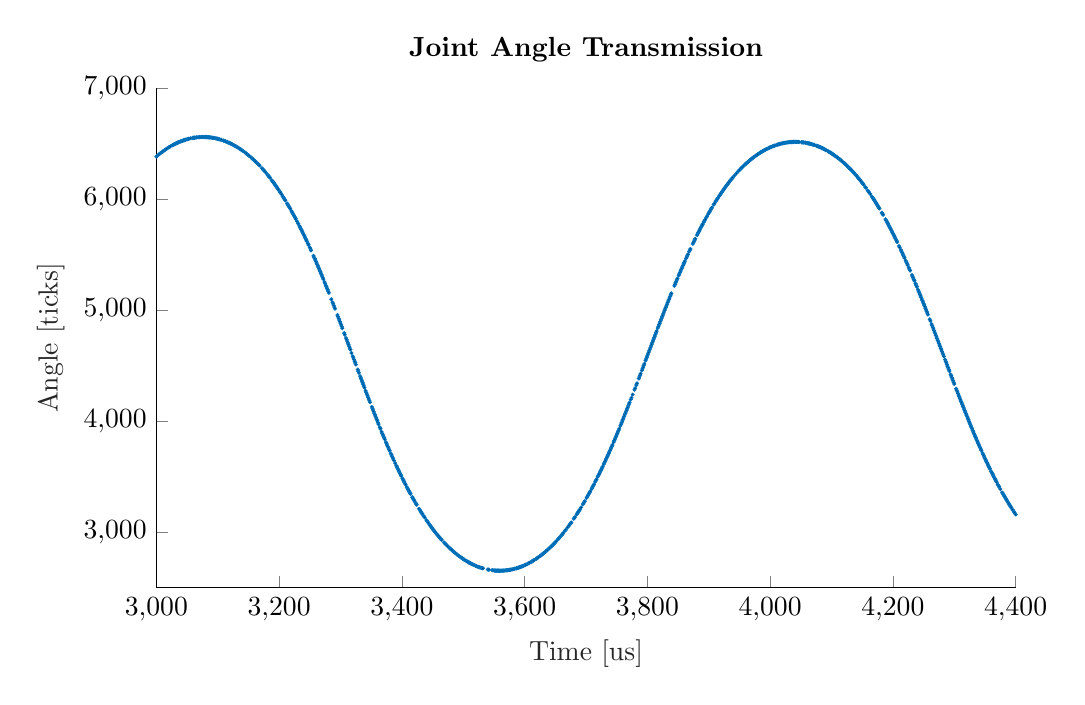
\begin{tikzpicture}

\begin{axis}[%
width=.9\textwidth,
height=2.5in,
at={(0.758in,0.481in)},
scale only axis,
xmin=3000,
xmax=4400,
xlabel style={font=\color{white!15!black}},
xlabel={Time [us]},
ymin=2500,
ymax=7000,
ylabel style={font=\color{white!15!black}},
ylabel={Angle [ticks]},
axis background/.style={fill=white},
title style={font=\bfseries},
title={Joint Angle Transmission},
axis x line*=bottom,
axis y line*=left
]
\addplot[only marks, mark=*, mark options={}, mark size=0.5000pt, draw=mycolor1] table[row sep=crcr]{%
x	y\\
2989	6326\\
2990	6331\\
2991	6337\\
2993	6348\\
2994	6353\\
2995	6358\\
2996	6363\\
2997	6368\\
2998	6373\\
2999	6377\\
3000	6382\\
3001	6387\\
3003	6396\\
3004	6401\\
3006	6410\\
3008	6418\\
3010	6426\\
3011	6430\\
3013	6438\\
3014	6442\\
3016	6450\\
3017	6453\\
3020	6464\\
3021	6467\\
3023	6474\\
3026	6483\\
3027	6486\\
3028	6489\\
3029	6492\\
3030	6495\\
3031	6497\\
3032	6500\\
3033	6503\\
3034	6505\\
3035	6508\\
3036	6510\\
3037	6513\\
3039	6517\\
3040	6519\\
3041	6521\\
3042	6523\\
3043	6525\\
3044	6527\\
3045	6529\\
3046	6531\\
3047	6533\\
3048	6534\\
3050	6538\\
3051	6539\\
3052	6541\\
3053	6542\\
3056	6546\\
3059	6549\\
3060	6550\\
3061	6551\\
3062	6552\\
3063	6553\\
3065	6554\\
3066	6555\\
3068	6556\\
3070	6556\\
3071	6557\\
3073	6557\\
3075	6558\\
3076	6558\\
3078	6558\\
3079	6557\\
3080	6557\\
3081	6557\\
3082	6557\\
3083	6556\\
3084	6556\\
3085	6555\\
3086	6555\\
3087	6554\\
3088	6554\\
3090	6552\\
3091	6551\\
3092	6551\\
3094	6549\\
3096	6546\\
3098	6544\\
3099	6543\\
3100	6541\\
3101	6540\\
3102	6538\\
3103	6537\\
3105	6534\\
3106	6532\\
3109	6526\\
3110	6524\\
3112	6520\\
3113	6518\\
3115	6514\\
3116	6511\\
3118	6507\\
3119	6504\\
3120	6501\\
3121	6499\\
3122	6496\\
3123	6493\\
3124	6490\\
3126	6484\\
3127	6481\\
3129	6475\\
3130	6472\\
3132	6465\\
3134	6459\\
3136	6451\\
3137	6448\\
3138	6444\\
3140	6436\\
3141	6432\\
3144	6420\\
3146	6412\\
3147	6407\\
3149	6398\\
3150	6394\\
3151	6389\\
3154	6375\\
3156	6365\\
3157	6360\\
3158	6355\\
3160	6345\\
3161	6339\\
3162	6334\\
3164	6323\\
3165	6318\\
3166	6312\\
3167	6307\\
3168	6301\\
3172	6277\\
3174	6265\\
3175	6258\\
3176	6252\\
3178	6239\\
3181	6219\\
3182	6212\\
3183	6205\\
3184	6198\\
3185	6191\\
3188	6169\\
3189	6162\\
3190	6154\\
3191	6147\\
3192	6139\\
3193	6131\\
3194	6123\\
3195	6115\\
3196	6107\\
3197	6099\\
3198	6091\\
3199	6083\\
3201	6066\\
3202	6058\\
3204	6041\\
3206	6023\\
3207	6014\\
3208	6006\\
3209	5996\\
3210	5987\\
3213	5960\\
3214	5951\\
3215	5941\\
3216	5931\\
3217	5922\\
3218	5912\\
3220	5892\\
3221	5882\\
3222	5873\\
3223	5863\\
3224	5853\\
3225	5842\\
3226	5832\\
3227	5821\\
3229	5800\\
3231	5779\\
3233	5758\\
3234	5747\\
3235	5735\\
3236	5724\\
3237	5713\\
3238	5702\\
3239	5691\\
3240	5679\\
3241	5668\\
3242	5657\\
3243	5645\\
3244	5633\\
3245	5621\\
3247	5598\\
3248	5586\\
3250	5562\\
3251	5550\\
3252	5537\\
3256	5488\\
3257	5475\\
3258	5463\\
3259	5450\\
3260	5437\\
3261	5424\\
3262	5411\\
3263	5398\\
3264	5385\\
3265	5372\\
3266	5359\\
3267	5346\\
3268	5333\\
3269	5319\\
3270	5306\\
3271	5292\\
3272	5279\\
3274	5252\\
3275	5238\\
3276	5224\\
3277	5210\\
3278	5196\\
3279	5183\\
3280	5169\\
3281	5155\\
3285	5098\\
3287	5070\\
3288	5056\\
3289	5041\\
3290	5027\\
3291	5012\\
3295	4955\\
3296	4940\\
3297	4925\\
3298	4911\\
3299	4896\\
3300	4882\\
3301	4867\\
3302	4852\\
3303	4837\\
3306	4793\\
3307	4778\\
3309	4749\\
3310	4734\\
3311	4719\\
3312	4704\\
3313	4689\\
3314	4674\\
3315	4659\\
3316	4644\\
3318	4614\\
3320	4584\\
3321	4570\\
3322	4555\\
3323	4540\\
3324	4525\\
3325	4510\\
3328	4465\\
3329	4450\\
3330	4435\\
3332	4405\\
3333	4390\\
3334	4376\\
3335	4361\\
3336	4346\\
3337	4332\\
3338	4317\\
3339	4302\\
3341	4273\\
3342	4258\\
3343	4244\\
3344	4229\\
3345	4214\\
3346	4200\\
3347	4185\\
3348	4171\\
3351	4129\\
3352	4114\\
3353	4100\\
3354	4086\\
3355	4072\\
3356	4058\\
3357	4044\\
3358	4030\\
3359	4017\\
3360	4003\\
3361	3987\\
3362	3973\\
3364	3945\\
3365	3932\\
3367	3904\\
3368	3890\\
3369	3877\\
3370	3864\\
3371	3851\\
3372	3838\\
3374	3811\\
3375	3798\\
3376	3785\\
3377	3772\\
3378	3760\\
3379	3747\\
3380	3734\\
3382	3709\\
3383	3697\\
3384	3684\\
3385	3672\\
3386	3660\\
3387	3647\\
3389	3623\\
3391	3599\\
3392	3587\\
3393	3575\\
3394	3564\\
3395	3552\\
3396	3541\\
3397	3529\\
3398	3518\\
3399	3506\\
3401	3484\\
3402	3473\\
3403	3462\\
3404	3451\\
3405	3440\\
3406	3429\\
3408	3408\\
3409	3397\\
3410	3387\\
3411	3376\\
3412	3366\\
3413	3356\\
3414	3346\\
3417	3316\\
3418	3306\\
3419	3296\\
3420	3286\\
3422	3267\\
3423	3258\\
3424	3248\\
3428	3212\\
3429	3203\\
3430	3194\\
3431	3185\\
3432	3176\\
3433	3167\\
3435	3150\\
3436	3142\\
3437	3134\\
3440	3109\\
3441	3101\\
3442	3093\\
3443	3085\\
3445	3069\\
3446	3062\\
3447	3054\\
3448	3047\\
3449	3039\\
3450	3032\\
3451	3024\\
3452	3017\\
3453	3010\\
3454	3003\\
3456	2989\\
3457	2982\\
3458	2976\\
3459	2969\\
3461	2956\\
3462	2950\\
3463	2943\\
3464	2937\\
3465	2931\\
3469	2907\\
3470	2901\\
3471	2895\\
3472	2889\\
3473	2884\\
3475	2873\\
3477	2862\\
3478	2857\\
3479	2852\\
3480	2847\\
3481	2842\\
3483	2832\\
3484	2827\\
3485	2822\\
3486	2817\\
3487	2813\\
3489	2804\\
3490	2799\\
3492	2791\\
3493	2787\\
3494	2782\\
3496	2775\\
3497	2771\\
3498	2767\\
3499	2763\\
3500	2759\\
3501	2756\\
3502	2752\\
3505	2742\\
3506	2739\\
3508	2732\\
3509	2729\\
3510	2726\\
3511	2723\\
3512	2720\\
3513	2717\\
3515	2712\\
3516	2709\\
3518	2704\\
3520	2699\\
3521	2697\\
3522	2695\\
3524	2690\\
3525	2688\\
3526	2686\\
3527	2684\\
3529	2681\\
3530	2679\\
3531	2677\\
3532	2676\\
3540	2665\\
3541	2664\\
3542	2663\\
3547	2659\\
3548	2658\\
3550	2657\\
3551	2656\\
3552	2656\\
3553	2655\\
3554	2655\\
3555	2655\\
3556	2655\\
3557	2655\\
3558	2654\\
3559	2654\\
3560	2654\\
3561	2654\\
3562	2655\\
3564	2655\\
3565	2655\\
3566	2656\\
3567	2656\\
3569	2657\\
3570	2658\\
3571	2658\\
3572	2659\\
3574	2661\\
3575	2662\\
3576	2663\\
3577	2664\\
3578	2665\\
3580	2667\\
3581	2668\\
3583	2671\\
3584	2672\\
3586	2675\\
3587	2677\\
3588	2679\\
3589	2680\\
3590	2682\\
3591	2684\\
3592	2686\\
3593	2688\\
3594	2690\\
3595	2692\\
3596	2694\\
3597	2697\\
3598	2699\\
3600	2704\\
3601	2706\\
3602	2709\\
3604	2714\\
3605	2717\\
3607	2723\\
3608	2726\\
3611	2735\\
3612	2738\\
3613	2742\\
3614	2745\\
3615	2748\\
3618	2759\\
3619	2762\\
3620	2766\\
3621	2770\\
3622	2774\\
3625	2786\\
3626	2790\\
3627	2794\\
3628	2799\\
3629	2803\\
3630	2807\\
3631	2812\\
3632	2816\\
3634	2826\\
3635	2831\\
3636	2836\\
3637	2840\\
3639	2851\\
3640	2856\\
3641	2861\\
3643	2871\\
3644	2877\\
3645	2882\\
3646	2888\\
3647	2893\\
3648	2899\\
3649	2905\\
3650	2911\\
3651	2917\\
3654	2935\\
3655	2941\\
3656	2948\\
3658	2960\\
3660	2973\\
3661	2980\\
3662	2987\\
3663	2994\\
3666	3015\\
3667	3022\\
3670	3044\\
3672	3059\\
3674	3074\\
3675	3082\\
3676	3089\\
3680	3122\\
3681	3130\\
3682	3138\\
3685	3163\\
3686	3172\\
3687	3181\\
3688	3189\\
3689	3198\\
3690	3207\\
3692	3225\\
3695	3253\\
3696	3262\\
3697	3272\\
3698	3281\\
3701	3310\\
3702	3320\\
3703	3330\\
3704	3340\\
3705	3350\\
3706	3360\\
3707	3370\\
3709	3391\\
3710	3401\\
3711	3412\\
3712	3422\\
3713	3433\\
3715	3455\\
3716	3465\\
3717	3476\\
3719	3499\\
3720	3510\\
3721	3521\\
3722	3532\\
3723	3544\\
3724	3555\\
3725	3567\\
3726	3578\\
3727	3590\\
3729	3614\\
3730	3626\\
3731	3638\\
3732	3650\\
3733	3662\\
3734	3674\\
3735	3686\\
3736	3698\\
3737	3711\\
3738	3723\\
3739	3736\\
3740	3749\\
3741	3761\\
3742	3774\\
3743	3786\\
3745	3812\\
3746	3825\\
3747	3838\\
3748	3851\\
3749	3864\\
3750	3877\\
3751	3891\\
3752	3904\\
3753	3917\\
3754	3931\\
3756	3958\\
3757	3972\\
3758	3986\\
3759	4002\\
3760	4015\\
3761	4029\\
3762	4043\\
3763	4057\\
3764	4070\\
3765	4084\\
3766	4098\\
3767	4112\\
3768	4126\\
3769	4140\\
3770	4154\\
3771	4168\\
3773	4196\\
3774	4211\\
3776	4239\\
3779	4283\\
3780	4297\\
3782	4326\\
3783	4341\\
3786	4384\\
3787	4399\\
3788	4413\\
3789	4428\\
3791	4458\\
3792	4472\\
3793	4487\\
3794	4502\\
3795	4516\\
3797	4546\\
3798	4561\\
3799	4575\\
3800	4590\\
3801	4605\\
3802	4619\\
3803	4634\\
3804	4649\\
3805	4663\\
3806	4678\\
3807	4693\\
3808	4707\\
3809	4722\\
3810	4737\\
3811	4751\\
3812	4766\\
3813	4781\\
3814	4795\\
3815	4810\\
3817	4839\\
3818	4854\\
3819	4868\\
3820	4882\\
3821	4897\\
3822	4911\\
3823	4925\\
3824	4940\\
3825	4954\\
3826	4968\\
3827	4982\\
3828	4997\\
3829	5011\\
3830	5025\\
3831	5039\\
3832	5053\\
3833	5067\\
3834	5081\\
3835	5095\\
3836	5109\\
3837	5123\\
3838	5137\\
3839	5151\\
3844	5219\\
3845	5232\\
3846	5246\\
3847	5259\\
3848	5272\\
3849	5285\\
3851	5312\\
3852	5325\\
3853	5338\\
3854	5351\\
3855	5364\\
3856	5377\\
3857	5389\\
3858	5402\\
3859	5415\\
3860	5427\\
3861	5440\\
3863	5465\\
3864	5477\\
3865	5489\\
3866	5501\\
3868	5526\\
3869	5538\\
3870	5550\\
3874	5596\\
3875	5608\\
3876	5620\\
3877	5631\\
3878	5642\\
3881	5676\\
3882	5687\\
3883	5698\\
3884	5709\\
3885	5720\\
3886	5731\\
3887	5741\\
3888	5752\\
3889	5763\\
3890	5773\\
3892	5793\\
3893	5804\\
3894	5814\\
3896	5834\\
3897	5844\\
3899	5864\\
3900	5874\\
3901	5883\\
3902	5892\\
3903	5902\\
3904	5912\\
3905	5921\\
3908	5949\\
3909	5958\\
3911	5975\\
3912	5984\\
3913	5993\\
3914	6001\\
3915	6010\\
3917	6027\\
3918	6035\\
3919	6043\\
3920	6052\\
3921	6060\\
3922	6068\\
3923	6076\\
3924	6083\\
3925	6091\\
3926	6099\\
3927	6107\\
3928	6114\\
3929	6122\\
3930	6129\\
3931	6136\\
3932	6144\\
3933	6151\\
3935	6165\\
3936	6172\\
3937	6179\\
3938	6185\\
3939	6192\\
3942	6212\\
3945	6231\\
3948	6249\\
3949	6255\\
3950	6261\\
3952	6272\\
3953	6278\\
3954	6283\\
3956	6294\\
3957	6299\\
3959	6310\\
3960	6315\\
3961	6320\\
3962	6325\\
3963	6330\\
3964	6334\\
3966	6344\\
3967	6349\\
3968	6353\\
3969	6358\\
3970	6362\\
3971	6367\\
3972	6371\\
3973	6375\\
3974	6379\\
3976	6387\\
3977	6391\\
3979	6399\\
3980	6403\\
3982	6410\\
3983	6414\\
3984	6417\\
3985	6421\\
3986	6424\\
3987	6427\\
3988	6431\\
3989	6434\\
3990	6437\\
3991	6440\\
3992	6443\\
3993	6446\\
3995	6452\\
3997	6457\\
3998	6460\\
3999	6462\\
4000	6465\\
4001	6467\\
4002	6469\\
4004	6474\\
4005	6476\\
4007	6480\\
4008	6482\\
4011	6487\\
4012	6489\\
4013	6491\\
4014	6492\\
4015	6494\\
4016	6496\\
4017	6497\\
4019	6500\\
4020	6501\\
4022	6503\\
4023	6505\\
4025	6506\\
4027	6508\\
4028	6509\\
4030	6510\\
4032	6512\\
4033	6512\\
4034	6512\\
4035	6513\\
4036	6513\\
4037	6513\\
4038	6514\\
4039	6514\\
4041	6514\\
4042	6514\\
4043	6514\\
4044	6514\\
4046	6513\\
4047	6513\\
4051	6511\\
4052	6510\\
4053	6510\\
4054	6509\\
4055	6508\\
4057	6507\\
4058	6506\\
4060	6504\\
4061	6502\\
4062	6501\\
4063	6500\\
4064	6499\\
4065	6497\\
4066	6496\\
4067	6494\\
4069	6491\\
4070	6489\\
4071	6488\\
4072	6486\\
4075	6480\\
4076	6478\\
4077	6476\\
4078	6474\\
4079	6472\\
4080	6470\\
4081	6467\\
4082	6465\\
4083	6462\\
4084	6460\\
4085	6457\\
4086	6455\\
4087	6452\\
4088	6449\\
4089	6446\\
4091	6440\\
4094	6431\\
4095	6428\\
4096	6424\\
4097	6421\\
4098	6418\\
4099	6414\\
4100	6411\\
4101	6407\\
4102	6403\\
4103	6399\\
4104	6395\\
4105	6391\\
4106	6387\\
4108	6380\\
4109	6375\\
4110	6371\\
4112	6363\\
4113	6359\\
4114	6354\\
4115	6349\\
4116	6345\\
4118	6335\\
4120	6326\\
4121	6321\\
4122	6316\\
4123	6311\\
4124	6306\\
4125	6300\\
4126	6295\\
4127	6289\\
4128	6284\\
4129	6279\\
4130	6273\\
4131	6268\\
4132	6262\\
4134	6250\\
4135	6244\\
4136	6238\\
4137	6232\\
4139	6219\\
4140	6213\\
4141	6207\\
4143	6193\\
4144	6187\\
4145	6180\\
4146	6173\\
4147	6166\\
4149	6152\\
4150	6145\\
4151	6138\\
4152	6131\\
4155	6108\\
4156	6101\\
4159	6077\\
4160	6069\\
4161	6061\\
4163	6045\\
4166	6020\\
4167	6012\\
4168	6003\\
4169	5995\\
4170	5986\\
4171	5977\\
4172	5968\\
4173	5960\\
4174	5951\\
4175	5941\\
4176	5932\\
4177	5923\\
4178	5914\\
4182	5876\\
4183	5866\\
4184	5857\\
4188	5817\\
4189	5807\\
4190	5796\\
4191	5786\\
4192	5776\\
4193	5765\\
4194	5755\\
4195	5744\\
4196	5733\\
4197	5723\\
4198	5712\\
4199	5701\\
4200	5690\\
4201	5679\\
4202	5668\\
4203	5657\\
4204	5646\\
4205	5634\\
4206	5623\\
4207	5612\\
4210	5577\\
4211	5565\\
4213	5541\\
4214	5529\\
4215	5517\\
4216	5505\\
4217	5493\\
4218	5481\\
4219	5469\\
4221	5444\\
4222	5431\\
4223	5419\\
4224	5406\\
4226	5381\\
4227	5368\\
4228	5355\\
4231	5316\\
4232	5303\\
4233	5290\\
4234	5277\\
4235	5264\\
4237	5237\\
4238	5223\\
4239	5210\\
4241	5183\\
4242	5169\\
4243	5156\\
4244	5142\\
4245	5128\\
4246	5114\\
4247	5100\\
4248	5086\\
4249	5073\\
4250	5059\\
4251	5045\\
4252	5031\\
4253	5016\\
4254	5002\\
4255	4988\\
4256	4974\\
4257	4960\\
4260	4917\\
4261	4903\\
4263	4874\\
4264	4860\\
4265	4845\\
4266	4831\\
4267	4816\\
4268	4802\\
4269	4787\\
4270	4773\\
4271	4758\\
4272	4744\\
4273	4729\\
4274	4714\\
4275	4700\\
4276	4685\\
4277	4671\\
4278	4656\\
4279	4642\\
4280	4627\\
4281	4612\\
4282	4598\\
4283	4583\\
4285	4554\\
4286	4539\\
4287	4525\\
4288	4510\\
4289	4495\\
4290	4481\\
4291	4466\\
4292	4452\\
4294	4422\\
4295	4408\\
4296	4393\\
4297	4379\\
4298	4364\\
4299	4350\\
4300	4335\\
4303	4292\\
4304	4278\\
4305	4264\\
4306	4249\\
4307	4235\\
4308	4221\\
4309	4207\\
4310	4192\\
4311	4178\\
4312	4165\\
4313	4151\\
4314	4137\\
4315	4123\\
4316	4109\\
4317	4095\\
4318	4081\\
4319	4068\\
4320	4054\\
4321	4040\\
4322	4027\\
4323	4013\\
4324	3998\\
4325	3984\\
4326	3971\\
4327	3957\\
4328	3944\\
4329	3931\\
4330	3917\\
4331	3903\\
4332	3890\\
4333	3877\\
4334	3864\\
4335	3852\\
4336	3839\\
4337	3826\\
4338	3813\\
4339	3800\\
4340	3787\\
4341	3775\\
4342	3763\\
4343	3750\\
4344	3738\\
4346	3713\\
4347	3701\\
4348	3689\\
4349	3677\\
4350	3665\\
4351	3653\\
4352	3641\\
4353	3630\\
4354	3618\\
4355	3606\\
4356	3594\\
4357	3583\\
4358	3572\\
4360	3549\\
4361	3538\\
4362	3527\\
4363	3516\\
4364	3505\\
4365	3494\\
4366	3483\\
4367	3473\\
4368	3462\\
4369	3451\\
4371	3430\\
4372	3420\\
4373	3410\\
4375	3389\\
4378	3359\\
4379	3350\\
4380	3340\\
4381	3330\\
4382	3321\\
4383	3311\\
4384	3302\\
4385	3292\\
4386	3283\\
4387	3274\\
4388	3265\\
4389	3256\\
4390	3247\\
4391	3238\\
4392	3229\\
4393	3220\\
4395	3203\\
4397	3186\\
4398	3178\\
4400	3161\\
4401	3153\\
4402	3145\\
4403	3137\\
4404	3129\\
4405	3121\\
4408	3098\\
4409	3091\\
4410	3083\\
4411	3076\\
4412	3069\\
4413	3061\\
4414	3054\\
4415	3047\\
4416	3040\\
4418	3027\\
4419	3020\\
4420	3013\\
4421	3007\\
4423	2994\\
4424	2987\\
4425	2981\\
4427	2969\\
4428	2963\\
4429	2957\\
4431	2945\\
4432	2939\\
4433	2933\\
4435	2922\\
4436	2917\\
4439	2901\\
4440	2895\\
4441	2890\\
4443	2880\\
4444	2875\\
4445	2871\\
4446	2866\\
4447	2861\\
4448	2857\\
4450	2848\\
4451	2843\\
4454	2830\\
4455	2826\\
4456	2822\\
4458	2814\\
4459	2810\\
4461	2803\\
4462	2799\\
4463	2796\\
4465	2789\\
4466	2785\\
4468	2779\\
4469	2776\\
4472	2766\\
4474	2761\\
4475	2758\\
4476	2755\\
4477	2753\\
4478	2750\\
4479	2748\\
4481	2743\\
4483	2738\\
4484	2736\\
4486	2732\\
4487	2730\\
4488	2728\\
4490	2724\\
4495	2716\\
4496	2714\\
4497	2713\\
4499	2710\\
4501	2708\\
4502	2707\\
4503	2706\\
4504	2705\\
4505	2704\\
4507	2702\\
4508	2701\\
4510	2700\\
4511	2700\\
4512	2699\\
4513	2699\\
4514	2698\\
4516	2698\\
4518	2697\\
4519	2697\\
4520	2697\\
4521	2697\\
4522	2697\\
4523	2697\\
4524	2697\\
4525	2698\\
4527	2698\\
4528	2699\\
4529	2699\\
4530	2700\\
4533	2702\\
4534	2703\\
4535	2703\\
4537	2705\\
4538	2706\\
4539	2707\\
4541	2710\\
4542	2711\\
4544	2714\\
4545	2715\\
4547	2718\\
4548	2720\\
4550	2723\\
4551	2725\\
4553	2729\\
4557	2737\\
4558	2740\\
4559	2742\\
4560	2744\\
4561	2747\\
4562	2749\\
4563	2752\\
4564	2754\\
4565	2757\\
4566	2760\\
4567	2763\\
4569	2768\\
4570	2771\\
4571	2775\\
4572	2778\\
4573	2781\\
4576	2791\\
4577	2794\\
4578	2798\\
4579	2802\\
4580	2805\\
4581	2809\\
4583	2817\\
4584	2821\\
4585	2825\\
4586	2829\\
4587	2833\\
4588	2837\\
4589	2842\\
4590	2846\\
4591	2850\\
4592	2855\\
4593	2859\\
4594	2864\\
4595	2869\\
4596	2874\\
4597	2878\\
4598	2883\\
4601	2898\\
4602	2904\\
4604	2914\\
4605	2920\\
4606	2925\\
4607	2931\\
4608	2937\\
4610	2948\\
4611	2954\\
4612	2960\\
4613	2966\\
4614	2972\\
4620	3010\\
4621	3016\\
4622	3023\\
4624	3037\\
4625	3044\\
4626	3051\\
4628	3065\\
4629	3072\\
4630	3079\\
4631	3087\\
4633	3102\\
4634	3109\\
4636	3125\\
4638	3140\\
4639	3148\\
4640	3156\\
4643	3181\\
4644	3189\\
4645	3198\\
4646	3206\\
4648	3223\\
4649	3232\\
4650	3241\\
4651	3250\\
4652	3259\\
4653	3268\\
4654	3277\\
4655	3286\\
4657	3304\\
4658	3314\\
4659	3323\\
4661	3342\\
4662	3352\\
4663	3362\\
4664	3372\\
4665	3382\\
4666	3392\\
4667	3402\\
4669	3422\\
4670	3433\\
4671	3443\\
4672	3453\\
4674	3474\\
4675	3485\\
4676	3496\\
4677	3507\\
4682	3562\\
4684	3584\\
4685	3596\\
4687	3619\\
4688	3631\\
4689	3642\\
4690	3654\\
4696	3726\\
4697	3738\\
4699	3762\\
4700	3775\\
4701	3787\\
4702	3799\\
4703	3812\\
4704	3825\\
4705	3838\\
4707	3863\\
4708	3876\\
4709	3889\\
4711	3915\\
4712	3928\\
4713	3942\\
4714	3955\\
4715	3968\\
4716	3982\\
4717	3995\\
4718	4010\\
4719	4024\\
4720	4037\\
4722	4064\\
4724	4091\\
4725	4105\\
4726	4118\\
4728	4146\\
4729	4160\\
4731	4187\\
4733	4215\\
4734	4229\\
4735	4243\\
4736	4258\\
4738	4286\\
4740	4314\\
4741	4328\\
4742	4343\\
4747	4414\\
4748	4428\\
4749	4443\\
4750	4457\\
4752	4486\\
4753	4500\\
4754	4515\\
4755	4529\\
4756	4544\\
4757	4558\\
4758	4573\\
4760	4601\\
4761	4616\\
4762	4630\\
4763	4645\\
4764	4659\\
4765	4673\\
4767	4702\\
4768	4716\\
4769	4731\\
4770	4745\\
4771	4760\\
4772	4774\\
4773	4788\\
4774	4802\\
4775	4817\\
4776	4831\\
4780	4887\\
4781	4902\\
4782	4916\\
4784	4944\\
4785	4958\\
4787	4985\\
4789	5013\\
4790	5027\\
4793	5069\\
4794	5082\\
4796	5110\\
4797	5123\\
4798	5137\\
4799	5150\\
4800	5164\\
4801	5177\\
4802	5190\\
4803	5203\\
4804	5217\\
4805	5230\\
4806	5243\\
4808	5269\\
4809	5282\\
4810	5295\\
4811	5308\\
4813	5333\\
4814	5346\\
4815	5359\\
4818	5396\\
4819	5408\\
4821	5433\\
4823	5458\\
4824	5469\\
4825	5481\\
4826	5493\\
4827	5505\\
4828	5517\\
4829	5529\\
4830	5540\\
4831	5552\\
4832	5563\\
4833	5575\\
4834	5586\\
4835	5597\\
4838	5631\\
4839	5642\\
4840	5653\\
4841	5664\\
4842	5675\\
4843	5685\\
4844	5696\\
4847	5727\\
4848	5738\\
4849	5748\\
4850	5758\\
4851	5768\\
4853	5788\\
4855	5808\\
4857	5828\\
4858	5837\\
4859	5847\\
4860	5857\\
4861	5866\\
4863	5884\\
4864	5893\\
4865	5903\\
4866	5912\\
4868	5930\\
4869	5938\\
4870	5947\\
4872	5964\\
4874	5981\\
4875	5989\\
4876	5998\\
4877	6006\\
4878	6014\\
4879	6022\\
4880	6030\\
4881	6038\\
4882	6046\\
4883	6054\\
4884	6061\\
4885	6069\\
4886	6076\\
4888	6091\\
4889	6098\\
4890	6105\\
4891	6113\\
4892	6120\\
4894	6134\\
4896	6147\\
4897	6154\\
4898	6160\\
4899	6167\\
4900	6173\\
4903	6192\\
4904	6198\\
4905	6204\\
4907	6216\\
4908	6222\\
4911	6239\\
4912	6245\\
4913	6250\\
4914	6256\\
4915	6261\\
4919	6281\\
4921	6291\\
4922	6296\\
4923	6300\\
4924	6305\\
4926	6314\\
4927	6319\\
4929	6327\\
4932	6340\\
4933	6344\\
4934	6348\\
4935	6352\\
4936	6356\\
4937	6360\\
4938	6363\\
4939	6367\\
4940	6370\\
4941	6374\\
4942	6377\\
4943	6381\\
4944	6384\\
4945	6387\\
4946	6390\\
4948	6397\\
4949	6400\\
4950	6403\\
4951	6406\\
4952	6408\\
4953	6411\\
4954	6414\\
4955	6416\\
4960	6429\\
4961	6431\\
4962	6433\\
4964	6437\\
4965	6439\\
4967	6443\\
4968	6445\\
4970	6449\\
4971	6450\\
4972	6452\\
4974	6455\\
4975	6456\\
};
\end{axis}
\end{tikzpicture}%
	\caption[One period joint angle data]{One period joint angle data. A full rotation is equal to 7200 ticks.}
	\label{fig:joint_angle_measured_zoom}
\end{figure}
From figures \ref{fig:joint_angle_measured_full} and \ref{fig:joint_angle_measured_zoom} it can be verified that the joint angle are measured correctly as all data is as expected.
\\~\\
The full test was only realised on one of the joint boards, as only one board was finished due to time constraints.


\subsection{Verification of: Requirement \ref{enum:software_developed_real_time}} % (fold)
\label{sub:verification_of_requirement_enum:software_developed_real_time}
This requirement specifies that any software developed for the pendulum system should be real-time.

\paragraph{Conclusion}~\\
In section \ref{ssub:verification_of_requirement_of_requirement_enum:real_time_behavior} it is described that due to time constraints real-time behaviour of the controller board software was not realised.
\\~\\
\thomas{rewrite to mention no completed system instead}
In section \ref{ssub:requirement_enum_joint_real_time} it is tested and verified that the joint board software is real-time.


\subsection{Verification of: Requirement \ref{enum:system_accessible_to_users}} % (fold)
\label{sub:verification_of_requirement_enum:system_accessible_to_users}
This requirement states that the system should be easily accessible to users.

\paragraph{Conclusion}~\\
Throughout the design of the system, accessibility has been a focus.
Section \ref{ssub:requirement_enum:pcb_debugging} describes how the PCB has been desgined with debugging in mind.
Verification procedures have been developed for the joint and controller boards and is included in the report as appendix \ref{sec:joint_board_verification_procedure} and \ref{sec:controller_board_verification_procedure}.
\\~\\
The usability of the controller board should be verified by using students as test subjects once the system is finished. 

\subsection{Verification of: Requirement \ref{enum:system_should_not_break_during_operation}} % (fold)
\label{sub:verification_of_requirement_enum:system_should_not_break_during_operation}
This requirement specifies that the system should not break during operation by users.

\paragraph{Conclusion}~\\
The design of the controller board electronics is done with the requirement that the components should be able to handle the stall current of the motor.
\\
Section \ref{ssub:requirement_enum:any_trigger_em} verifies that the implemented endstops can cut off power to the H-bridge effectively stopping the motor.

\subsection{Verification of: Requirement \ref{enum:safety_should_not_rely_on_programming}} % (fold)
\label{sub:verification_of_requirement_enum:safety_should_not_rely_on_programming}
According to this requirement the system safety should not rely on the programming of the system.

\paragraph{Conclusion}~\\
Signals from endstops and emergency button cuts off power to the H-bridge through digital electronics.
The functionality is verified in section \ref{ssub:requirement_enum:any_trigger_em}.

\subsection{Verification of: Requirement \ref{enum:software_top_down_bottom_up}} % (fold)
\label{sub:verification_of_requirement_enum:software_top_down_bottom_up}
This requirement states that software design should be done top-down, whereas subcomponents are written bottom-up.

\paragraph{Conclusion}~\\
This design procedure was followed while designing software for the joint and controller boards.